% 文章クラス:1段組のA4報告書(和文)
\documentclass[a4j,11pt]{jreport}
\usepackage{amssymb}
\usepackage{multirow} 
\usepackage{midpage}

% 文字のフォント指定
\usepackage{mathptmx}
\usepackage{newtxtext,newtxmath}
% \usepackage{titlesec}
% \titleformat*{\section}{\fontsize{12pt}{10pt}\selectfont\bf}
% \titleformat*{\subsection}{\fontsize{10pt}{10pt}\selectfont\bf}

\usepackage{titlesec}
\titleformat*{\section}{\fontsize{14pt}{0pt}\selectfont\bf}
\titleformat*{\subsection}{\fontsize{12pt}{0pt}\selectfont\bf}

\usepackage{setspace}
\usepackage{otf}%はしご高用
\setstretch{1.2}


%ヘッダーの設定
% \usepackage{fancyhdr}
% \usepackage{otf}
%  \pagestyle{fancy}
%     \lhead{\fontsize{10pt}{0pt}\selectfont{\ajRoman{2}}}
%      \chead{}
%     \rhead{}
%数式の設定%
\usepackage{amsmath}
%表のページ跨がせるよう%
\usepackage{longtable}
\usepackage{array}

\usepackage{comment}

% 余白の設定(上下左右:2cm)
\usepackage[margin=30truemm]{geometry}

% 図と表の設定
\usepackage[dvipdfmx]{graphicx}
\renewcommand{\figurename}{Fig. }
\renewcommand{\tablename}{Table}
\setlength\intextsep{10pt} % 図の余白
\setlength\textfloatsep{10pt} % 図の余白
\usepackage{here}

%tableやfigure内で図や表を出すためのコマンド
\makeatletter
\newcommand{\figcaption}[1]{\def\@captype{figure}\caption{#1}}
\newcommand{\tblcaption}[1]{\def\@captype{table}\caption{#1}}
\makeatother

% 追加パッケージ
\usepackage{comment}
\usepackage{subcaption}
\usepackage{url}
\usepackage{multicol}
\usepackage{CJKutf8}
\usepackage[dvipdfmx]{hyperref}
\usepackage{pxjahyper}
\usepackage{otf}
\usepackage{cleveref}
\crefname{figure}{Fig.}{Figs.}
\crefname{table}{Tab.}{Tabs.}
\usepackage{bm}
\usepackage{booktabs}
\usepackage{multirow}
\usepackage{siunitx}
\usepackage{minted}

% ドキュメント開始
\begin{document}
% ~~~表紙~~~
\begin{titlepage}
    \begin{center}
        \fontsize{16.060pt}{24.090pt}\selectfont{修士論文}\\
        \vspace{10.5pt}
        \fontsize{16.060pt}{24.090pt}\selectfont{意味的な画像概念のDNN学習過程における汎化性能について}\\
        \vspace{10.5pt}
        \fontsize{12.045pt}{18.067pt}\selectfont{On generalization performance under DNN learning process of semantic image concepts}\\
        \vspace{10.5pt}
        \fontsize{12.045pt}{18.067pt}\selectfont{\quad}\\
        \vspace{10.5pt}
        \fontsize{12.045pt}{18.067pt}\selectfont{\quad}\\
        \vspace{10.5pt}
        \fontsize{12.045pt}{18.067pt}\selectfont{\quad}\\
        \vspace{10.5pt}
        \fontsize{12.045pt}{18.067pt}\selectfont{\quad}\\
        \vspace{10.5pt}
        \fontsize{12.045pt}{18.067pt}\selectfont{\quad}\\
        \vspace{10.5pt}
        \fontsize{12.045pt}{18.067pt}\selectfont{\quad}\\
        \vspace{10.5pt}
        \fontsize{12.045pt}{18.067pt}\selectfont{\quad}\\
        \vspace{10.5pt}
        \fontsize{12.045pt}{18.067pt}\selectfont{\quad}\\
        \vspace{10.5pt}
        \fontsize{12.045pt}{18.067pt}\selectfont{\quad}\\
        \vspace{10.5pt}
        \fontsize{16.060pt}{24.090pt}\selectfont{\quad}\\
        \vspace{10.5pt}
        \fontsize{16.060pt}{24.090pt}\selectfont{東京電機大学大学院 システムデザイン工学研究科}\\
        \vspace{10.5pt}
        \fontsize{16.060pt}{24.090pt}\selectfont{情報システム工学専攻 修士課程}\\
        \vspace{10.5pt}
        \fontsize{16.060pt}{24.090pt}\selectfont{23AMJ03 岩瀬 俊}\\
        \vspace{10.5pt}
        \fontsize{16.060pt}{24.090pt}\selectfont{研究指導教員 \quad 教授 前田 英作}\\
        \vspace{10.5pt}
    \end{center}
\end{titlepage}

% 文章開始


\chapter*{要旨}
深層ニューラルネットワーク(DNN)を用いたエンドツーエンド学習は,コンピュータビジョン(CV)および自然言語処理(NLP)の諸タスクにおいて高い性能を実証している.しかしながら,分散表現に依存するDNNの解釈可能性は依然として限定的であり,ブラックボックスとして扱われることが多い.この透明性の欠如により,DNNが何を,いつ,どのように学習するのかという深層学習のメカニズムに対する深い理解が妨げられている.
複雑な画像認識タスクは一般的に,複数の意味的な画像概念を並行して学習することを伴い,異なる特徴が様々な時間スケールで学習される.従来研究では形状やテクスチャ特徴の学習が分析されてきたが,これらの概念は通常,与えられたデータセットに基づいて帰納的に定義されており,体系的な分析には制限があった.信頼性の高い分析を行うためには,適切かつ制御可能な難易度レベルと,それらを支持するための十分なデータを有する学習タスクの確立が不可欠である.
これらの課題に対し,本研究では「数字」と「色」という2つの解釈可能な概念に着目し,サンプル間に固有のノイズを含むEMNIST Digitsデータセットに色情報を付加することで,100クラスの分類タスクを構築した.その上で,標準的な条件下および追加的なラベルノイズ存在下におけるDNN学習プロセスの分析を実施した.
本研究の結果より,各概念の獲得難度に応じて学習のタイミングが異なること,また異なる概念の学習間に相互作用が存在することが明らかとなった.これらの知見は,深層学習における画像概念の学習プロセスに関する示唆を与えるものであり,画像ベースのタスクを超えた応用可能性を有するとともに,深層学習のダイナミクスの包括的な理解に寄与するものである.
\newpage

\chapter*{Abstract}

End-to-end learning using deep neural networks (DNNs) has demonstrated high performance across various computer vision (CV) and natural language processing (NLP) tasks. However, the interpretability of DNNs, which rely on distributed representations, remains limited, often rendering them as black boxes. This lack of transparency prevents a deeper understanding of the mechanics of deep learning, specifically regarding what, when, and how DNNs learn.
In contrast, complex image recognition tasks generally involve learning multiple semantic image concepts in parallel, with different features learned at varying time scales. While previous studies have analyzed the learning of shape and texture features, these concepts are typically defined inductively based on the given dataset, limiting systematic analysis.
For reliable analysis, it's crucial to establish learning tasks with appropriate, controllable difficulty levels and sufficient data to support them. To address these needs, we focused on two interpretable concepts—"numbers" and "colors"—and developed a classification task with 100 classes by adding color information to the EMNIST Digits dataset, which includes inherent noise across samples. We then analyzed the DNN learning process under standard conditions and with additional label noise.
Our results reveal that the timing of learning differs depending on the difficulty of acquiring each concept and that there is an interaction between learning different concepts. These findings offer insights into the learning process of image concepts in deep learning, with potential applications beyond image-based tasks, contributing to a broader understanding of deep learning dynamics.

\newpage

\tableofcontents
\newpage
\listoffigures
\newpage
\listoftables
\newpage

\chapter{序論}
深層ニューラルネットワーク(DNN)は,画像認識や自然言語処理など,幅広い分野において著しい性能向上を遂げてきた.特に,ImageNetチャレンジにおける成功を契機に,DNNは視覚的タスクにおいて人間の能力を凌駕する成果を示している\cite{ILSVRC15}.しかし,その性能の背後にある内部表現の形成メカニズムは未だ十分に解明されておらず,その「ブラックボックス」的な性質は重要な研究課題として残されている.モデルの信頼性や透明性を高めるためには,学習プロセスにおける視覚的特徴の獲得メカニズムを明らかにする必要がある.

本研究は,DNNの視覚的特徴の学習プロセスにおいて,特徴獲得の順序や相互作用のメカニズムを明らかにすることを目的とする.特に,学習過程における内部表現の動的変化を系統的に分析するため,新しい実験的枠組みを構築する.視覚的特徴として「数字」と「色」に注目し,データセットを制御することで,学習過程を観察可能な環境を整備する.

本研究では,EMNIST Digitsデータセットに色情報を付加し,視覚的特徴の学習ダイナミクスを解析するための制御可能なデータセットを構築する.これにより,視覚的特徴の学習順序,獲得速度,および特徴間の相互作用を詳細に分析する.学習過程の評価には,モデルの精度を色や数字のみのエラー率に分解し,概念ごとの精度を観察する.
% ,特徴マップの可視化\cite{DBLP:conf/cvpr/ZeilerF14},内部表現のクラスタリング結果など,多角的な評価指標を用いる.

本研究の貢献は以下の3点に要約される.第一に,DNNの学習プロセスを解析するための制御可能な実験環境を構築した.第二に,異なる視覚的特徴の学習順序および相互作用を定量的に評価し,特徴獲得メカニズムを明らかにした.第三に,学習環境におけるノイズの影響を詳細に調査し,モデルのロバスト性と学習効率に関する重要な知見を得た\cite{DBLP:conf/icml/BahdanauCB14}.

これらの成果は,深層学習における内部表現の理解を深めるとともに,効率的かつ解釈可能な学習アルゴリズムの設計に向けた新たな指針を提供するものである.
\newpage
% \begin{figure}[t]
% \centering
% 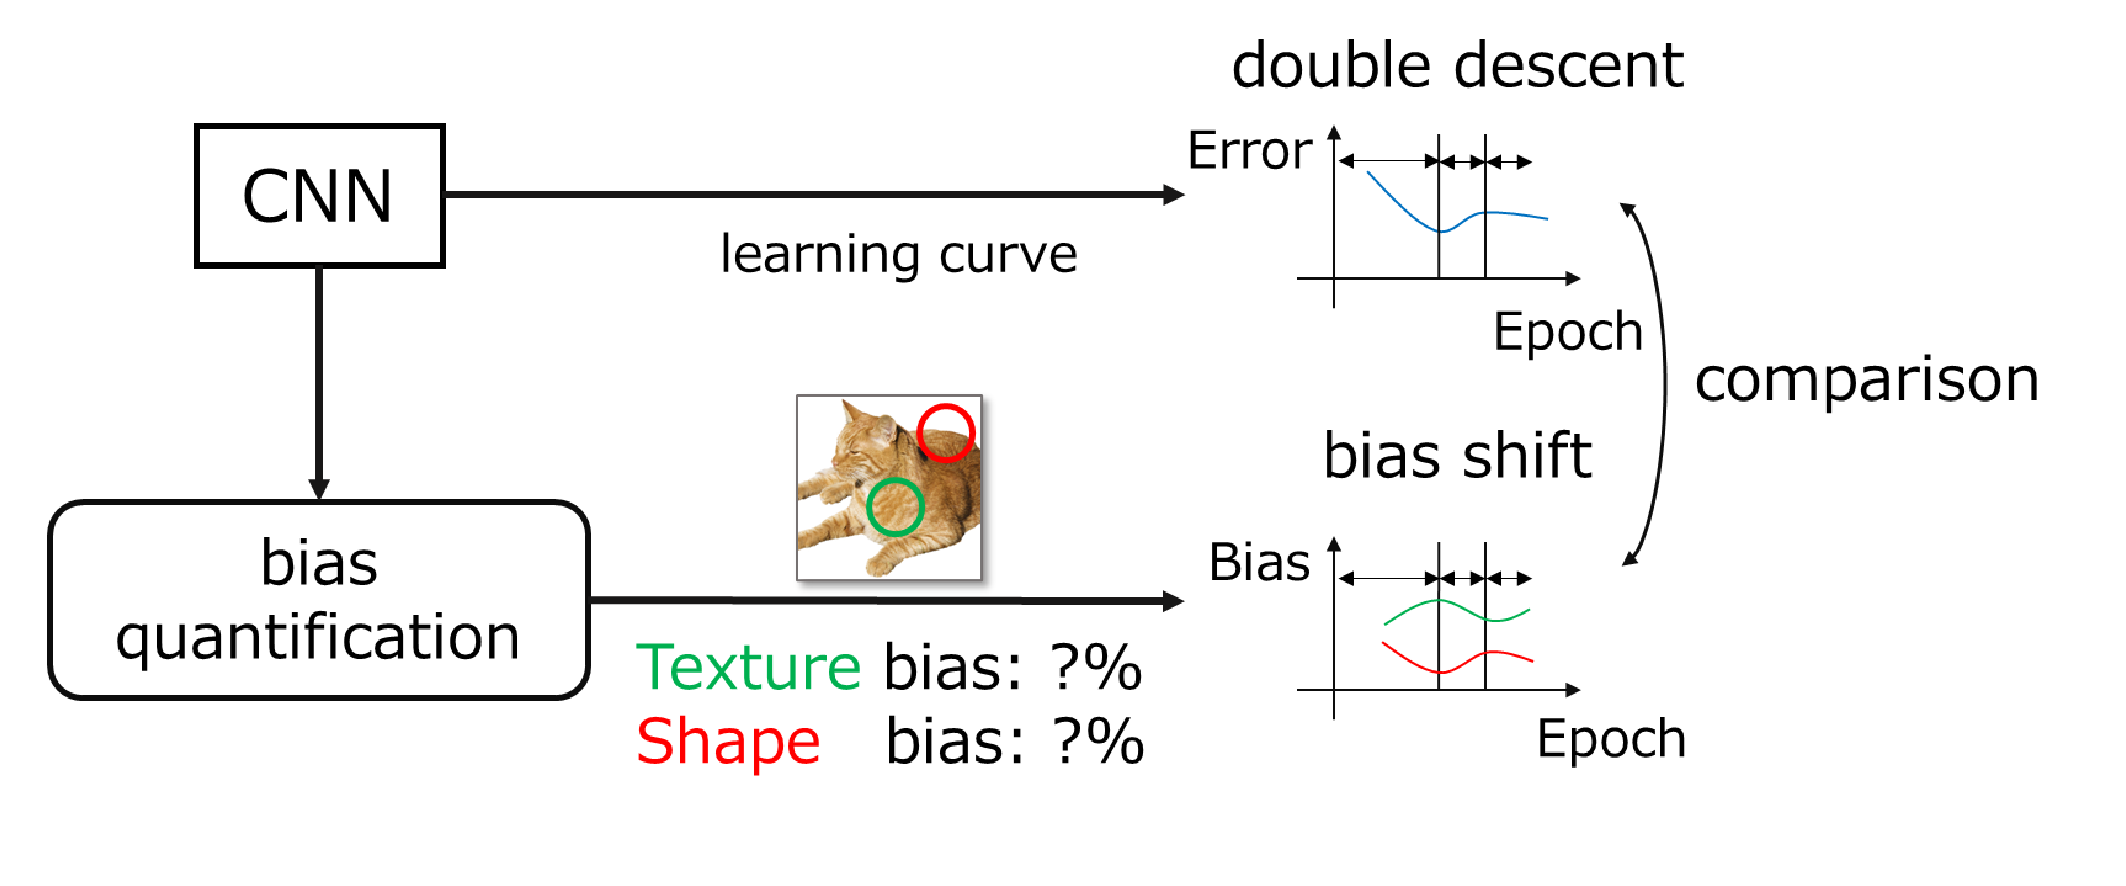
\includegraphics[width=1\columnwidth]{fig/fig1.pdf}
% \vspace{-40pt}
% \caption[ Flow of the analysis process comparing double descent with the learning process of image features.]{
% % 本稿で紹介する解析プロセスの流れ.我々は畳み込みニューラルネットワーク(CNN)を採用し,二重降下条件下で多様な画像認識タスクを訓練した.形状/テクスチャのバイアスとテストエラーの時間的変化を監視し,形状やテクスチャを解釈するモデルの能力を評価すると同時に,それらの相関関係を探った.
% %  Flow of the analysis process comparing double descent with the learning process of image features. We employed convolutional neural networks (CNNs) to train diverse image recognition tasks under double descent conditions. We monitored the temporal evolution of the shape/texture biases and test errors metrics assessing the capacity of the model to interpret shapes and textures while also exploring their correlation.
% }
% \label{fig:fig2}
% \end{figure}

\section{論文構成}
第1章「序論」では,深層学習の急速な発展とその多岐にわたる応用分野について概観し,特に画像認識分野における性能向上とその背景にある主要な技術的進展について述べた.さらに,深層ニューラルネットワーク(DNN)の高い性能を支える内部表現の獲得メカニズムに関する既存の理論的枠組みと,経験的に観測される挙動との間に見られるギャップを指摘し,本研究の対象とする課題の明確化を行った.最後に,DNNの学習プロセスにおける視覚的特徴の獲得順序や相互作用の解明が,モデルの透明性向上や学習効率の改善に寄与することを示し,本研究の目的と貢献点を述べた.\par
第2章「先行研究」では,深層学習における視覚的特徴の獲得の研究がどのように進展してきたかを概観し,特に,画像認識における形状とテクスチャの重要性に関する先行研究を紹介する.さらに,深層学習における重要な経験的に知られる二重降下現象に関する最近の研究成果を紹介し,深層学習の学習プロセスにおける特徴獲得のメカニズムに関する理論的知見と実験的結果を紹介する.\par
第3章「」では,深層学習における,視覚的特徴の獲得メカニズムを紐解くための実験設定を提案し,その設定の理由と目的と述べる.\par
第4章「実験」では,第4章に基づいて行った検証結果,各種パラメータが与える実験結果への影響について検証する.\par
第5章「考察」では,実験結果についての考察を行う.\par
第6章「結論」では,本研究を総括する.\par
第7章「今後の展望」では,本研究で得られた知見から今後の方向性を示す.\par
\newpage 
    
\chapter{先行研究}
\section{深層学習}
一般に,機械学習で使用されるモデルは決定木,サポートベクターマシン(SVM),ニューラルネットワークなどが存在する.決定木は得られた予測に対して,どの説明変数が影響したのかの判断が容易であり,説明可能性が高いことで知られている.
一方で,ニューラルネットワークは,パーセプトロンを筆頭に,層の増加やネットワークの複雑化が図られてきた.黎明期においては,非線形な問題をとけるように知見が盛り込まれたSVMや,生物が持つ視覚野の知見から提案されたネオコグニトロンなどの画期的な手法が提案されてきた.その中でも,ネオコグニトロンに端を発する,畳み込みニューラルネットワーク(CNN)は,LeNet\cite{LeNet}により,誤差逆伝播法が導入され,2010年代以降には,AlexNet\cite{AlexNet},VGGNet\cite{VGGNet},ResNet\cite{ResNet},と急速に進化を遂げてきた.
このような深層化されたニューラルネットワークは興味深い性質や振る舞いを示す.しかし,そのような性質がどのような機序によって引き起こされるかについての完全な合意はとられていない.

\section{二重降下現象}
機械学習において,モデルの性能はモデルの複雑性(例えば,パラメータ数)と深い関係があり,モデルのパラメータ数が不足することによるアンダーフィッティング(Underfitting)\cite{underfitting}や,過剰なパラメータによるオーバーフィッティング(Overfitting)\cite{overfitting}などの現象が知られている.モデルの複雑性が増すにつれて,初めは性能が向上し(アンダーフィッティングを克服),その後過剰な複雑性により性能が低下するとされていた.これはU字型のカーブ,いわゆるバイアス-バリアンス トレードオフ\cite{Rajnarayan2010}として知られている.

ところが近年発見されたDouble Descent\cite{Belkin_2019}と呼ばれている現象は,モデルの複雑性がさらに増すと,性能が再び向上する.つまり,最初のU字型のカーブ(アンダーフィッティングからオーバーフィッティングへの移行)の後,さらに複雑性が増加すると,新たな性能向上のフェーズが現れるのである.過剰パラメータを持つディープニューラルネットワークが,理論的にはオーバーフィッティングを起こすべきなのに,実際には優れた汎化性能を示す場合がある\cite{ResNet,ViT}.

このDouble Descentは,Belkinら\cite{Belkin_2019}によって決定木や二層のニューラルネットワークで確認され,その後,Nakkiranら\cite{nakkiran2021deep}が,ディープニューラルネットワーク(DNN)においても観察されること,学習エポック数の増加に対してもDouble Descentが起こることを示した.さらに,パラメータの枝刈りによるスパース性の増加に対してもDouble Descentが起こることが報告されている\cite{He}.パラメータ数,学習エポック数,スパース性の増加に伴って観察されるDouble Descentは,それぞれ,Model-wise Double Descent,Epoch-wise Double Descent,Sparse Double Descent と呼ばれている\cite{nakkiran2021deep,He}.

\section{画像認識における形状・テクスチャ}
Geirhosらは,ImageNetで学習したCNNが,分類のために特に画像のテクスチャを重視することを示した~\cite{Geirhos}.彼らは,相反する形状とテクスチャ情報を持つ画像をCNNに入力し,出力が形状ベースのラベルとテクスチャベースのラベルのどちらに一致するかをチェックした.この結果に基づいて,CNNが認識において形状とテクスチャのどちらを優先するかを分析した.一方,Islamらは,ニューロンの潜在表現に基づくモデルにおいて,形状とテクスチャのどちらを重視するかを定量的に判断する方法を提案した~\cite{Islam}.この方法によって,CNNがどの特徴に偏重するのかを定量的に分析することができる.さらに,Geらは人間の視覚系のモデル化を試み,Human Vision System (HVS)を開発した.HVSは,画像分類時にどの特徴(形状,テクスチャ,色など)が最も重要な役割を果たすかを定量的に評価可能である\cite{Ge}.

\section{画像認識における二重降下現象と形状・テクスチャバイアスの関係}

\begin{figure}[t]
    \centering
    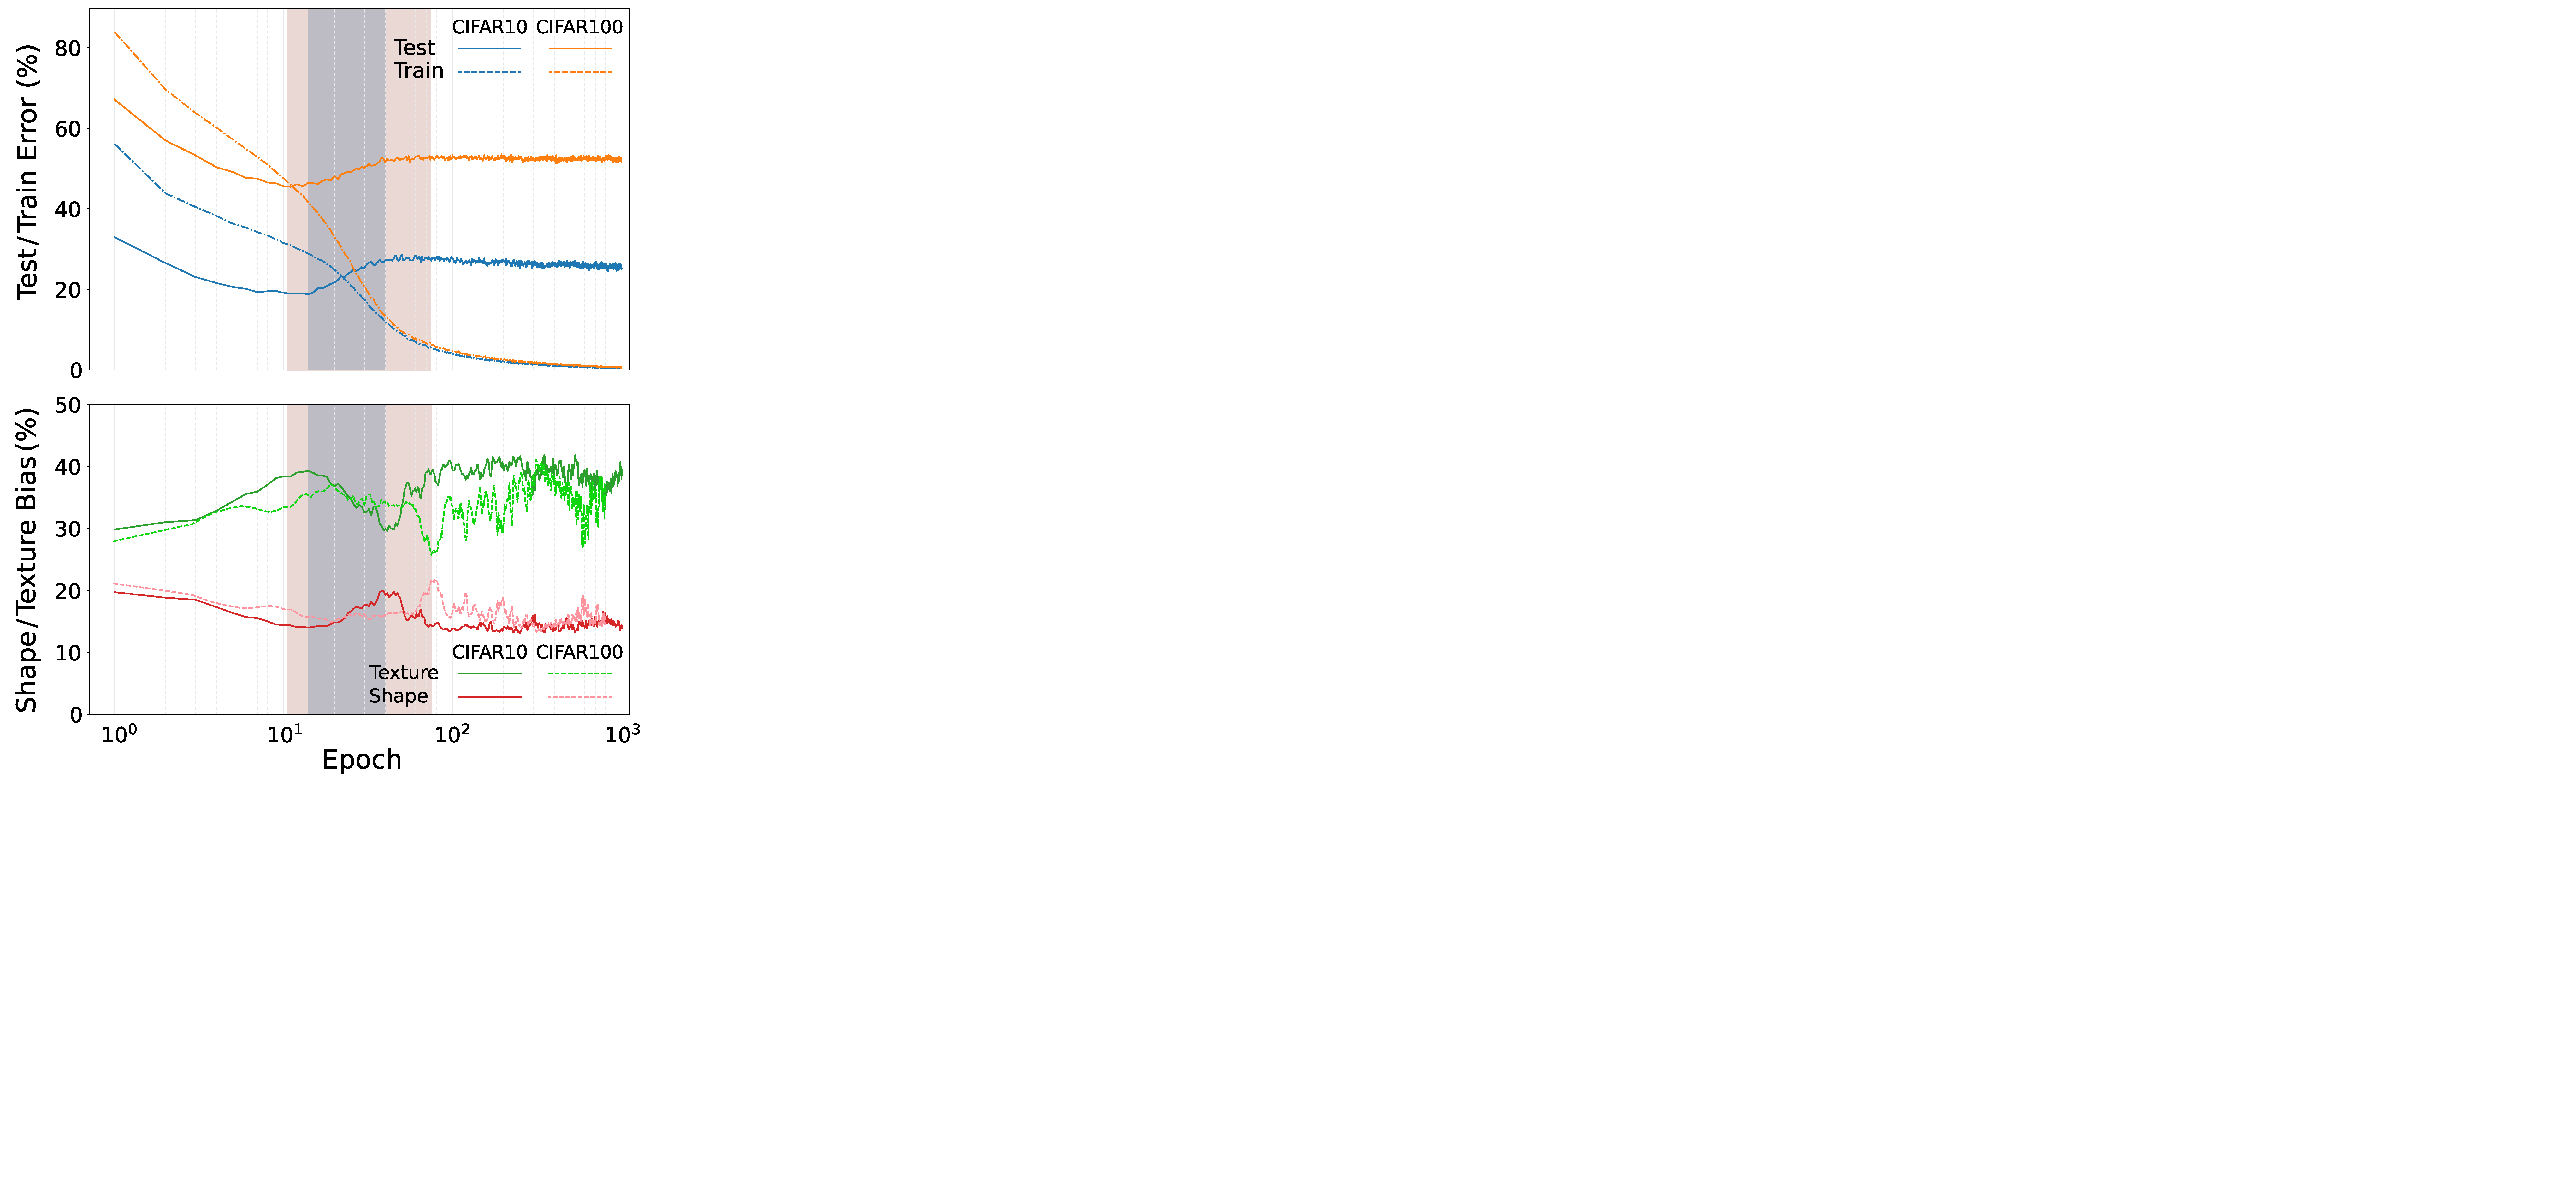
\includegraphics[width=\linewidth]{fig/iwaseICPR.pdf}
    \caption[ResNet18の学習過程における二重降下現象と形状・テクスチャバイアスの変化の同期性.]{ResNet18の学習過程における二重降下現象と形状・テクスチャバイアスの変化の同期性.ImageNetで事前学習済みのResNet18を使用し,CIFAR-10とCIFAR-100の学習を行った際のテストエラー率.また,それぞれのエポックでのモデルにおける形状・テクスチャバイアスを計算した結果.
    二重降下現象を3つのフェーズに分けた際に,第1フェーズでは,テストエラー率が減少するときにはテキスチャバイアスが強くなる.次に過学習のタイミングで形状バイアスが強くなり,再度はエラー率が下がるときテクスチャバイアスを強くするように戻る.}
    \label{fig:iwaseICPR}
\end{figure}
\UTF{9AD9}橋らの研究\cite{DD_STB}は,画像認識タスクにおける二重降下現象と,CNNの形状バイアスおよびテクスチャバイアスの変化の関連性を示唆した.この研究では,二重降下現象と形状・テクスチャバイアスの変化のタイミングに相関が見られ,テスト誤り率が上昇から下降に転じるタイミングと,形状バイアスが増加し始めるタイミングが一致することが示された.
また,事前学習の有無による学習過程の違いも観測された.事前学習ありのモデルでは初期からテクスチャバイアスが高く,学習が進むと形状バイアスが増加する傾向が見られた.一方,事前学習なしのモデルでは学習初期は形状バイアスが高く,その後テクスチャバイアスが増加する傾向が確認された.

岩瀬らの研究~\cite{icpr2024iwase}では,さらに形状・テクスチャバイアスと二重降下現象に関する同期性を様々な角度から検証している.この研究では,CIFAR-10とResNet18の組み合わせ以外の条件下で同期性が確認されたほか,どの層が要因となり,同期性が起こっているのかが明らかとなった.
これらの知見は,画像認識モデルの学習ダイナミクスと二重降下現象の関係性に新たな洞察を提供している.
この同期性を図\ref{fig:iwaseICPR}に示す.
これまでの研究では,CNNの学習過程における形状とテクスチャという特徴の獲得と二重降下現象の関係について研究されてきた.そこで,本研究では形状とテクスチャではなく,色と数字という概念を設定し,2つの学習過程における概念獲得の過程の観測した.
\newpage

% \chapter{深層学習における二重降下現象}
\section{はじめに}
本研究では,深層学習における二重降下現象を観察するためにNakkiranら\cite{nakkiran2021deep}の条件を使用している.本章では,学習時における具体的な実験設定を述べるとともに,その条件を使用したModel-wise Double Descent, Epoch-wise Double Descentの追試結果を示す.

\section{Nakkiran's setting}
\label{sec:Nakkiran's setting}
% PyTorchで利用可能なImageNetで事前学習された重みを持つResNet18を使用し,CIFAR-10~\cite{Krizhevsky2009_cifar}で学習させる.学習データにはラベルノイズとデータ拡張を加える.ラベルノイズは,学習データの正しいラベルを$p$の確率でランダムに別のラベルに変更する.データ補強では,画像の上下左右に4ピクセルのマージンを加え,32x32のサイズにトリミングし,画像をランダムに水平反転させる.バッチサイズを128に設定し,損失関数としてCrossEntropyLossを用いる.最適化にはAdam~\cite{Adam}を用い,学習率は0.0001とする.
ResNet18を使用し,CIFAR-10~\cite{Krizhevsky2009_cifar}を学習させる.学習データにはラベルノイズとデータ拡張を加える.ラベルノイズは,学習データの正しいラベルを$p$の確率でランダムに別のラベルに変更する.データ補強では,画像の上下左右に4ピクセルのマージンを加え,32x32のサイズにトリミングし,画像をランダムに水平反転させる.バッチサイズを128に設定し,損失関数としてCrossEntropyLossを用いる.最適化にはAdam~\cite{Adam}を用い,学習率は0.0001とする.

\subsection{Model-wise Double Descent}
一般的なResNet18の各ブロックの出力チャネル数が[64, 128, 256, 512]であるのに対し,[1$\times k$, 2$\times k$, 3$\times k$, 4$\times k$]と横幅を可変にすることでパラメータ数を制御し二重降下を観察している.以降横幅可変なResNet18をResNet18kと呼称する.ラベルノイズは$p=0.15$として,$k=1\sim64$に設定したResNet18kをそれぞれ4,000 epoch学習させ,最終的なテスト誤り率をグラフに図示する.実際の結果を\cref{fig:DD}に示す.$k=5$,$k=10$の付近でテスト誤り率が下降から上昇,上層から下降と切り替わり,二重降下の曲線が観察できる.

\begin{figure}[ht]
    \centering
    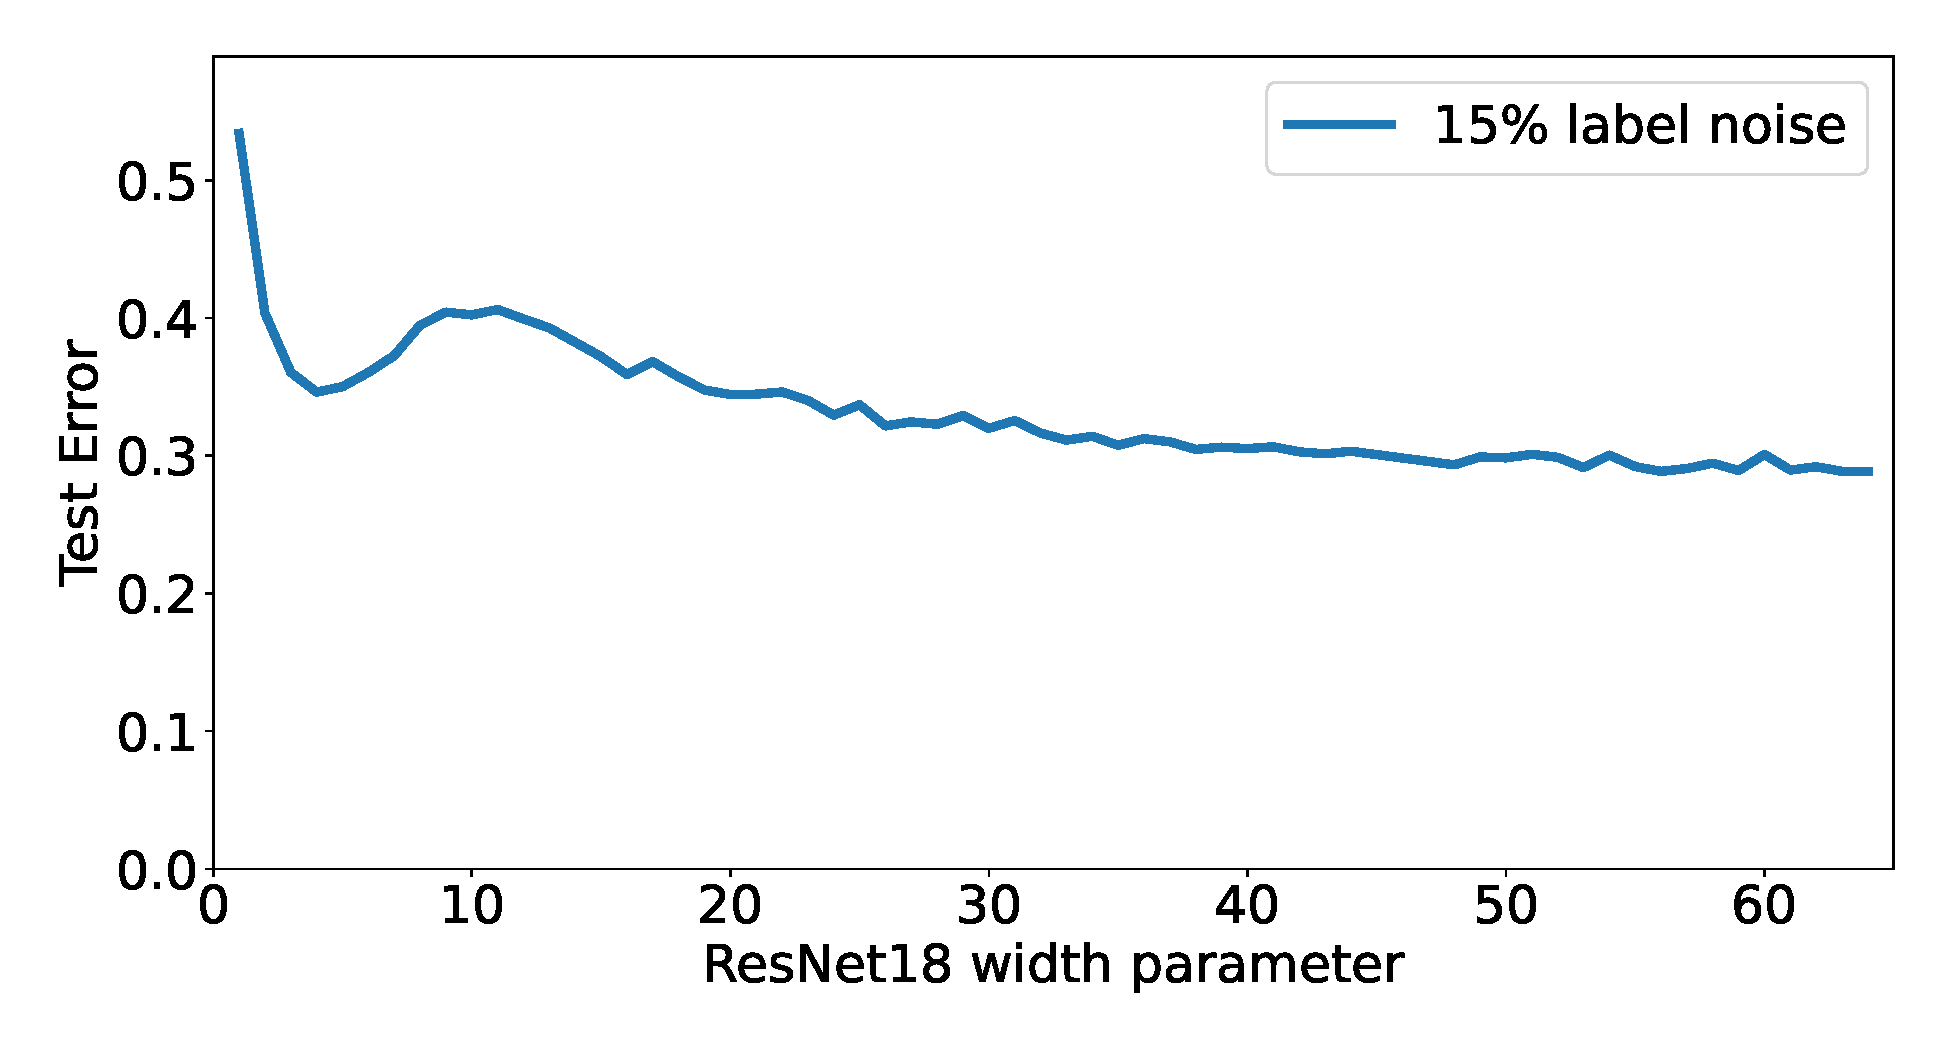
\includegraphics[width=1\columnwidth]{fig/DoubleDescent.pdf}
    \caption{Model-wise Double Descent by Nakkiran's setting}
    \label{fig:DD}
\end{figure}

\newpage

\subsection{Epoch-wise Double Descent}
先述した,ResNet18kを$k=128$で使用し,同様に4,000epoch学習させ,学習過程のテスト誤り率の推移を観察する.実際の結果を\cref{fig:EDD}に示す.20から30epoch目,60から70epoch目付近でテスト誤り率が下降から上昇,上層から下降と切り替わり,二重降下の曲線が観察できる.

以降の実験では,一般的なResNet18($k=64$に設定したResNet18kとほぼ同等)を先述した条件で学習,学習過程における二重降下を観察している.

\begin{figure}[ht]
    \centering
    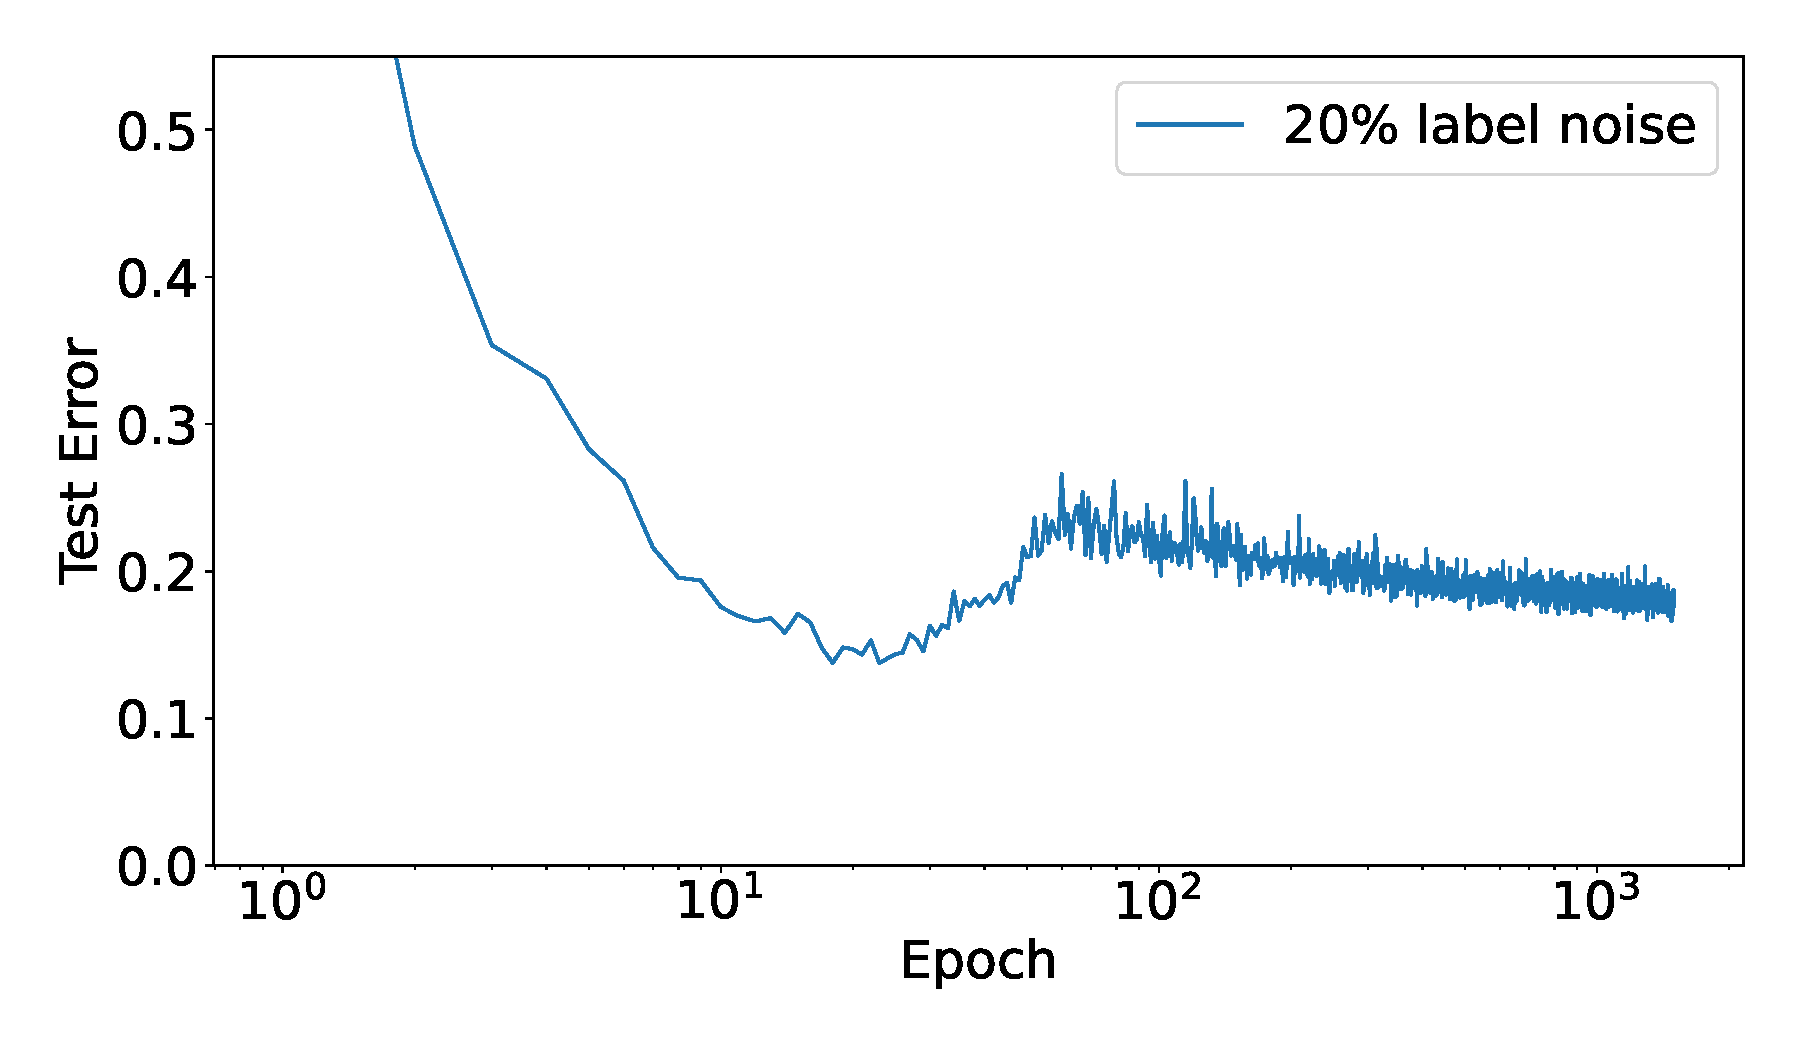
\includegraphics[width=1\columnwidth]{fig/Epoch-wise_DoubleDescent.pdf}
    \caption{Epoch-wise Double Descent by Nakkiran's setting}
    \label{fig:EDD}
\end{figure}

\newpage

% \chapter{自然画像が持つ特徴に着目した分析}
\section{概要}
本章では,深層学習におけるEpoch-wise Double Descentと自然画像が持つ形状・テクスチャ特徴との関係を調査する方法を説明する.\cref{fig:fig2}はこの方法の概要を示している.まず,二重降下が起きる条件でCNNを学習し,学習曲線の推移を観察する.さらに,各エポックの形状・テクスチャ偏重度をIslamらの方法により定量化し,学習過程での推移を同様に観察する.このようにして,二重降下の推移と偏重度の推移を比較する.さらに定量的な評価を行うために,二重降下を三つのフェーズに分け,各フェーズでのテスト誤り率と形状・テクスチャ偏重度との相関係数を評価する.以降ではEpoch-wise Double Descentの観察方法,二重降下の各フェーズの分割方法,形状・テクスチャ偏重度の算出方法についてそれぞれ説明する.
\section{二重降下現象のフェーズ分割}
\label{sec:Phase division of double descent} 
本研究では,二重降下とモデルの形状テクスチャの偏りとの関係を分析するために,二重降下におけるテスト誤差の推移に基づいて以下の3つのフェーズに分割する.
\textbf{Phase1}: 学習開始からテスト誤差が最小になるまで.
\textbf{Phase2}: Phase1が終了してから,テスト誤差が再び減少するまで.
\textbf{Phase3}: Phase2が終了してから,以降の区間.

これらのフェーズを決定するために,勾配ベースの方法を利用する.具体的には,エポック間のテスト誤り率を監視し,連続するエポック間の差$\Delta e$ を $\Delta e=\left|e_i-e_{i+5}\right|$として計算する.任意のエポックiにおいて,差$\Delta e$が指定された閾値θ以下であれば,テスト誤差は安定しているか,わずかに改善されている.このときの最小エポック番号までの区間を「Phase1」と定義する.`Phase2'については,`Phase1'の直後のエポック番号から,差が$\theta$以下となる最小のエポックまでの区間とする.`Phase3'は,`Phase2'以降の区間を示す.実験では,閾値$\theta$は0.1に設定した.使用した実験セットアップでは,経験的に二重降下の二回目の降下は一回目の降下より低いテスト誤り率を持たないため,フェーズは上記のプロセスで分割可能である.

\section{形状・テクスチャ偏重度の定量化}
\label{sec:形状・テクスチャ偏重度の定量化}
我々は,CNNの最終畳み込み層における形状・テクスチャ特徴を符号化するニューロン数(=次元数)をIslamらの方法\cite{Islam}によって推定し,その割合をモデルが持つ形状・テクスチャ偏重度と定義する.
次元の推定には,Islamらのプログラム\footnote{https://github.com/islamamirul/shape\_texture\_neuron}を使用した.
形状・テクスチャ偏重度を計算するフローを\cref{fig:fig3}に示す.

\begin{figure}[t]
\centering
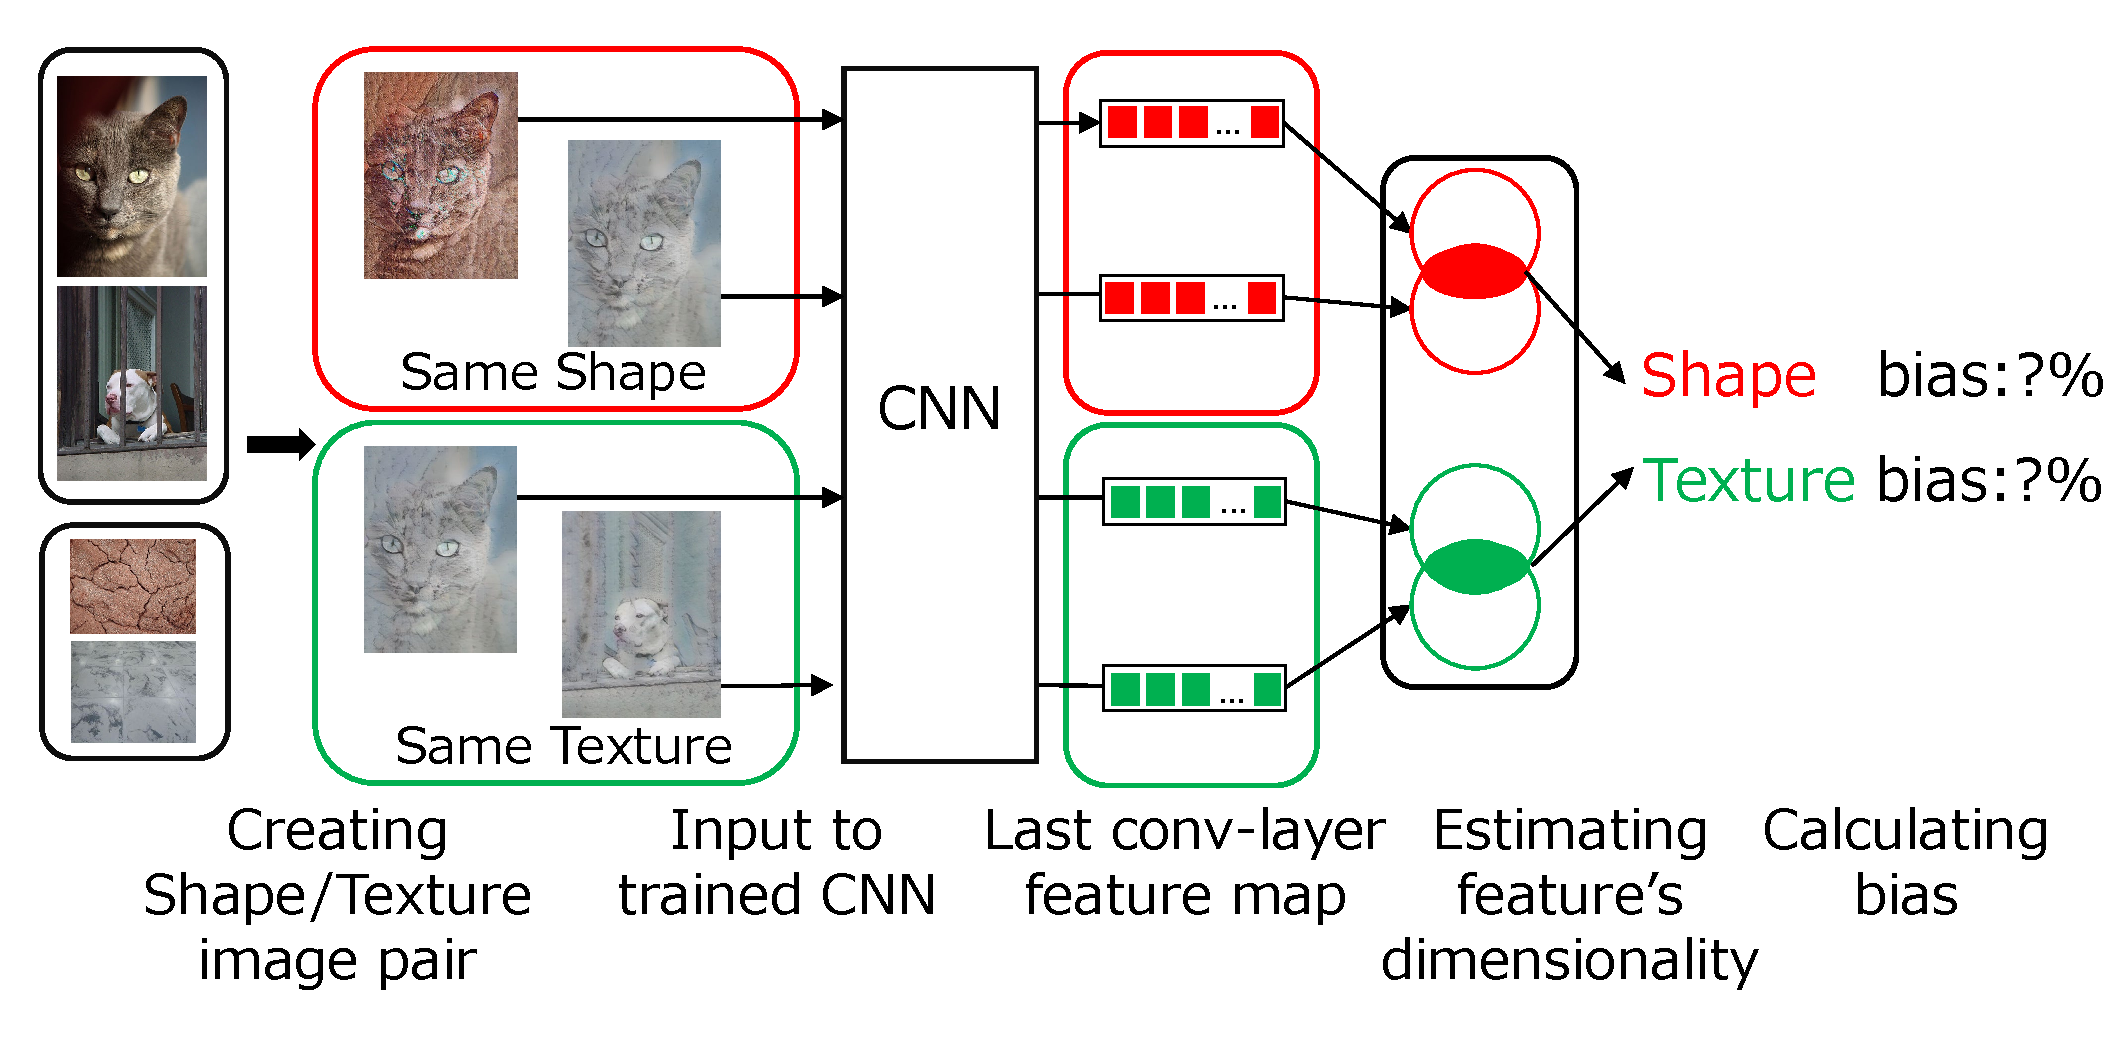
\includegraphics[width=1\columnwidth]{fig/fig2.pdf}
\caption{
%図3.Islamの方法の概要.この図は,[14]の方法で形状とテクスチャの重み付けを計算するプロセスの概要を示しています.
% CNNの学習過程における形状・テクスチャ情報の働きを解析するためのIslamの方法\cite{Islam}.
%Islamの方法の概要.この図は,[14]の方法で形状とテクスチャの重み付けを計算するプロセスの概要を示しています.
Overview of the process of calculating the shape/texture bias using the method of \cite{Islam}.
}
\label{fig:fig3}
\end{figure}

形状・テクスチャ偏重度の定量化に使用するデータセットの作成方法について述べる.この目的のために,PASCAL VOC 2012データセット~\cite{pascal-voc-2012} とDescribable Textures Dataset~\cite{cimpoi14describing}を用いる.PASCAL VOC 2012データセットからは,単一のオブジェクトを含む画像のみを選択し,Describable Textures Datasetからは,ランダムに5つのテクスチャ画像を選択する.Describable Textures Datasetから選択されたテクスチャ画像をスタイルとして使用し,PASCAL VOC 2012データセットから選択されたすべての画像に対してスタイル変換を実行する.このスタイル転送には,AdaIn transferアルゴリズム~\cite{AdaIn}を利用する.このようにして作成されたデータセットをStylized PASCAL VOC 2012(SVOC)と呼ぶ.

SVOCを用いて偏重度を定量化する方法について詳しく説明する.SVOCを使うことで,共通の形状特徴を持つ画像ペアと共通のテクスチャ特徴を持つ画像ペアをサンプリングすることができる.これらのペアを定量化したいCNNモデルに入力すると,最終的な畳み込み層のニューロンから両方の共通特徴セットに対する特徴マップペアが得られる.これらの特徴マップを用いて,以下の式から各特徴の相関係数を計算し,偏重度を求める.

実際の計算過程を述べる.形状情報が共通する画像ペアを入力して$i$番目のニューロンから得られる特徴マップペアを$z^a_i, z^b_i$ とする.それら特徴マップペアから相関係数を計算,計算された相関係数を$\rho_i^{shape}$とする.同様に同様に,テクスチャ情報が共通する画像ペアを入力し,出力される特徴ベクトルのペアから$\rho_i^{texture}$を求める.
そして,ニューロンのごとの$\rho_i^{shape}$,$\rho_i^{texture}$それぞれの総和,形状とテクスチャのとベースライン値($=ニューロン数|z|$)から,ソフトマックス関数を用いて形状とテクスチャの偏重度を決定する.

この方法は,$i$番目のニューロンがある概念(例えば形状)をエンコードしている場合に,形状情報共通した画像ペアを入力すると,$z^a_i, z^b_i$の相互情報量は高くなり,相互情報量は(1)の式のように相関係数から下界が求まることから,相関係数を用いて計算される.

\begin{align}
\operatorname{MI}\left(z_i^a, z_i^b\right) \geq-\frac{1}{2} \log \left(1-\rho_i^2\right), \quad \text { where } \rho_i=\frac{\operatorname{Cov}\left(z_i^a, z_i^b\right)}{\sqrt{\operatorname{Var}\left(z_i^a\right) \operatorname{Var}\left(z_i^b\right)}}
\end{align}

Islamらの実装では,論文内における説明とは異なり,高速化のため,ニューロンごとに$\rho_i^{shape}$,$\rho_i^{texture}$を計算していないことに注意が必要である.
    
\newpage

% \chapter{実験}
\section{はじめに}

本節では,二重降下と形状・テクスチャ特徴との関係を検証するため,以下の検証を行う:(1)先行研究においてEpoch-wise Double Descentを確認した設定を参考に,テスト誤り率,形状・テクスチャ偏重度それぞれの推移を比較する.また,\cref{sec:Phase division of double descent}で定義したそれぞれのPhaseにおいて,どの程度相関があるかを定量的に調べる. (2)(1)に基づき,二重降下とテクスチャ・形状の偏りの関係の理解を深めるために,詳細なアブレーション実験を行う.本章の実験で使用している学習プログラムは,付録\ref{学習プログラム}に記載する.

\section[Nakkiran's setting result]{Nakkiran's setting result (\cref{fig:overview})}

Nakkiran~\cite{nakkiran2021deep}の実験設定(\cref{sec:Nakkiran's setting})を参考に,テスト誤り率,形状・テクスチャ偏重度それぞれの推移の比較を行った.二重降下とモデルの形状・テクスチャ偏重度を比較した結果を\cref{fig:overview}に示す.青い線はテスト誤差の二重降下の推移を,赤い線はモデルの形状偏重度の推移を,緑の線はテクスチャ偏重度の推移を表している.形状・テクスチャ偏重度の推移においては,変動におけるノイズの軽減のために,5項移動平均を取っていることにテスト誤り率,形状偏重度それぞれの推移を比較すると,Phase 1では下降し,Phase 2では上昇,Phase 3では再度下降するといった相関がみられた.また,テスト誤り率とテクスチャ偏重度には逆の相関がみられている.

\begin{figure}[h]
% \hspace{-25pt}
\centering
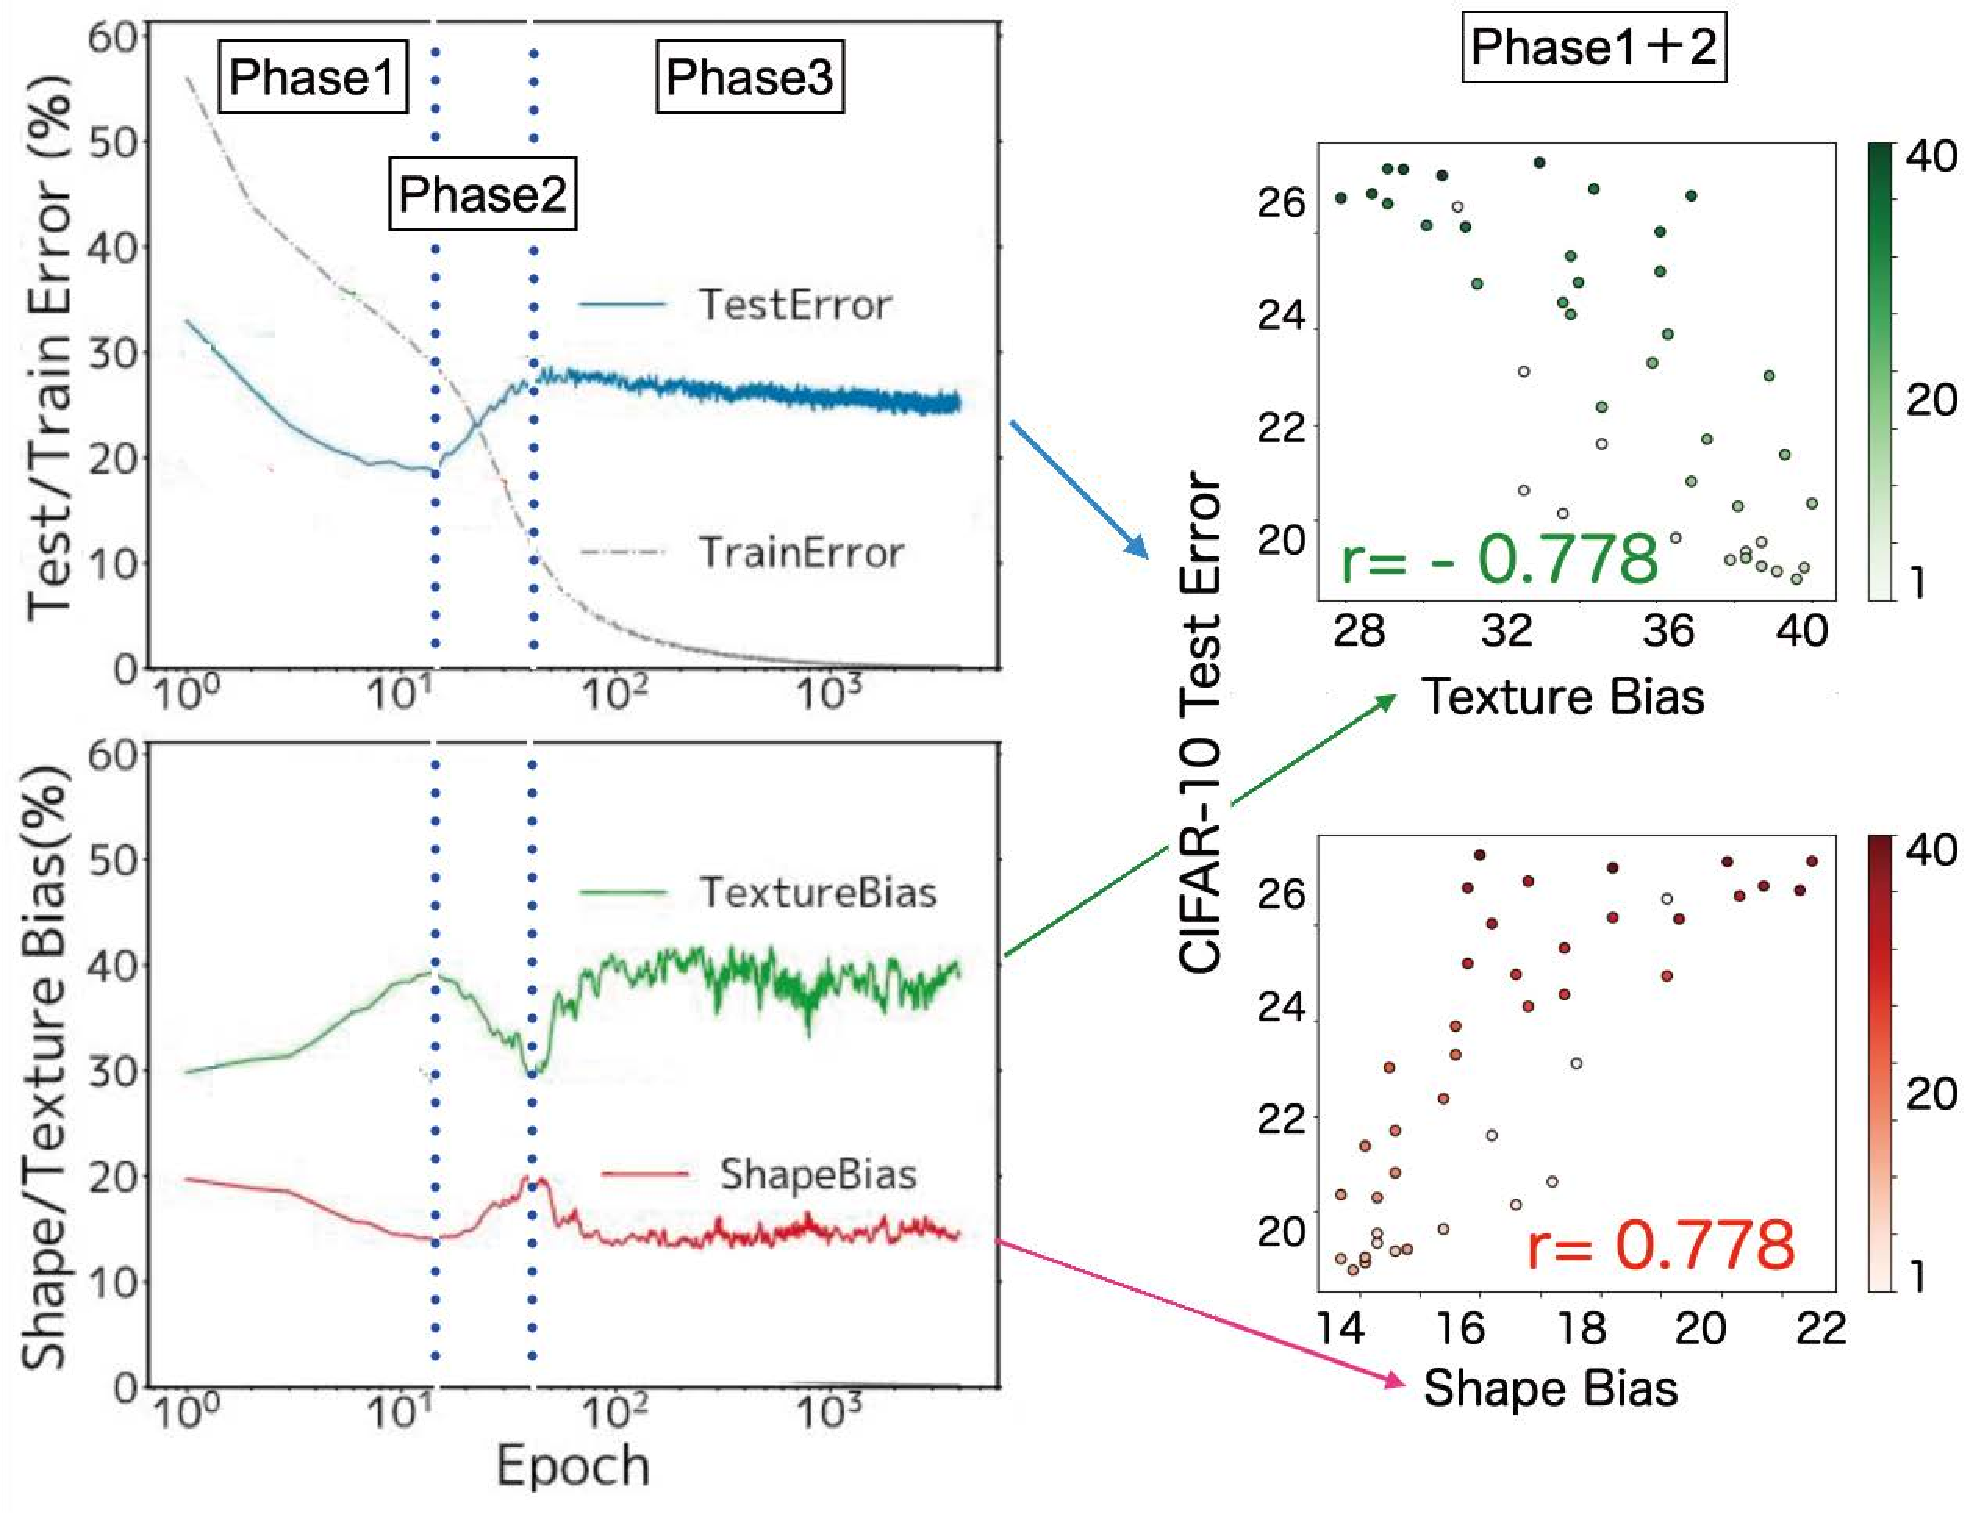
\includegraphics[width=1.0\columnwidth]{fig/result_overview.pdf}
\caption[Schematic overview of this study.]{
% 図2.本研究の概要を示す模式図.左上: 二重降下(DD)が観測されたCIFAR-10画像認識タスクの学習曲線;テスト誤差はその時間的分化に基づいて3つのPhaseに分けられた.実験結果はnakiranらによる既報[18]と同条件でDDを再現した結果である.左下: 前述の学習過程におけるモデルの形状/テクスチャの偏りを記録したもの.テスト誤差と形状・テクスチャの偏りの同期的変化を示す.右: テストエラーと形状/テクスチャバイアスの散布図.特にPhase 1とPhase 2において,テストエラーと形状バイアスの間には正の相関があり,テストエラーとテクスチャバイアスの間には負の相関がある.
Schematic overview of this study. Top left: Learning curve of the CIFAR-10 image recognition task where double descent was observed; test errors were divided into three phases based on their temporal differentiation. The experimental results are a reproduction of double descent under the same conditions as previously reported by Nakiran \textit{et al.}\cite{nakkiran2021deep}. Bottom left: This records the model's shape/texture bias during the aforementioned learning process. It shows the synchronous changes between test errors and shape/texture biases. Right: A scatter plot of test error and shape/texture bias. Especially in Phase 1 and Phase 2, there is a positive correlation between test error and shape bias, and a negative correlation between test error and texture bias.
% Schematic illustration showing the outline of this study.Top left: Learning curve depicting the CIFAR-10 image recognition task with observed double descent (DD); the test error was divided into three phases based on its temporal differentiation.The experimental results are the results of reproducing DD under the same conditions as in the previous report by nakiran \textit{et al.}\cite{nakkiran2021deep}.Bottom left: Recorded shape/texture biases of the model during the aforementioned learning process.Observations indicate synchronous changes in test error and shape/texture biases.Right: Scatter plot representing test error and shape/texture bias values for the interval encompassing phases 1 and 2, revealing a positive correlation between test error and shape bias, as well as a negative correlation between test error and texture bias.
}
\label{fig:overview}
\end{figure}

\newpage

\section[Correlation analysis in each phase of the double descent]{
Correlation analysis in each phase of the double descent (\cref{tab:base_condition_result})
}
4.3節で定義したPhase1,Phase2,Phase3におけるテスト誤り率と形状・テクスチャ偏重度の相関係数を計算し,より詳細な評価を行った.これらの結果を\cref{tab:base_condition_result}に示す.Phase1とPhase2におけるテスト誤り率と形状偏重度との相関係数はそれぞれ0.898と0.771であり,正の相関があることがわかる.逆に,Phase1とPhase2におけるテスト誤り率とテクスチャ偏重度との相関係数は\textminus0.829と\textminus0.797であり,負の相関を示している.Phase3では,形状偏重度の相関値は\textminus0.026,テクスチャ偏重度の相関値は0.118であり,相関は見られなかった.これらの結果から,Phase1と2では相関が見られたが,Phase3では相関が見られなかった.形状とテクスチャの関係を簡単に理解するために,形状とテクスチャの相関値をScoreと呼ばれる指標で表す.Scoreは,これらの相関係数の絶対値の平均である.Scoreが高いほど,テスト誤り率と形状/テクスチャ偏重度それぞれとの相関が強いことを示す.以降の実験では,今回の条件において高い相関を示したPhase1,2とPhase3それぞれの区間で相関係数とScoreを算出し,定性的な分析に利用する.

\begin{table}[h]
\centering
    \caption[The correlation coefficients and scores for the three phases]{
    % 定義した方法(\cref{sec:Phase division of double descent})によって分けた3つのPhaseの相関係数とスコア.相関係数を計算するために使用された実際のデータ間隔(Epoch range),Test ErrorとShape biasから計算された相関係数,Test ErrorとTexture biasから計算された相関係数,2つの相関係数から計算された相関スコアを示している.
    The correlation coefficients and scores for the three phases divided according to the method defined in (\cref{sec:Phase division of double descent}). It shows the Epoch range used to calculate the correlation coefficients, the correlation coefficients calculated from Test Error and Shape bias, the correlation coefficients calculated from Test Error and Texture bias, and the correlation score computed from these two correlation coefficients.
    % Correlation coefficients and scores for the three phases, divided by \cref{sec:Phase division of double descent}. The following table shows the actual data interval used to compute the correlation coefficients (Epoch range), the correlation coefficient computed from the Test Error and the Shape corr, the correlation coefficient computed from the Test Error and the Texture corr, and the correlation score computed from the two correlation coefficients.score calculated from the two correlation coefficients.
    }
    
    \scalebox{1.2}{
    \begin{tabular}{c|c|SS|c}
    \toprule[0.8pt]
     Phase & Epoch range & {Shape corr}& {Texture corr}& Score\\
     \midrule[0.5pt]
    Phase1 & 2 - 12 &0.898 &-0.829 &0.863\\
    Phase2 & 12 - 41&0.771& -0.797&0.784\\
    Phase3 & 41 - 1,000&-0.026 & 0.118&0.072\\
    \toprule[0.8pt]
    \end{tabular}
    }
    \label{tab:base_condition_result}
    % \vspace{-15pt}
\end{table}

\newpage

\section{詳細なアブレーション実験}
\subsection{概要}
本節では,先に述べた条件から一部を変更し,実験を構成する各条件が二重降下と偏重度の推移にどのように影響を与えるかを検証する.具体的には,以下の条件を変更した: "事前学習の有無","使用データセット","ResNet Family内でのモデル変更","使用CNNモデル","バッチサイズ","ラベルノイズの割合","シード値".実際に変更した条件と該当する図の一覧を\cref{tab:ablation_list}に示す.以降の実験では,実験の高速化のために,学習回数を1,000 epochとした.

\begin{table}[h]
\centering
    \caption[List of changed conditions and corresponding fig. numbers in ablation studys.]{List of changed conditions and corresponding fig. numbers in ablation studys.This table shows only the conditions changed from the base in bold.Blank spaces indicate the same as above.}
    \scalebox{1.1}{
    \begin{tabular}{c|c|c|c|c|c|c}
    \toprule[0.8pt]
    pre-train & Model & dataset & batchsize & Label Noise & seed & Fig. No\\
     \midrule[0.5pt]
    ImageNet & ResNet18 & CIFAT-10 & 128 & 0.2 & 42 & \ref{fig:overview}\\
    \midrule[0.1pt]
    \textbf{None}& ResNet18 & CIFAT-10 & 128 & 0,2 & 42 & \ref{fig:comp_INSR}\\
    ImageNet &          & \textbf{CIFAT-100}&     &     &    & \ref{fig:comp_IN_dataset}\\
             &\textbf{ResNet34} & CIFAT-10 &     &     &    & \ref{fig:comp_model}\\
             &\textbf{ResNet50} &          &     &     &    & \ref{fig:comp_model}\\
             &\textbf{DenceNet} &          &     &     &    & \ref{fig:comp_cnn_model}\\
             &\textbf{MobileNet}&          &     &     &    & \ref{fig:comp_cnn_model}\\
             &\textbf{EfficientNet}&       &     &     &    & \ref{fig:comp_cnn_model}\\
             & ResNet18 &          &  \textbf{8} &     &    & \ref{fig:comp_batchsize}\\
             &          &          &  \textbf{16} &     &    & \ref{fig:comp_batchsize}\\
             &          &          &  \textbf{64} &     &    & \ref{fig:comp_batchsize}\\
             &          &          & 128 & \textbf{0.4} &    & \ref{fig:comp_ln}\\
             &          &          &     & \textbf{0.6} &    & \ref{fig:comp_ln}\\
             &          &          &     & 0.2 &  \textbf{0} & \ref{fig:comp_seed}\\
             &          &          &     &     &  \textbf{1} & \ref{fig:comp_seed}\\
    \toprule[0.8pt]
    \end{tabular}
    }
    \label{tab:ablation_list}
\end{table}

\newpage

\subsection[Init parameter]{Init parameter (see \cref{fig:comp_INSR})}
ベースラインの条件では,先行研究において,ImageNetにおける学習の文脈で形状・テクスチャに関する研究が行われていたことを考慮し,ImageNet-1kの学習済みパラメータをモデルの初期値として用いた.本実験では,ImageNet-1kとランダム値(Scratch)を比較することで,初期値に基づく形状とテクスチャの偏りの関係を検証した.その結果を\cref{fig:comp_INSR}に示す.この結果から,ImageNet-1kの初期パラメータを用いた場合,形状・テクスチャ偏重度が明瞭に変化することがわかる.このような結果になった理由の1つとして,ImageNetを事前学習することで得られる特徴表現と,CIFAR-10を学習することで得られる特徴表現が大きく異なることが考えられる.それによって,ImageNetを事前学習したパラメータの状態から,CIFAR-10に適応するために,大きくパラメータの状態が変化し,その結果偏重度の推移の変化として現れたと考えられる.また,Scratchを用いた場合においても,二重降下のPhase 1からPhase 2への移り変わりにおいて,特にテクスチャ偏重度はわずかながら上昇から下降に転じているように見受けられる.そのため,双方の条件において,学習傾向の移り変わりが起きている可能性が考えられる.しかし,CIFAR-10の学習時に,ImageNetで事前学習した場合に,二重降下と同期したような挙動を強くすることは,非常に興味深い現象である.このような差異について,パラメータが如何に変化していっているかという点が重要であると考えられる.
% ベースラインの条件では,先行研究において,ImageNetにおける学習の文脈で形状・テクスチャに関する研究が行われていたことを考慮し,ImageNet-1kの学習済みパラメータをモデルの初期値として用いた.本実験では,ImageNet-1kとランダム値(Scratch)を比較することで,初期値に基づく形状とテクスチャの偏りの関係を検証した.その結果を\cref{fig:comp_INSR}に示す.この結果から,ImageNet-1kの初期パラメータを用いた場合,形状・テクスチャ偏重度が明瞭に変化することがわかる.しかし,Scratchを用いると,特徴的な変化は生じない.このような結果になった理由の1つとして,ImageNetを事前学習することで得られる特徴表現と,CIFAR-10を学習することで得られる特徴表現が大きく異なることが考えられる.それによって,ImageNetを事前学習したパラメータの状態から,CIFAR-10に適応するために,大きくパラメータの状態が変化し,その結果偏重度の推移の変化として現れたと考えられる.しかし,CIFAR-10の学習時に,ImageNetで事前学習した場合だけ,偏重度が一定で推移せず,二重降下と同期したような挙動をすることは,非常に興味深い現象である.
% 本実験では,ImageNetで事前学習した場合とランダム値(Scratch)を比較することで,初期値に基づく形状とテクスチャの偏りの関係を調べた.その結果を\cref{fig:comp_INSR}に示す.この結果から,ImageNetで事前学習した場合に限って,形状・テクスチャ偏重度が特異に変化することがわかる.しかし,Scratchを用いると,特徴的な変化は生じない.このような結果になった理由の1つとして,事前学習で得た特徴から新たなデータに適合するににあたって,偏重度の特異な推移という形で現れていると考えられる.

\begin{figure}[htb]
\centering
   \begin{tabular}{cc}
      %---- 最初の図 ---------------------------
      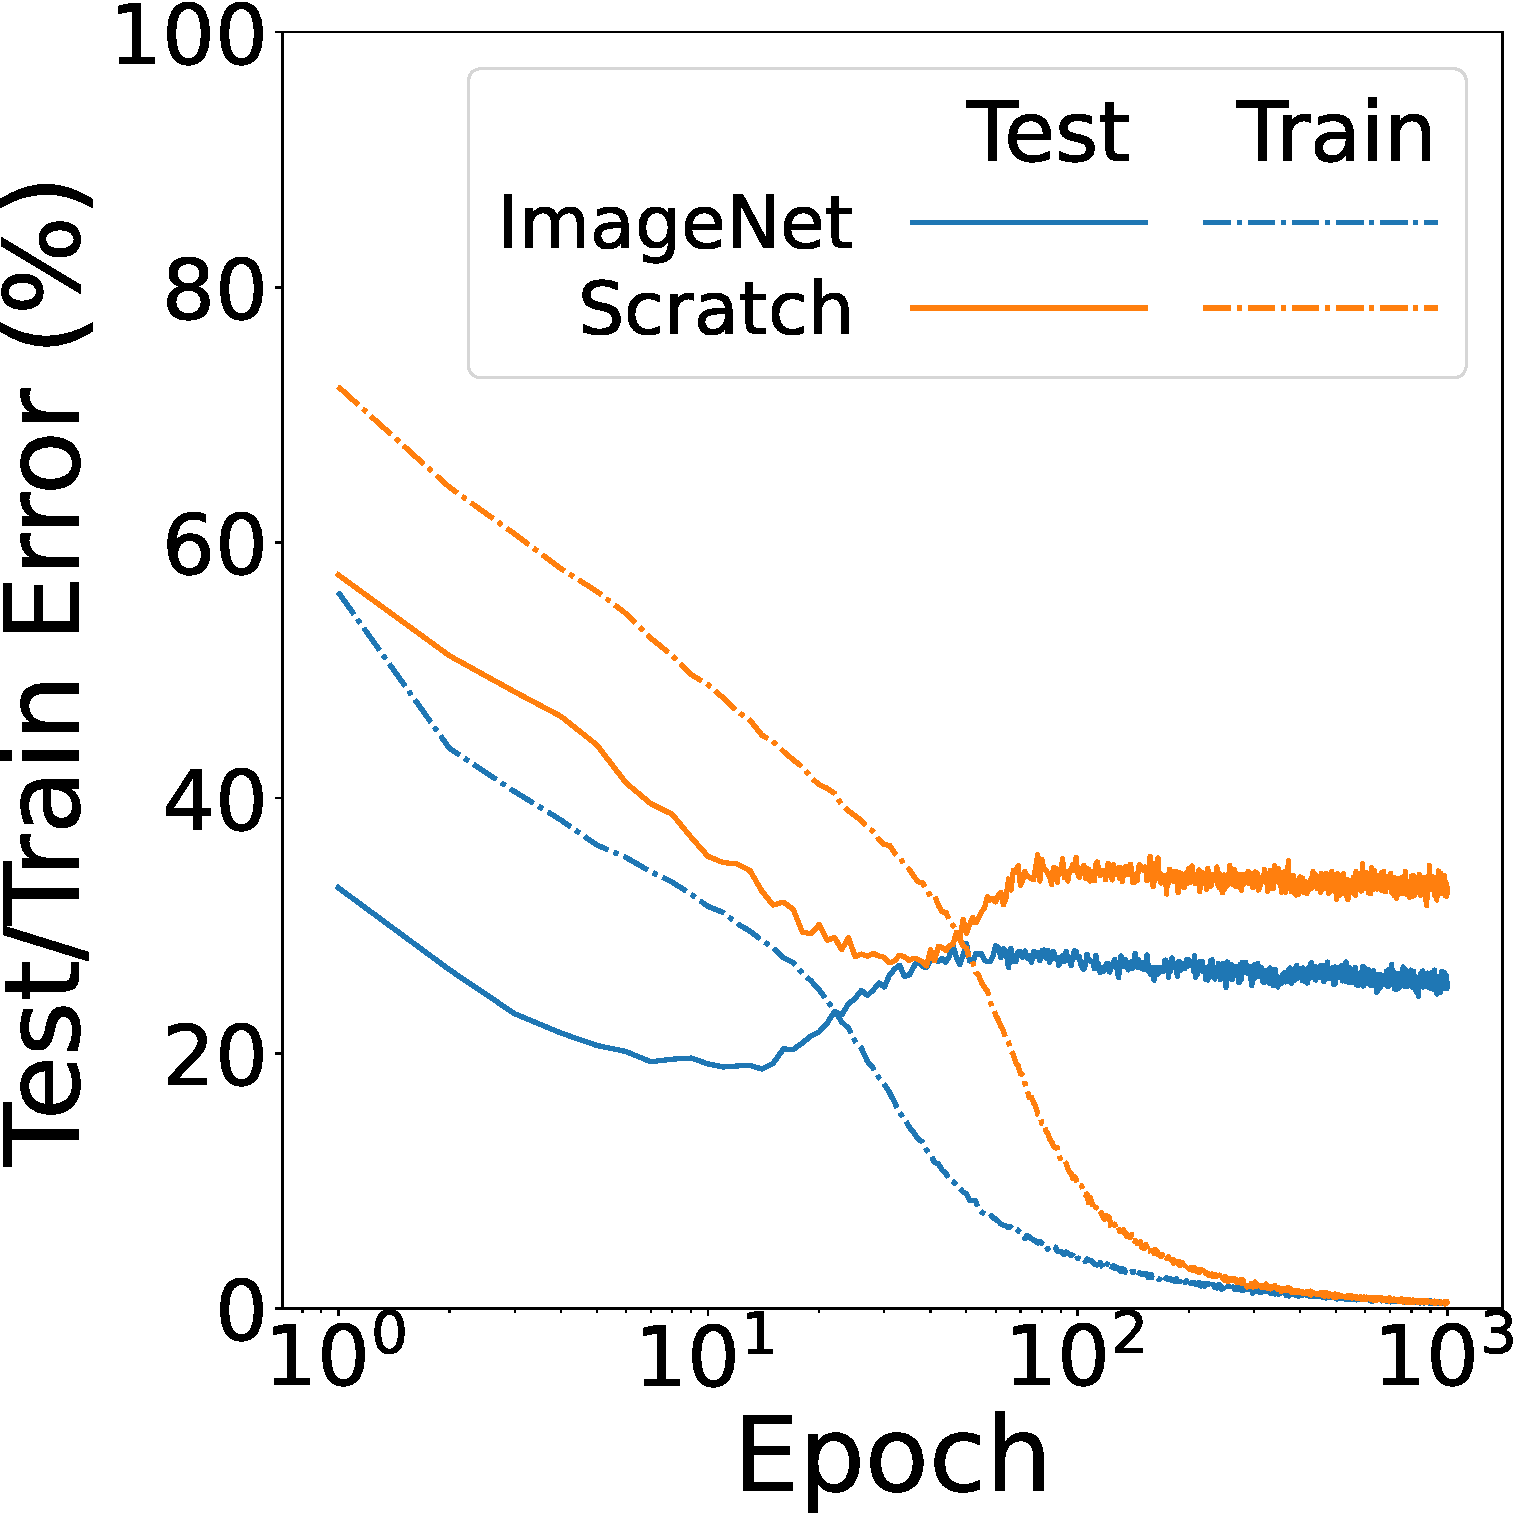
\includegraphics[keepaspectratio, width=0.45\linewidth]{fig/INSR_learning_curv.pdf} &
      \hspace{5pt}
      %---- 2番目の図 --------------------------
      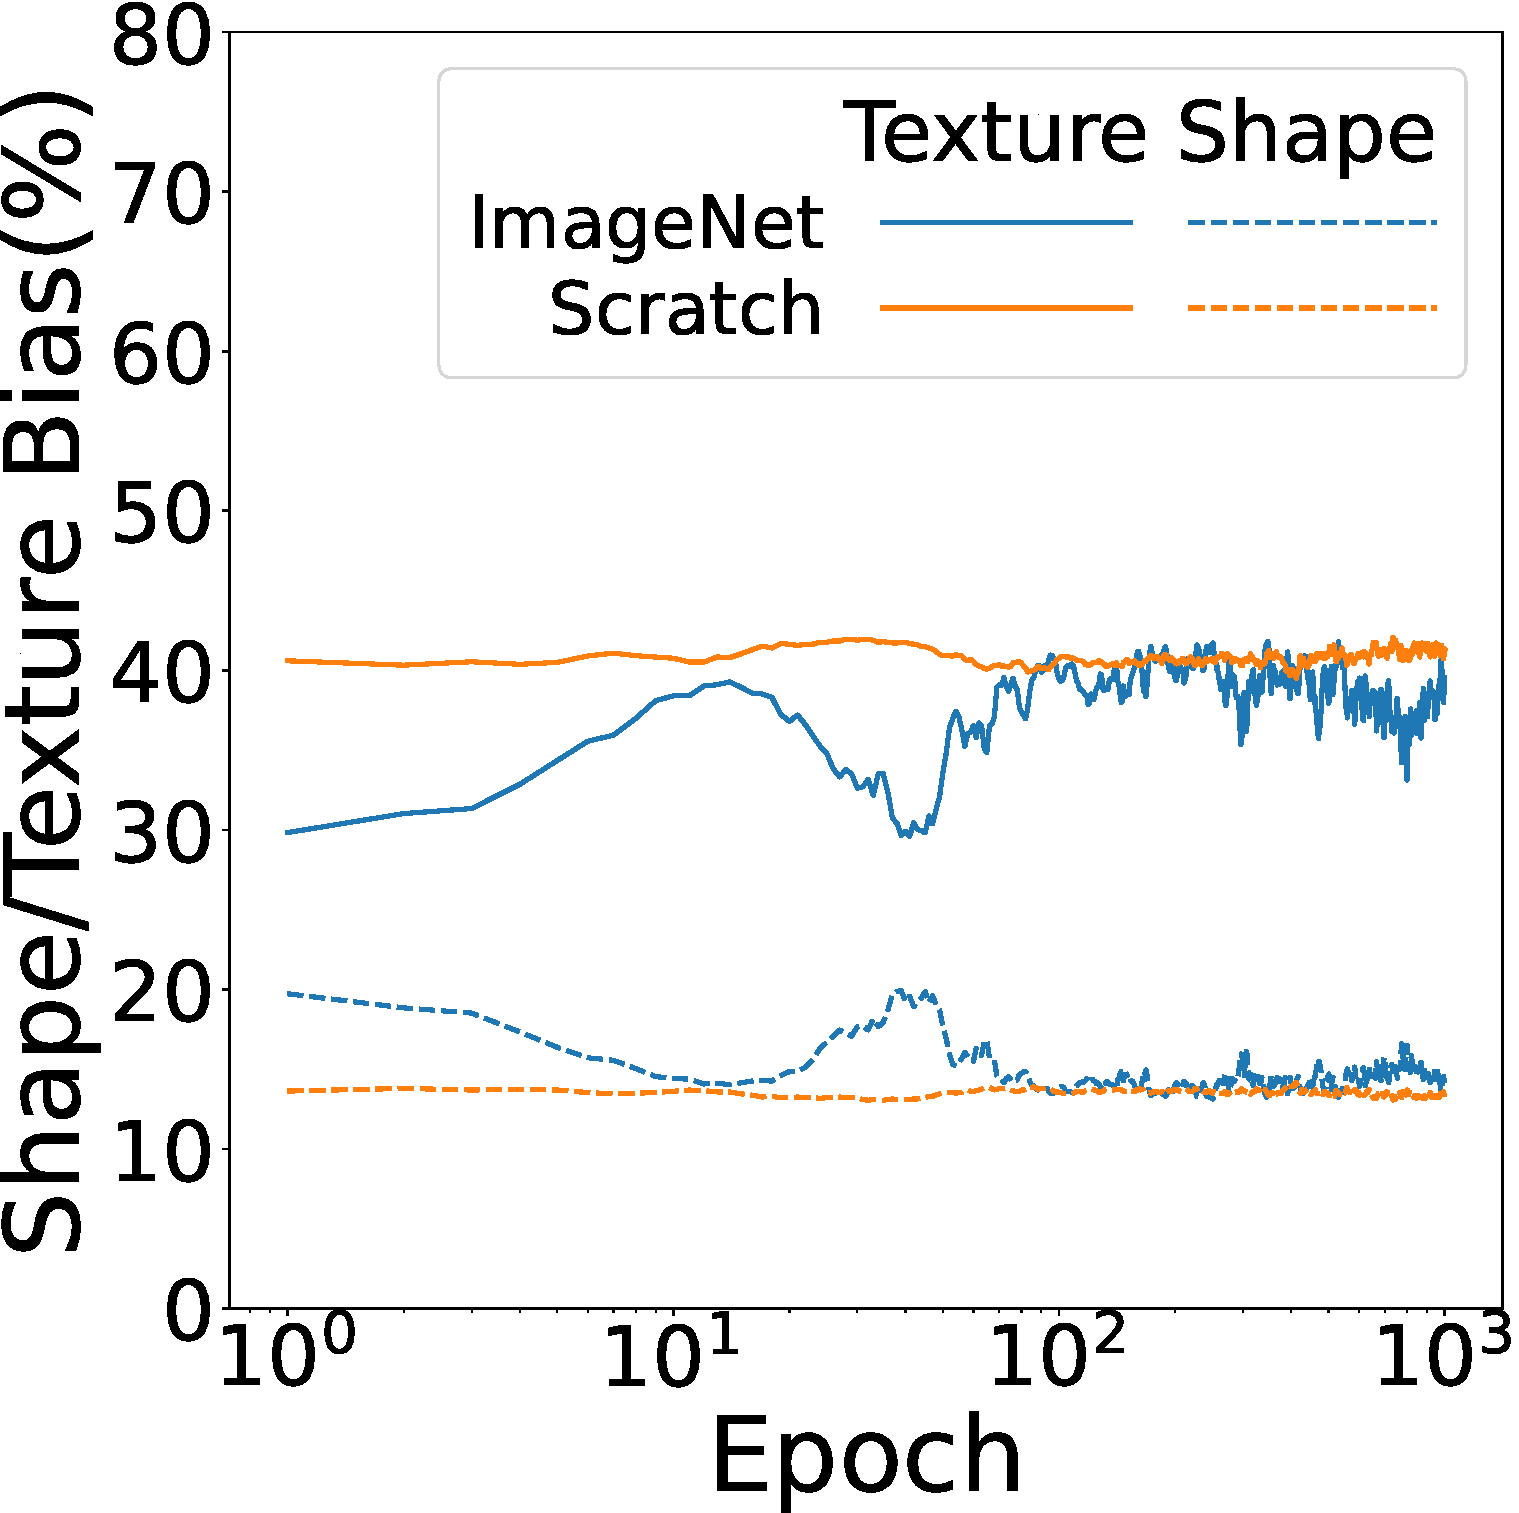
\includegraphics[keepaspectratio, width=0.45\linewidth]{fig/INSR_sha_tex.pdf}
   \end{tabular}
\caption[Learning process with and without pretraining by ImageNet.]{Learning process with and without pretraining by ImageNet. Left: train/test errors Right: shape/texture bias values.}
%Learning curve graphs for double descent and shape/texture bias with and without pretraining on ImageNet. \textbf{Left}:learning curve. \textbf{Right}:model's bias shift.}
\label{fig:comp_INSR}
\end{figure}

\newpage

\subsection[Dataset]{Dataset (\cref{fig:comp_IN_dataset} and \cref{tab:corr_FTdataset})}
データセットを変更した場合の影響を調査するために,CIFAR-10と性質が類似しているCIFAR-100で学習し,CIFAR-10の場合と差異を検証した.結果を\cref{fig:comp_IN_dataset}に,定量評価を\cref{tab:corr_FTdataset}に示す.その結果,CIFAR-10では,Phase1とPhase2において,形状の偏りとの相関は0.778であり,テクスチャの偏りとの相関は-0.778であった.一方,CIFAR-100では,形状の偏りとの相関は-0.689,テクスチャの偏りとの相関は0.745となり,逆相関の関係を示した.CIFAR-10,100ともに,Phase3における形状とテクスチャの相関は,スコア結果からほぼ無視できる.CIFAR-100で観測された逆の相関は,クラス数,クラスの種類,1クラスあたりの枚数などの要因に影響されたCIFAR-10,CIFAR-100特有の特性の差異によるものであると推測される.一方で,逆相関をみせることから,二重降下と偏重度の推移に相関を引き起こす,共通の特性が存在する可能性を示唆している.

また,CIFAR-100から10クラスを抜き出して同様の実験を行った場合にも,CIFAR-100の場合と類似した形状・テクスチャ偏重度の推移を示した.これによってクラス数の差異が直接関係しているわけではないと考えられる.CIFAR-100は20の上位クラスとそれぞれに含まれる5つの下位クラスで構成されている.そのため,たとえば,魚の上位クラスあり,その上位クラスには魚の質感をした5つのクラスが含まれていることになる.それによってCIFAR-10とは重視される特徴に差異が出ている可能性が考えられる.
% データセットを変更した場合の影響を調査するために,CIFAR-10と性質が類似しているCIFAR-100で学習し,CIFAR-10の場合と差異を検証した.結果を\cref{fig:comp_IN_dataset}に,定量評価を\cref{tab:corr_FTdataset}に示す.その結果,CIFAR-10では,Phase1とPhase2において,形状の偏りとの相関は0.778であり,テクスチャの偏りとの相関は-0.778であった.一方,CIFAR-100では,形状の偏りとの相関は-0.689,テクスチャの偏りとの相関は0.745となり,逆相関の関係を示した.CIFAR-10,100ともに,Phase3における形状とテクスチャの相関は,スコア結果からほぼ無視できる.CIFAR-100で観測された逆の相関は,クラス数,クラスの種類,1クラスあたりの枚数などの要因に影響されたCIFAR-10,CIFAR-100特有の特性の差異によるものであると推測される.一方で,逆相関をみせることから,二重降下と偏重度の推移に相関を引き起こす,共通の特性が存在する可能性を示唆している.

\begin{figure}[htb]
\centering
%    \begin{tabular}{c}
%     %---- 最初の図 ---------------------------
%      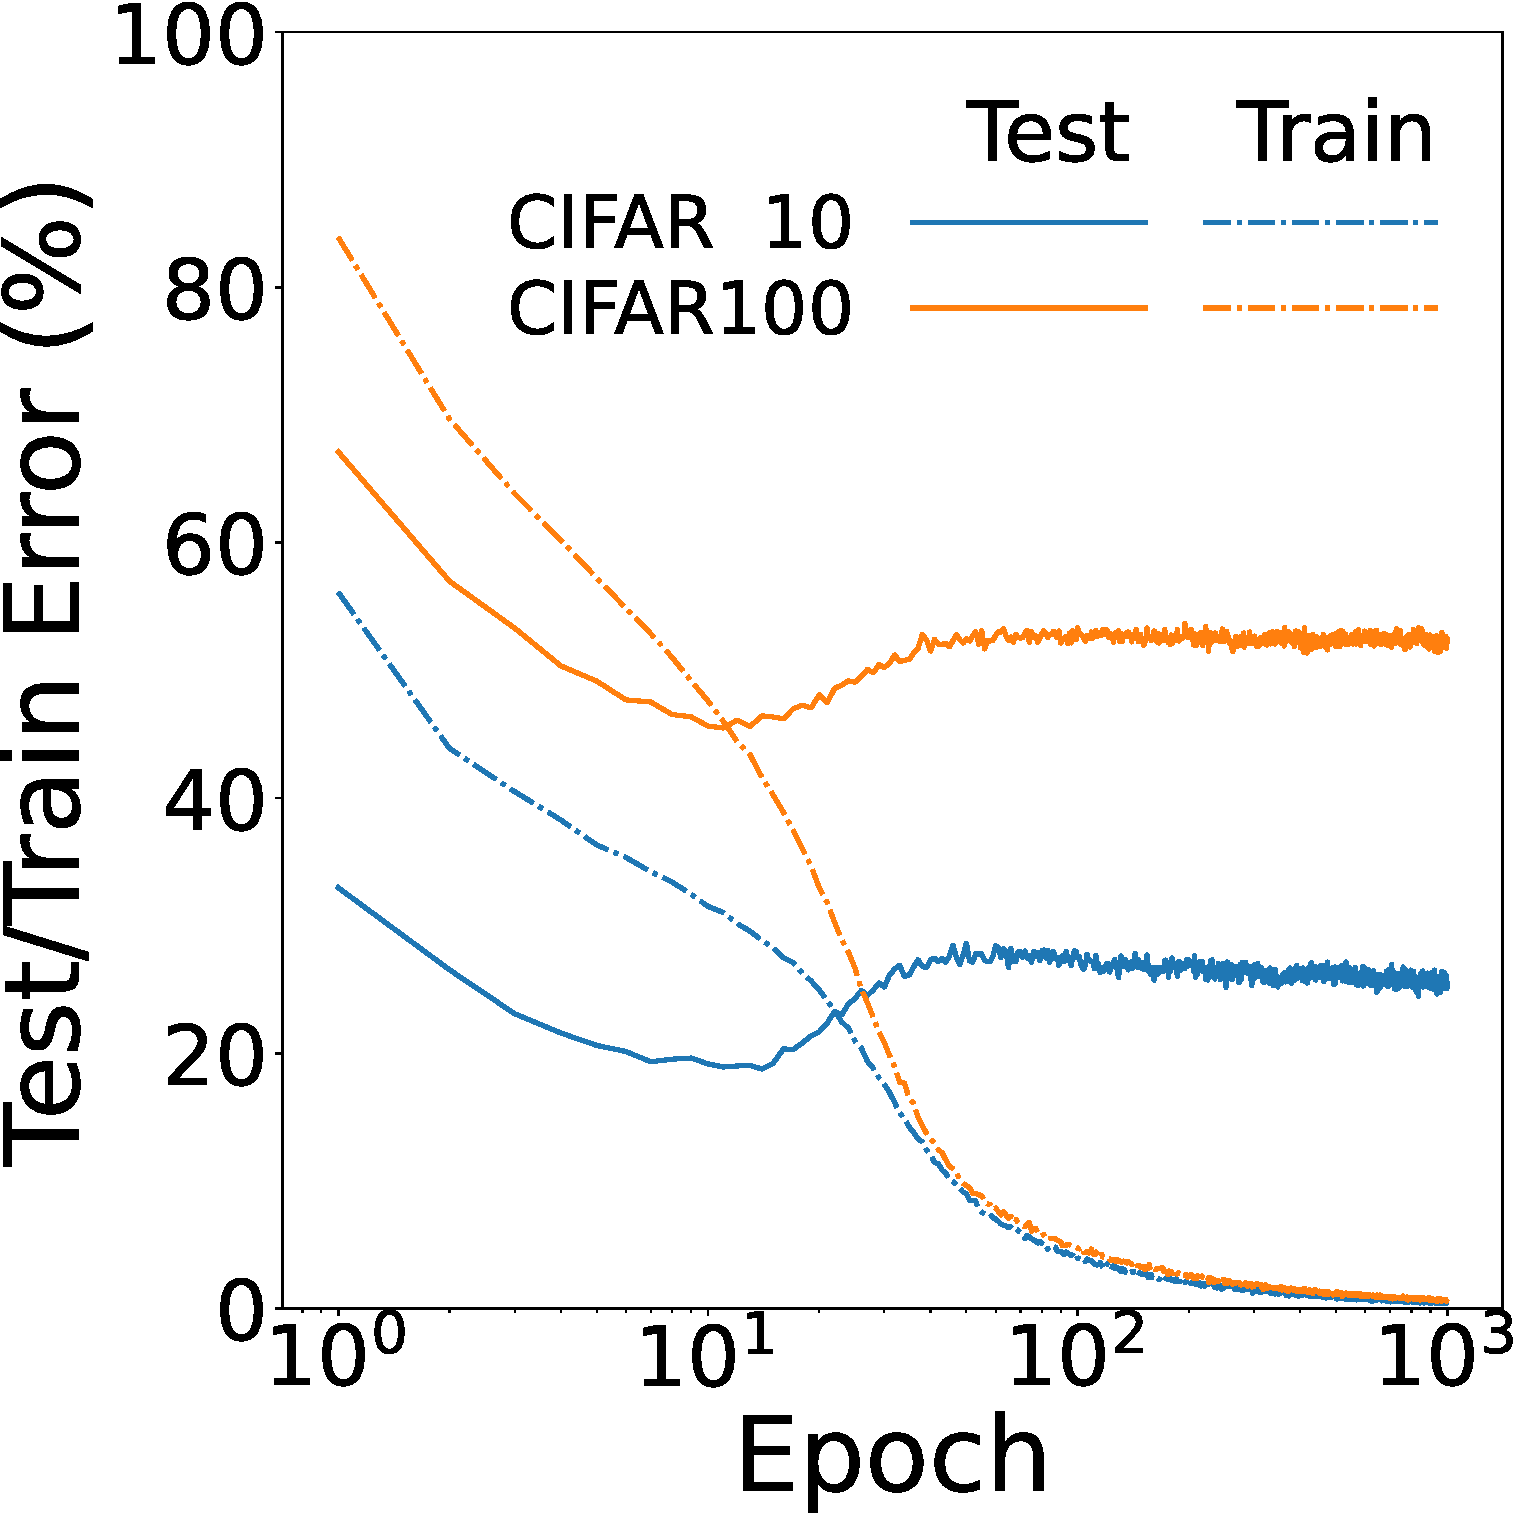
\includegraphics[keepaspectratio, width=0.458\linewidth]{fig/IN_dataset_learning_curv.pdf}
%      %---- 2番目の図 --------------------------
%      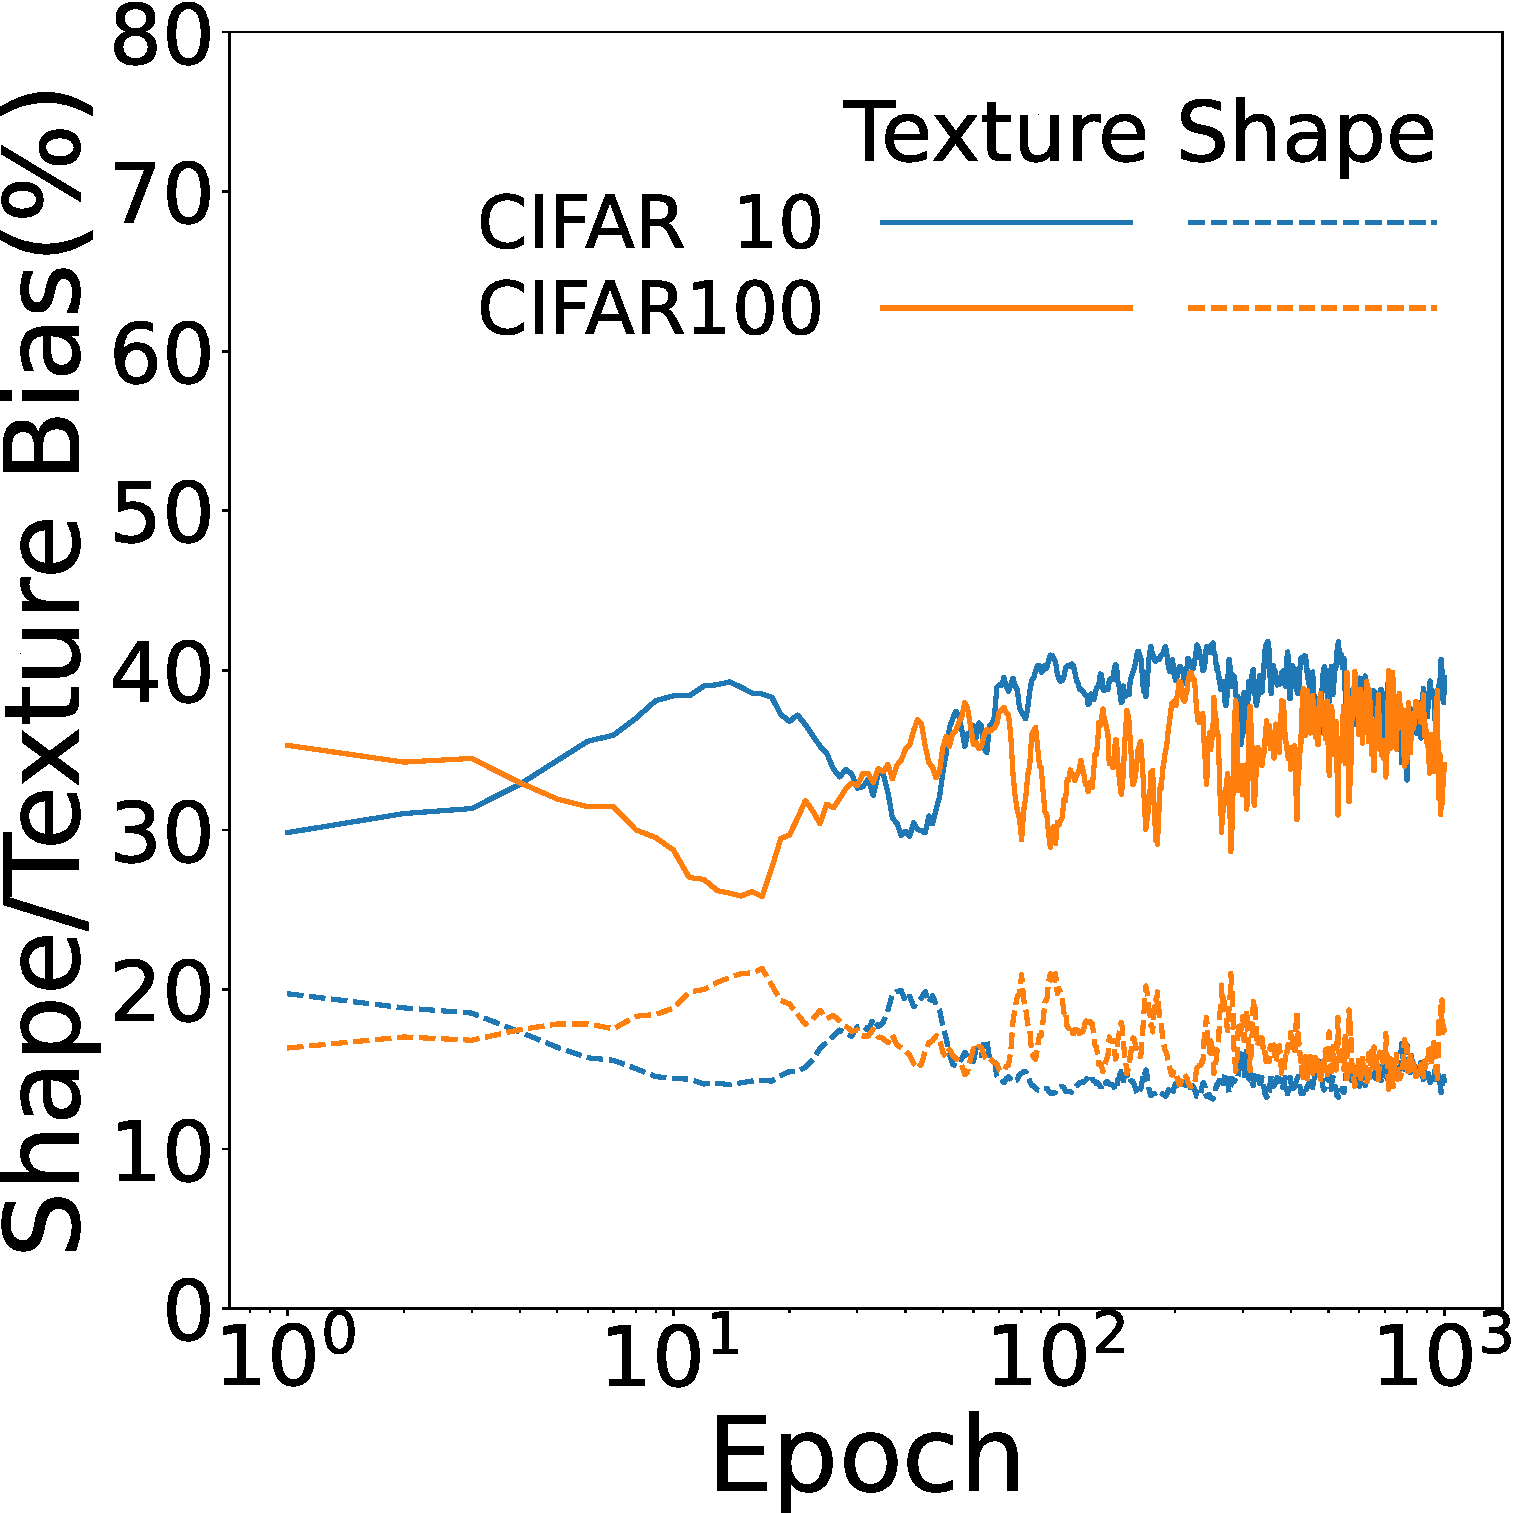
\includegraphics[keepaspectratio, width=0.458\linewidth]{fig/IN_dataset_sha_tex.pdf}
%    \end{tabular}
    \begin{tabular}{cc}
      %---- 最初の図 ---------------------------
      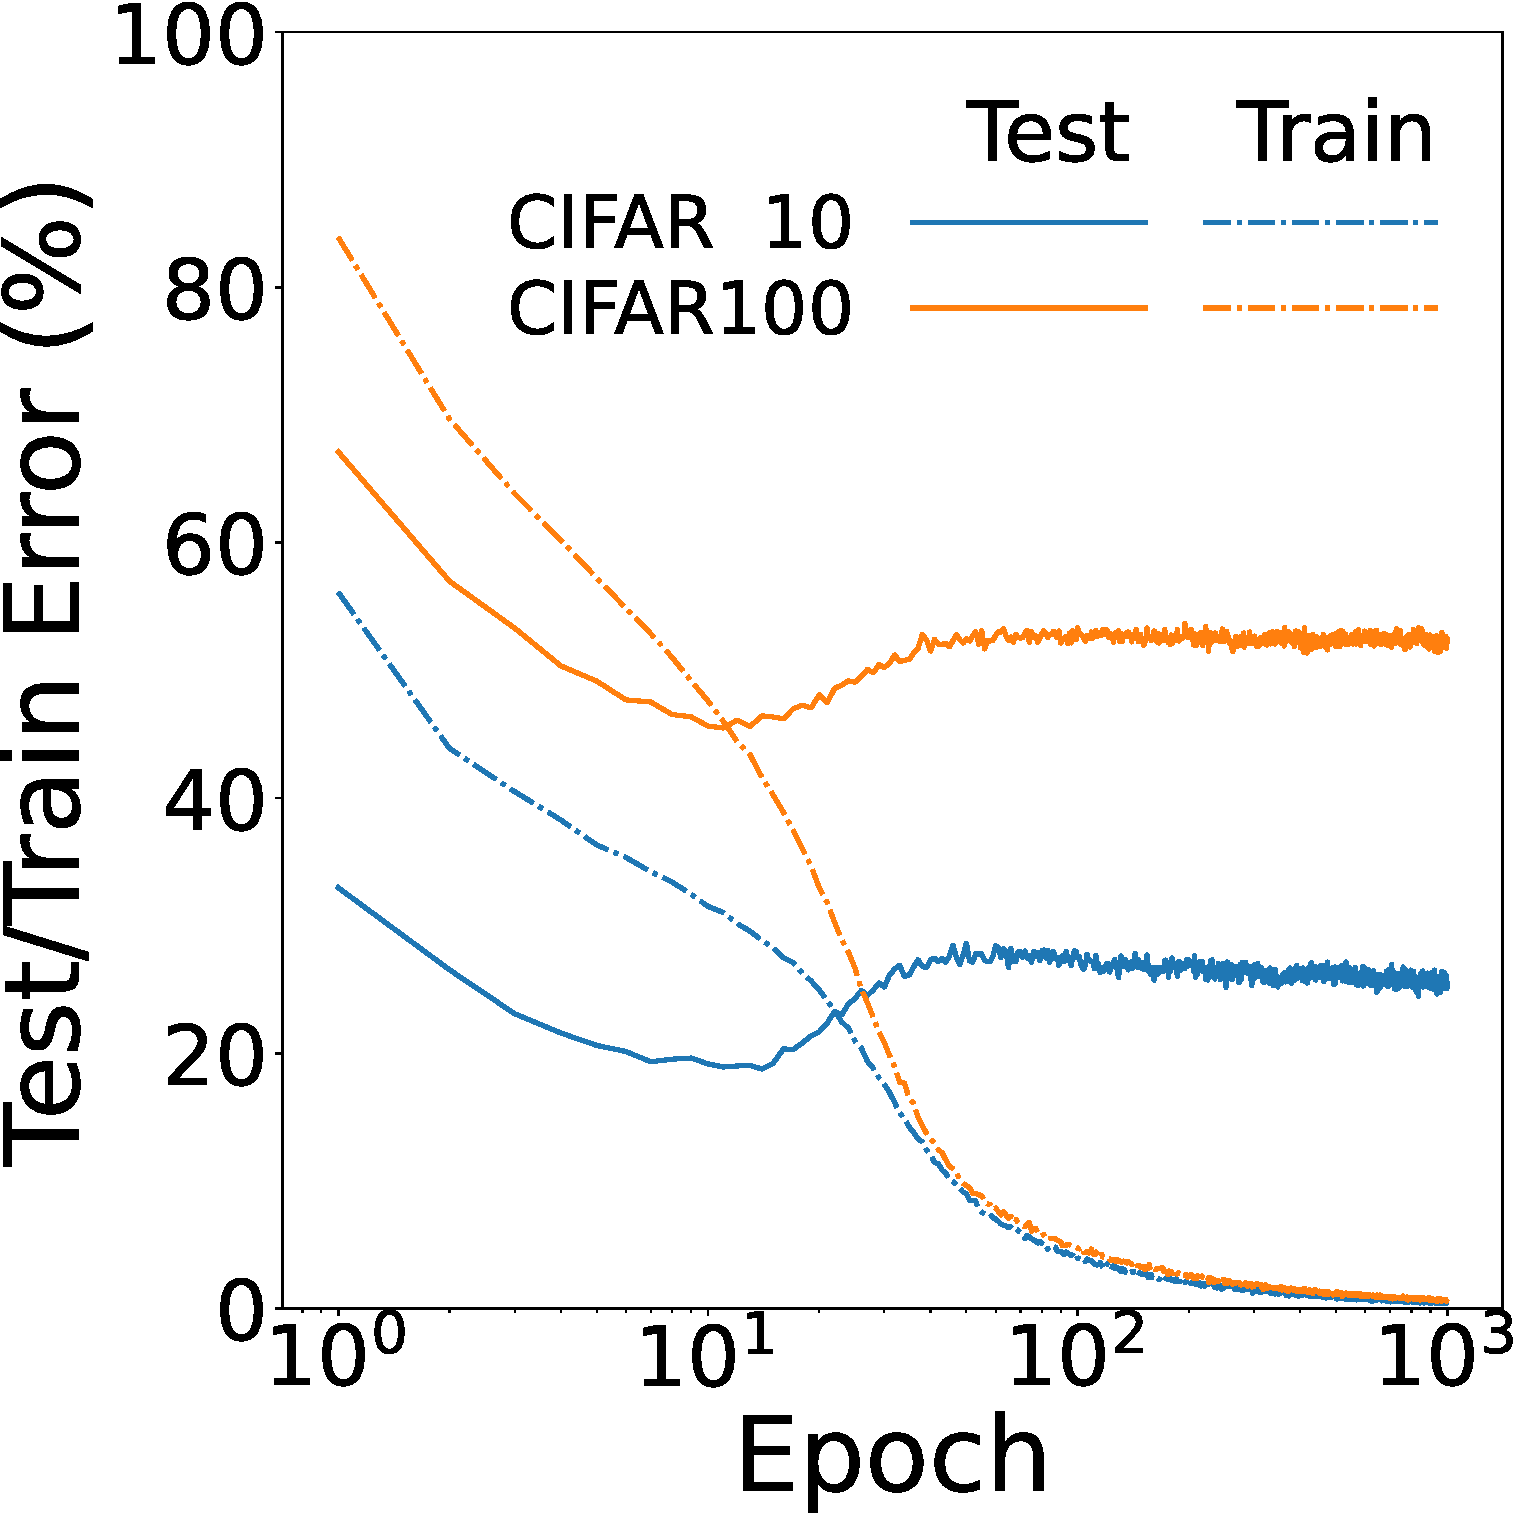
\includegraphics[keepaspectratio, width=0.45\linewidth]{fig/IN_dataset_learning_curv.pdf} &
      \hspace{5pt}
      %---- 2番目の図 --------------------------
      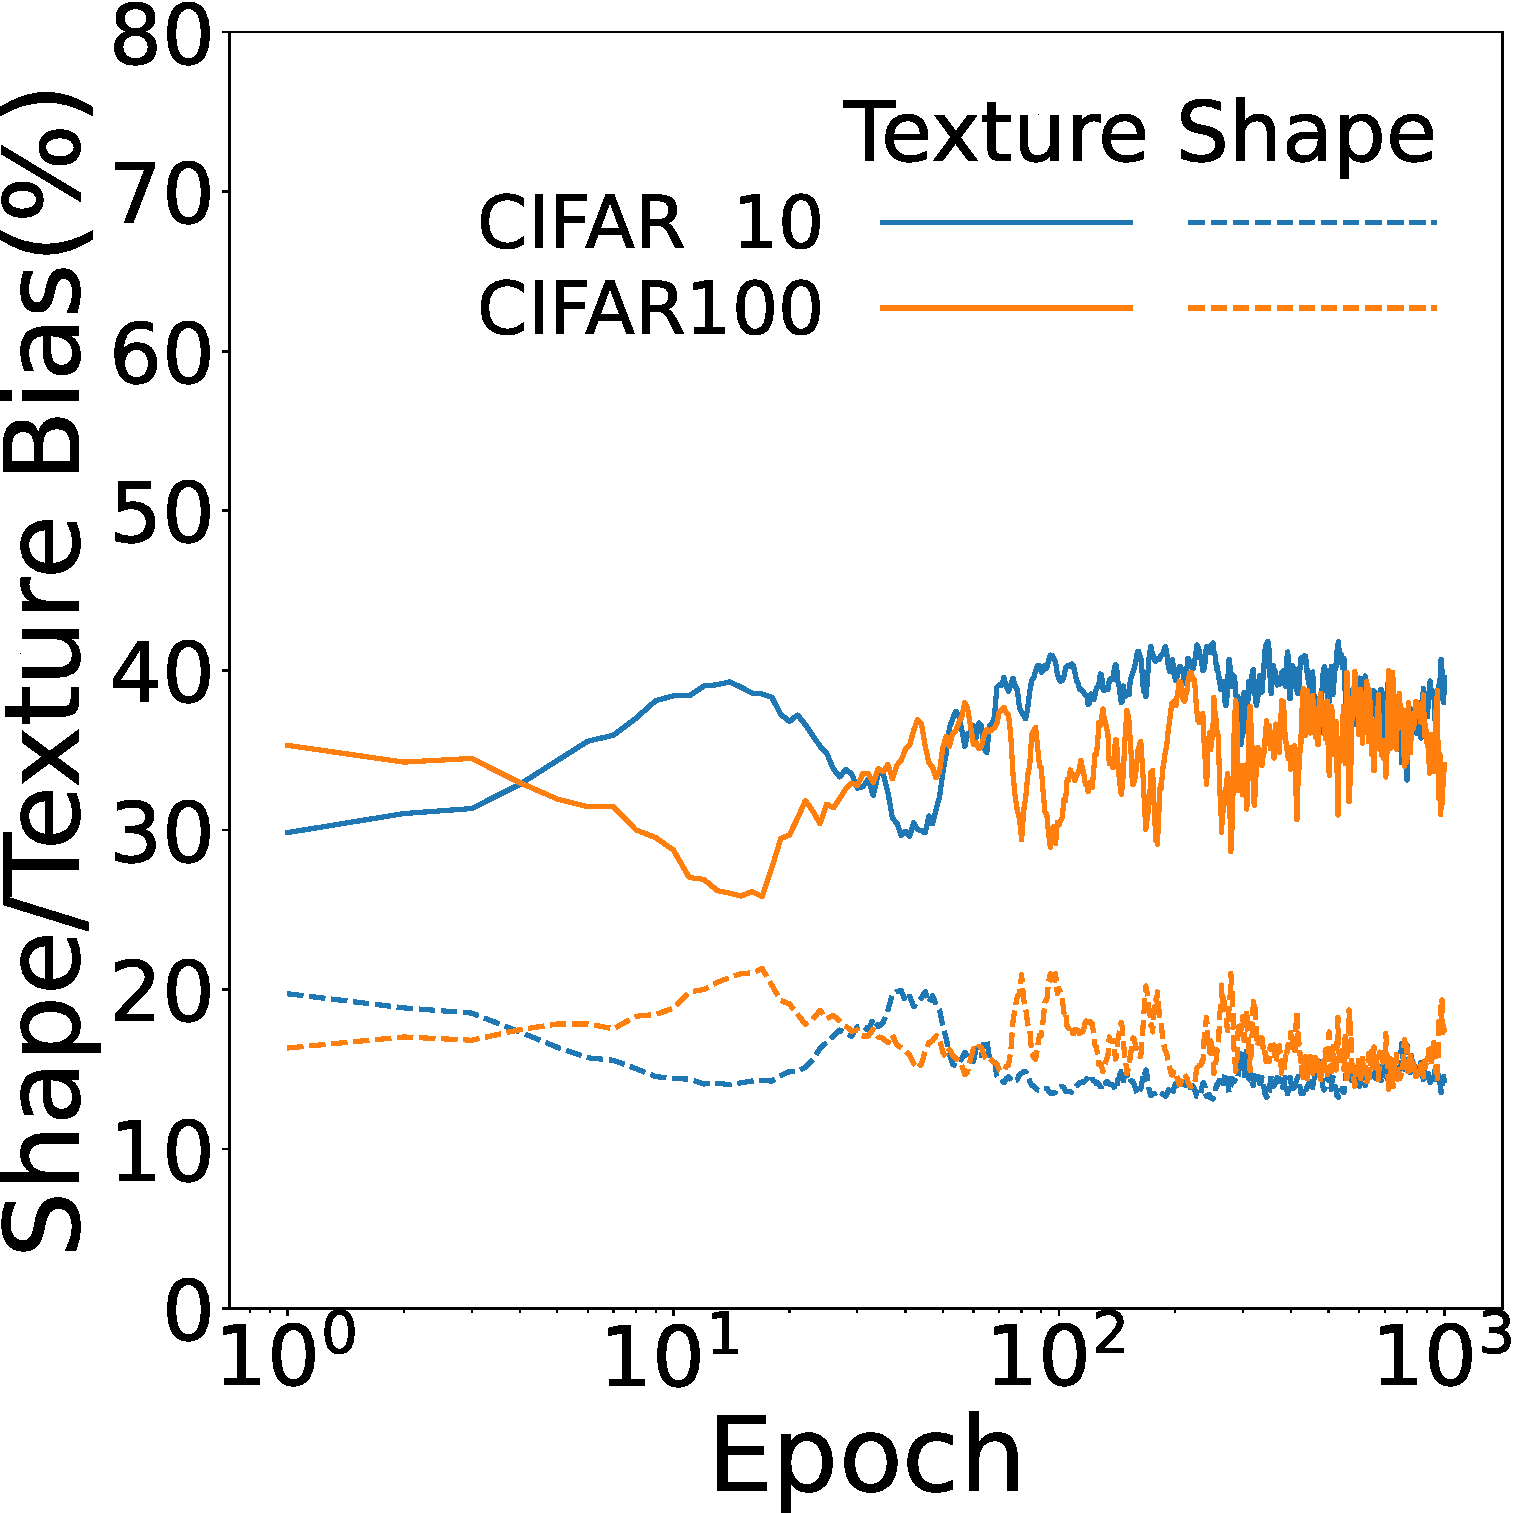
\includegraphics[keepaspectratio, width=0.45\linewidth]{fig/IN_dataset_sha_tex.pdf}
    \end{tabular}
\caption[Learning process by different tasks, CIFAR-10 and CIFAR-100.]{Learning process by different tasks, CIFAR-10 and CIFAR-100. Left: train/test errors Right: shape/texture bias values.
%Learning curve graphs for double descent and shape/texture bias for different datasets. \textbf{Left}:learning curve. \textbf{Right}:model's bias shift.
% Epoch-wise double descent vs model's shape/texture bias shift in fine-tuning dataset differences. \textbf{Left}:learning curve. \textbf{Right}:model's bias shift.
}
\label{fig:comp_IN_dataset}
\end{figure}

\begin{table}[htb]
    \centering
    \caption{
    % sample
    % 各ステージ毎の相関係数.相関係数を計算するために利用したデータの区間およびTest Errorと形状偏重度で計算した相関係数(Shape corr),TestErrorとテクスチャ偏重度で計算した相関係数(Texture corr)及び二つの相関係数から計算した最終的なスコアを示している.
    % 各データセットでfine-tuningした場合におけるPhase1, 2,およびPhase3での相関係数とscore.Test errorとShape biasとの相関係数(SB),Test errorとTexture biasとの相関係数(TB)及び二つの相関係数から計算したscoreを示している.
    Correlation coefficients and scores in Phase 1, 2 and Phase 3 for different datasets.
    }
    %old version
    % \begin{tabular}{c|c|c} 
    % \toprule[0.8pt]
    % Datasets  &  Correlation area &  score\\
    %  \midrule[0.5pt]
    % CIFAR10  & Stage1,2 (2-41) &0.778\\
    % CIFAR100 & Stage1,2 (2-55) &0.717\\
    % \toprule[0.8pt]
    % \end{tabular}
    % \label{tab:corr_FTdataset}
    \scalebox{1.2}{
    \begin{tabular}{c|SSc|SSc} 
    \toprule[0.8pt]
    \multirow{2}{*}{CNN}  &  \multicolumn{3}{c|}{Correlation of Phase1,2} &  \multicolumn{3}{c}{Correlation of Phase3}\\
     \cline{2-7}
             & {SB} & {TB} & Score & {SB} & {TB} & Score \\
     \midrule[0.5pt]
    C10  &0.778&-0.778 & 0.778 & -0.026&0.118 & 0.072\\
    C100 &-0.689&0.745 & 0.717&0.002&0.013 & 0.007\\
    \toprule[0.8pt]
    \end{tabular}
    }
    \label{tab:corr_FTdataset}
\end{table}

\newpage

\subsection[ResNet family]{ResNet family (see \cref{fig:comp_model} and \cref{tab:corr_model})}
モデルのパラメータ数の影響,特にResNet family内で一般性があるのかを検証するため,ResNet18と同様の論文で提案されているResNet34,ResNet50でも実験を行った.使用するモデルをResNet34,ResNet50に変更した場合の結果を\cref{fig:comp_model}に,定量的な評価のための表を\cref{tab:corr_model}に示す.ResNet34においては,偏重度の推移に相関があるように見られ,Phase1,2のScoreが0.517とResNet18の場合と同様の相関を定量的にも示す.しかし,ResNet50においては,偏重度の推移には定性的にはPhase2での変化が見られず,定量的にも相関がみられない.この結果の理由として,ResNetは,ResNet18,ResNet34,ResNet50とパラメータ数が増加するため,パラメータ数の上昇に従って,相関が消える可能性が考えられる.また,使用したResNetの構造の差異を考えると,ResNet18,ResNet34はbasic blockと呼ばれる構造から形成されているのに対して,ResNet50はbottleneckと呼ばれる構造から形成されており,この点が影響を与えた可能性も考えられる.

\begin{figure}[htb]
\centering
   \begin{tabular}{cc}
      %---- 最初の図 ---------------------------
      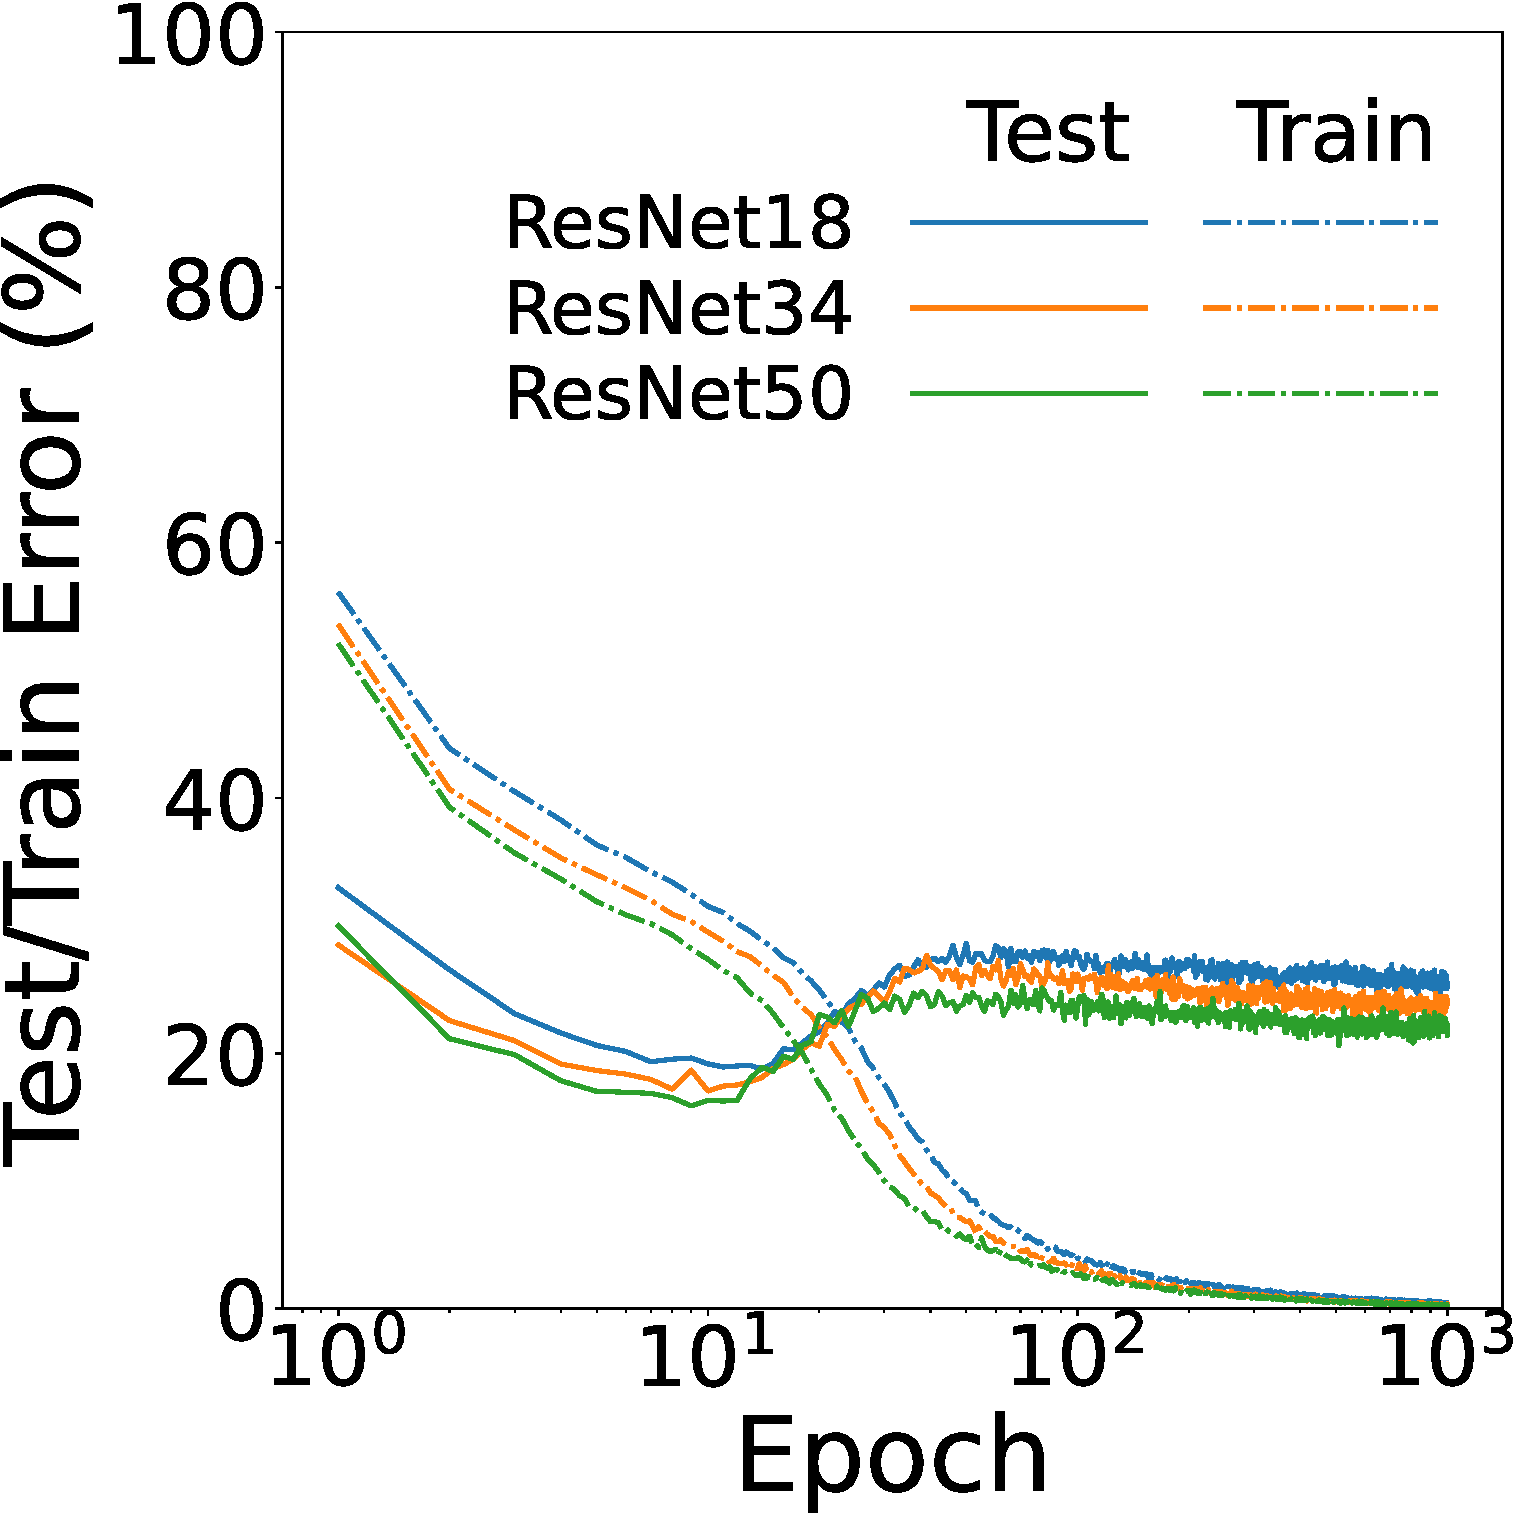
\includegraphics[keepaspectratio, width=0.45\linewidth]{fig/model_learning_curv.pdf} &
       \hspace{5pt} 
      %---- 2番目の図 --------------------------
      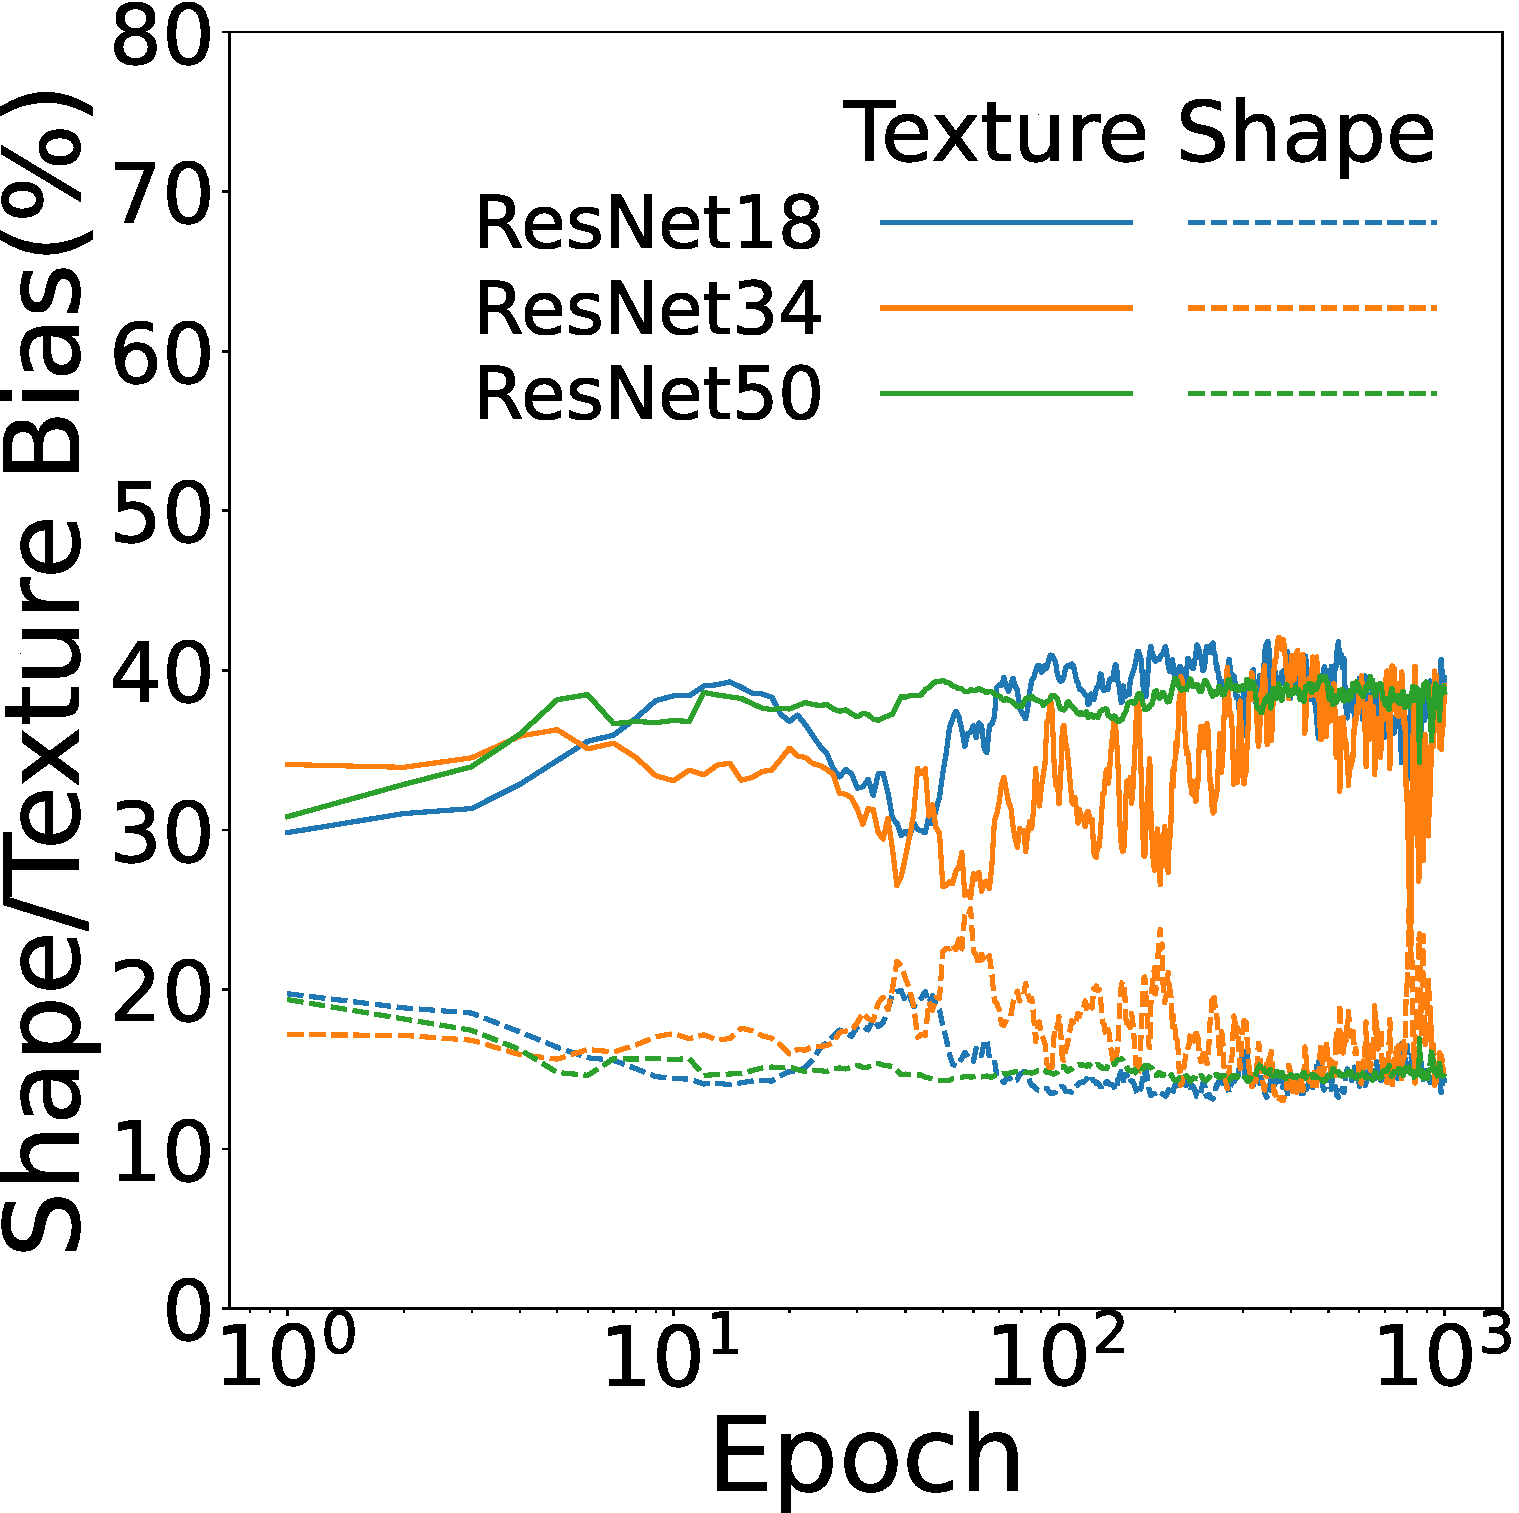
\includegraphics[keepaspectratio, width=0.45\linewidth]{fig/model_sha_tex.pdf}
   \end{tabular}
\caption[Learning process under various size conditions of ResNet family.]{
Learning process under various size conditions of ResNet family. Left: train/test errors Right: shape/texture bias values.}
% Learning curve graphs for double descent and shape/texture bias for different models. \textbf{Left}:learning curve. \textbf{Right}:model's bias shift.}
\label{fig:comp_model}
\end{figure}

\begin{table}[htb]
    \centering
    \caption{
    % sample
    % 各ステージ毎の相関係数.相関係数を計算するために利用したデータの区間およびTest Errorと形状偏重度で計算した相関係数(Shape corr),TestErrorとテクスチャ偏重度で計算した相関係数(Texture corr)及び二つの相関係数から計算した最終的なスコアを示している.
    % 各モデルを使用した場合におけるPhase1, 2,およびPhase3での相関係数とscore.Test errorとShape biasとの相関係数(SB),Test errorとTexture biasとの相関係数(TB)及び二つの相関係数から計算したscoreを示している.
    Correlation coefficients and scores in Phase 1, 2 and Phase 3 for different ResNet Family.
    }
    % \begin{tabular}{c|c|c} 
    % \toprule[0.8pt]
    % Model  & Correlation area&  score\\
    %  \midrule[0.5pt]
    % ResNet18  & Stage1,2 (2-41) &0.778\\
    % ResNet34 & Stage1,2 (2-41) &0.517\\
    % ResNet50 & Stage1,2 (2-180) &0.215\\
    % \toprule[0.8pt]
    % \end{tabular}
    \scalebox{1.2}{
    \begin{tabular}{c|SSc|SSc} 
    \toprule[0.8pt]
    \multirow{2}{*}{CNN}  &  \multicolumn{3}{c|}{Correlation of Phase1,2} &  \multicolumn{3}{c}{Correlation of Phase3}\\
     \cline{2-7}
             & {SB} & {TB} & Score & {SB} & {TB} & Score \\
     \midrule[0.5pt]
    ResNet18 &0.778&-0.778 & 0.778 & -0.026&0.118 & 0.072\\
    ResNet34 &0.498& -0.536 & 0.517 & 0.165 & -0.281 & 0.223\\
    ResNet50 &-0.153&0.136& 0.144 & -0.097&0.064 & 0.080\\
    \toprule[0.8pt]
    \end{tabular}
    }
    \label{tab:corr_model}
\end{table}

\newpage

\subsection[CNN models]{CNN models (see \cref{fig:comp_cnn_model} and \cref{tab:corr_CNN_model})}
ResNetとは異なるCNNモデルを使用した場合における,二重降下と形状・テクスチャ偏重度の推移への影響を検証した.具体的には,DenseNet121\footnote{https://pytorch.org/vision/0.9/\_modules/torchvision/models/densenet.html\#densenet121}~\cite{DenseNet},MobileNetV2\footnote{https://pytorch.org/vision/0.9/models.html?highlight=mobilenet\#torchvision.models.mobilenet\_v2}~\cite{mobileNetV2},EffecientNet B0\footnote{https://pytorch.org/vision/0.14/models/generated/torchvision.models.efficientnet\_b0.html?\\highlight=efficientnet\#torchvision.models.efficientnet\_b0}~\cite{EffectiveNet}を使用した. ResNetが4つのブロックと,1ブロックごとに接続されるskip connectionから構成されるのに対して,DenseNetは4つのblockと各blockから異なるすべてのblockに接続されるskip connectionから構成されるCNN,MoblieNetV2はモバイル向けに効率アが図られたCNN,EfficientNetはNeural Architecture Searchと呼ばれる手法により,最適化が図られたCNNである.異なるCNNを使用した場合の結果を\cref{fig:comp_cnn_model}に,定量的な評価のための表を\cref{tab:corr_CNN_model}に示す.DenceNet121,MobileNetV2を使用した場合において,緩やかであるが,推移が相関しているように観察でき,Scoreも0.324,0.509と,定量的にも相関がみられた.反対に,EfficientNet B0においては特に相関は見られなかった.この点に関して,DenseNet121,MobileNetV2,およびEfficientNet B0の間に何らかの差異が存在すると考えられるが,これらのモデルの構造的な明確な差異は見受けられないため,原因は不明である.また,EfficientNetの場合においては今までのどの条件とも異なる偏重度の推移を見せており,特徴の学習過程という観点において,その他のモデルと大きく異なる可能性が示唆される.

\begin{figure}[htb]
\centering
   \begin{tabular}{cc}
      %---- 最初の図 ---------------------------
      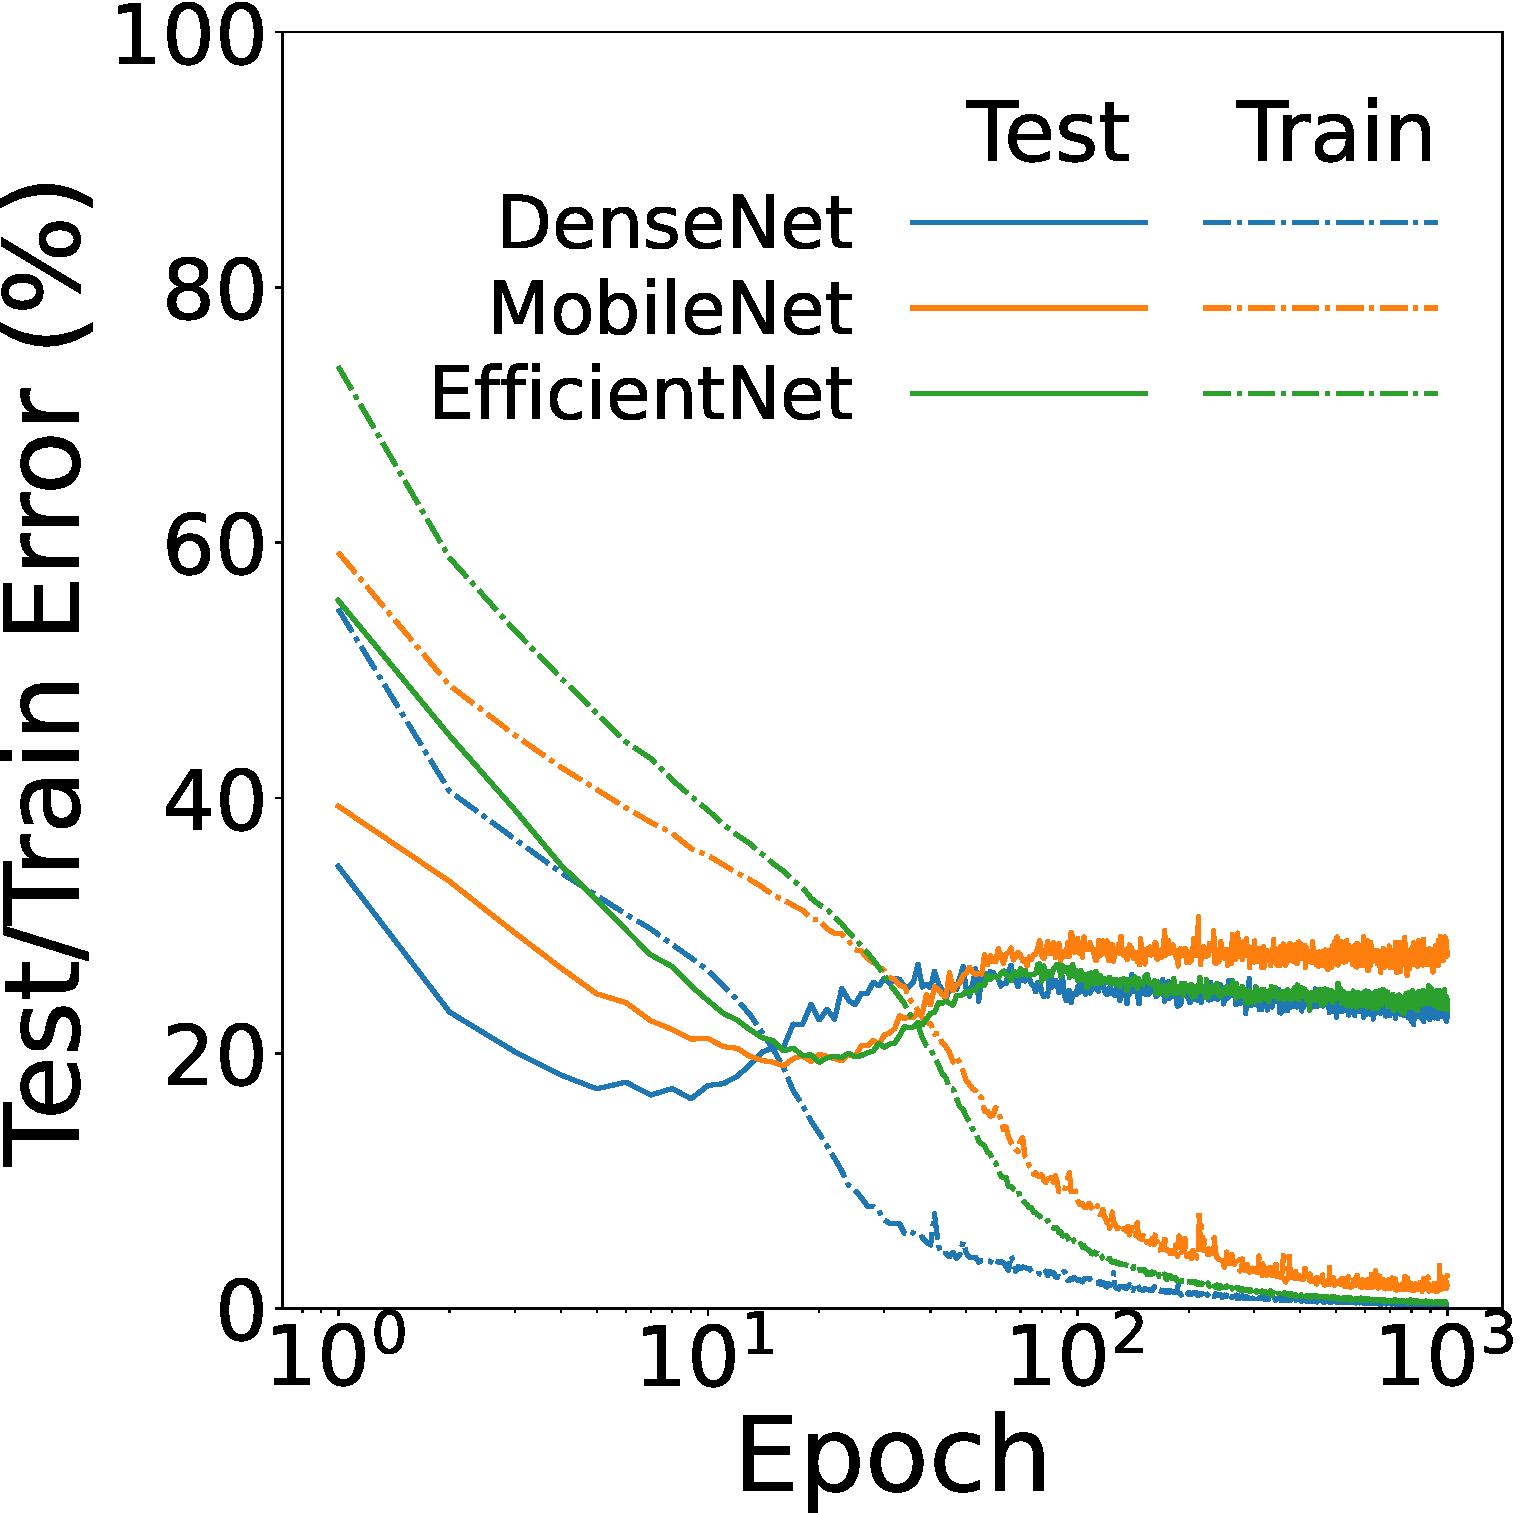
\includegraphics[keepaspectratio, width=0.45\linewidth]{fig/cnn_model_learning_curv.pdf} &
       \hspace{5pt} 
      %---- 2番目の図 --------------------------
      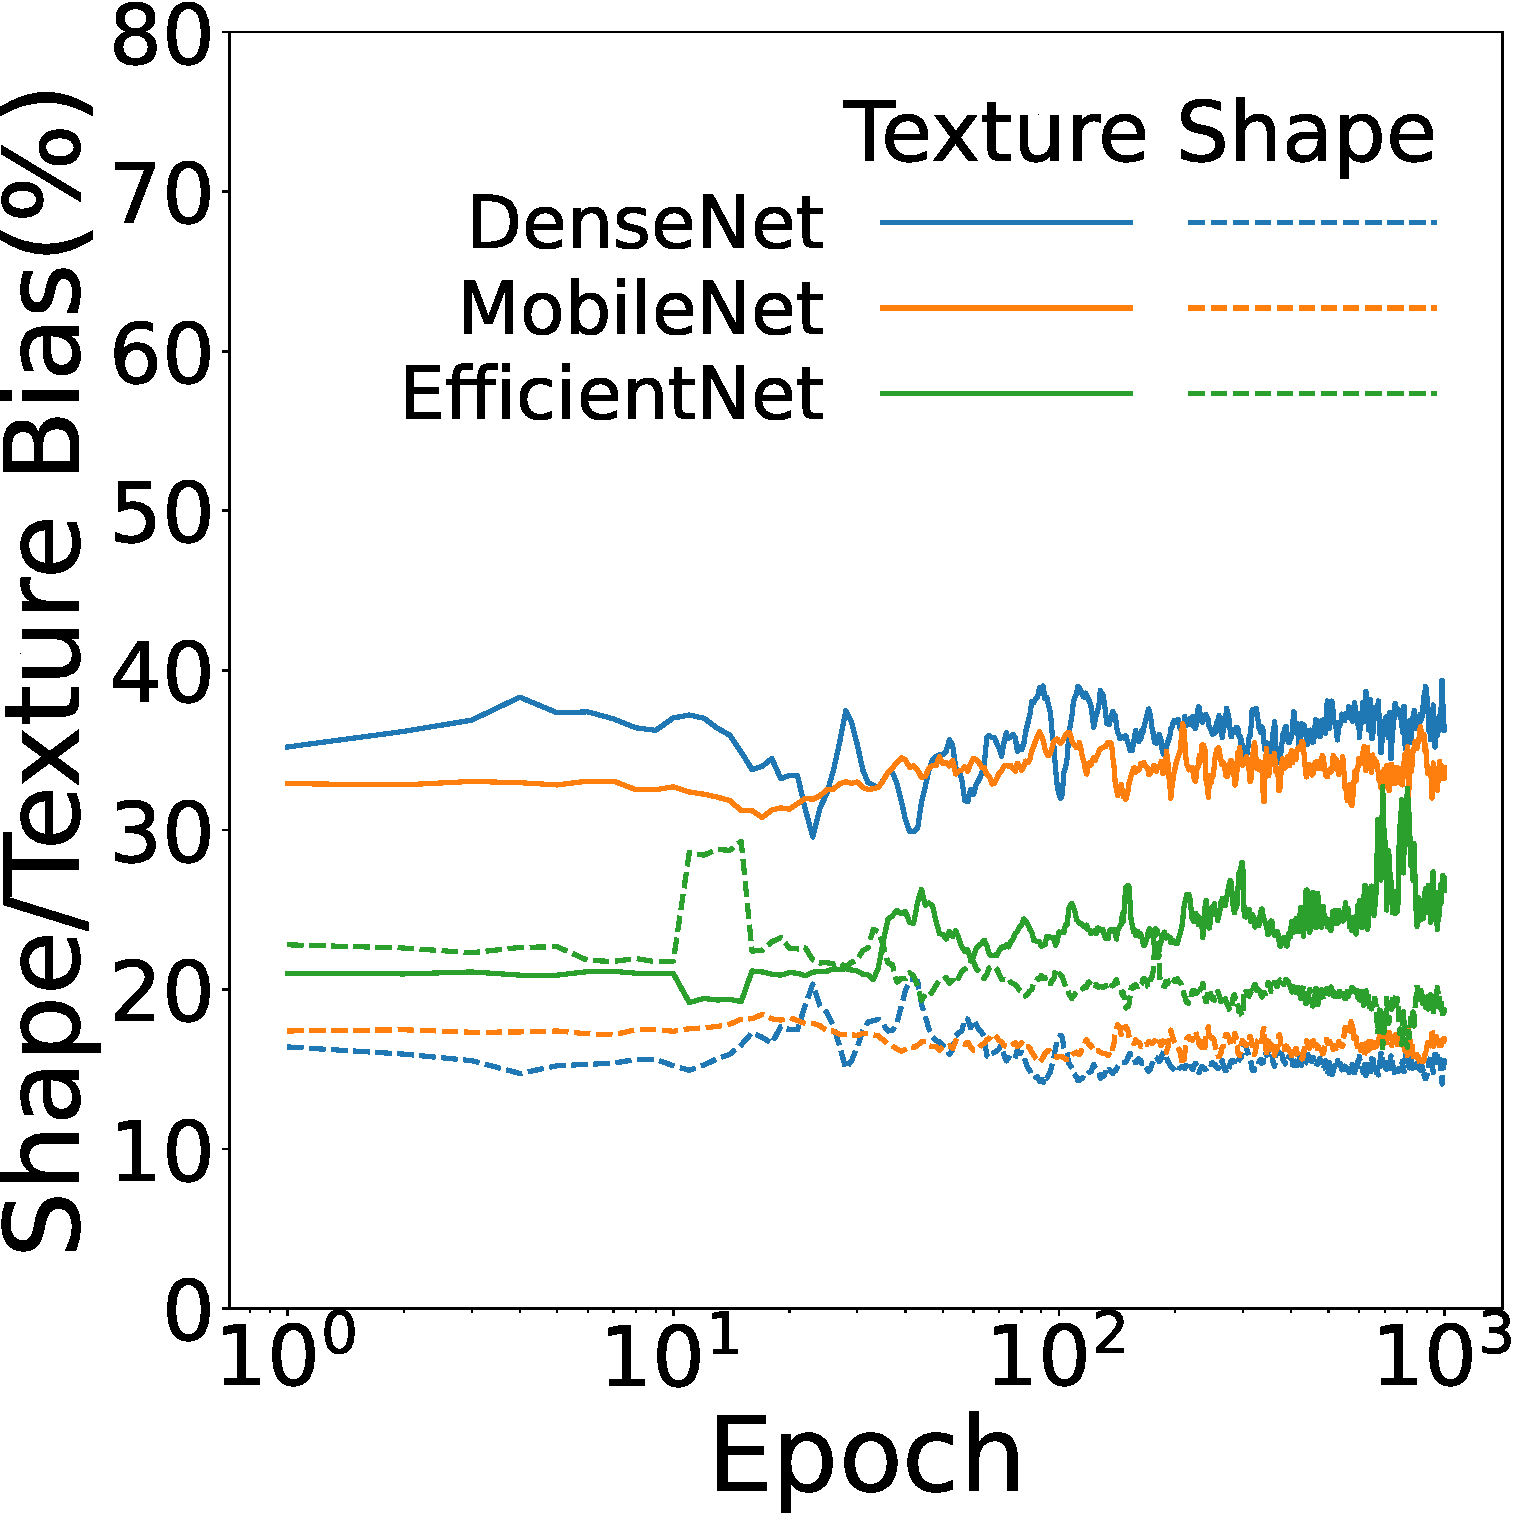
\includegraphics[keepaspectratio, width=0.45\linewidth]{fig/cnn_model_sha_tex.pdf}
   \end{tabular}
\caption[Learning process under various size conditions of CNN models.]{Learning process under various size conditions of CNN models. Left: train/test errors Right: shape/texture bias values.}
% Learning curve graphs for double descent and shape/texture bias for different models. \textbf{Left}:learning curve. \textbf{Right}:model's bias shift.}
\label{fig:comp_cnn_model}
\end{figure}

\begin{table}[htb]
    \centering
    \caption{
    % sample
    Correlation coefficients and scores in Phase 1, 2 and Phase 3 for different CNN models.
    }
    \scalebox{1.2}{
    \begin{tabular}{c|SSc|SSc} 
    \toprule[0.8pt]
    \multirow{2}{*}{CNN}  &  \multicolumn{3}{c|}{Correlation of Phase1,2} &  \multicolumn{3}{c}{Correlation of Phase3}\\
     \cline{2-7}
             & {SB} & {TB} & Score & {SB} & {TB} & Score \\
     \midrule[0.5pt]
    DenseNet &0.326&-0.322 & 0.324 & 0.293&-0.289 & 0.291\\
    MobileNet &-0.506&0.511 & 0.509&-0.016&0.036 & 0.026\\
    EfficientNet &-0.029&0.000 & 0.014&0.316&-0.343 & 0.330\\
    \toprule[0.8pt]
    \end{tabular}
    }
    \label{tab:corr_CNN_model}
\end{table}

\newpage

\subsection[Batch size]{Batch size (see \cref{fig:comp_batchsize} and \cref{tab:corr_batchsize})}
バッチサイズを変更した場合における,二重降下と形状・テクスチャ偏重度の推移への影響を検証した.異なるバッチサイズを使用した場合の結果を\cref{fig:comp_cnn_model}に,定量的な評価のための表を\cref{tab:corr_CNN_model}に示す.バッチサイズの減少に従って,テスト誤り率の曲線が右上にシフトしている.また,形状・テクスチャ偏重度の推移も,曲線の大きく落ち込んでいるところに注目すると,バッチサイズの減少に従って右にシフトしているよう見受けられる.定性的には,どの条件も相関を示していない.また,バッチサイズ4においては,定義した手法においては,Phaseを分割不可能であったため,データなしとしている.

このような二重降下の挙動の差異について,バッチサイズの低下によってepochあたりのイテレーション数は増加するため,バッチサイズが少ないほど,二重降下の挙動が右にシフトするのは予期しない結果となった.しかし,バッチサイズの増加によって学習の安定性が上昇するため,この影響であると考えられる.加えて,バッチサイズの増加につれて,右にシフトするのかについては,検証の余地がある.

\begin{figure}[htb]
\centering
   \begin{tabular}{cc}
      %---- 最初の図 ---------------------------
      \hspace{-5mm}
      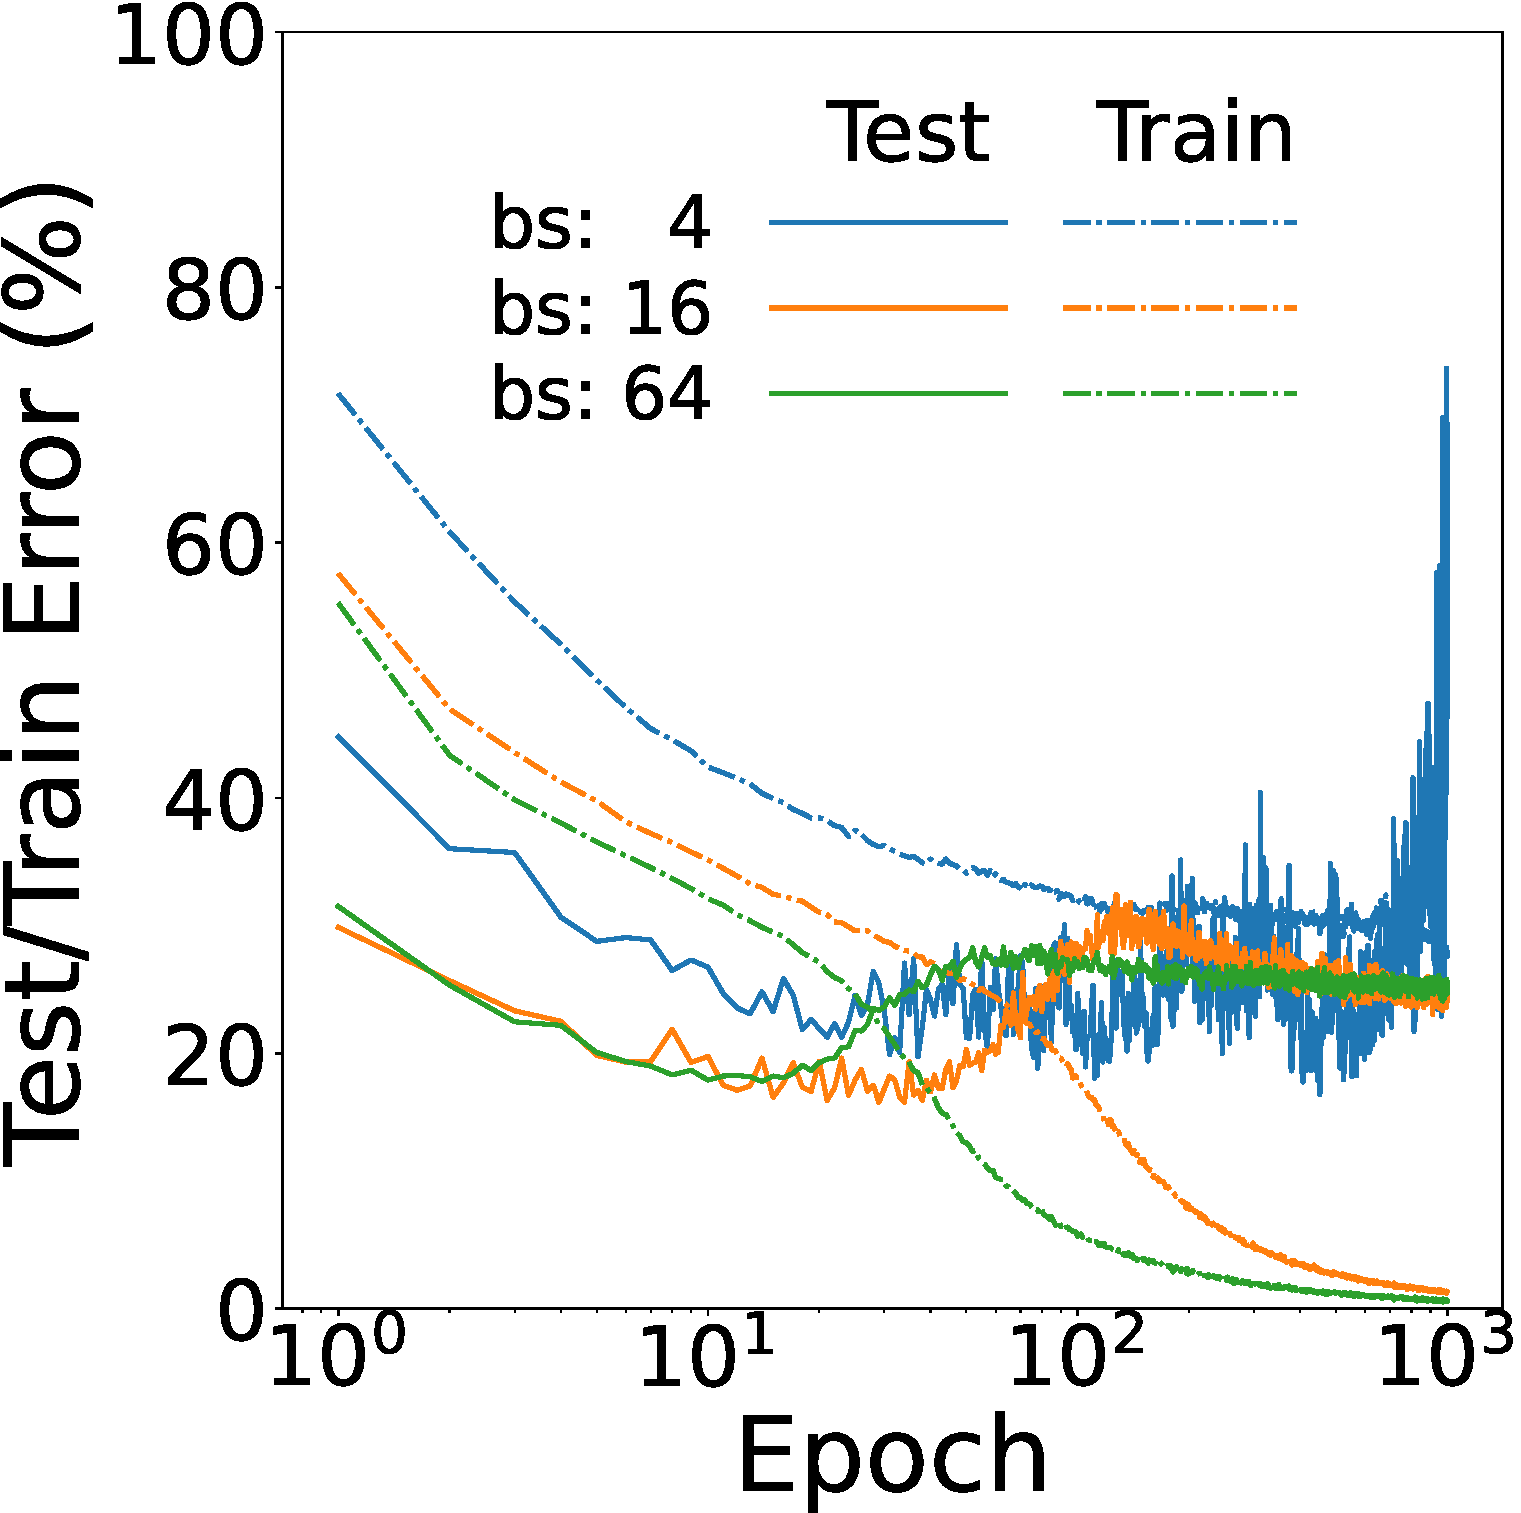
\includegraphics[keepaspectratio, width=0.45\linewidth]{fig/batchsize_learning_curv.pdf} &
        \hspace{5pt} 
      %---- 2番目の図 --------------------------
      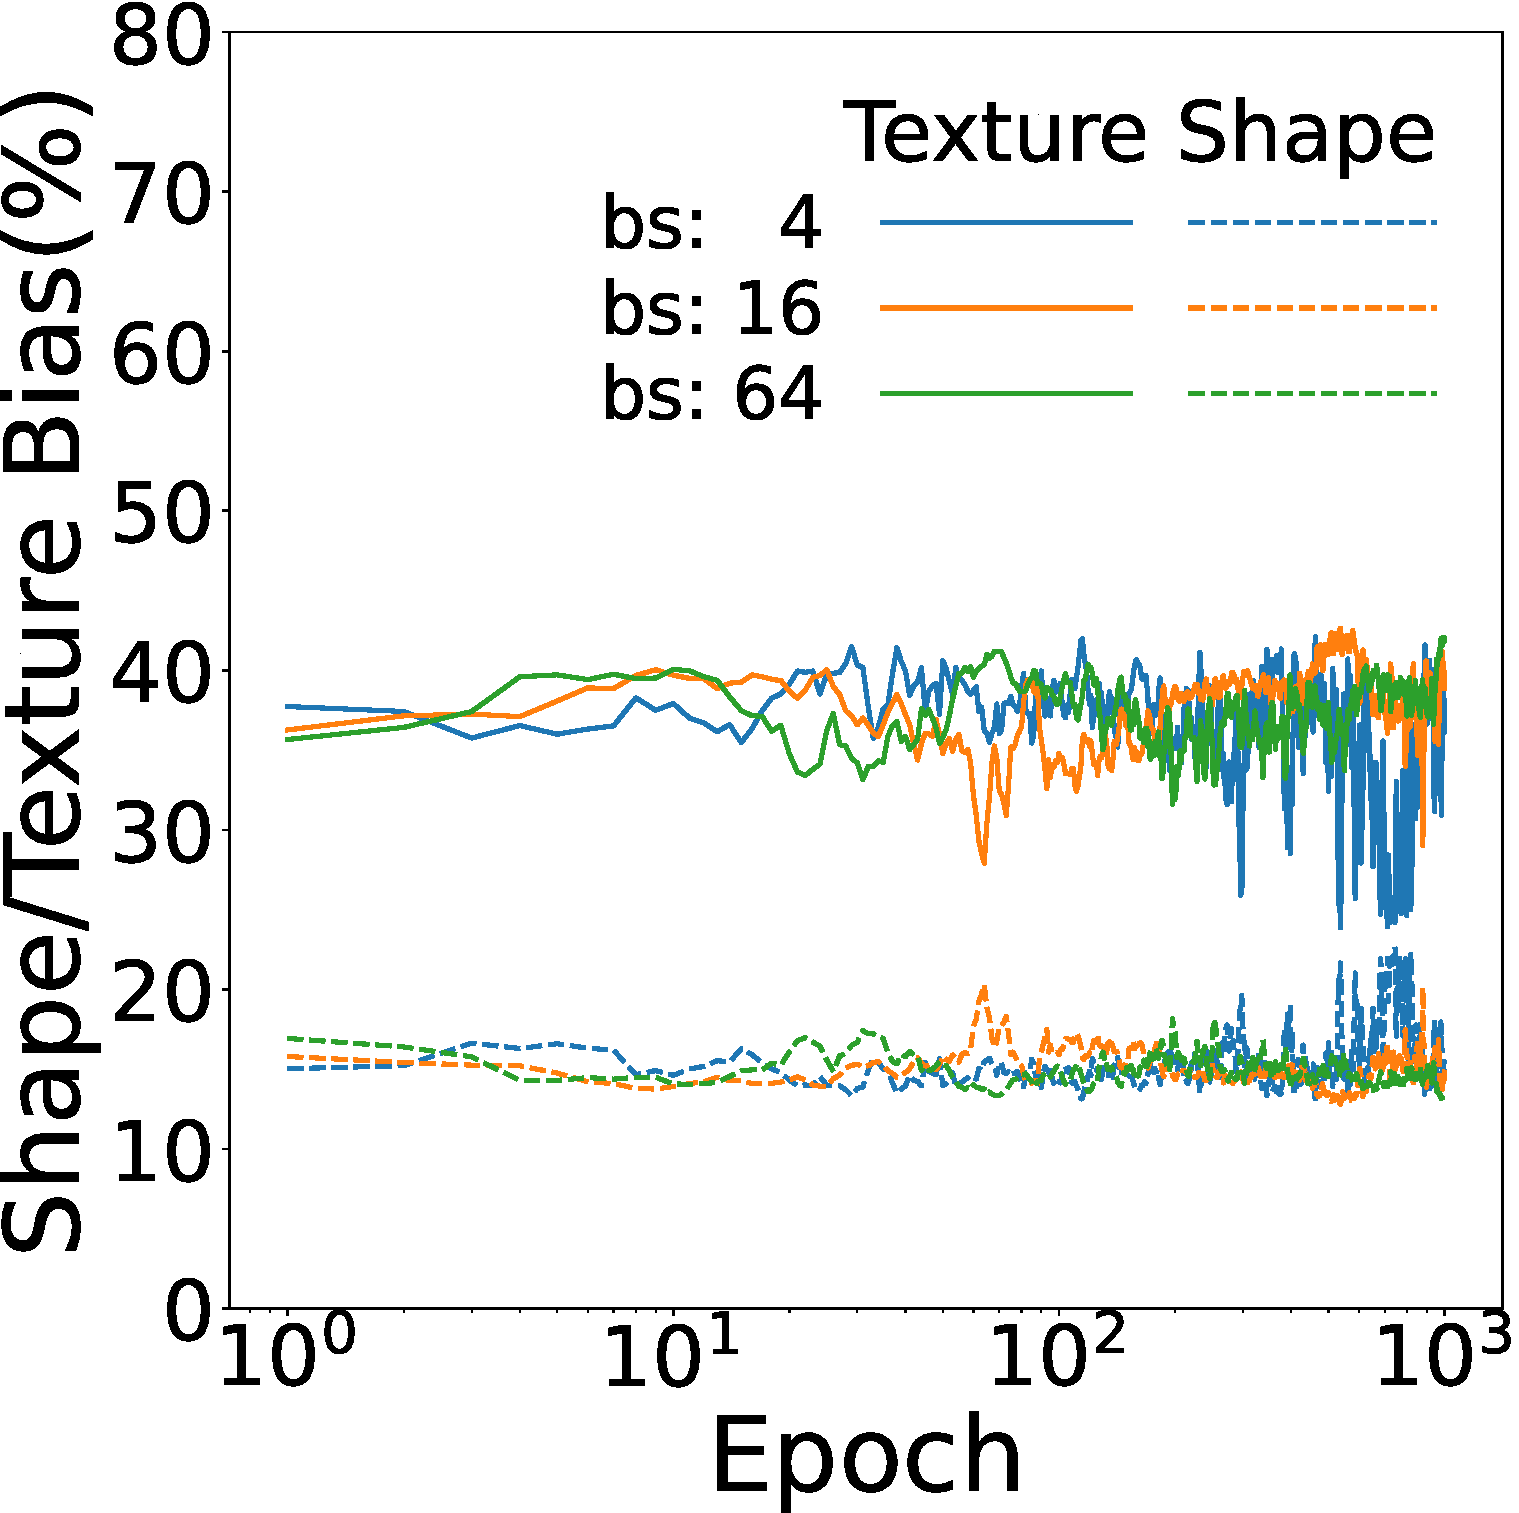
\includegraphics[keepaspectratio, width=0.45\linewidth]{fig/batchsize_sha_tex.pdf}
   \end{tabular}
\caption[Learning process under various batch size conditions.]{Learning process under various batch size conditions. Left: train/test errors Right: shape/texture bias values.}
%Learning curve graphs for double descent and shape/texture bias for different label noise. \textbf{Left}:learning curve. \textbf{Right}:model's bias shift.}
\label{fig:comp_batchsize}
\end{figure}

\begin{table}[htb]
    \centering
    \caption{
    % sample
    Correlation coefficients and scores in Phase 1, 2 and Phase 3 for different CNN models.
    }
    \scalebox{1.2}{
    \begin{tabular}{c|SSc|SSc} 
    \toprule[0.8pt]
    \multirow{2}{*}{batch size}  &  \multicolumn{3}{c|}{Correlation of Phase1,2} &  \multicolumn{3}{c}{Correlation of Phase3}\\
     \cline{2-7}
             & {SB} & {TB} & Score & {SB} & {TB} & Score \\
     \midrule[0.5pt]
    4 & N/A & N/A & N/A & N/A & N/A & N/A \\
    16 &0.249&-0.206 & 0.227 &-0.186&0.154 & 0.170\\
    64 &0.090&-0.065 & 0.077 &0.108&-0.101 & 0.105\\
    \toprule[0.8pt]
    \end{tabular}
    }
    \label{tab:corr_batchsize}
\end{table}

\newpage

\subsection[Label Noise]{Label Noise (see \cref{fig:comp_ln} and \cref{tab:corr_ln})}

ラベルノイズの増加は,二重降下の観測において重要なパラメータの一つである.そのため,特に偏重度の推移に対して,どのような影響を与えるか,ラベルノイズの割合を変更し検証を行った.ラベルノイズの増加による,二重降下と形状・テクスチャ偏重度の推移への影響を検証した結果を\cref{fig:comp_ln}に示す.ラベルノイズの割合は,20\%に加えて,40\%,60\%と変化させた条件で行った.相関係数の定量評価を\cref{tab:corr_ln}に示す.テスト誤り率の推移からわかるように,ラベルノイズが大きくなるにつれて二重降下のPhase2における変動幅が大きくなっている.しかし,形状とテクスチャ偏重度を見ると,ラベルノイズの割合に関係なく,形状・テクスチャ偏重度の明確な傾向が観察される.特に,テクスチャ偏重度では,ラベルノイズが大きくなるにつれて,上昇から下降へのシフトのタイミングが遅れているように見える.各条件の相関を比較すると,40\%の場合には相関は見られていないが,60\%の場合はScoreが0.579と,相関がみられている.このことから,ラベルノイズが大きくなるにつれて,偏重度の推移が遅くなる可能性がある.

\begin{figure}[htb]
\centering
   \begin{tabular}{cc}
      %---- 最初の図 ---------------------------
      \hspace{-5mm}
      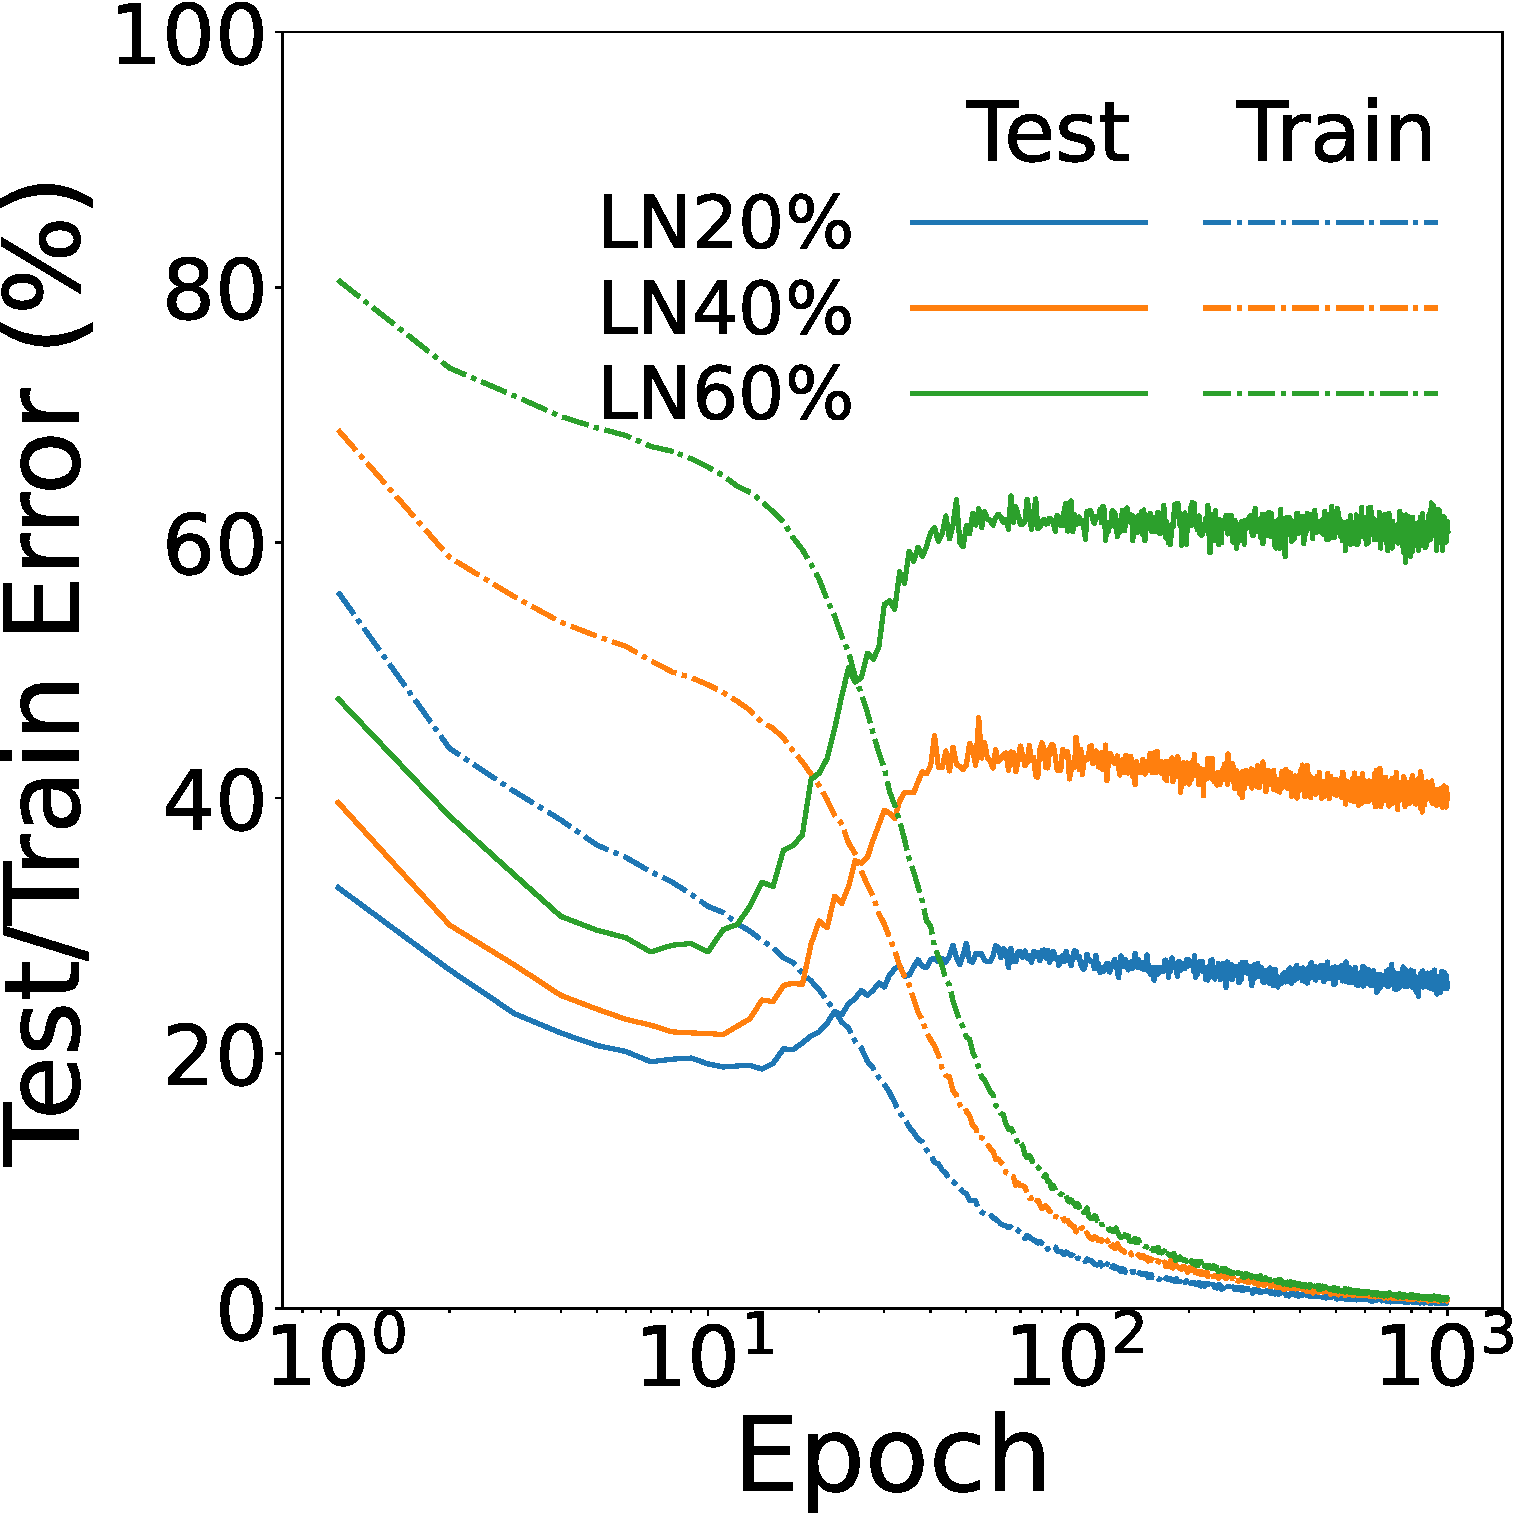
\includegraphics[keepaspectratio, width=0.45\linewidth]{fig/ln_learning_curv.pdf} &
       \hspace{5pt} 
      %---- 2番目の図 --------------------------
      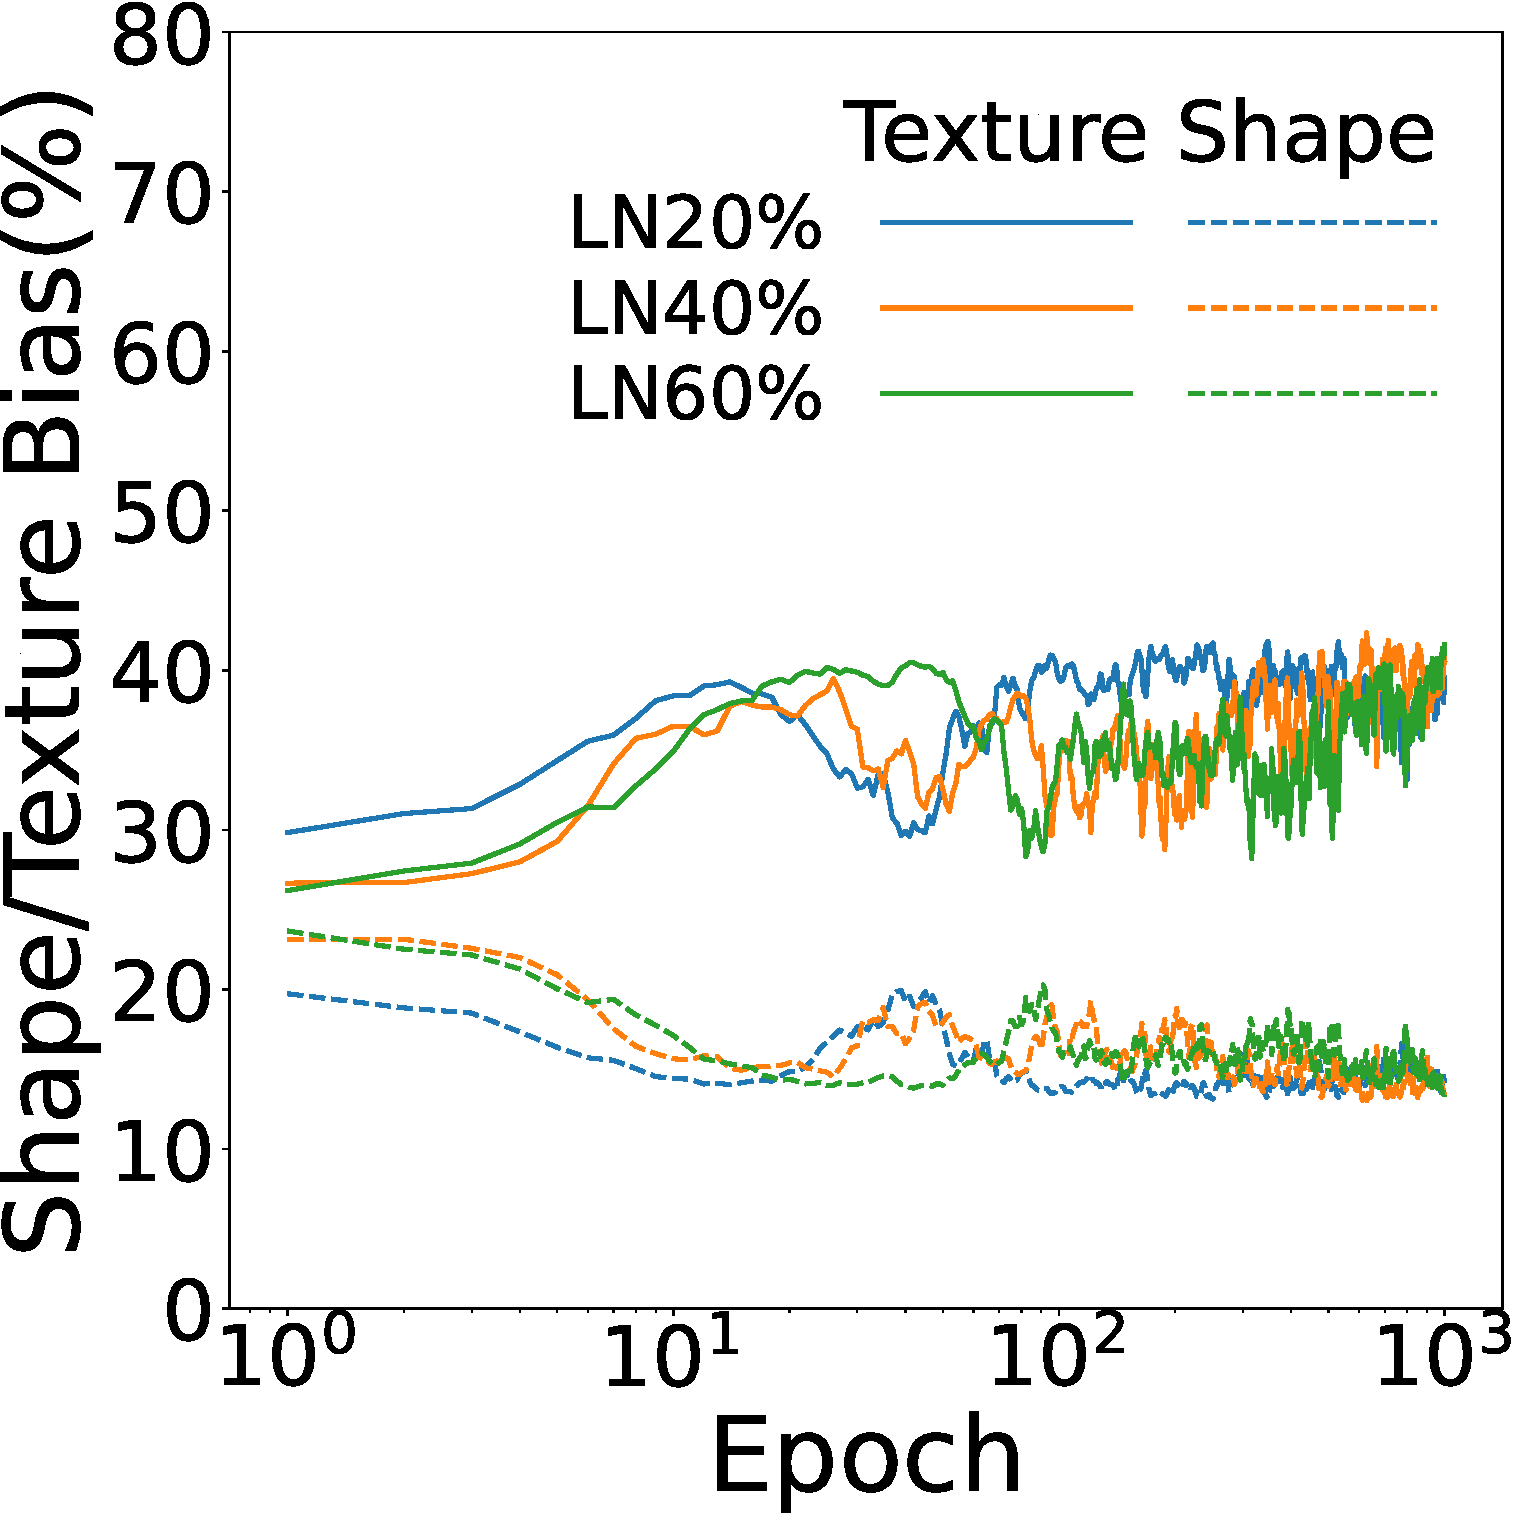
\includegraphics[keepaspectratio, width=0.45\linewidth]{fig/ln_sha_tex.pdf}
   \end{tabular}
\caption[Learning process under various label noise conditions.]{Learning process under various label noise conditions. Left: train/test errors Right: shape/texture bias values.}
%Learning curve graphs for double descent and shape/texture bias for different label noise. \textbf{Left}:learning curve. \textbf{Right}:model's bias shift.}
\label{fig:comp_ln}
\end{figure}

\begin{table}[htb]
    \centering
    \caption[Correlation coefficients and scores in Phase 1, 2 and Phase 3 on different label noise.]{
    % 異なるラベルノイズに対するPhase1,Phase2,Phase3の相関係数とスコア.テスト誤差と形状・テクスチャの偏りの相関係数(SB, TB)と,これら2つの相関係数から計算されたスコアを示す.
    Correlation coefficients and scores in Phase 1, 2 and Phase 3 on different label noise. It shows the correlation coefficients (SB, TB) between test error and shape/texture bias and the score calculated from these two correlation coefficients.
    }
    % \begin{tabular}{c|c|c} 
    % \toprule[0.8pt]
    % Label noise  & Correlation area &  score\\
    %  \midrule[0.5pt]
    % 20\%  & Stage1,2 (2-41) &0.778\\
    % 40\% & Stage1,2 (2-114) &0.048\\
    % 60\% & Stage1,2 (2-36) &0.579\\
    % \toprule[0.8pt]
    % \end{tabular}
    \scalebox{1.2}{
    \begin{tabular}{c|SSc|SSc} 
    \toprule[0.8pt]
    \multirow{2}{*}{Label Noise}  &  \multicolumn{3}{c|}{Correlation of Phase1,2} &  \multicolumn{3}{c}{Correlation of Phase3}\\
     \cline{2-7}
             & {SB} & {TB} & Score & {SB} & {TB} & Score \\
     \midrule[0.5pt]
    20\% &0.778&-0.778 & 0.778 & -0.026&0.118 & 0.072\\
    40\% & 0.004 & -0.091 & 0.048 &0.451&-0.487 & 0.469\\
    60\% &-0.560 & 0.598 & 0.579 & 0.122 & -0.142 & 0.132\\
    \toprule[0.8pt]
    \end{tabular}
    }
    \label{tab:corr_ln}
\end{table}

\newpage

\subsection[Seed]{Seed (see \cref{fig:comp_seed} and \cref{tab:corr_seed})}
機械学習の実験においては,再現性を担保するために,シード値を固定して,実験を行う場合がある.そのため,シード値を変更した場合における二重降下と形状・テクスチャ偏重度の推移への影響を検証した.使用したシード値は,元の条件である42に加えて0,1を使用した.0,1,42は機械学習の分野においてもっともよく使用されるシード値である.シード値を変更した場合の結果を\cref{fig:comp_seed}に,定量的な評価のための表を\cref{tab:corr_seed}に示す.シード値が42の場合において,ベースラインの結果と異なっているが,異なる計算機環境で実験で行った結果であることに留意されたい.
すべての場合において,二重降下がほとんど一致している.一方で,例えばテクスチャ偏重度は,すべての条件において,上昇して下降する傾向が見られる.しかし,定量的には,すべての条件において二重降下と形状・テクスチャ偏重度との相関は捉えられなかった.

事前学習したパラメータを使用する場合,事前学習をしたパラメータを読み込んだのちに,モデルが持つ全結合層のみ再度の初期化を行うことが一般的である.この実験では,シード値を変更しているが,畳み込み層は事前学習したパラメータを使用しているため,モデルが持つ全結合層のパラメータのみに差異があると考えられる.そのため,全結合層におけるパラメータの初期値が,二重降下にはさほど影響を与えないが,偏重度の推移には大きく影響を与えていると推察される.

\begin{figure}[htb]
\centering
   \begin{tabular}{cc}
      %---- 最初の図 ---------------------------
      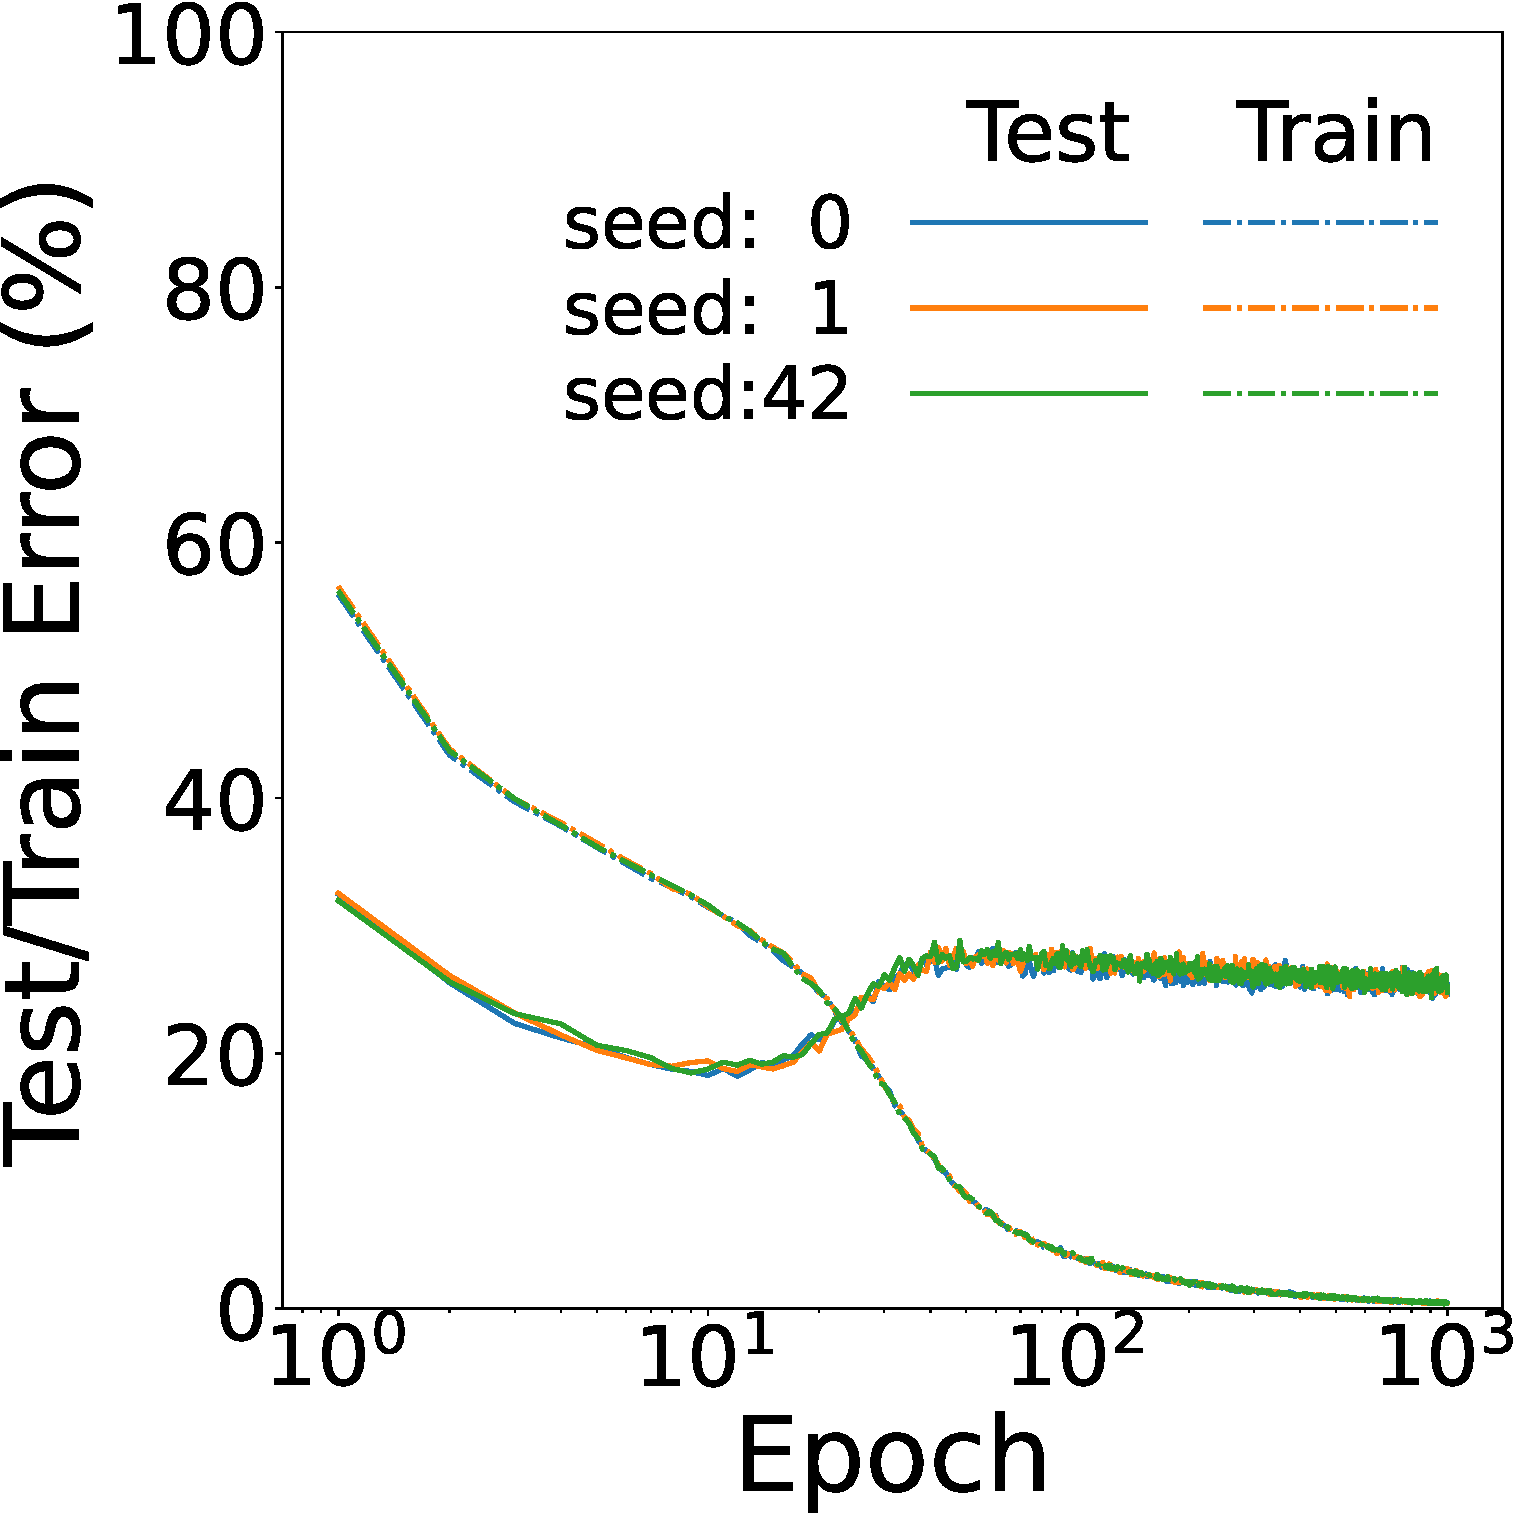
\includegraphics[keepaspectratio, width=0.45\linewidth]{fig/seed_learning_curv.pdf} &
       \hspace{5pt} 
      %---- 2番目の図 --------------------------
      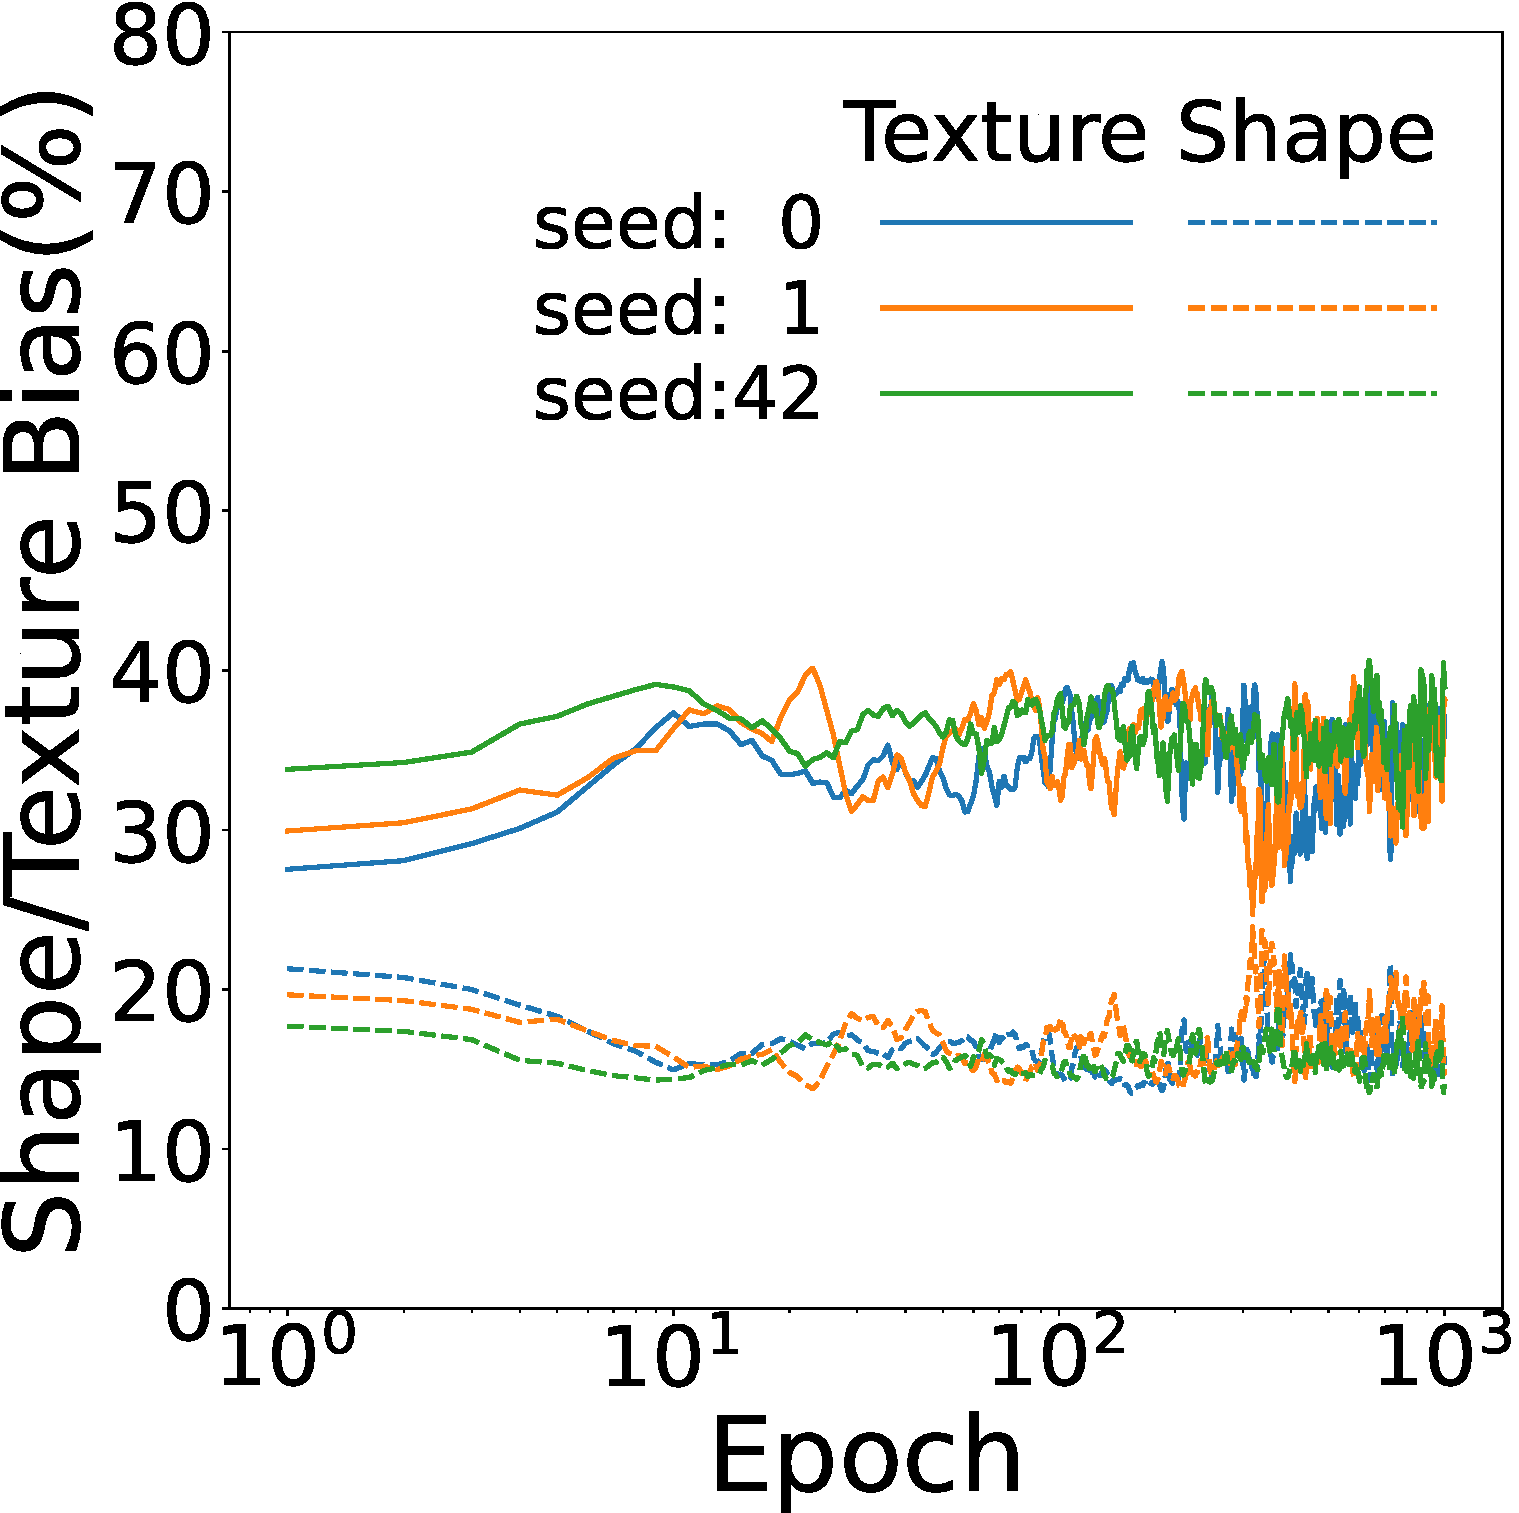
\includegraphics[keepaspectratio, width=0.45\linewidth]{fig/seed_sha_tex.pdf}
   \end{tabular}
\caption[Learning process under various seed conditions.]{Learning process under various seed conditions. Left: train/test errors Right: shape/texture bias values.}
%Learning curve graphs for double descent and shape/texture bias for different label noise. \textbf{Left}:learning curve. \textbf{Right}:model's bias shift.}
\label{fig:comp_seed}
\end{figure}

\newpage

\begin{table}[htb]
    \centering
    \caption[Correlation coefficients and scores in Phase 1, 2 and Phase 3 under various seed conditions.]{
    % 異なるラベルノイズに対するPhase1,Phase2,Phase3の相関係数とスコア.テスト誤差と形状・テクスチャの偏りの相関係数(SB, TB)と,これら2つの相関係数から計算されたスコアを示す.
    Correlation coefficients and scores in Phase 1, 2 and Phase 3 on different label noise. It shows the correlation coefficients (SB, TB) between test error and shape/texture bias and the score calculated from these two correlation coefficients.
    }
    % \begin{tabular}{c|c|c} 
    % \toprule[0.8pt]
    % Label noise  & Correlation area &  score\\
    %  \midrule[0.5pt]
    % 20\%  & Stage1,2 (2-41) &0.778\\
    % 40\% & Stage1,2 (2-114) &0.048\\
    % 60\% & Stage1,2 (2-36) &0.579\\
    % \toprule[0.8pt]
    % \end{tabular}
    \scalebox{1.2}{
    \begin{tabular}{c|SSc|SSc} 
    \toprule[0.8pt]
    \multirow{2}{*}{Seed}  &  \multicolumn{3}{c|}{Correlation of Phase1,2} &  \multicolumn{3}{c}{Correlation of Phase3}\\
     \cline{2-7}
             & {SB} & {TB} & Score & {SB} & {TB} & Score \\
     \midrule[0.5pt]
    0 &0.034&-0.178 & 0.105 & -0.132& 0.133 & 0.132\\
    1 & 0.040 & -0.013 & 0.026 &-0.123&0.087 & 0.105\\
    42 &-0.015 & -0.087 & 0.051 & 0.069 & 0.017 & 0.043\\
    \toprule[0.8pt]
    \end{tabular}
    }
    \label{tab:corr_seed}
\end{table}

\newpage

% \chapter{層ごとの学習過程に着目した検証}
\section{はじめに}
Heckelらは,モデルの異なる部分が異なるエポックで学習とし,層ごとに学習率を変更することで二重降下が緩和することを示している\cite{Heckel}.本章では,\cref{fig:overview}を観察した条件において,層ごとの特徴学習過程に着目した複数の検証を行う.今後の実験の理解を助けるために,ResNet18の構造を説明する.Heらの論文のTable 1を\cref{tab:ResNet_arch}に示す.ResNet18は,大まかに,17層の畳み込み層と1層の全結合層から構成される.また最初の層を除いた畳み込み層は,4層ごとにブロックを構成している.以降では,1層目の畳み込み層をconv1,4つのブロックを浅い位置から,block1,block2,block3,block4と呼称する.

\newcommand{\blocka}[2]{\multirow{3}{*}{\(\left[\begin{array}{c}\text{3$\times$3, #1}\\[-.1em] \text{3$\times$3, #1} \end{array}\right]\)$\times$#2}
}
\newcommand{\blockb}[3]{\multirow{3}{*}{\(\left[\begin{array}{c}\text{1$\times$1, #2}\\[-.1em] \text{3$\times$3, #2}\\[-.1em] \text{1$\times$1, #1}\end{array}\right]\)$\times$#3}
}
\begin{table}[htb]
\caption{ResNet architecture (citing Tab. 1 of [10]).}
\vspace{-.5em}
\begin{center}
\resizebox{0.9\linewidth}{!}{
%\footnotesize
\begin{tabular}{c|c|c|c|c|c|c}
\hline
layer name & output size & 18-layer & 34-layer & 50-layer & 101-layer & 152-layer \\
\hline
conv1 & 112$\times$112 & \multicolumn{5}{c}{7$\times$7, 64, stride 2}\\
\hline
\multirow{4}{*}{conv2\_x} & \multirow{4}{*}{56$\times$56} & \multicolumn{5}{c}{3$\times$3 max pool, stride 2} \\\cline{3-7}
  &  & \blocka{64}{2}  & \blocka{64}{3} & \blockb{256}{64}{3} & \blockb{256}{64}{3} & \blockb{256}{64}{3}\\
  &  &  &  &  &  &\\
  &  &  &  &  &  &\\
\hline
\multirow{3}{*}{conv3\_x} &  \multirow{3}{*}{28$\times$28}  & \blocka{128}{2}  & \blocka{128}{4}  & \blockb{512}{128}{4}  & \blockb{512}{128}{4}  &
                              \blockb{512}{128}{8}\\
  &  &  &  &  &  & \\
  &  &  &  &  &  & \\
\hline
\multirow{3}{*}{conv4\_x} & \multirow{3}{*}{14$\times$14}  & \blocka{256}{2}  & \blocka{256}{6}  & \blockb{1024}{256}{6}  & \blockb{1024}{256}{23} & \blockb{1024}{256}{36}\\
  &  &  &  &  & \\
  &  &  &  &  & \\
\hline
\multirow{3}{*}{conv5\_x} & \multirow{3}{*}{7$\times$7}  & \blocka{512}{2}  & \blocka{512}{3}  & \blockb{2048}{512}{3}  & \blockb{2048}{512}{3}
& \blockb{2048}{512}{3}\\
  &  &  &  &  &  & \\
  &  &  &  &  &  & \\
\hline
& 1$\times$1  & \multicolumn{5}{c}{average pool, 1000-d fc, softmax} \\
\hline
\multicolumn{2}{c|}{FLOPs} & 1.8$\times10^9$  & 3.6$\times10^9$  & 3.8$\times10^9$  & 7.6$\times10^9$  & 11.3$\times10^9$ \\
\hline
\end{tabular}
}
\end{center}
\vspace{-.5em}
\label{tab:ResNet_arch}
\vspace{-.5em}
\end{table}

\section{階層ごとの偏重度}
本研究では,形状・テクスチャ偏重度をモデルが持つ最終畳み込み層が出力する特徴マップから算出している.しかし,\cref{sec:形状・テクスチャ偏重度の定量化}の方法を使用して,異なる層からも形状・テクスチャへの偏重度が計算可能である.そのため,今まで使用していた17層(=block4の最後の畳み込み層)に対して,各blockの最後の畳み込み層(5層,9層,13層)で形状・テクスチャへの偏重度を算出し,最後の畳み込み層から算出した形状・テクスチャ偏重度の推移と比較した.

結果を\cref{fig:layer_ab}に示す.17層においては形状・テクスチャ偏重度が特異な推移をしているのに対して,5層,9層,13層における形状・テクスチャへの偏重度の推移は基本的に一定で推移している.このことから,深い層のみで見られる特性があると考えられる.また,この特性を理解することで,二重降下に対してのより深い理解への糸口となる可能性がある.
\begin{figure}[h]
\centering
\begin{minipage}[b]{.48\linewidth}
    \centering
    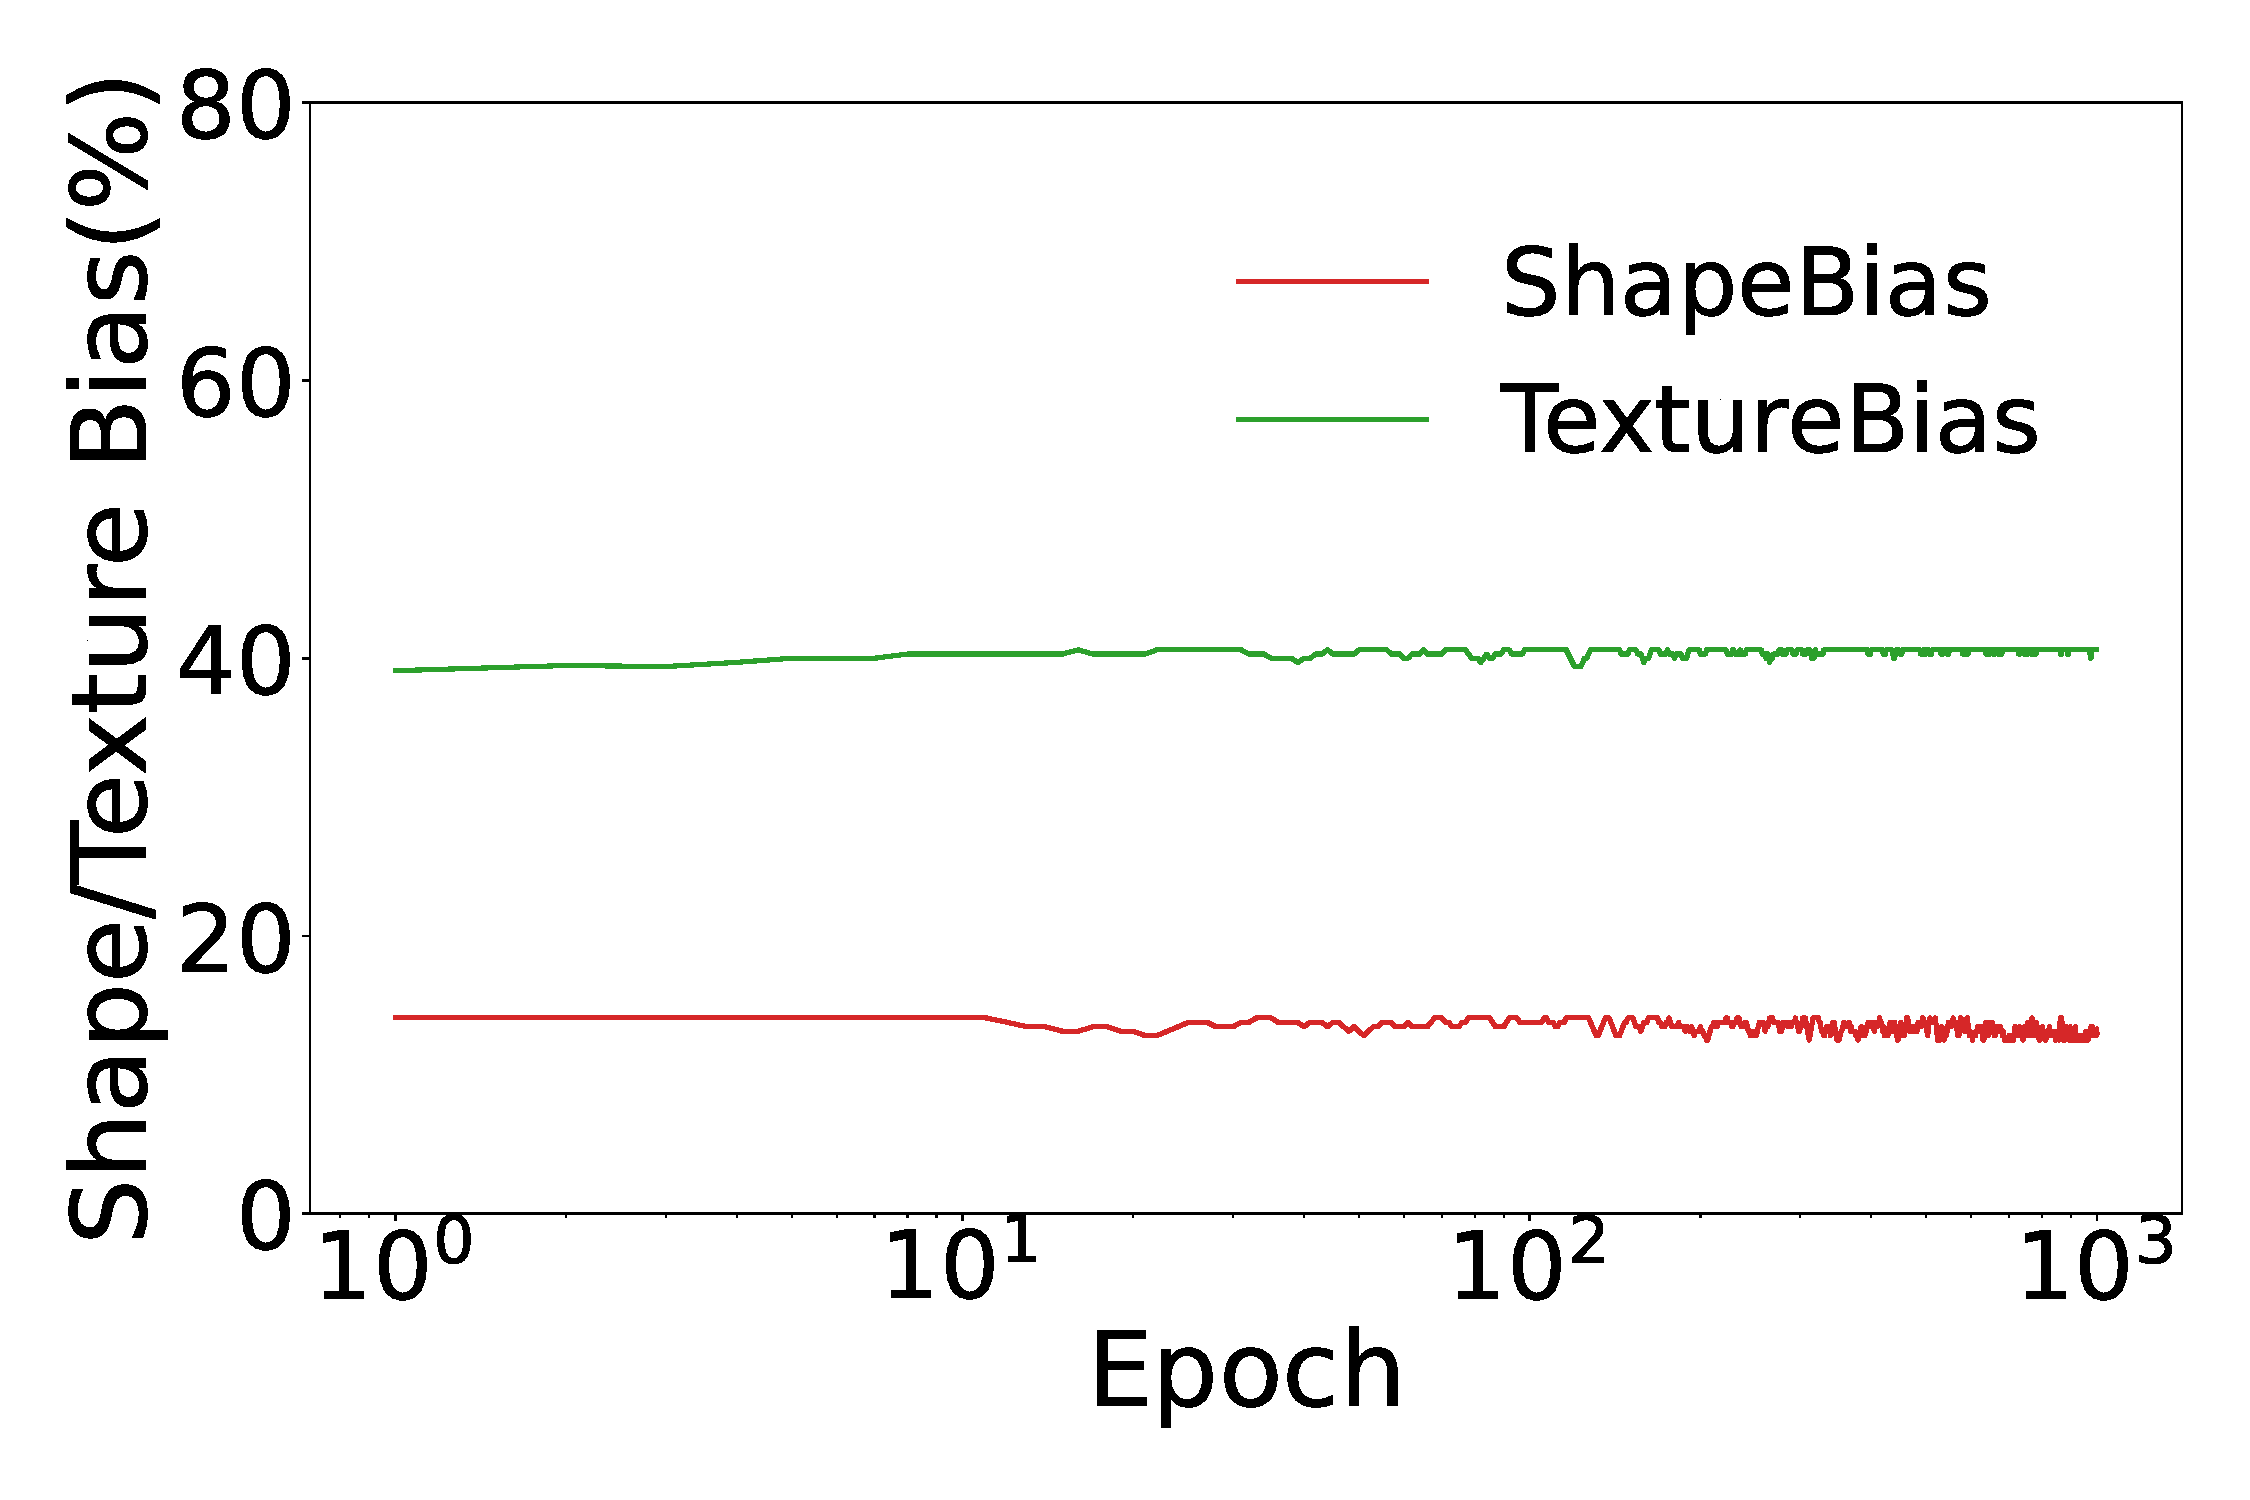
\includegraphics[width=1\linewidth]{bias_fig/IN_ResNet18/layer5.pdf}
    \subcaption{5th layer}% \caption{Figure caption}
  \end{minipage}
\begin{minipage}[b]{.48\linewidth}
    \centering
    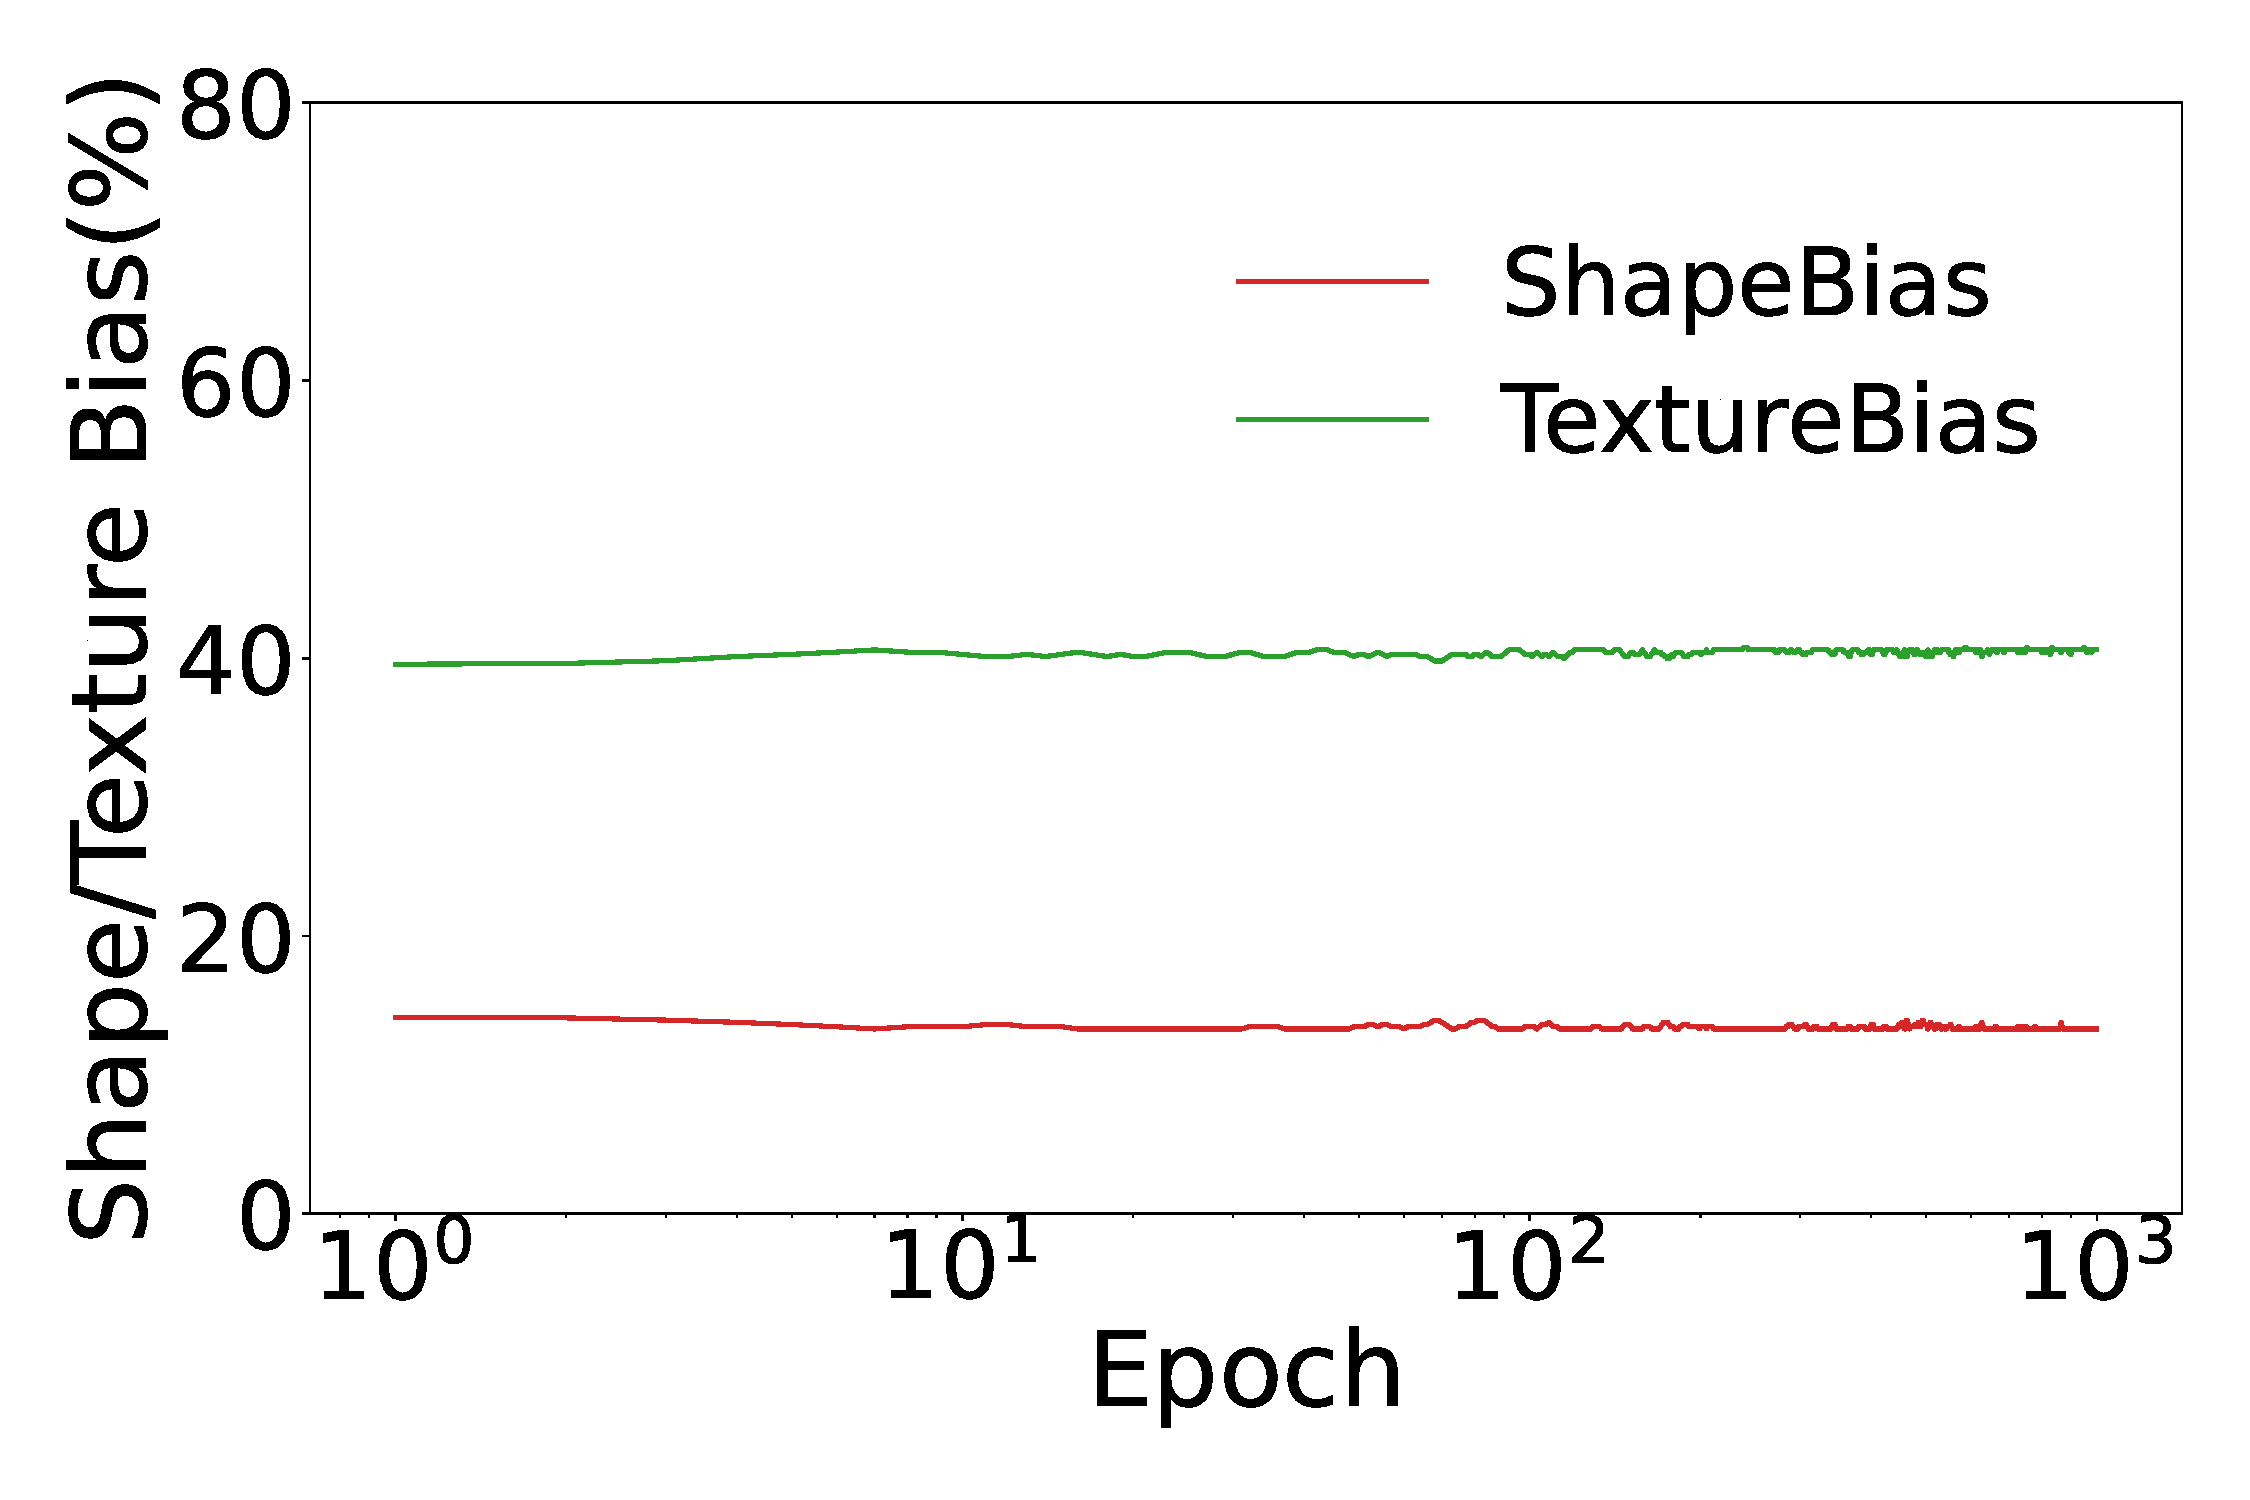
\includegraphics[width=1\linewidth]{bias_fig/IN_ResNet18/layer9.pdf}
    \subcaption{9th layer}% \caption{Figure caption}
  \end{minipage}
\begin{minipage}[b]{.48\linewidth}
    \centering
    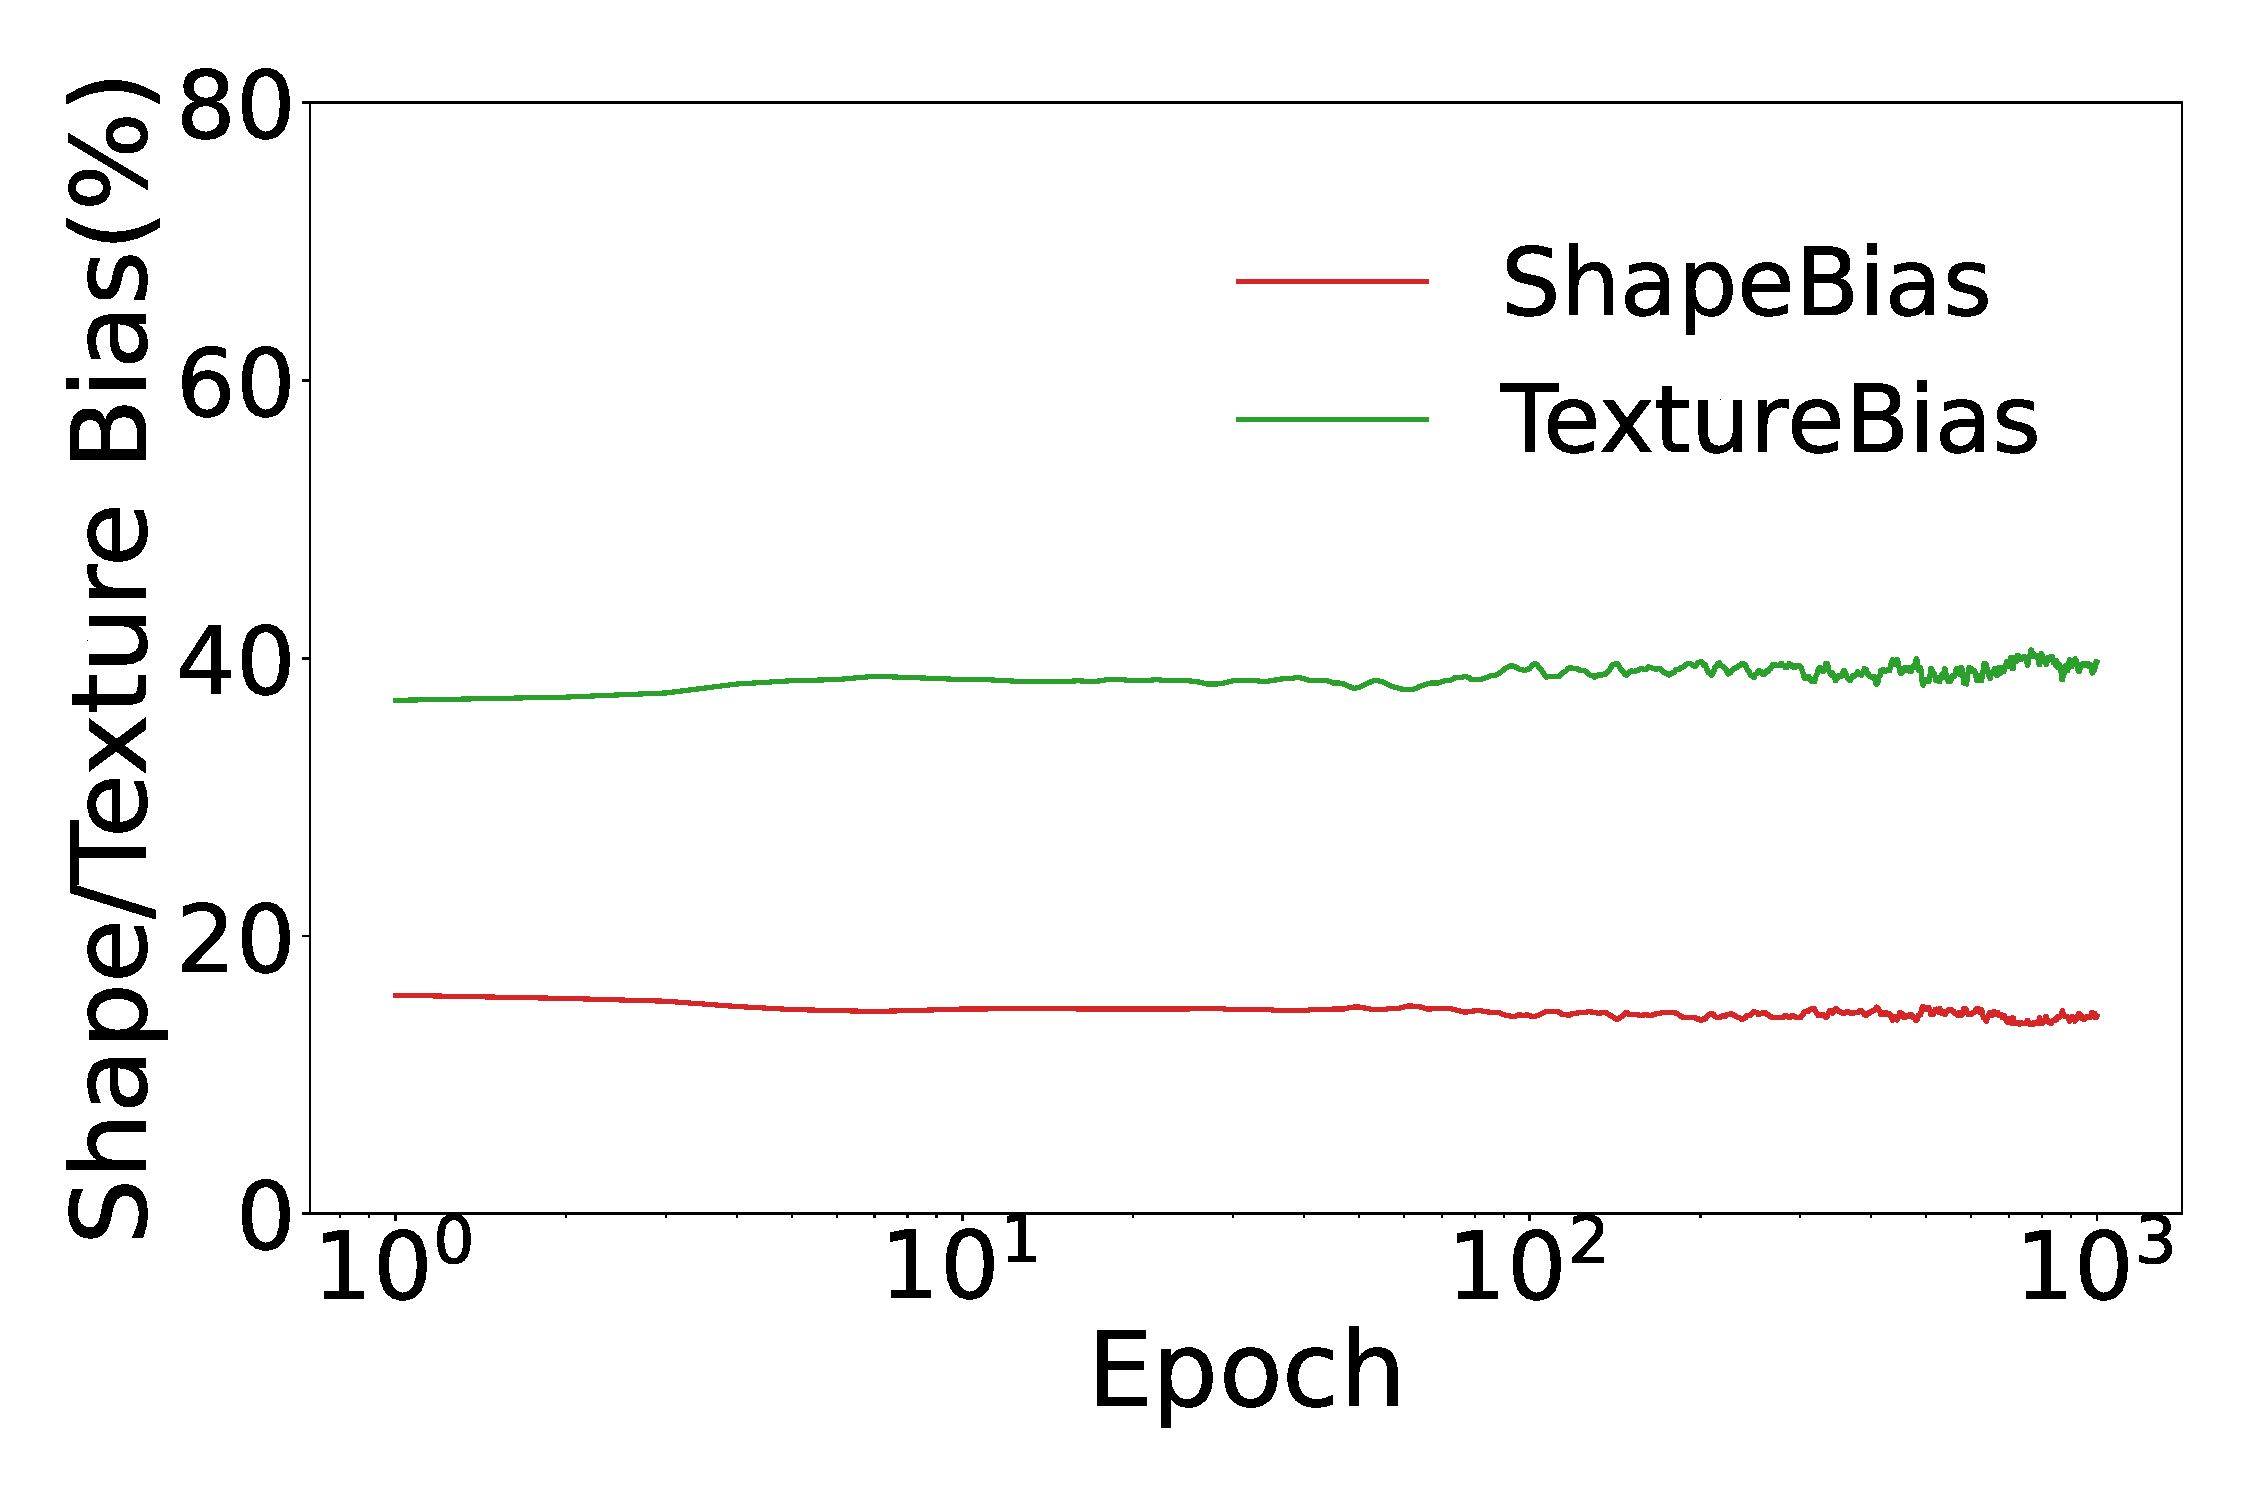
\includegraphics[width=1\linewidth]{bias_fig/IN_ResNet18/layer13.pdf}
    \subcaption{13th layer}% \caption{Figure caption}
  \end{minipage}
\begin{minipage}[b]{.48\linewidth}
    \centering
    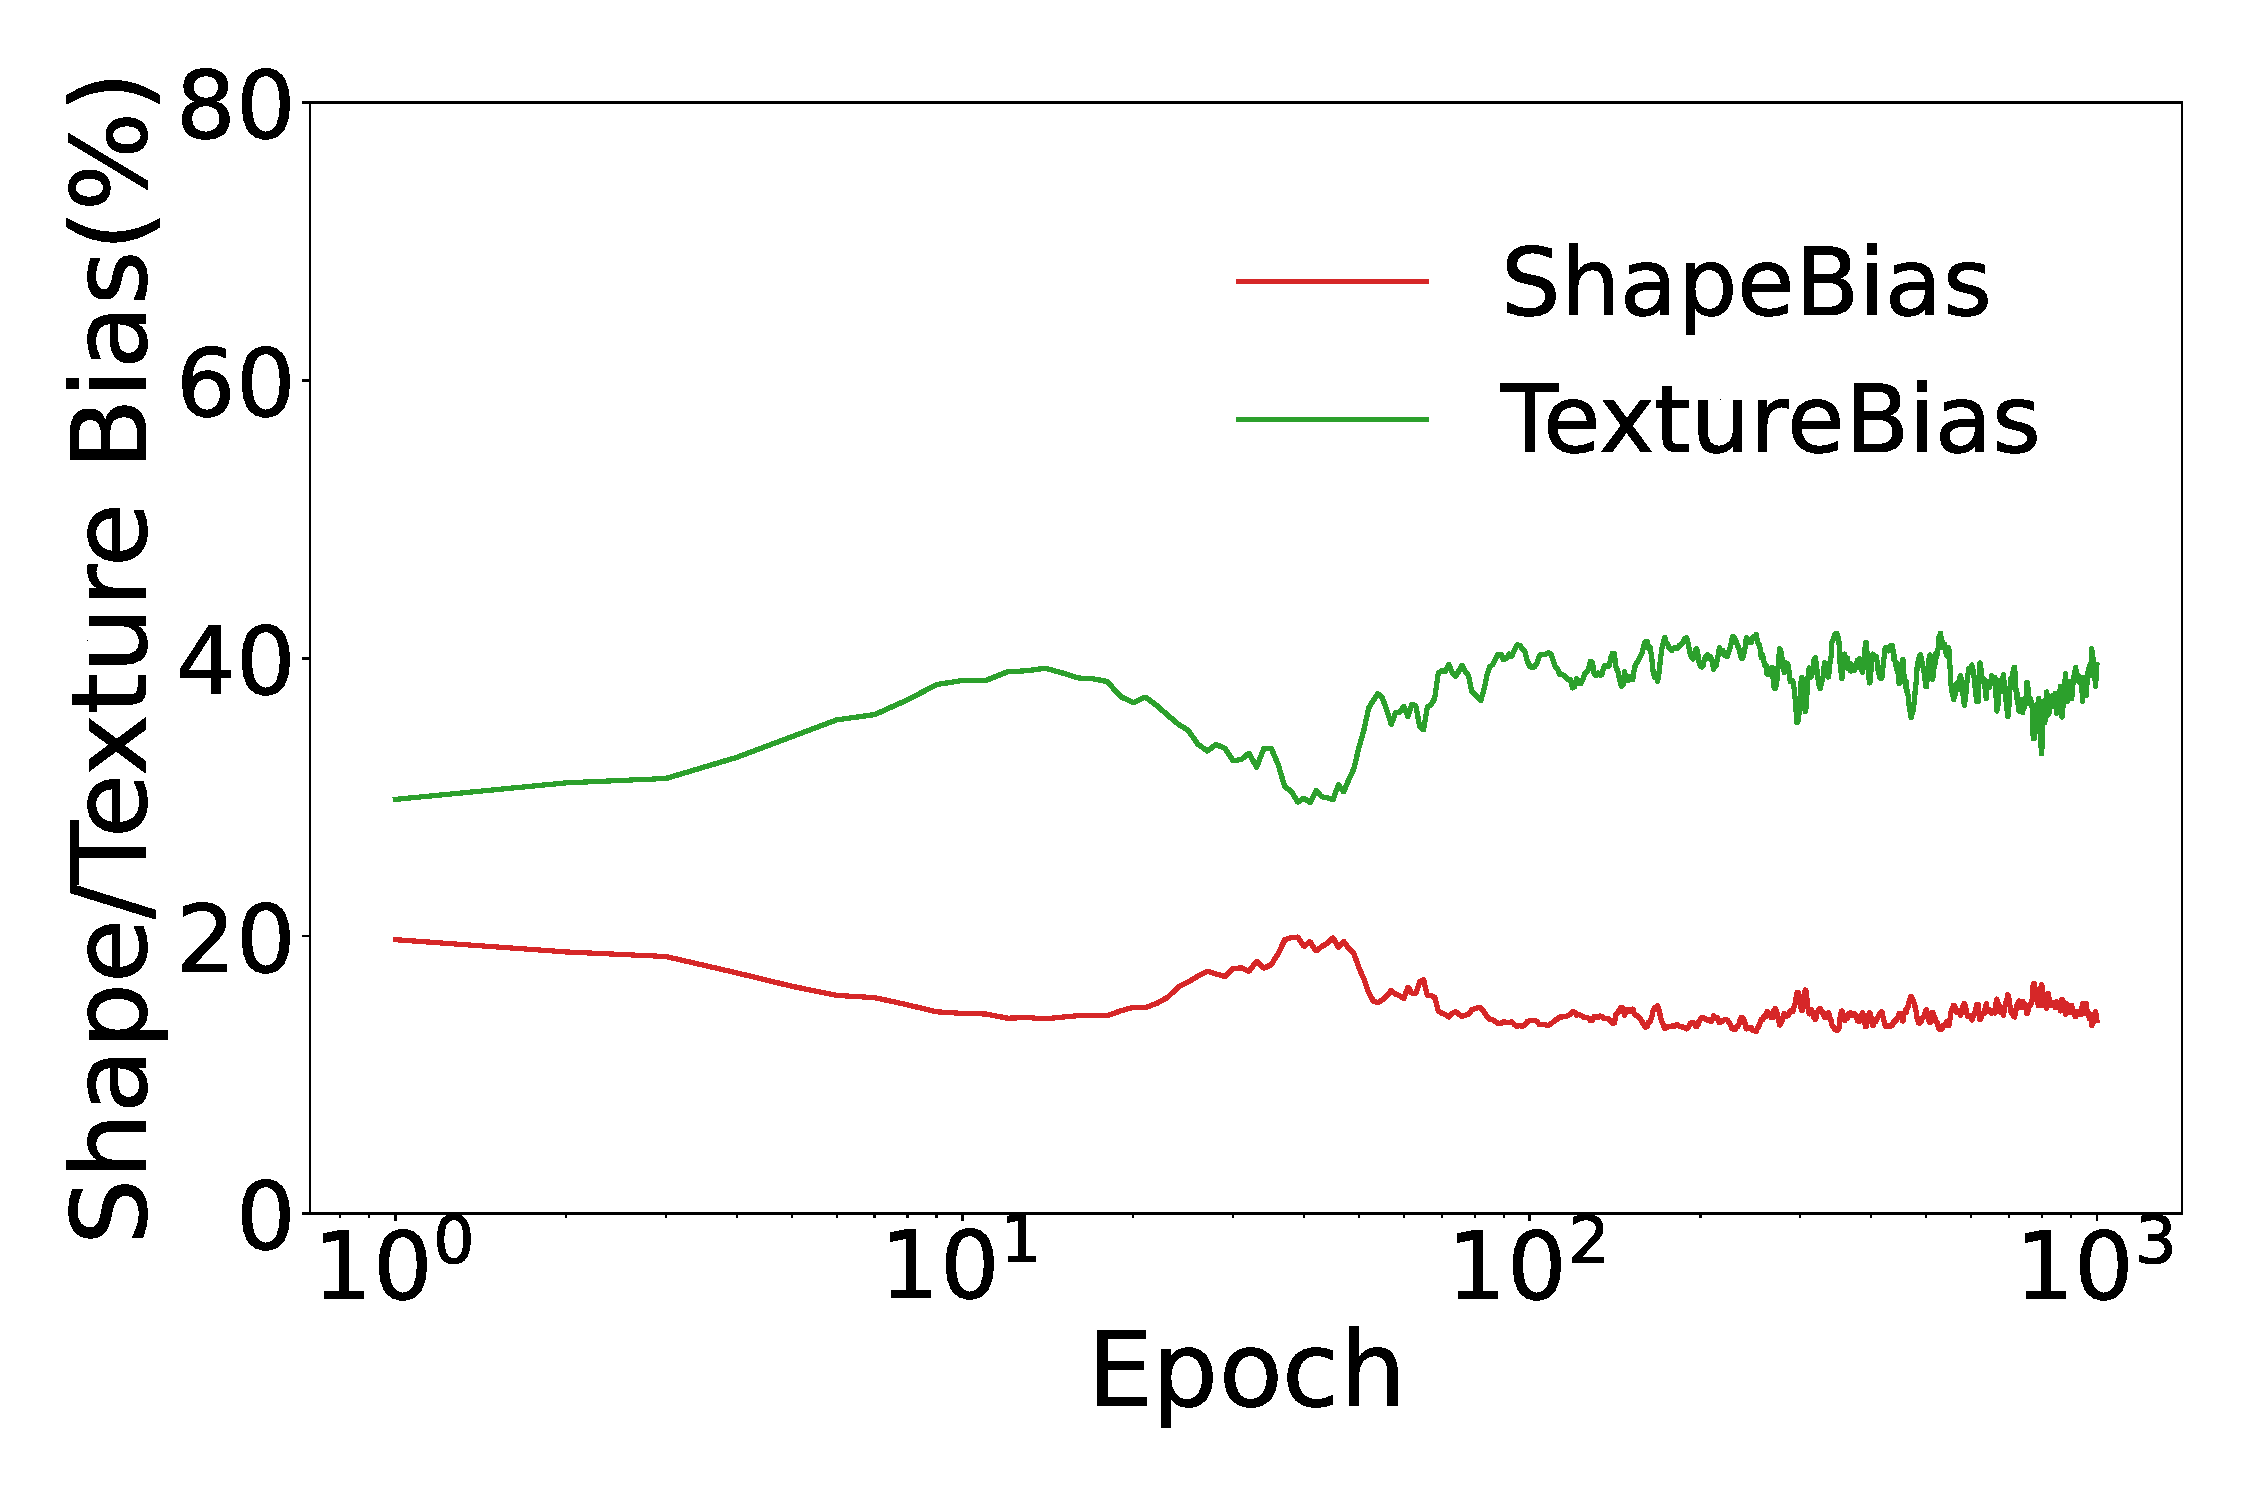
\includegraphics[width=1\linewidth]{bias_fig/IN_ResNet18/layer17.pdf}
    \subcaption{17th layer}% \caption{Figure caption}
  \end{minipage}
\caption{
The shift of biases during the learning process in each layer consisting ResNet18. 
}
\label{fig:layer_ab}
\end{figure}

\newpage

\section{浅い層のカーネル可視化}
前節では,深い層にのみ見られる何らかの特性が存在する可能性が示唆された,一方で,浅い層に変化はないのか,第1層の可視化を通して検証を行った.使用した条件は,前節と同様に,\cref{fig:overview}と同様である.二重降下の推移が切り替わる点であり,Phaseの切り替わりである13,42,そして学習が終わる1,000 epoch目において可視化を行った.

結果を\cref{fig:visualized_kernel}に示す.各フィルターを確認すると,形状テクスチャ偏重度の特異な推移が確認される条件においても,変化は微小である.浅い層の変化は少ないことから,偏重度の特異な推移に,浅い層の学習が関係している可能性は引くと考えられる.また,事前学習したときに収束したパラメータが,浅い層においては,異なるデータセット(今回はCIFAR-10)に対しても有効であったためだと考える.
\begin{figure}[h]
    \centering
    \begin{subfigure}{0.3\textwidth}
        \centering
        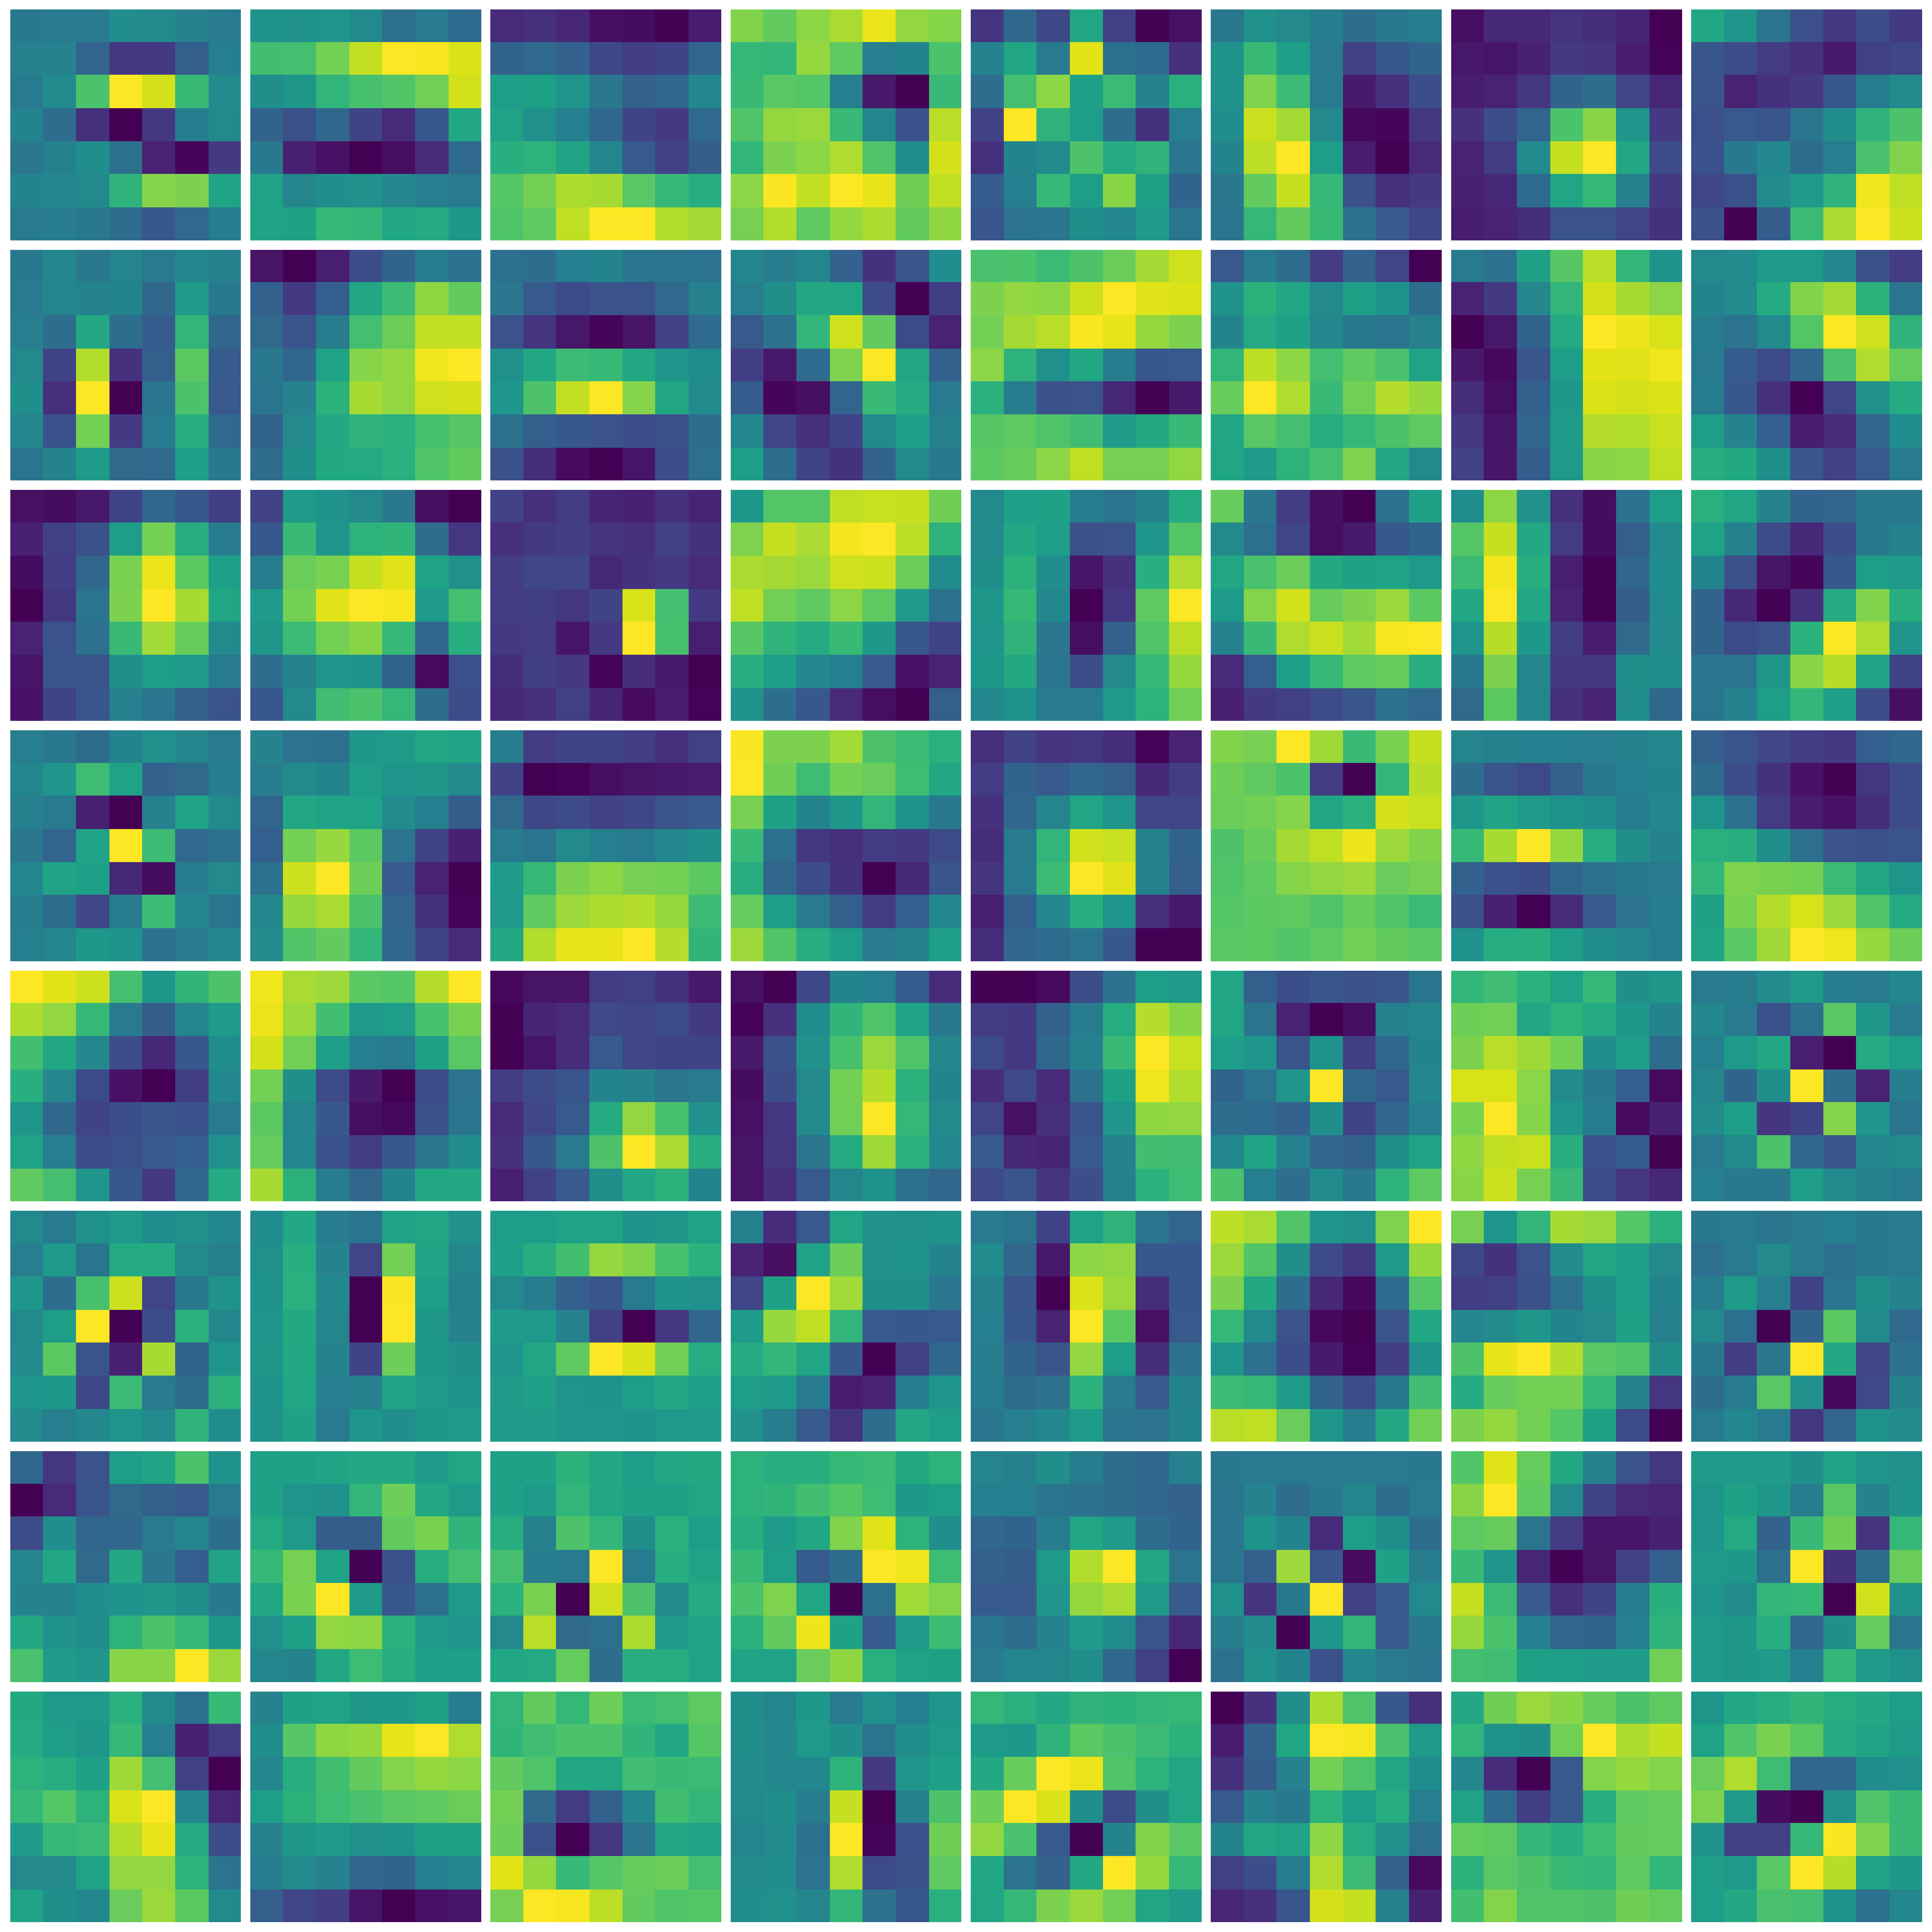
\includegraphics[width=\linewidth]{fig/IN_kernel/Visualize_epoch13.pdf}
        \caption{13th Epoch}
        \label{fig:13th}
    \end{subfigure}
    \begin{subfigure}{0.3\textwidth}
        \centering
        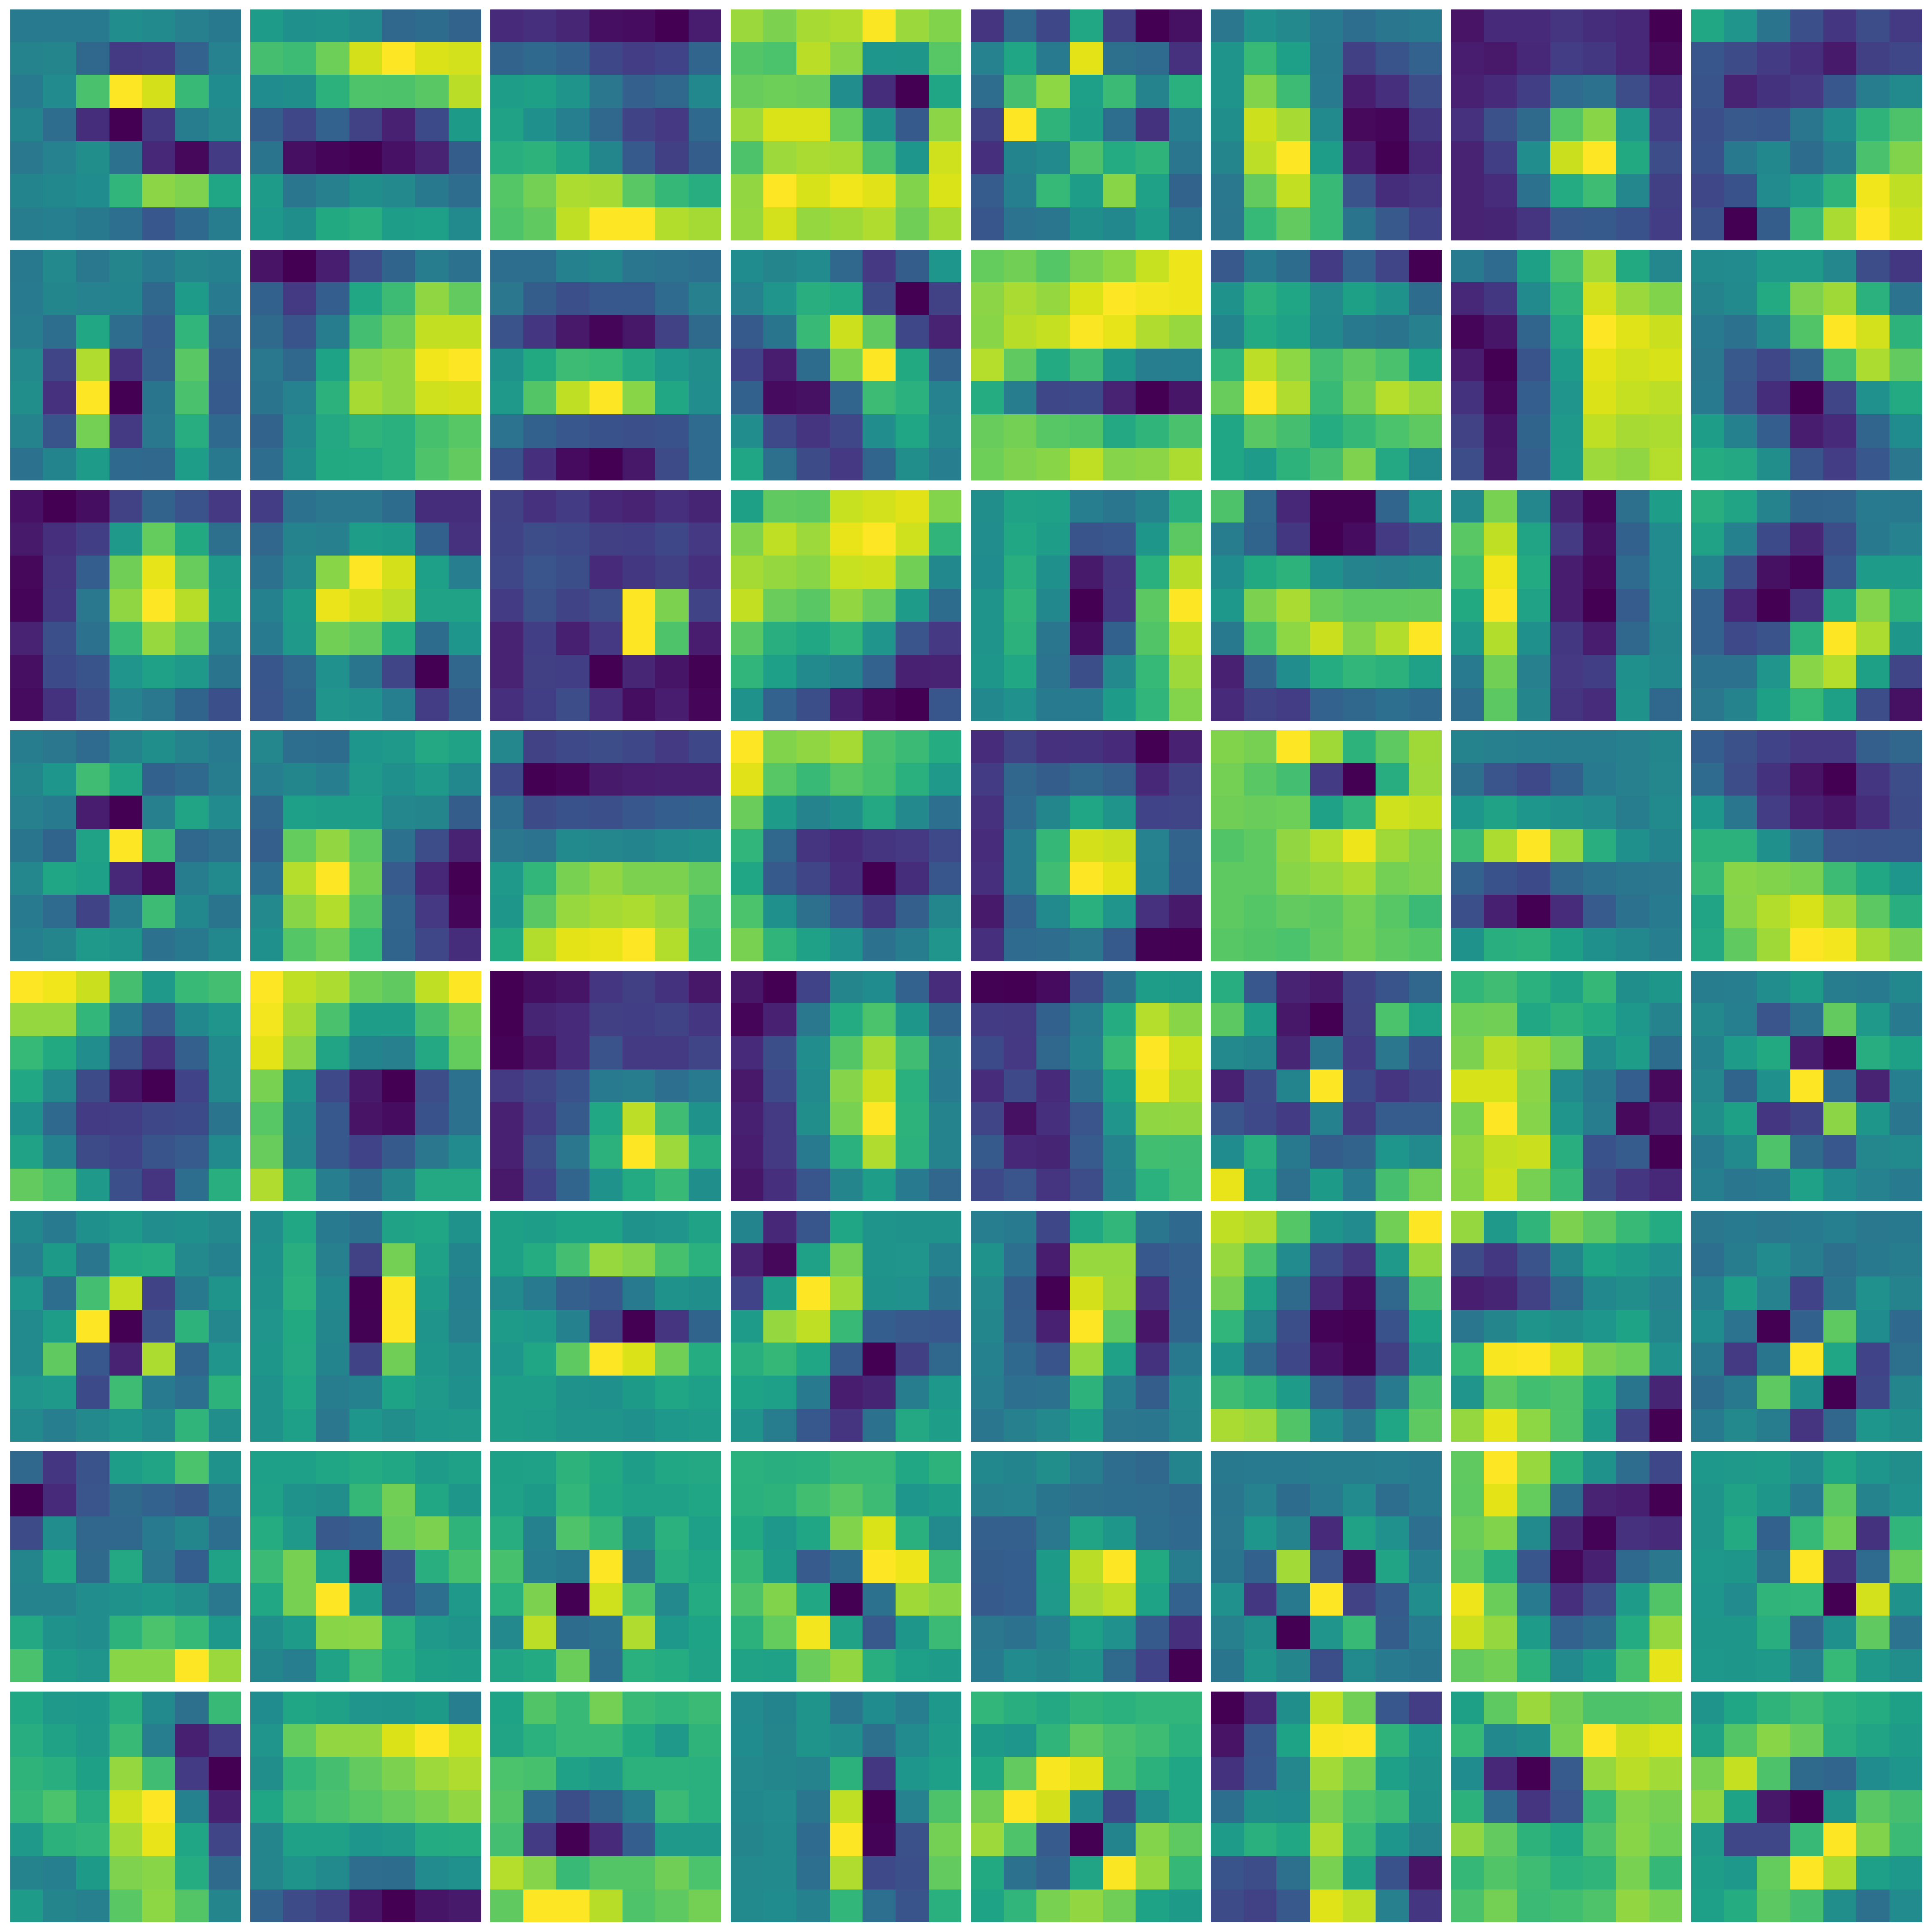
\includegraphics[width=\linewidth]{fig/IN_kernel/Visualize_epoch42.pdf}
        \caption{42nd Epoch}
        \label{fig:42nd}
    \end{subfigure}
    \begin{subfigure}{0.3\textwidth}
        \centering
        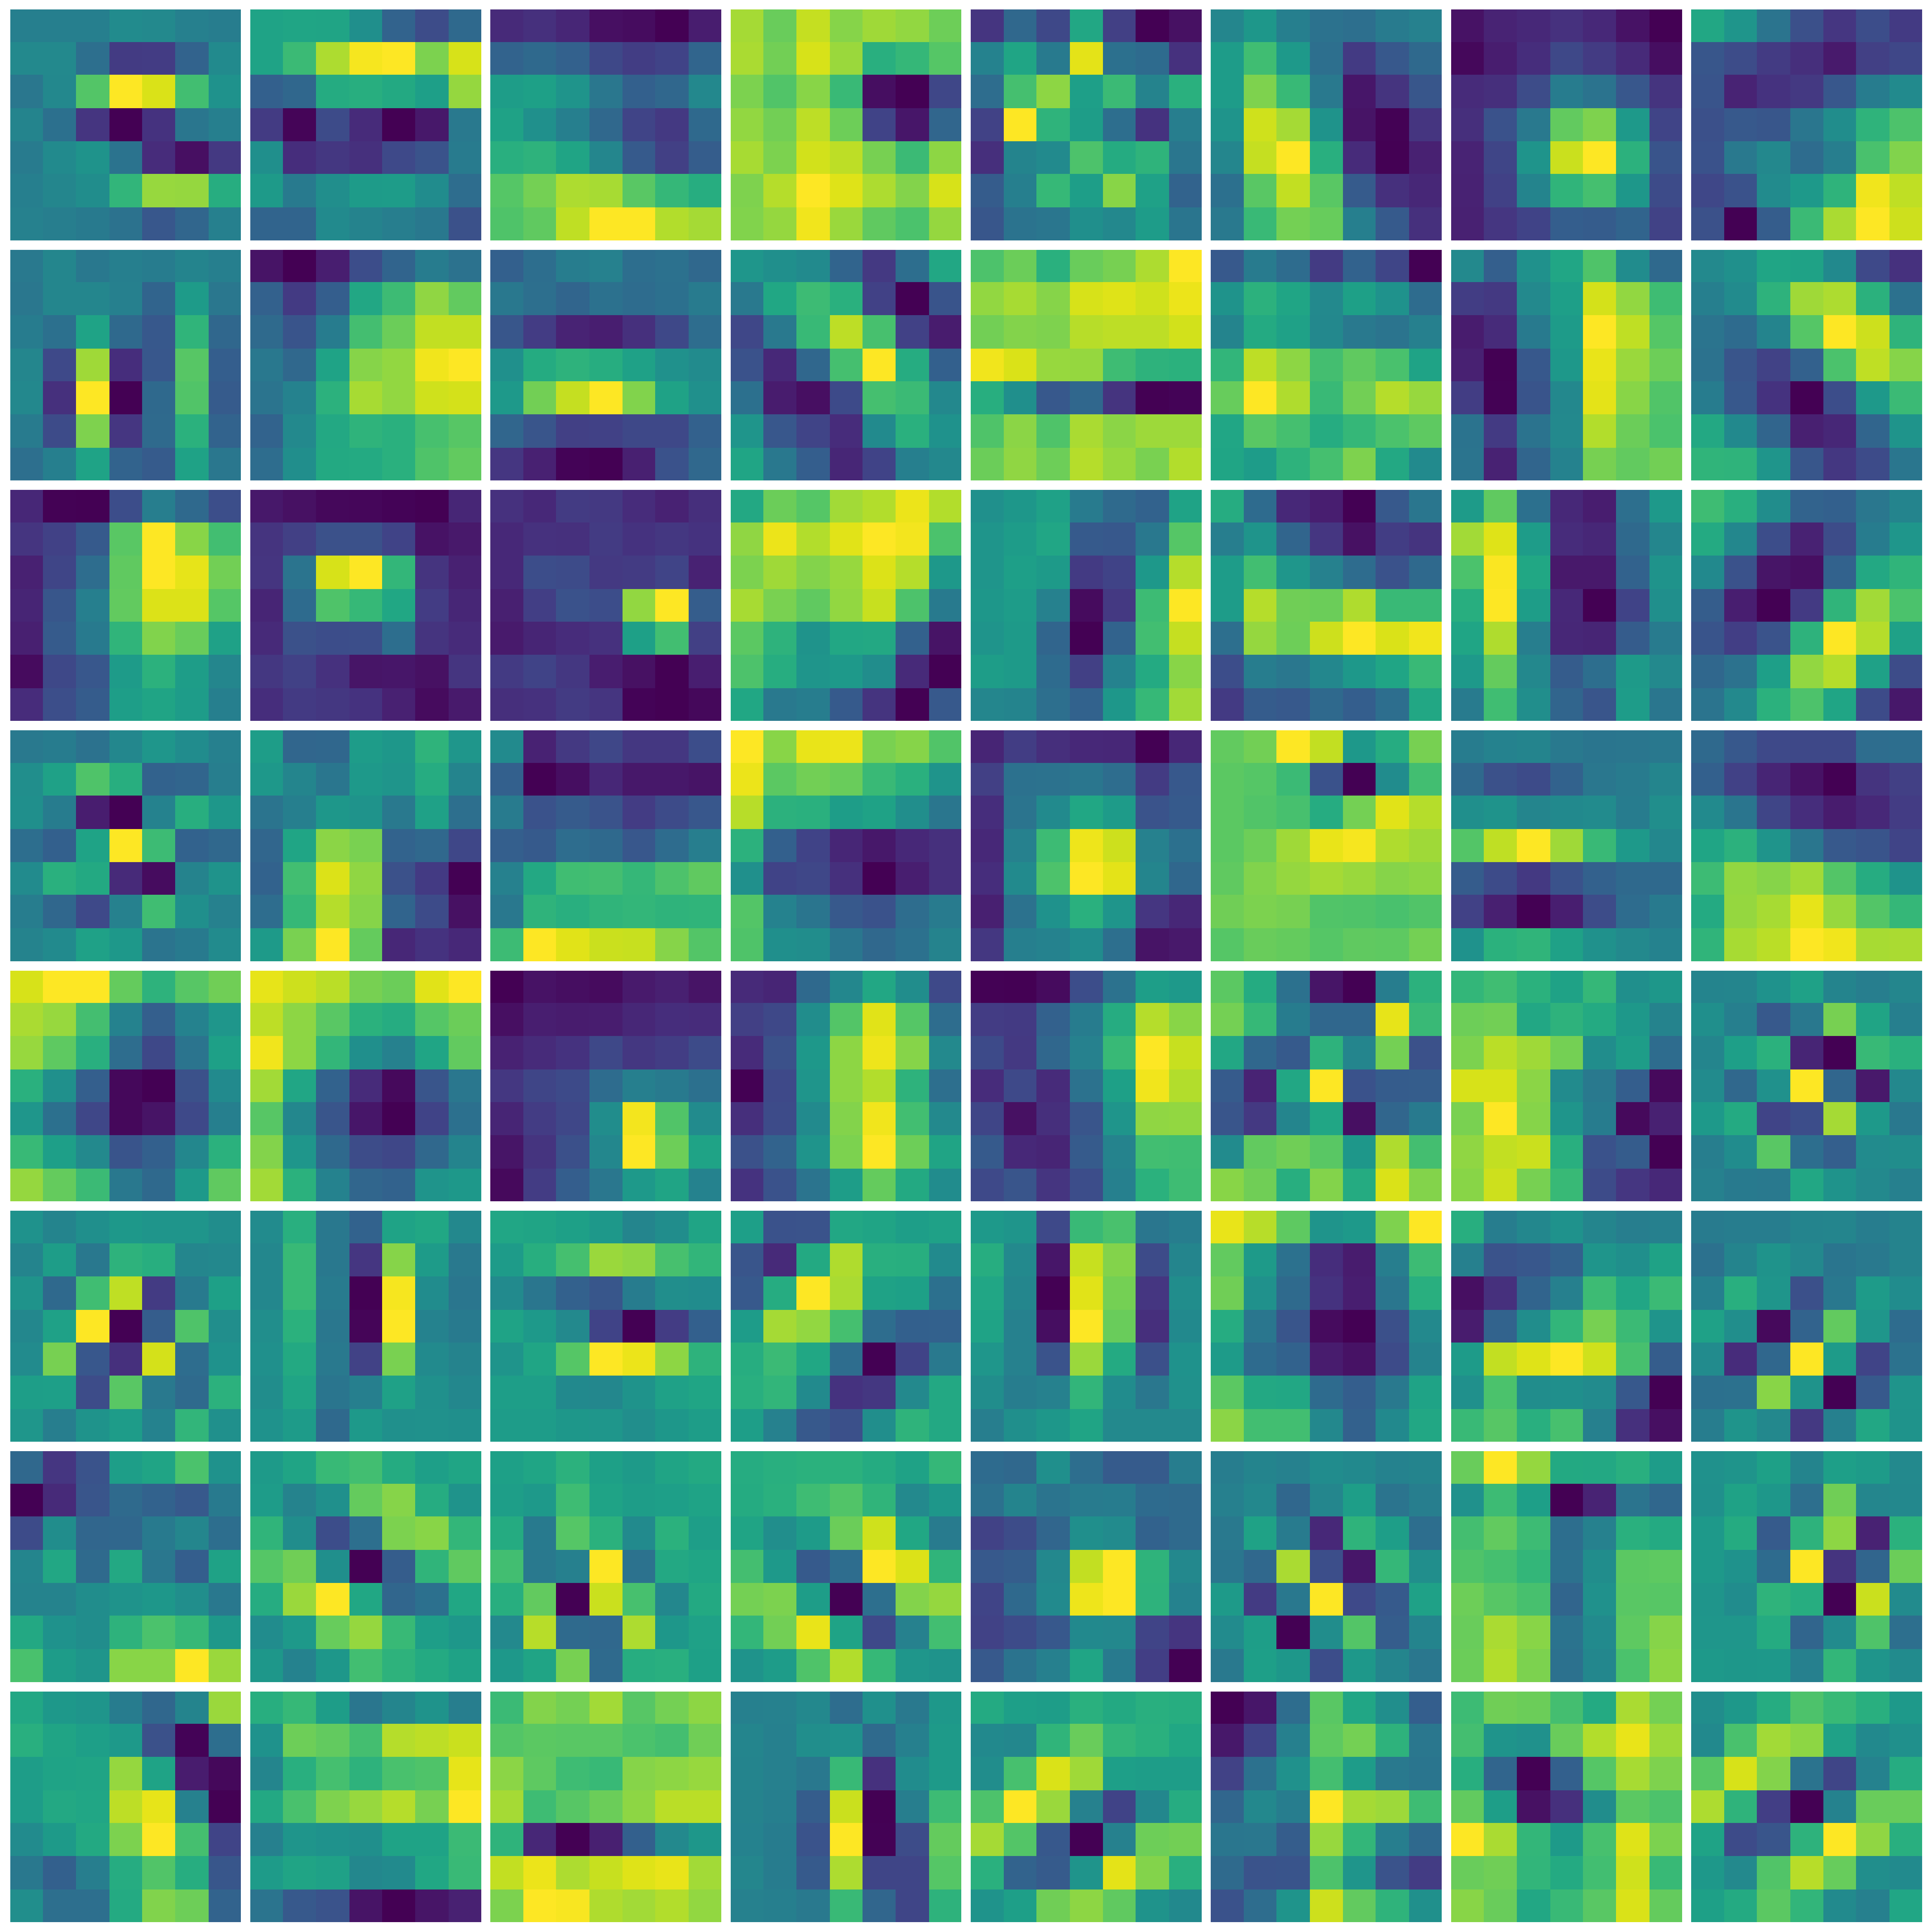
\includegraphics[width=\linewidth]{fig/IN_kernel/Visualize_epoch1000.pdf}
        \caption{1,000th Epoch}
        \label{fig:1000th}
    \end{subfigure}
    \caption[Visualization of the 1st layer in the learning process.]{
    % 学習過程における1st layerの可視化.\cref{sec:Experimental setting}で説明した設定において,二重降下を3つのPhaseに分割するEpoch(13th, 42nd Epoch),1,000th Epochにおける1st layerを可視化している.
    Visualization of the 1st layer in the learning process. In the setting described in Sec. 5.2, we visualize the 1st layer in the Epoch (13th, 42nd Epoch) and the 1,000th Epoch, where the double descent is divided into 3 Phases. The 1st layer at the 1,000th Epoch is visualized.
    }
    \label{fig:visualized_kernel}
\end{figure}

\newpage

\section{ブロック凍結実験}
深い層,浅い層における学習時の性質がそれぞれ二重降下と形状テクスチャ偏重度にどのように影響するかを観察するため,モデルが持つパラメータを凍結して,\cref{fig:overview}と同様に実験を行った.パラメータの凍結は,指定した層のパラメータを更新しないというものである.
深い層から順に凍結した場合の結果を\cref{fig:comp_frozen_deep_layer}に示す.深い層から凍結するパラメータを増加させていくと,二重降下の曲線は著しく変化が見られる.それに対して,形状テクスチャ偏重度は,特にfcからblock3を凍結した場合に,二重降下の下降から上昇に移り変わる部分と同期しているように見られる.
浅い層から順に凍結した場合の結果を\cref{fig:comp_frozen_shallow_layer}に示す.この場合は二重降下の曲線はほぼ一致しており,形状・テクスチャ偏重度の推移も類似点が確認できる.
このような結果から,深い層のパラメータが学習される場合,浅い層よりも,二重降下などに対して強い影響を与えていると考えられる.

\begin{figure}[htb]
\centering
   \begin{tabular}{cc}
      %---- 最初の図 ---------------------------
      \hspace{-5mm}
      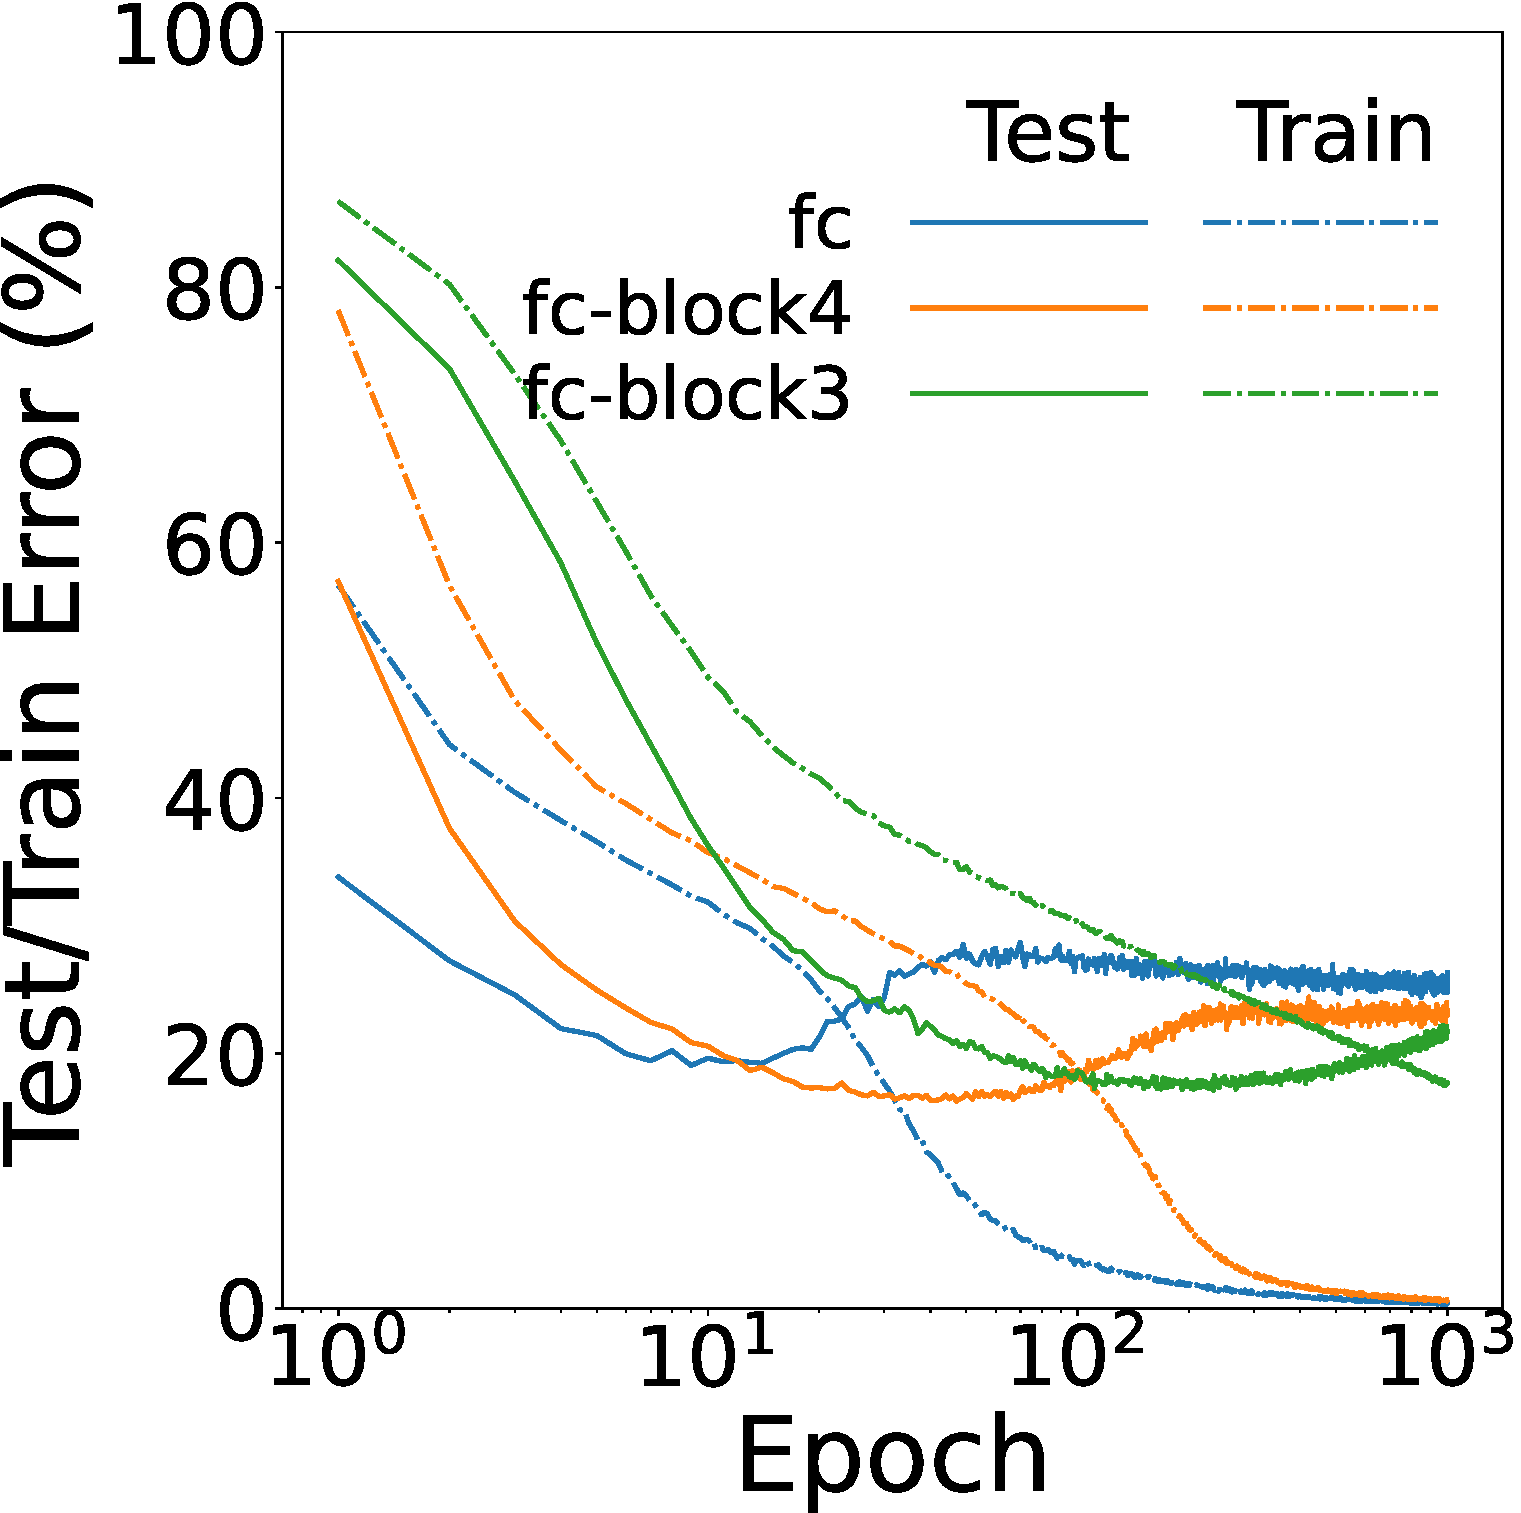
\includegraphics[keepaspectratio, width=0.45\linewidth]{fig/frozen_deep_layer_learning_curv.pdf} &
        \hspace{5pt} 
      %---- 2番目の図 --------------------------
      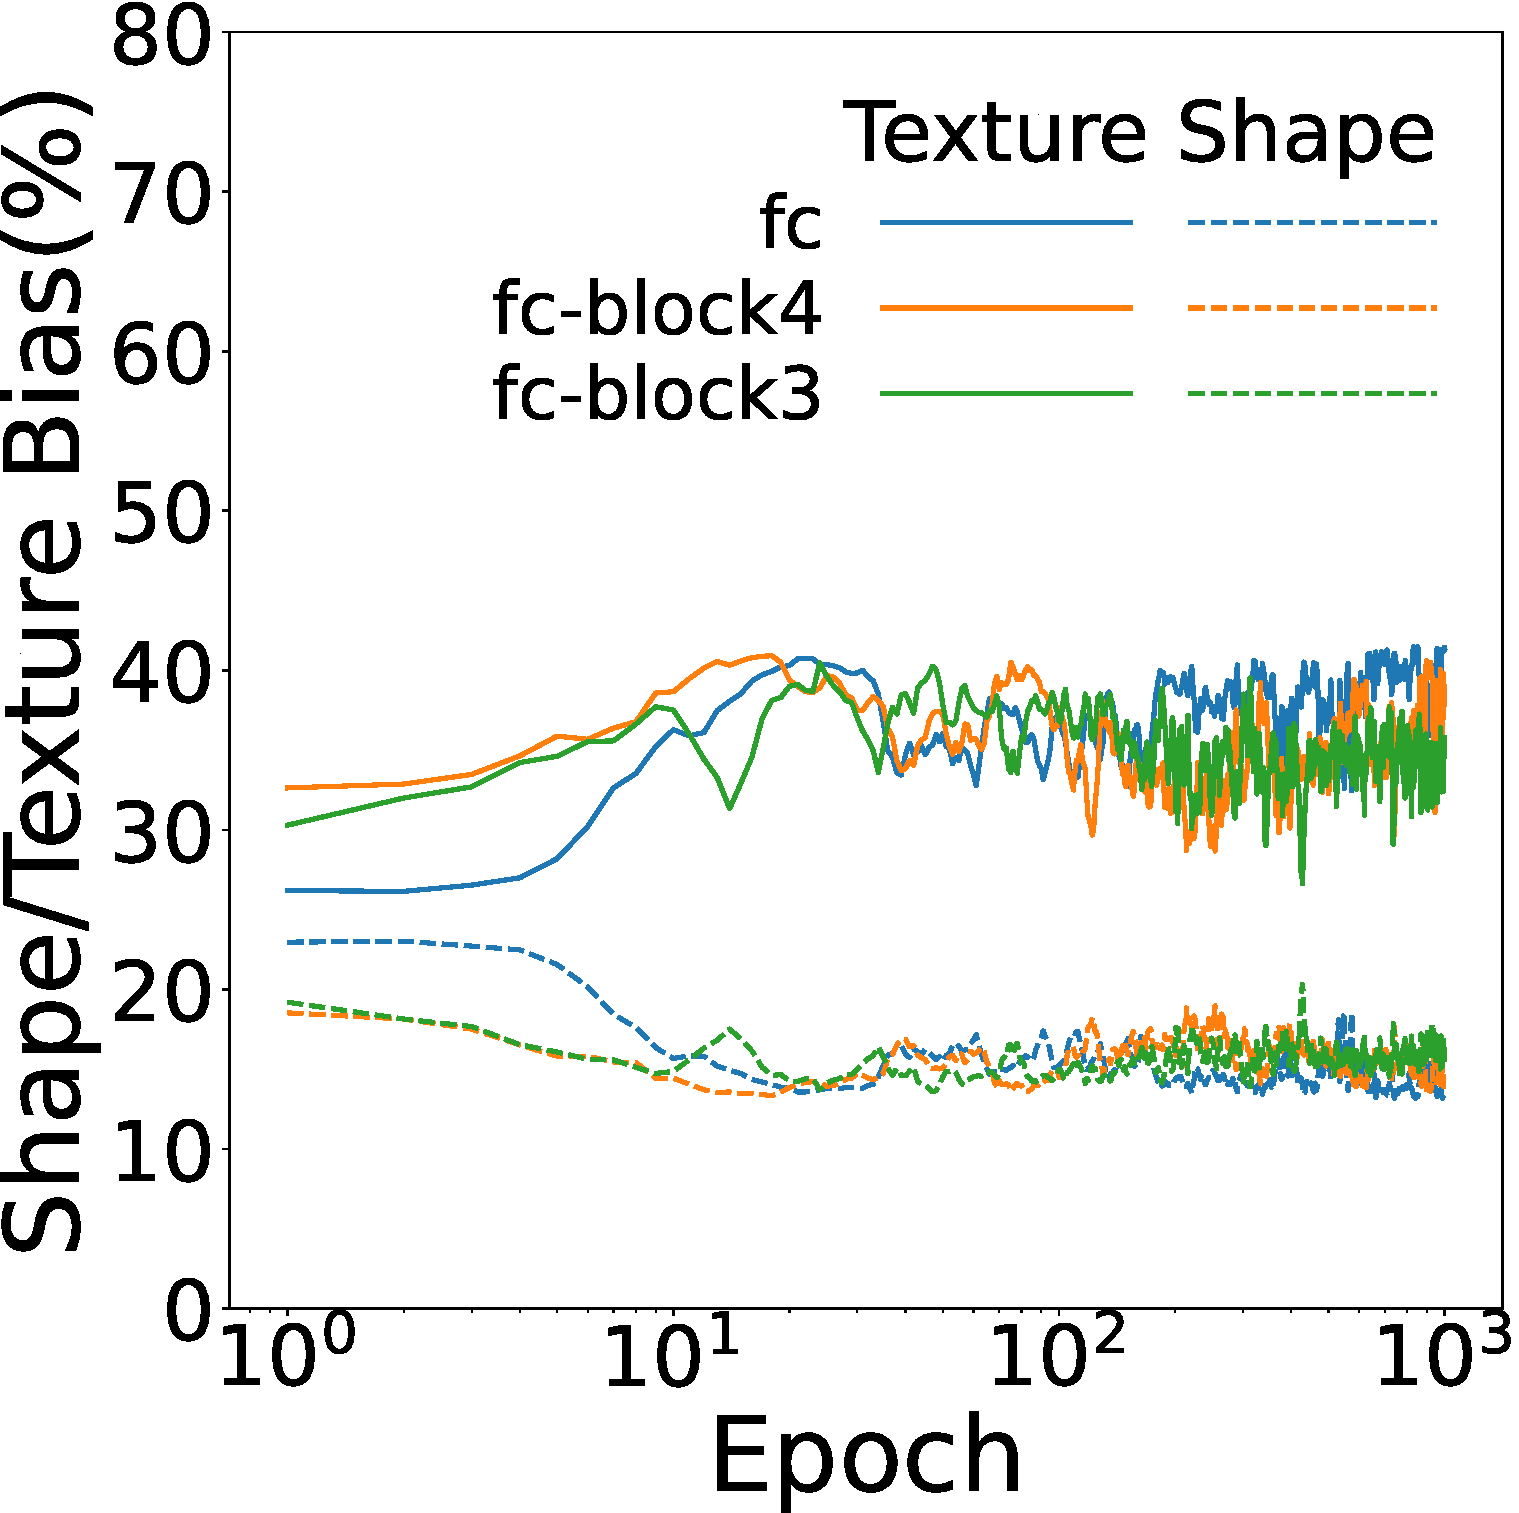
\includegraphics[keepaspectratio, width=0.45\linewidth]{fig/frozen_deep_layer_sha_tex.pdf}
   \end{tabular}
\caption[Learning processes under deep layer parameter freezes.]{Learning processes under deep layer parameter freezes. Left: train/test errors Right: shape/texture bias values.}
%Learning curve graphs for double descent and shape/texture bias for different label noise. \textbf{Left}:learning curve. \textbf{Right}:model's bias shift.}
\label{fig:comp_frozen_deep_layer}
\end{figure}

\begin{figure}[htb]
\centering
   \begin{tabular}{cc}
      %---- 最初の図 ---------------------------
      \hspace{-5mm}
      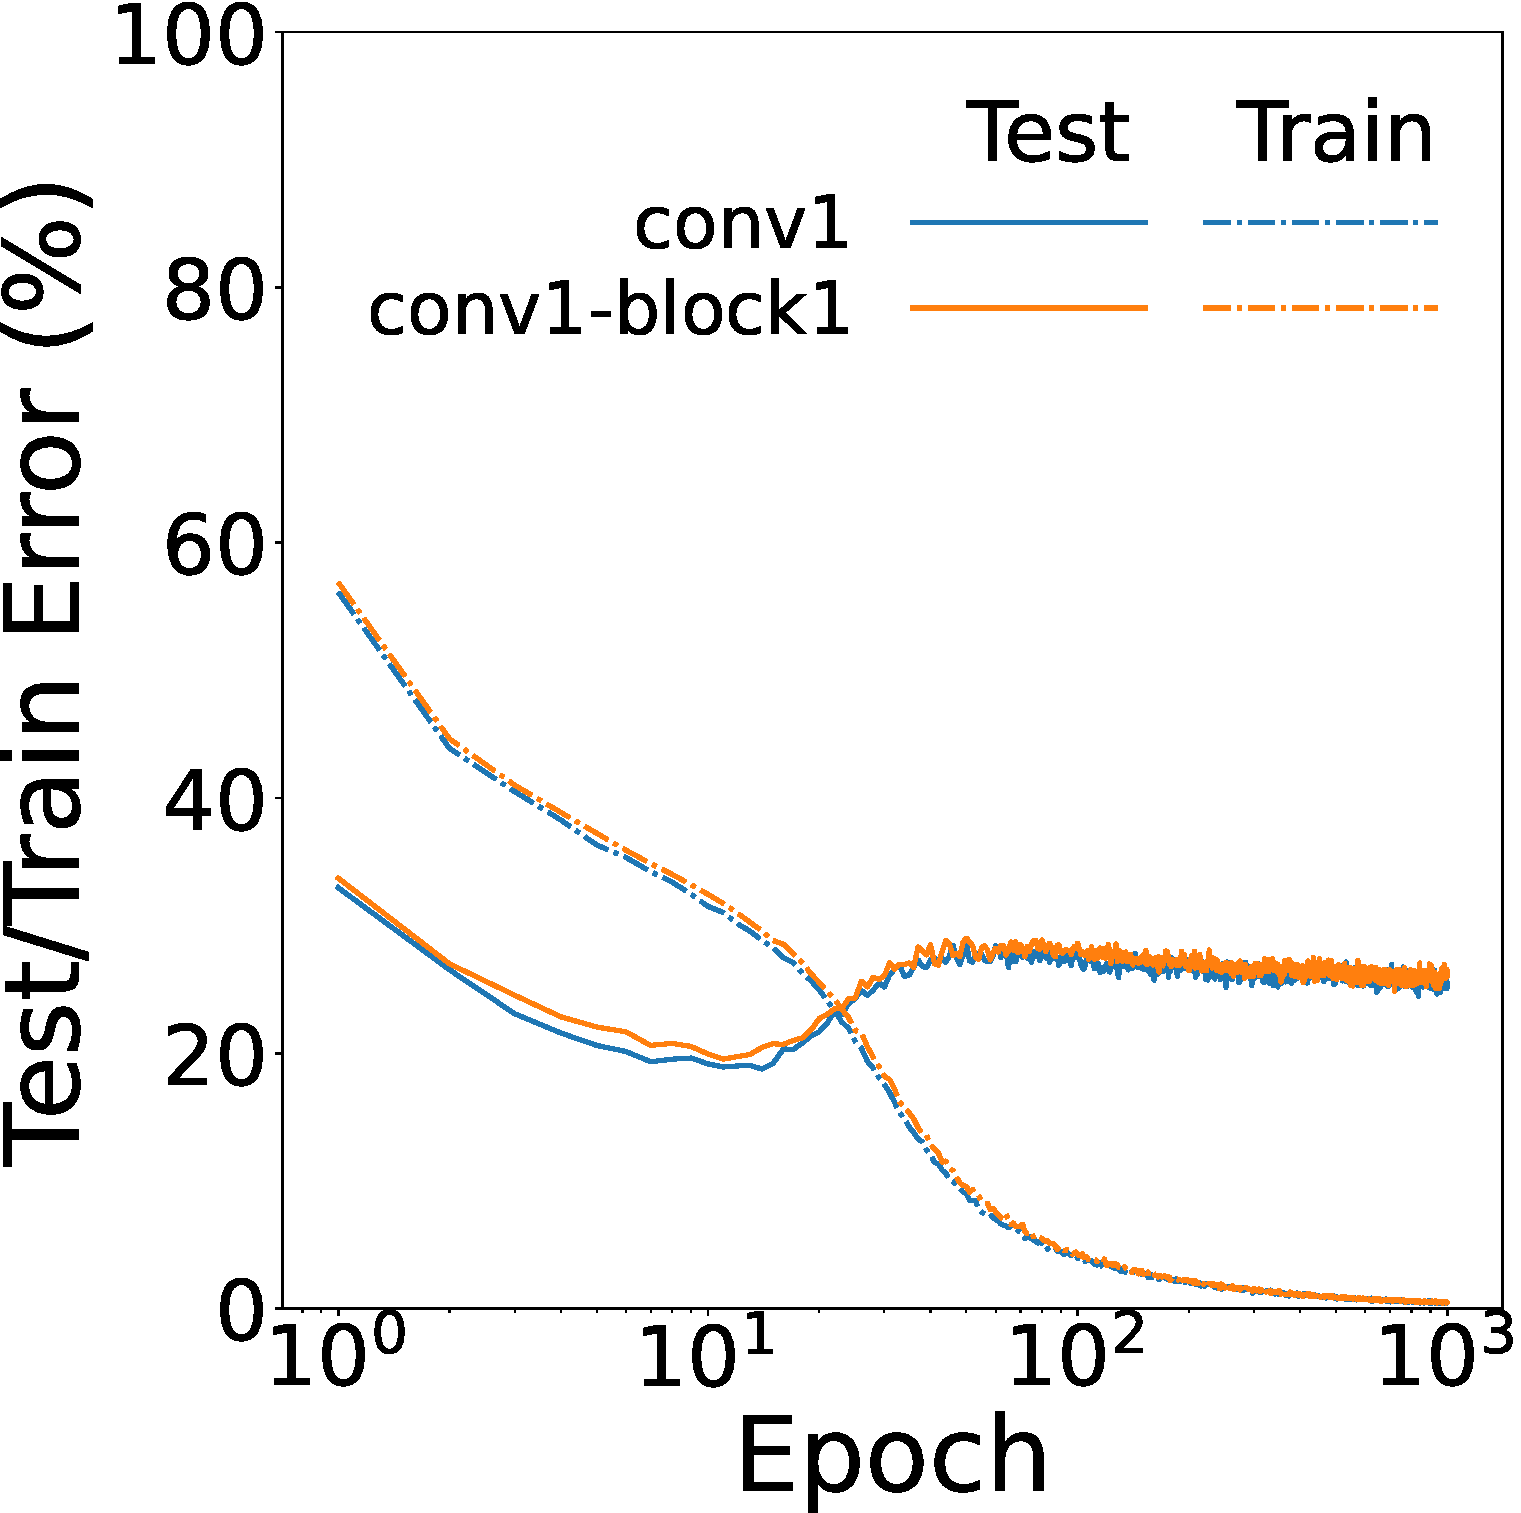
\includegraphics[keepaspectratio, width=0.45\linewidth]{fig/frozen_shallow_layer_learning_curv.pdf} &
        \hspace{5pt} 
      %---- 2番目の図 --------------------------
      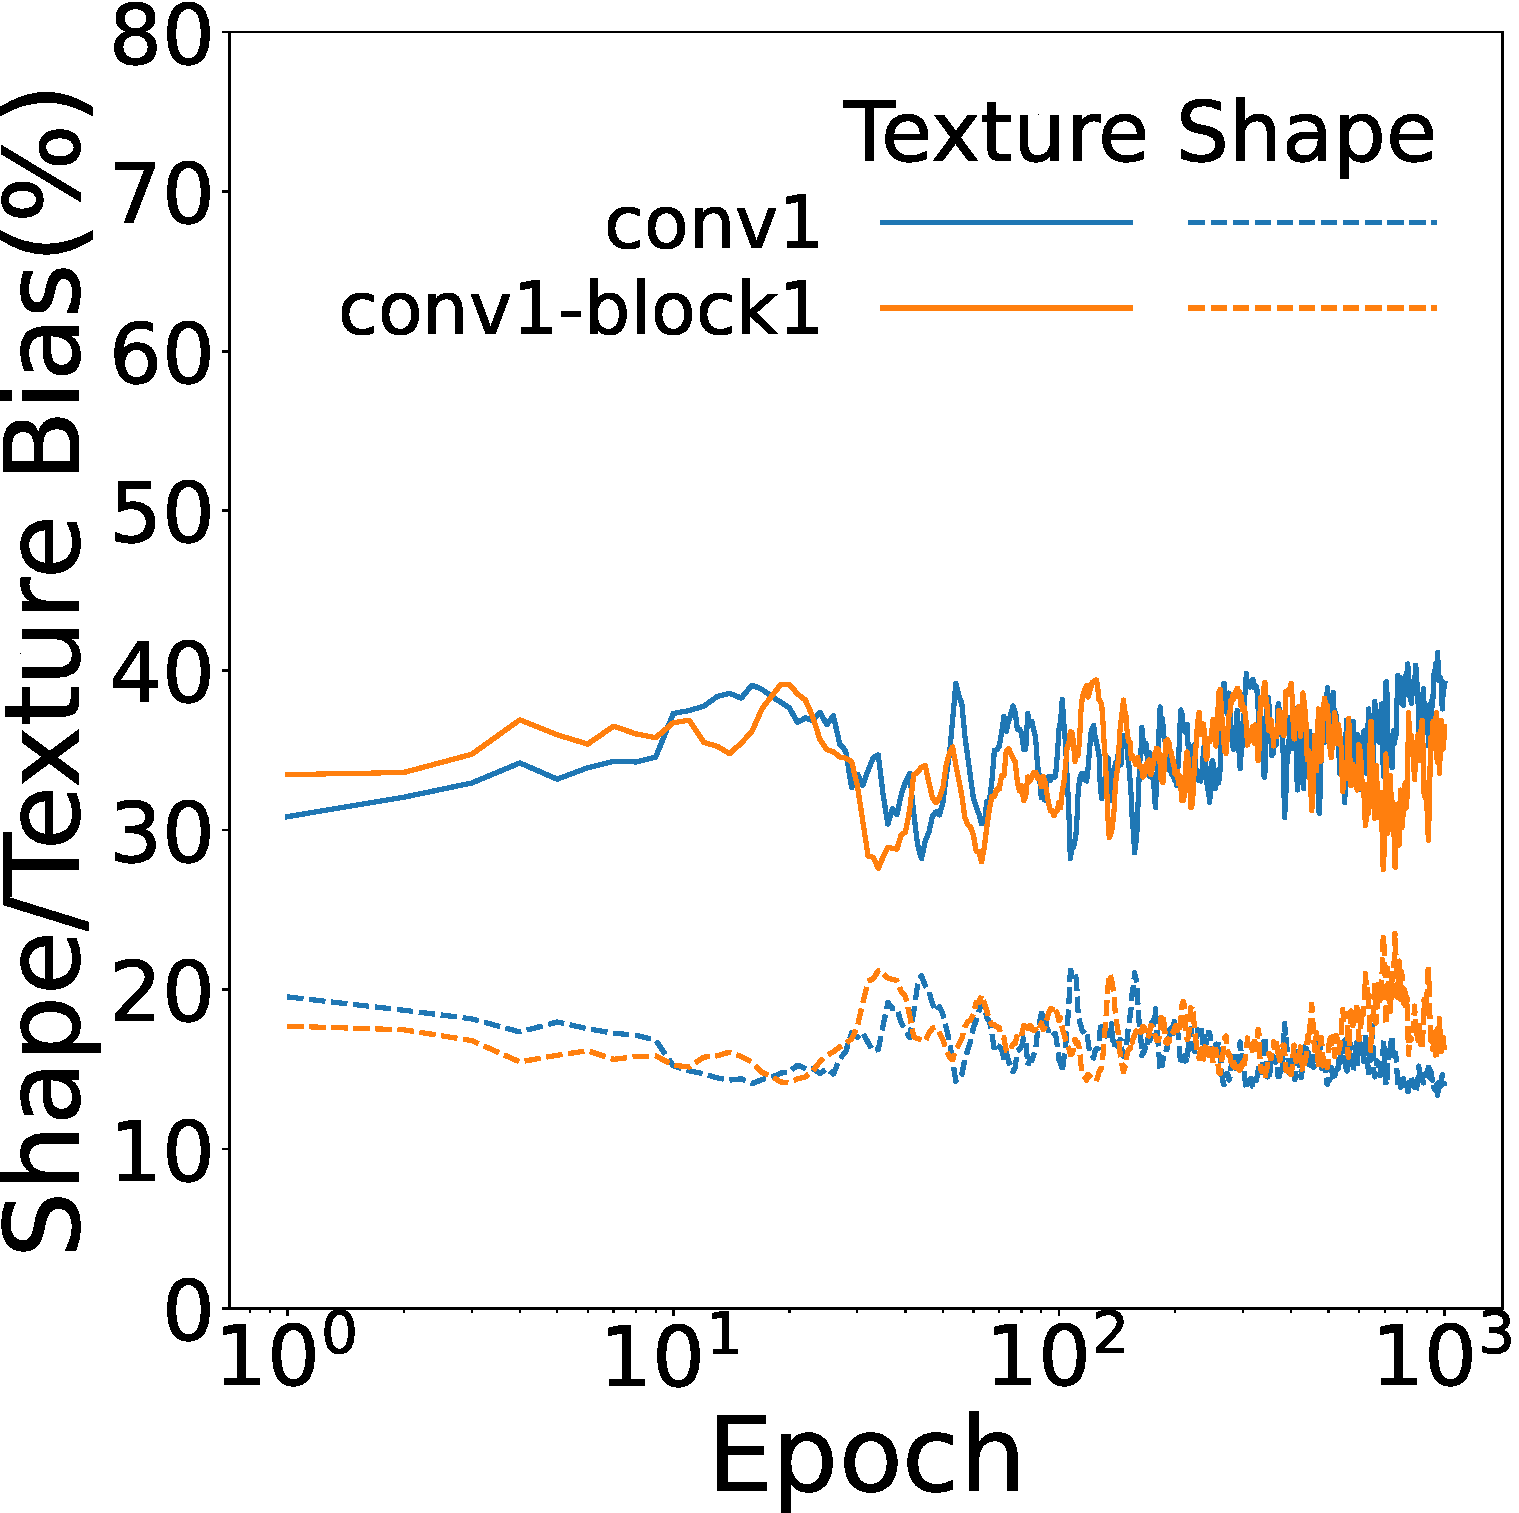
\includegraphics[keepaspectratio, width=0.45\linewidth]{fig/frozen_shallow_layer_sha_tex.pdf}
   \end{tabular}
\caption[Learning processes under shallow layer parameter freezes.]{Learning processes under shallow layer parameter freezes. Left: train/test errors Right: shape/texture bias values.}
%Learning curve graphs for double descent and shape/texture bias for different label noise. \textbf{Left}:learning curve. \textbf{Right}:model's bias shift.}
\label{fig:comp_frozen_shallow_layer}
\end{figure}
\newpage

% \chapter{考察}
本研究では,自然画像に存在する形状・テクスチャの特徴に着目し,二重下降現象との関係を分析した.その結果,ImageNetで事前学習を行った場合に,いくつかの条件において学習過程における二重降下とモデルが示す形状・テクスチャ偏重度の推移に相関がみられることがわかった.このような条件においては,二重降下における二度目の下降が始まるまでのテスト誤差と,形状・テクスチャ偏重度の推移との間に相関がみられる傾向にある.しかし,この相関は二度目の下降が始まると弱くなった.このような傾向は,二重降下を三つの段階に分割し,定性的,定量的に相関関係を評価することで判明した.

その後の実験では,CNNの最終畳み込み層で強く偏重度の独特なシフトが観察された.しかし,それ以前の中間層では,少なくとも検証を行った層においては,最終畳み込み層と同様の変化は見られなかった.この観察から,CNNの深い層は中間層とは異なる学習傾向を示す可能性が示唆される.

% 二重降下に関する先行研究では,データに存在する複数の特徴に影響されるのではないかという仮説が提唱されている.では,二重降下現象は形状やテクスチャーなどの特徴によって起こるのだろうか?我々はそうは考えていない.もし本当にそのような特徴によって現象が引き起こされるのであれば,二重降下の挙動と形状・テクスチャ偏重度は整理された傾向を示すはずである.例えば,まず形状偏重度がピークに達し,その後減少し,テクスチャ偏重度がピークに達する.しかし,実際には形状偏重度とテクスチャ偏重度それら自体が逆相関を見せている.また,事前学習を行わなかった場合には形状テクスチャ偏重度の特異な推移は見られなかった.したがって,double descentを引き起こす何らかの学習傾向によって,CNNの特徴抽出傾向が影響され,ImageNetで事前学習した場合において,double descentと偏重度の推移に相関を見せたと考える.(川勝先生の指摘あり,書き換え必須)
二重降下に関する先行研究では,データに存在する複数の特徴に影響されるのではないかという仮説が提唱されている.では,二重降下現象は形状やテクスチャーなどの特徴によって起こるのだろうか?我々は,その片鱗を観察したと考えている.今回の実験では,double descentを引き起こす何らかの学習傾向によって,CNNの特徴抽出傾向が影響され,ImageNetで事前学習した場合において,double descentと偏重度の推移に相関を見せたと考える.そのため,ImageNetで事前学習の有無で,パラメータの学習のされ方がどのように変わっているかを検証することは,二重降下を理解することにつながる可能性が考えられる.

実用的な観点からは,ImageNetを事前学習した条件下では,偏重度が最大,または最小となるepoch付近でテスト誤差が最大になる可能性が示唆され,この偏重度を観察することで,早期に停止できる最適,または準最適な学習エポック数を決定できる可能性が示唆される.さらに,二重降下を引き起こす要因が,特に深い層における形状やテクスチャの特徴に対するCNNの偏重度合いにも影響を与える可能性があることを示した.

本研究では,CNNが形状やテクスチャといった画像特徴をどのように学習していくかに着目し,複数の条件において二重降下との関係を検証した.深層学習において,未解明なことは多数存在し,double descentもその一つである.そのような中で,特に深層に目を向けるべきであるとした本研究は,今後の研究の一つの方向性を指示したと考える.しかし,今回見られた現象の具体的なメカニズムを示せていないことは一つの限界点である.
本研究では,CNNによる形状やテクスチャといった画像特徴の学習過程に注目し,さまざまな条件下における二重降下現象との関連性を検証した.深層学習における未解明の領域は多数存在し,二重降下現象はその一つである.本研究は,特に深層学習の深い層への理解を深めることの重要性を指摘し,将来の研究に対する一つの有望な方向性を提供するものと考えられる.しかしながら,観測された現象の具体的な機構に関しては明確な説明を提供できていない.この点は,今後の研究における主要な課題である.
\newpage

% \chapter{結論}
本稿では,epoch-wise double descentの先行研究に触発され,まだ理論的な解析がなされていない画像固有の特徴(形状・テクスチャ)と二重降下の関係に着目した.まず,画像特徴の獲得過程を追跡するため,既存の手法を用いて形状・テクスチャに対するモデルの偏重度を定量化し,この偏重度と学習中のテスト誤差の推移を比較した.結果として,ImageNetを事前学習した場合に,いくつかの条件下では,学習過程における形状・テクスチャ偏重度の推移とテスト誤り率が描くepoch-wise double descentの推移に相関がみられることがわかった.また,定量的な評価を通して,テスト誤り率の一度目の下降から上昇しきるまでの区間において特に相関が確認された.

さらに,定性的な可視化により,初期層におけるフィルタ,レイヤーの深さに基づく形状・テクスチャ偏重度の変化を示した.より深い層においては形状・テクスチャ偏重度に変化を示すが,初期層のフィルターはほとんど変化しないことが観察された.このような結果から,double descentの観点においては,深い層に着目するべきであると考えられる.我々の研究は,epoch-wise double descentと,深層学習と二重降下の一般的な分野の両方について,より広い理解に貢献すると考える.
\newpage

% % \chapter{今後の展望}
% \newpage

% \addcontentsline{toc}{chapter}{謝辞}
\chapter*{謝辞}
本修士論文は,東京電機大学システムデザイン工学研究科データ科学・機械学習研究室に所属し,前田英作教授の指導の下で執筆を行いました.3年半の間,研究指導にとどまらず,人生の道標となるような教えを賜りました指導教員の前田英作教授に厚く感謝申し上げます.
修士1年の1年間,副指導教員の前田 高志ニコラス准教授にはCTGの異常検知研究において,研究の方向性について貴重なご助言をいただきました.深く感謝申し上げます.
修士2年の1年間,本研究の遂行にあたり、副指導教員の川勝真喜准教授には修士2年次を通じて的確なご指導を賜りました。先生との議論を通じて既存の枠組みにとらわれない思考が培われ、研究の深化に大きく貢献していただきました。心より感謝申し上げます。

研究テーマの変更の上で,初期に有益な助言をいただき,その後の自身の研究において多大な貢献をしていただいたアルムナイの\UTF{9AD9}橋 秀弥氏に厚く感謝申し上げます.
研究室の前任事務岩本陽子氏,現任事務佐々木理央氏には,学会参加等の事務手続きにおいて多くの助力を賜り,修士生活を支えていただきました.深く感謝申し上げます.

酒造正樹客員教授には,論文指導等,研究生活において多くの助力を賜りました.厚く感謝申しあげます.

研究活動における数回の論文提出に際して,多くの助力をいただいた後輩の平本麗弥氏,小林慧音氏に深く感謝申し上げます.
研究生活において,議論,相談に付き合っていただいたり,疑問に答えていただいたデータ科学機械学習研究室の先輩,同期,後輩の皆様にも感謝を申し上げます.
産業技術総合研究所上級主任研究員片岡裕雄氏,東京工業大学横田理央教授,井上中順准教授,株式会社天地人 中村凌氏には,国際学会提出の際に,実験,執筆の双方に多くの助言と助力を賜りました.厚く御礼申し上げます.

最後に,私の生活を支えてくださった家族・友人に最大の感謝を申し上げます.

\newpage


% \renewcommand{\bibname}{参考文献}
\addcontentsline{toc}{chapter}{参考文献}  
% \begin{thebibliography}{99}
% \bibitem{sample}
% sample

% \end{thebibliography}
\bibliographystyle{ref/ieee_fullname.bst}
% \bibliographystyle{alpha}
\bibliography{ref/mybibfile}

% \appendix
% \chapter{付録}
\label{付録}

\section{EMNIST Digitsデータセットの基礎データ}
\begin{figure}[H]
    \centering
    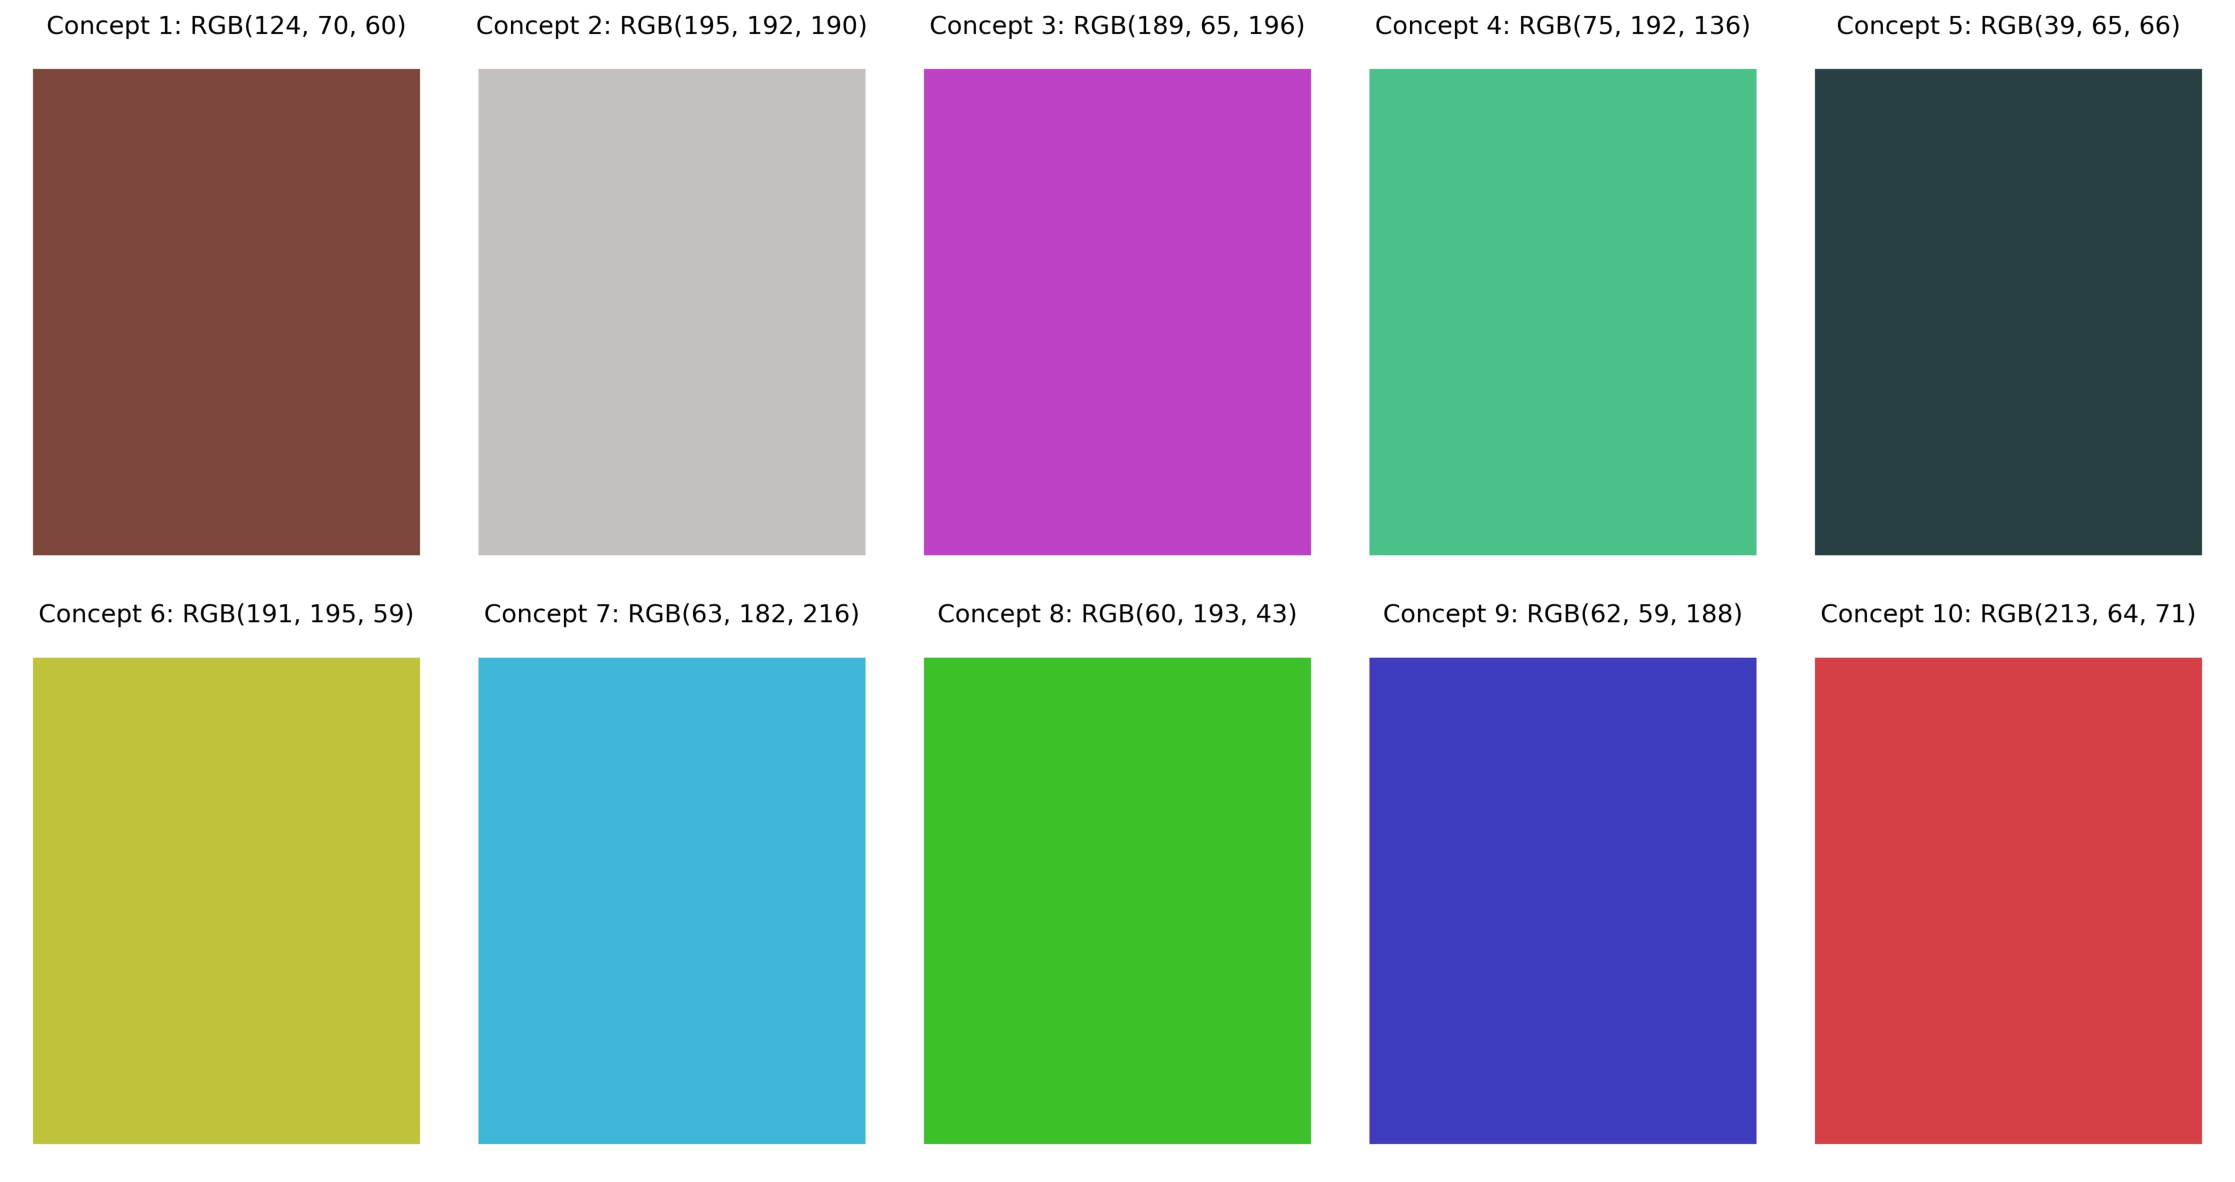
\includegraphics[width=\linewidth]{fig/color_varinace/0.pdf}
    \caption{$\sigma^2 = 0.0$の場合の各色クラスの色の例}
    \label{fig:variance_0}
\end{figure}

\begin{figure}[H]
    \centering
    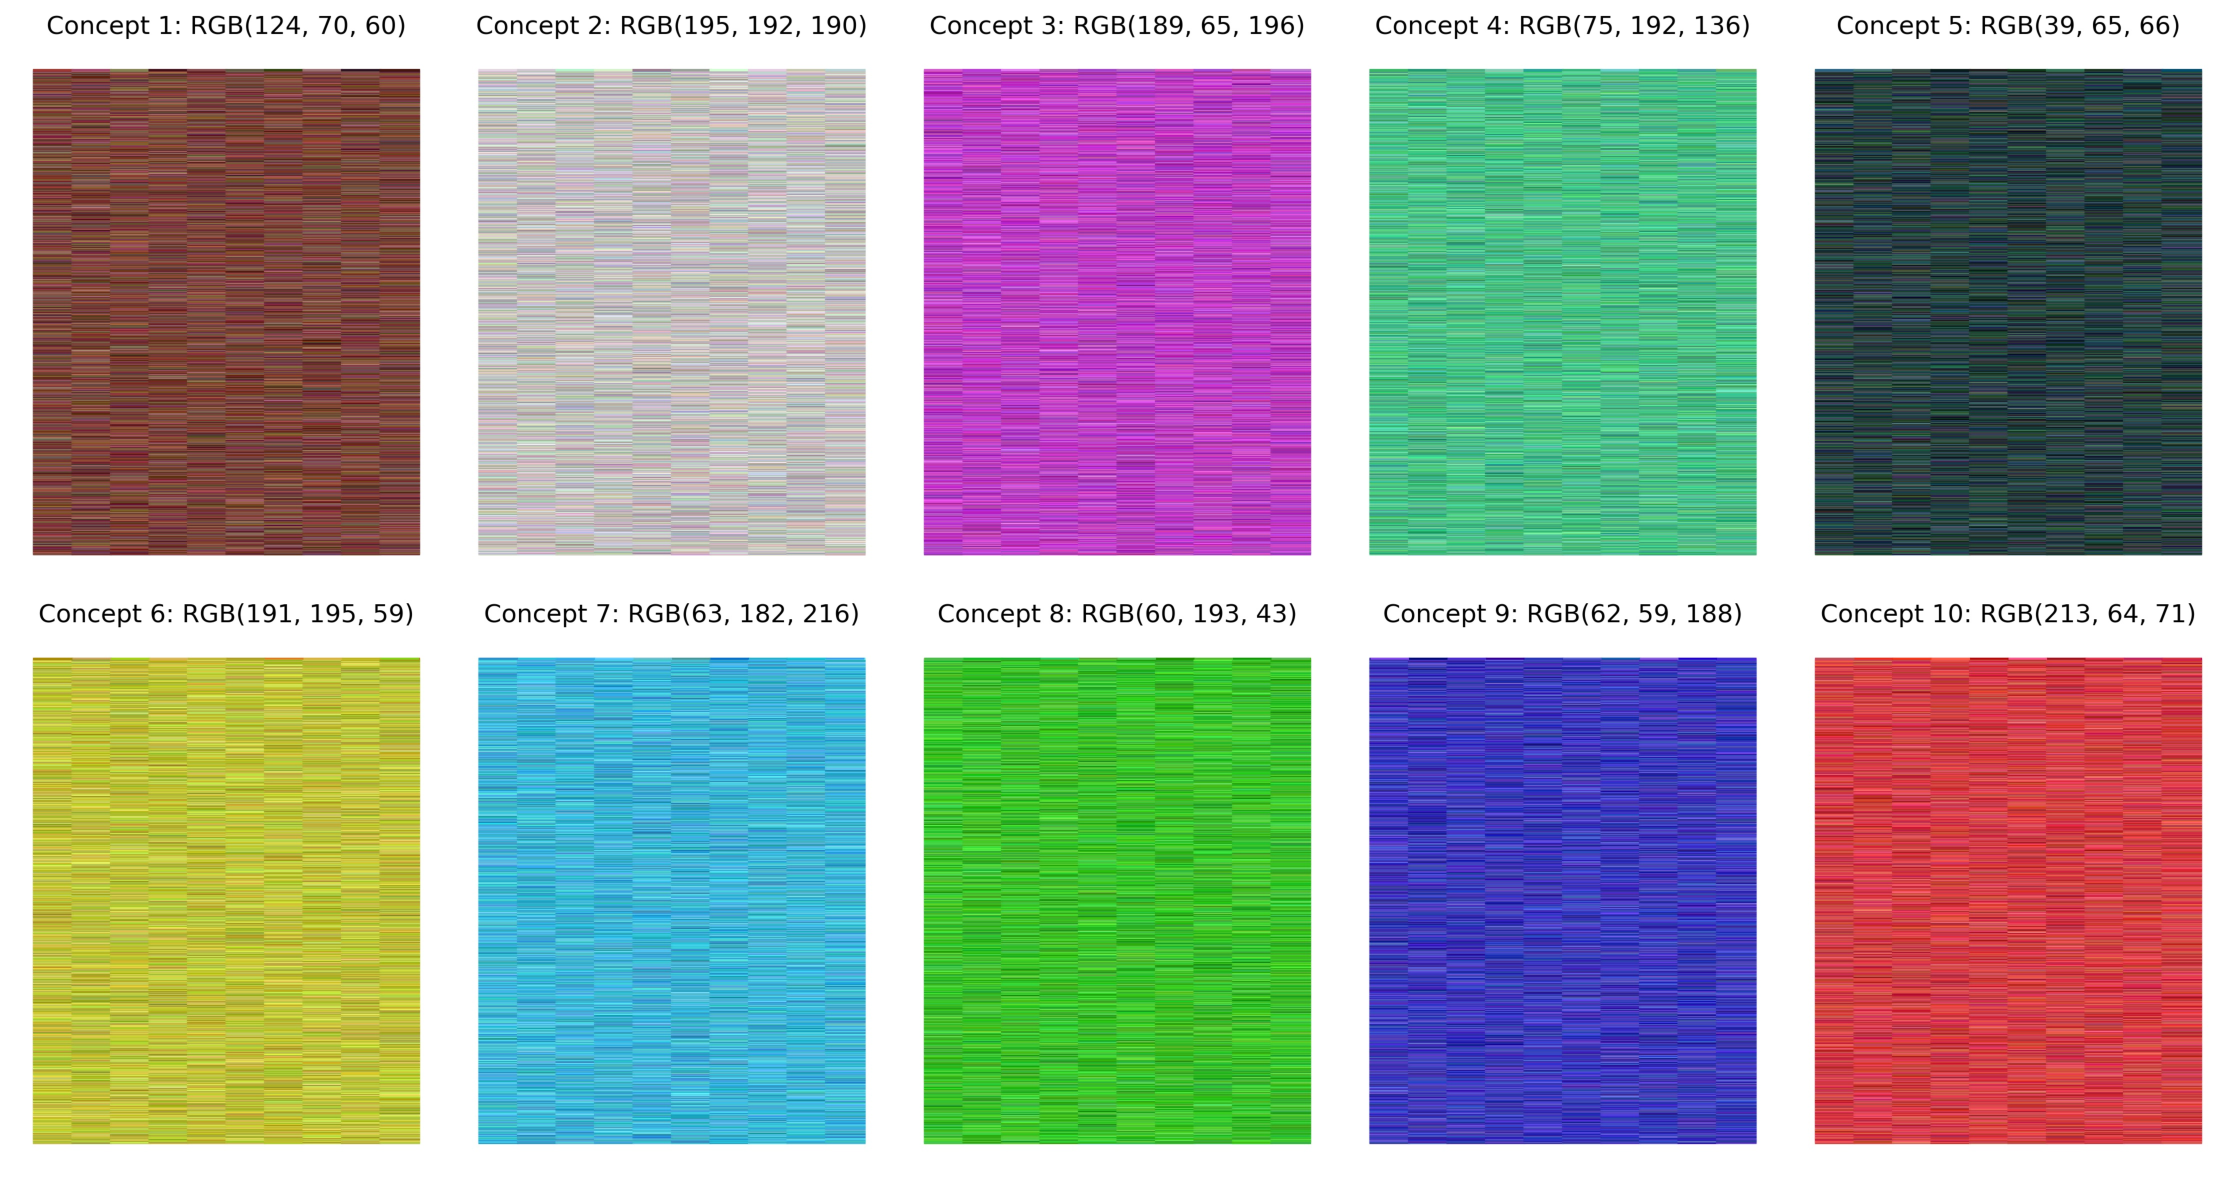
\includegraphics[width=\linewidth]{fig/color_varinace/1000.pdf}
    \caption{$\sigma^2 = 10^3$の場合の各色クラスの色の例}
    \label{fig:variance_1000}
\end{figure}

\begin{figure}[H]
    \centering
    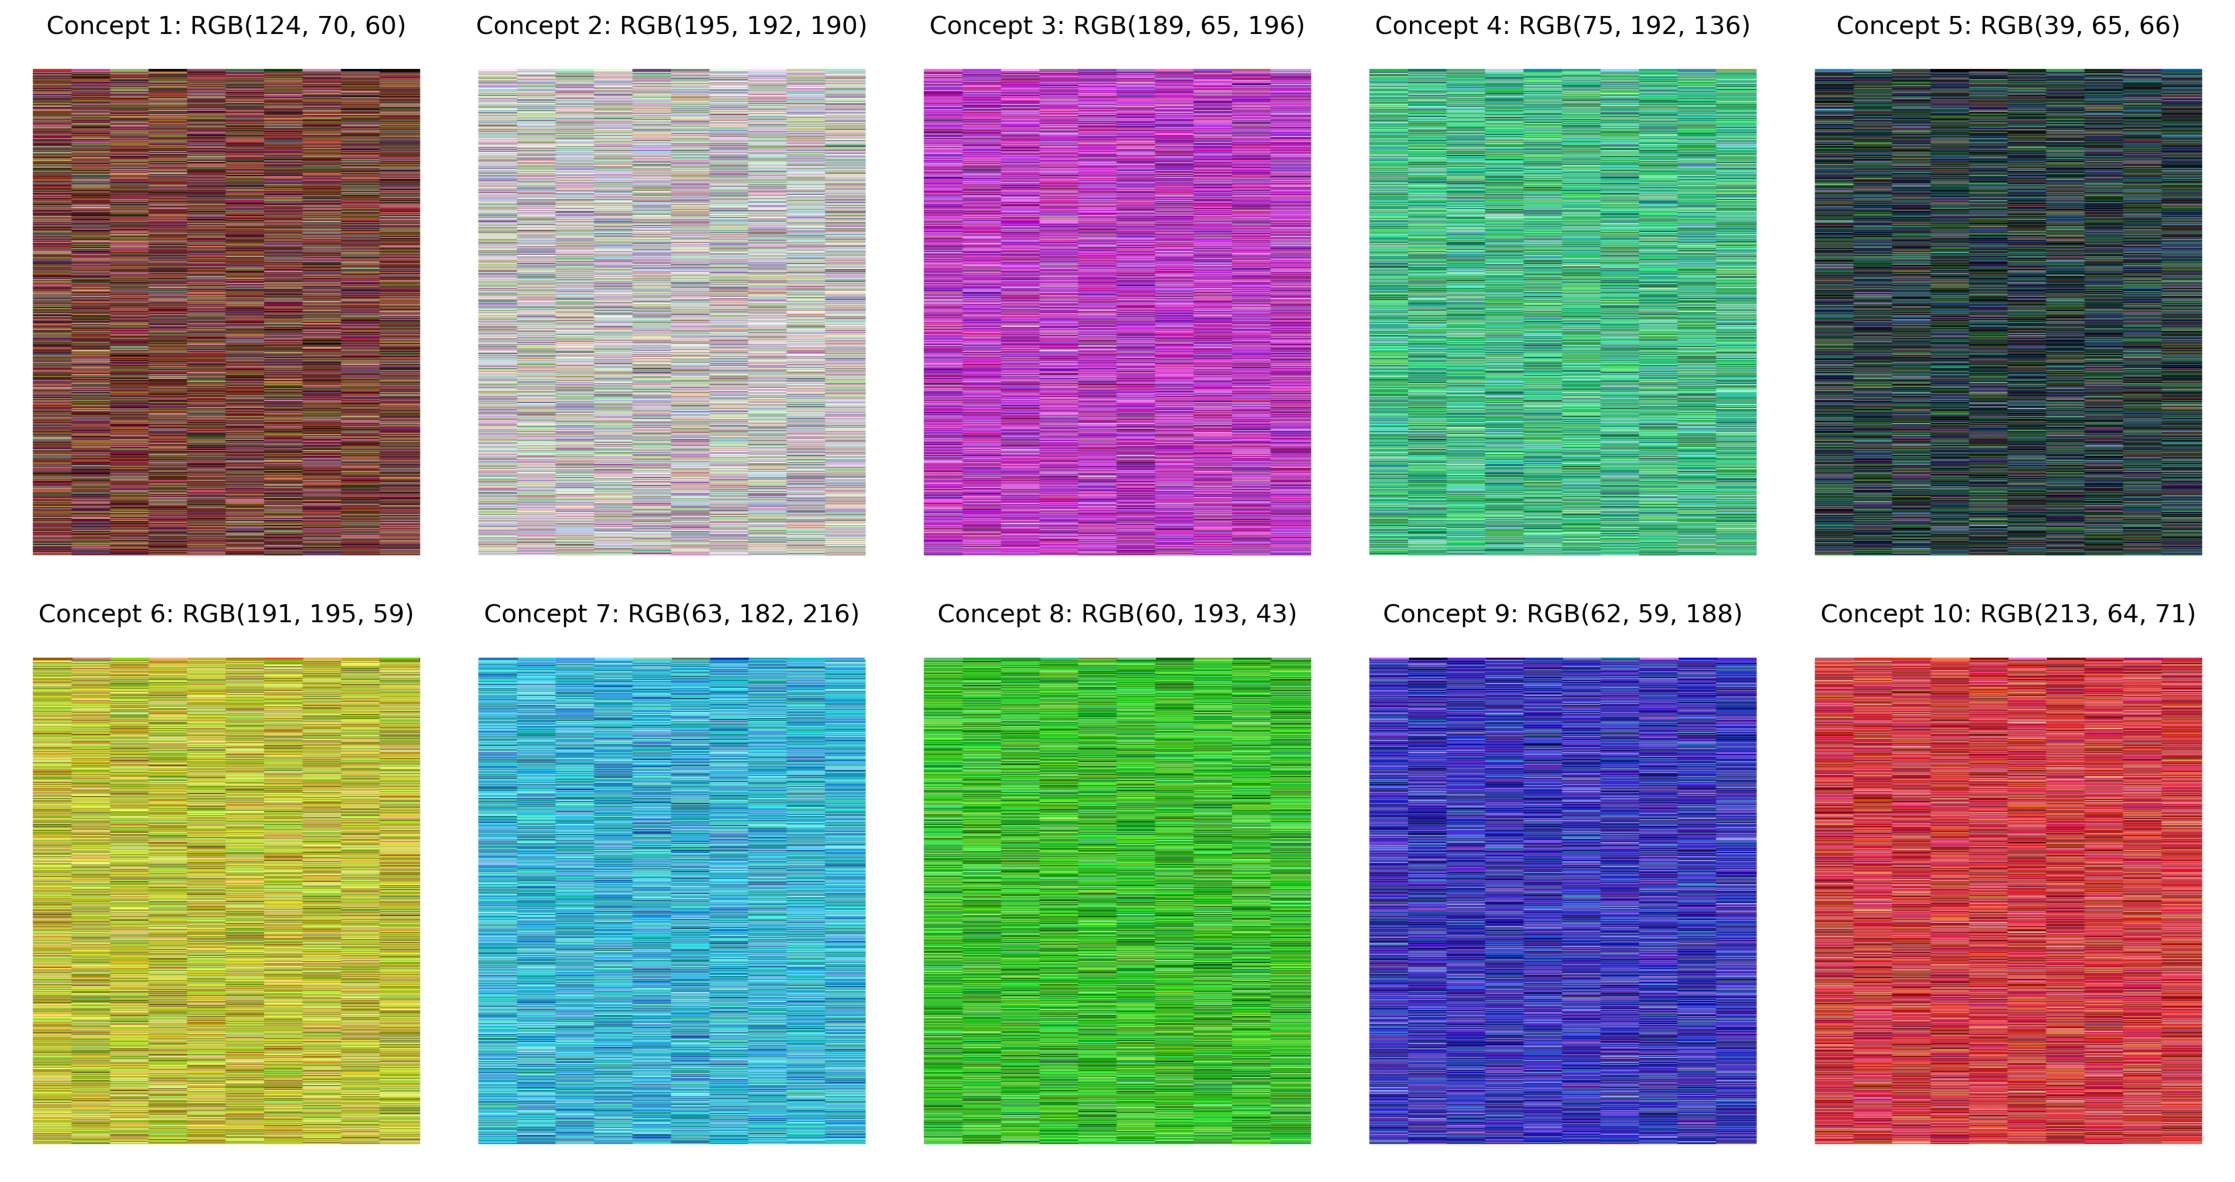
\includegraphics[width=\linewidth]{fig/color_varinace/3612.pdf}
    \caption{$\sigma^2 = 10^{3.5}$の場合の各色クラスの色の例}
    \label{fig:variance_3612}
\end{figure}

\begin{figure}[H]
    \centering
    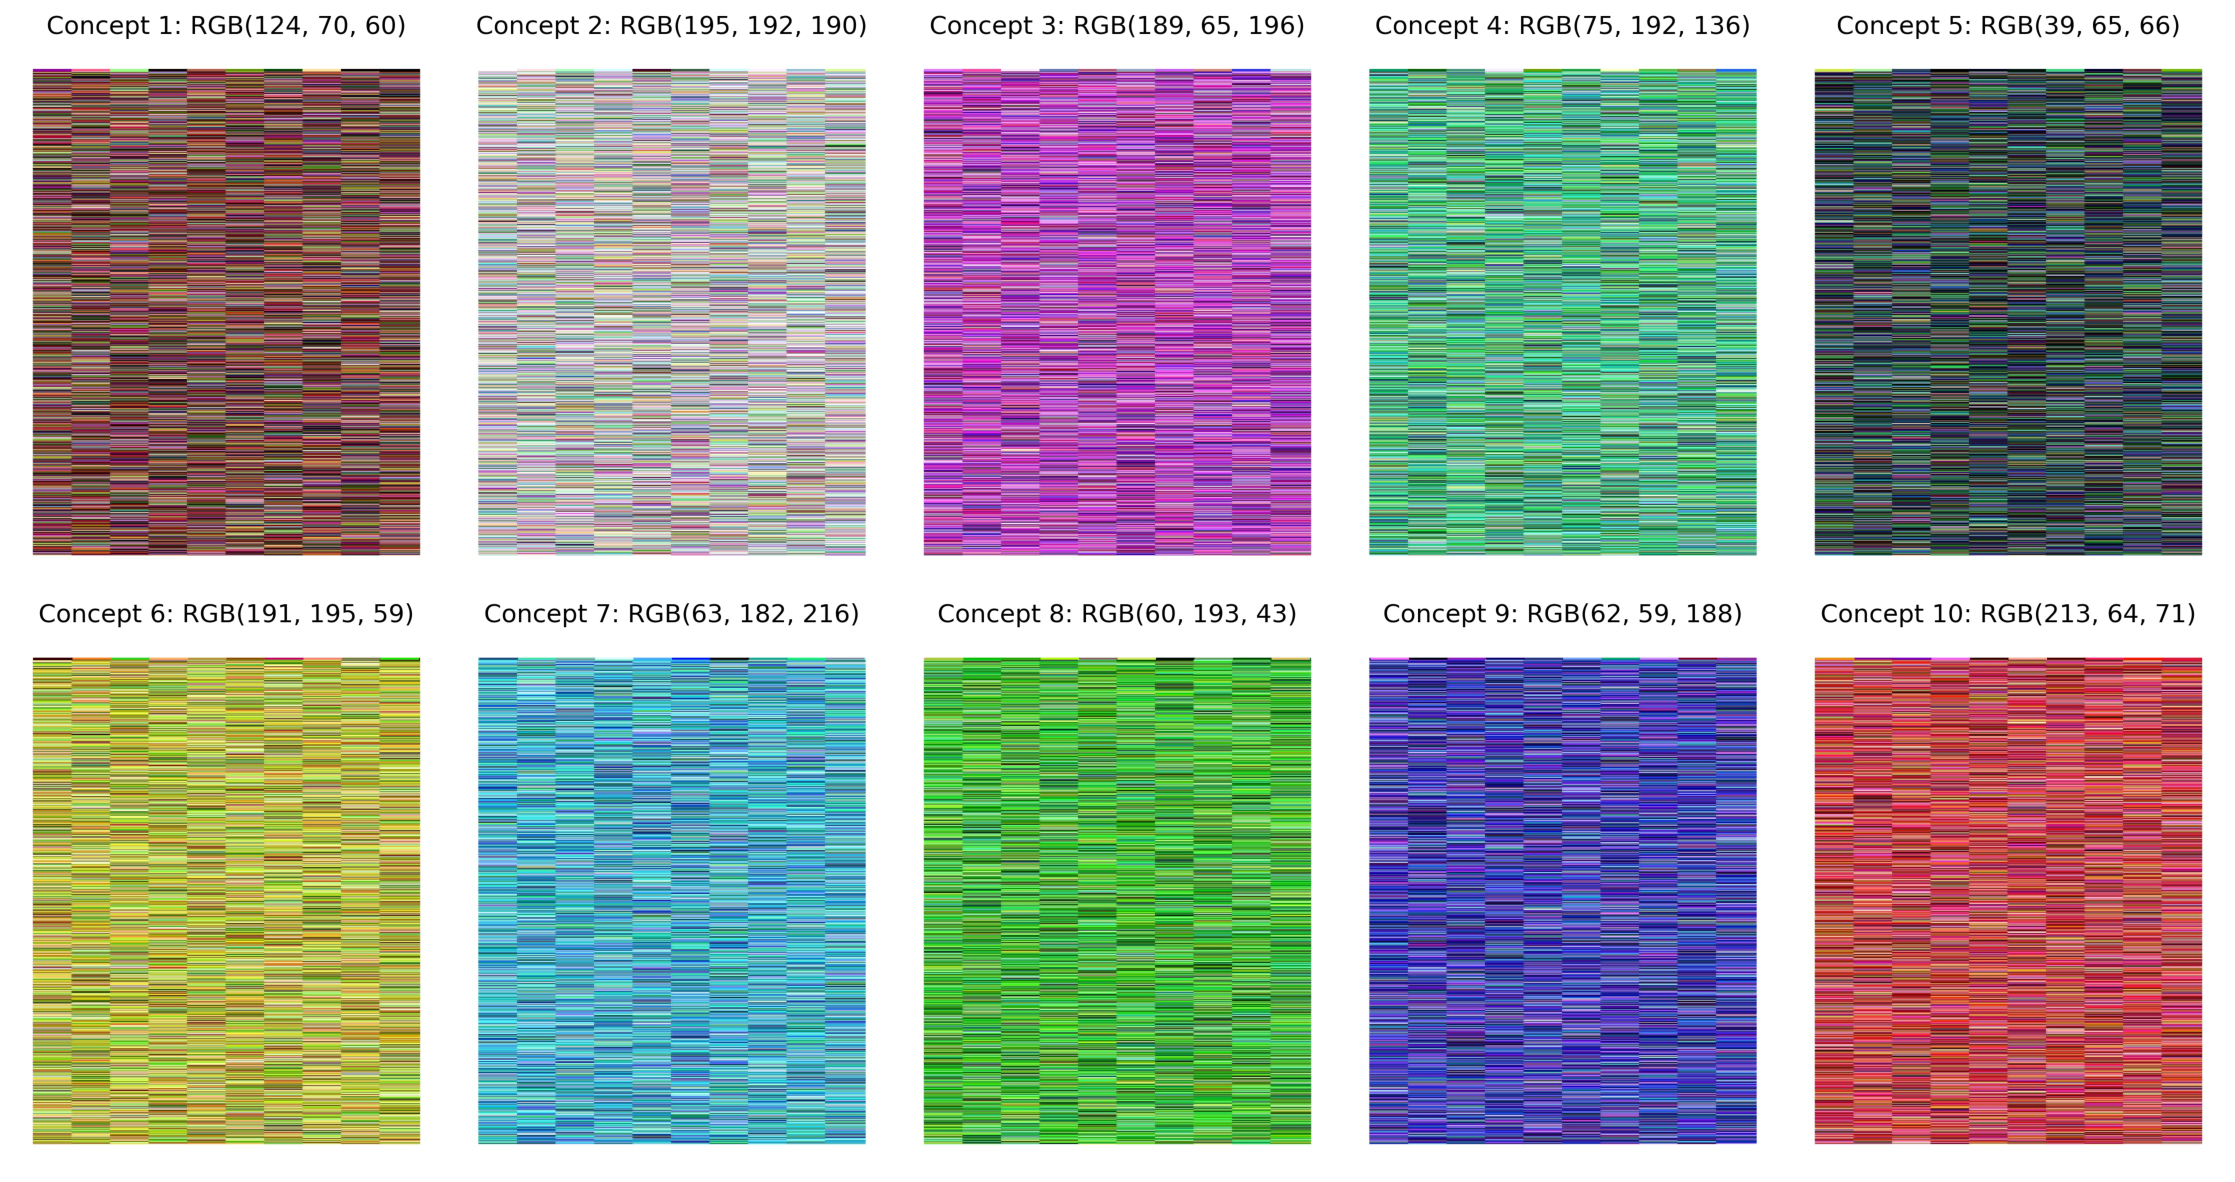
\includegraphics[width=\linewidth]{fig/color_varinace/10000.pdf}
    \caption{$\sigma^2 = 10^4$の場合の各色クラスの色の例}
    \label{fig:variance_10000}
\end{figure}

\begin{figure}[H]
    \centering
    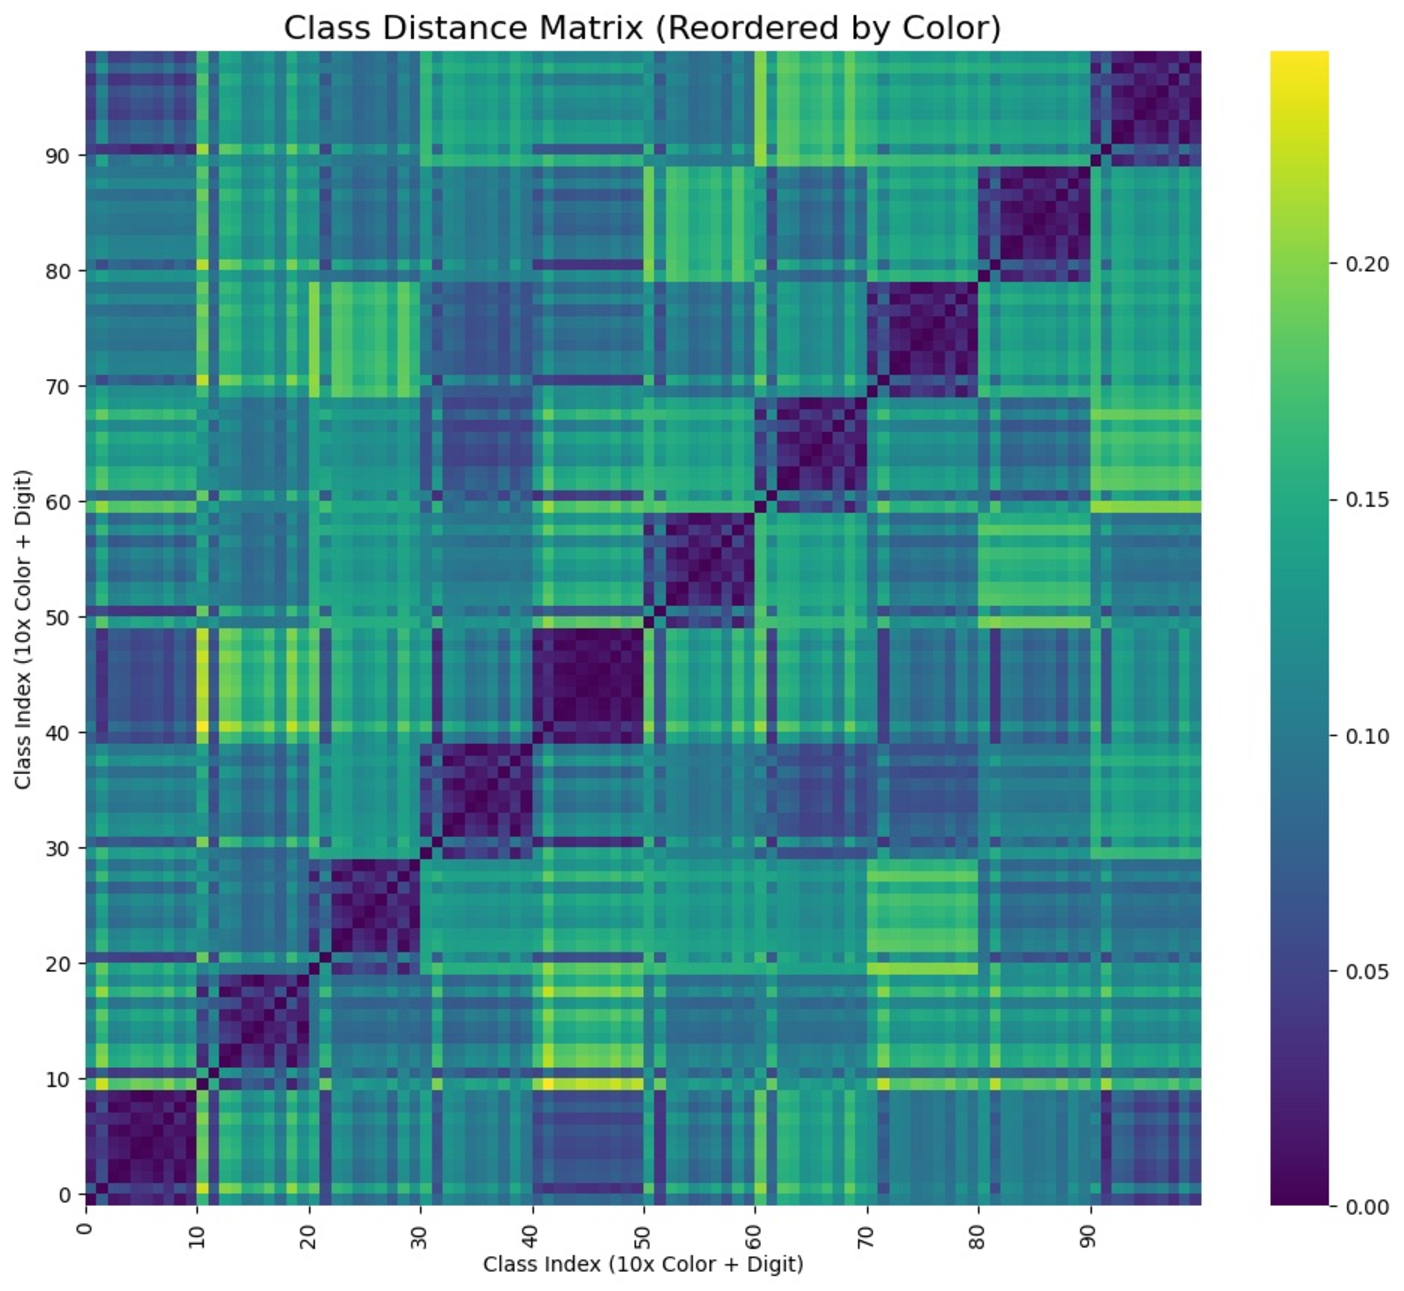
\includegraphics[width=\linewidth]{fig/distance_matrix_heatmap_by_color.pdf}
    \caption{100クラスのクラス間距離のヒートマップ(色,数字順)}
    \label{fig:distance_matrix_heatmap_by_color}
\end{figure}

\begin{figure}[H]
    \centering
    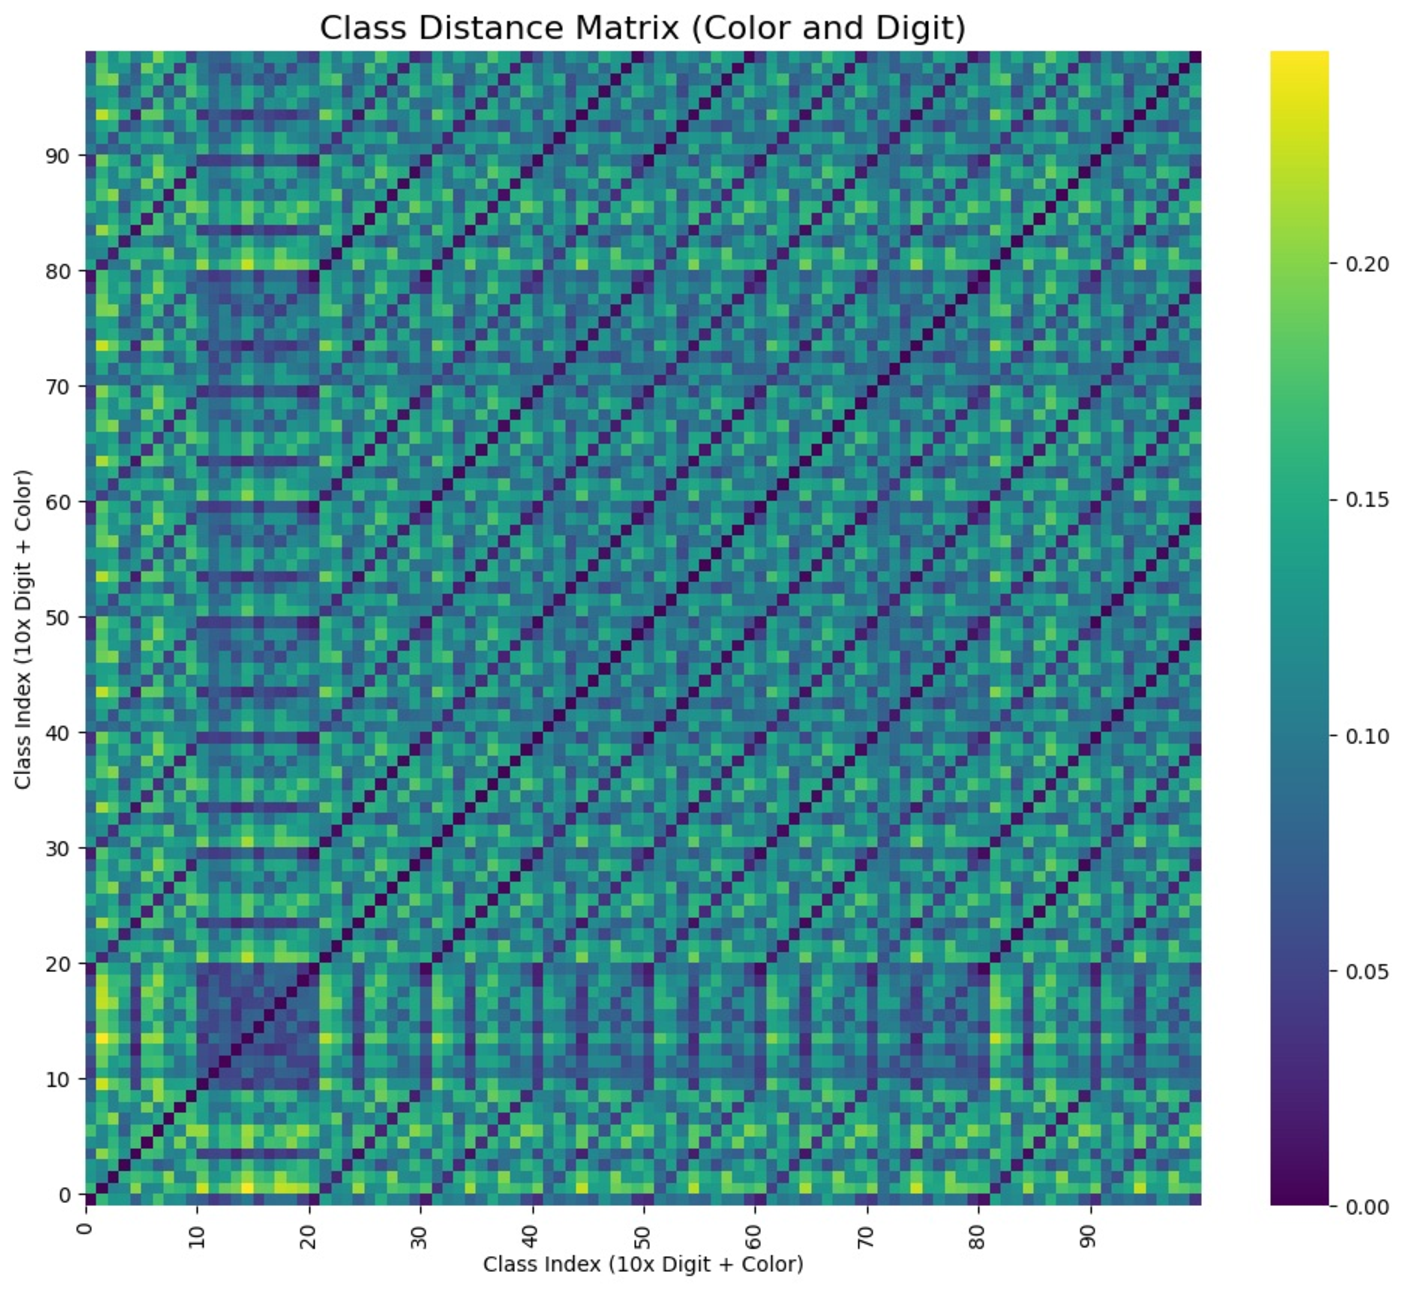
\includegraphics[width=\linewidth]{fig/distance_matrix_heatmap.pdf}
    \caption{100クラスのクラス間距離のヒートマップ(数字,色順)}
    \label{fig:distance_matrix_heatmap_by_digit}
\end{figure}



% % \chapter*{付録}
% \addcontentsline{toc}{chapter}{付録}
\chapter{学習プログラム}
\label{学習プログラム}
学習に利用したプログラムを示す.掲載したプログラムは,GitHub上で公開している.
\\
\url{https://github.com/dsml-lab/double_descent_and_shape_texture_bias}
% カスタムスタイルの定義
\lstdefinestyle{pythonstyle}{
    language=Python,
    basicstyle=\ttfamily\small,
    keywordstyle=\color{blue},
    stringstyle=\color{orange},
    commentstyle=\color{gray}\itshape,
    numbers=left,
    numberstyle=\tiny\color{gray},
    stepnumber=1,
    numbersep=5pt,
    backgroundcolor=\color{lightgray!10},
    frame=single,
    breaklines=true,
    showstringspaces=false,
    captionpos=b
}

\begin{lstlisting}[style=pythonstyle, caption={メインコード}]
    # combineのラベルノイズに関して、色・数字のラベル両方異なるラベルにする
    # accuracyに関して、combineの正解率だけでなく、色・数字の正解率も出力する
    # ラベルノイズの正解率とラベルノイズでない正解率を出力する
    # 平均・分散も出力する
    # 重みの加え方が均等
    
    import os
    import torch
    import torch.nn as nn
    import torch.optim as optim
    import torch.nn.functional as f
    import torch.backends.cudnn as cudnn
    from torch.cuda.amp import autocast, GradScaler
    from torch.utils.data.sampler import Sampler
    import torchvision.transforms as transforms
    from torch.utils.data import DataLoader, TensorDataset
    from sklearn.metrics import classification_report
    from sklearn.metrics import accuracy_score
    import math
    import torchvision.models as models
    import numpy as np
    import time
    import wandb
    import argparse
    import random
    import matplotlib.pyplot as plt
    import csv 
    import warnings
    import gc
    import gzip
    # import models written by scratch
    from model.cnn_2layers import CNN2Layer
    from model.cnn_3layers import CNN3Layer
    from model.cnn_4layers import CNN4Layer
    from model.cnn_5layers import CNN5Layer
    from model.cnn_8layers import CNN8Layer
    from model.cnn_16layers import CNN16Layer
    from model.resnet18 import ResNet18
    # download datasets from pytorch
    from torchvision import datasets
    
    # Ignore warnings
    warnings.filterwarnings("ignore")
    # os.environ['CUDA_LAUNCH_BLOCKING'] = "1"
    # os.environ['PYTORCH_CUDA_ALLOC_CONF'] = 'max_split_size_mb:128'
    torch.backends.cudnn.benchmark = True
    
    # settings
    def parse_args():
        """
        Parse the command-line arguments.
        
        Returns:
            argparse.Namespace: The parsed command-line arguments.
        """
        arg_parser = argparse.ArgumentParser()
        #set seed
        arg_parser.add_argument("-seed", "--fix_seed", type=int, default=42)
        
        #set model settings
        arg_parser.add_argument("--model", type=str, choices=["cnn_2layers", "cnn_3layers", "cnn_4layers", "cnn_5layers", "cnn_8layers", "cnn_16layers", "resnet18"], help="モデルアーキテクチャの選択")
        arg_parser.add_argument("-model_width", "--model_width", type=int, default=1)
        arg_parser.add_argument("-epoch", "--epoch", type=int, default=1000)
        
        #set dataset setting
        arg_parser.add_argument("-datasets", "--dataset", type=str, choices=["mnist", "emnist", "emnist_digits", "cifar10", "cifar100", "tinyImageNet", "colored_emnist", "distribution_colored_emnist"], default="cifar10")
        arg_parser.add_argument("-variance", "--variance", type=int, default=10000)
        arg_parser.add_argument("-correlation", "--correlation", type=float, default=0.5)
        arg_parser.add_argument("-label_noise_rate", "--label_noise_rate", type=float, default=0.0) 
        arg_parser.add_argument("-gray_scale", "--gray_scale", action='store_true', help="グレースケールに変換するかどうか")
        arg_parser.add_argument("-batch_size", "--batch_size", type=int, default=128, help="バッチサイズ")
        arg_parser.add_argument("-img_size", "--img_size", type=int, default=32, help="画像サイズ")
        arg_parser.add_argument("-target", "--target", type=str, choices=["color", "digit", "combined"], default='color', help="colored EMNISTのターゲットの指定:color or digit or combined")
        
        # set optimizer setting
        arg_parser.add_argument("-lr", "--lr", type=float, default=0.1, help="学習率")
        arg_parser.add_argument("-optimizer", "--optimizer", type=str, choices=["sgd", "adam", "adamw", "rmsprop", "adagrad"], default="adam", help="最適化手法.adam were used in Nakkiran et al. (2019)")
        arg_parser.add_argument("-momentum", "--momentum", type=float, default=0.9, help="モーメンタム")
        
        #set loss function setting
        arg_parser.add_argument("-loss", "--loss", type=str, choices=["cross_entropy", "focal_loss"], default="cross_entropy", help="損失関数")
        
        # set device setting
        arg_parser.add_argument("-gpu", "--gpu", type=int, default=0, help="GPU device ID")
        arg_parser.add_argument("-num_workers", "--num_workers", type=int, default=4, help="データローダーの並列数")
        
        # wandb setting
        arg_parser.add_argument("-wandb", "--wandb", action='store_true',default=True ,help="wandbを使用するかどうか")
        arg_parser.add_argument("-wandb_project", "--wandb_project", type=str, default="dd_scratch_models", help="wandbのプロジェクト名")
        arg_parser.add_argument("--wandb_entity", type=str, default="dsml-kernel24", help="wandbのエンティティ名")
        
        
        arg_parser.add_argument("-weight_noisy", "--weight_noisy", type=float, default=1.0, help="Weight for the loss of noisy samples")
        arg_parser.add_argument("-weight_clean", "--weight_clean", type=float, default=1.0, help="Weight for the loss of clean samples")
        return arg_parser.parse_args()
    
    # Define a custom dataset that includes noise_info
    class NoisyDataset(torch.utils.data.Dataset):
        def __init__(self, dataset, noise_info):
            self.dataset = dataset
            self.noise_info = noise_info
    
        def __len__(self):
            return len(self.dataset)
    
        def __getitem__(self, idx):
            input, label = self.dataset[idx]
            noise_label = self.noise_info[idx]
            return input, label, noise_label
    
    # Custom sampler to create balanced batches
    class BalancedBatchSampler(Sampler):
        def __init__(self, clean_indices, noisy_indices, batch_size, drop_last):
            self.clean_indices = clean_indices
            self.noisy_indices = noisy_indices
            self.batch_size = batch_size
            self.drop_last = drop_last
    
            assert batch_size % 2 == 0, "Batch size must be even for balanced batches"
            self.num_samples_per_class = batch_size // 2
    
        def __iter__(self):
            # Shuffle the indices
            random.shuffle(self.clean_indices)
            random.shuffle(self.noisy_indices)
    
            # Calculate the number of batches
            min_len = min(len(self.clean_indices), len(self.noisy_indices))
            num_batches = min_len // self.num_samples_per_class
    
            for i in range(num_batches):
                clean_batch = self.clean_indices[i * self.num_samples_per_class: (i + 1) * self.num_samples_per_class]
                noisy_batch = self.noisy_indices[i * self.num_samples_per_class: (i + 1) * self.num_samples_per_class]
                batch = clean_batch + noisy_batch
                random.shuffle(batch)
                yield batch
    
            if not self.drop_last:
                # Handle remaining samples
                remaining_clean = self.clean_indices[num_batches * self.num_samples_per_class:]
                remaining_noisy = self.noisy_indices[num_batches * self.num_samples_per_class:]
    
                if len(remaining_clean) >= self.num_samples_per_class and len(remaining_noisy) >= self.num_samples_per_class:
                    batch = remaining_clean[:self.num_samples_per_class] + remaining_noisy[:self.num_samples_per_class]
                    random.shuffle(batch)
                    yield batch
    
        def __len__(self):
            return len(self.clean_indices) // self.num_samples_per_class
    
    # Set seeds
    def set_seed(seed):
        """
        Set the seed for reproducibility.
    
        Args:
            seed (int): The seed value to set.
    
        Returns:
            None
        """
        random.seed(seed)
        np.random.seed(seed)
        torch.manual_seed(seed)
        torch.cuda.manual_seed(seed)
        torch.cuda.manual_seed_all(seed)
        # For GPU determinism
        torch.backends.cudnn.deterministic = True
        torch.backends.cudnn.benchmark = False
    
    # Set device
    def set_device(gpu_id):
        """
        Sets the device for computation.
    
        Args:
            gpu_id (int): The ID of the GPU to use.
    
        Returns:
            torch.device: The selected device (GPU or CPU).
        """
        # Choose the GPU device if available, otherwise use CPU
        device = torch.device("cuda:{}".format(gpu_id) if torch.cuda.is_available() else "cpu")
        return device
    
    def clear_memory():
        torch.cuda.empty_cache()  # Clear CUDA cache
        gc.collect()  # Force garbage collection
    
    def apply_transform(x, transform):
        transformed_x = []
        for img in x:
            img = transform(img)
            transformed_x.append(img)
        return torch.stack(transformed_x)
    
    def load_datasets(dataset, target, gray_scale, args):
        """
        Load the specified dataset and apply transformations based on the dataset type and grayscale option.
        
        Args:
            dataset (str): The name of the dataset to load. Supported options are "mnist", "emnist", "cifar10", "cifar100", and "tinyImageNet".
            gray_scale (bool): Flag indicating whether to convert the images to grayscale.
            
        Returns:
            tuple: A tuple containing the train dataset, test dataset, image size, and number of classes.
        """
        if dataset == "mnist":
            transform = transforms.Compose([
                transforms.ToTensor(),
                transforms.Resize((32, 32)),
                transforms.Normalize((0.1307,), (0.3081,))
            ])
            train_dataset = datasets.MNIST(root='./data', train=True, download=True, transform=transform)
            test_dataset = datasets.MNIST(root='./data', train=False, download=True, transform=transform)
            imagesize = (32, 32)
            num_classes = 10
            in_channels = 1
        elif dataset == "emnist":
            transform = transforms.Compose([
                transforms.ToTensor(),
                transforms.Resize((32, 32)),
                transforms.Normalize((0.1307,), (0.3081,))
            ])
            train_dataset = datasets.EMNIST(root='./data', split='balanced', train=True, download=True, transform=transform)
            test_dataset = datasets.EMNIST(root='./data', split='balanced', train=False, download=True, transform=transform)
            imagesize = (32, 32)
            num_classes = 47
            in_channels = 1
        elif dataset == "emnist_digits":
            emnist_path = './data/EMNIST'
            def load_gz_file(file_path, is_image=True):
                with gzip.open(file_path, 'rb') as f:
                    if is_image:
                        return np.frombuffer(f.read(), dtype=np.uint8, offset=16).reshape(-1, 28, 28)
                    else:
                        return np.frombuffer(f.read(), dtype=np.uint8, offset=8)
    
            x_train = load_gz_file(os.path.join(emnist_path, 'emnist-digits-train-images-idx3-ubyte.gz'))
            y_train = load_gz_file(os.path.join(emnist_path, 'emnist-digits-train-labels-idx1-ubyte.gz'), is_image=False)
            x_test = load_gz_file(os.path.join(emnist_path, 'emnist-digits-test-images-idx3-ubyte.gz'))
            y_test = load_gz_file(os.path.join(emnist_path, 'emnist-digits-test-labels-idx1-ubyte.gz'), is_image=False)
            # 変換関数が必要な場合はここで定義
            transform = transforms.Compose([
                transforms.ToPILImage(),  # Convert numpy array to PIL Image
                transforms.Resize((32, 32)),  # Same size as original, adjust if needed
                transforms.ToTensor()
            ])
    
            # Apply transformation
            x_train_tensor = apply_transform(x_train, transform)
            x_test_tensor = apply_transform(x_test, transform)
    
            y_train_tensor = torch.tensor(y_train, dtype=torch.long)
            y_test_tensor = torch.tensor(y_test, dtype=torch.long)
    
            train_dataset = torch.utils.data.TensorDataset(x_train_tensor, y_train_tensor)
            test_dataset = torch.utils.data.TensorDataset(x_test_tensor, y_test_tensor)
    
            num_classes = 10  # Digits from 0 to 9
            in_channels = 1  # Grayscale images
            imagesize = (32, 32)  # Original image size
        elif dataset == "colored_emnist":
            # target: color or digit or combined
            
            # Data augmentation
            transform = transforms.Compose([
                transforms.ToPILImage(),  # Convert numpy array to PIL Image
                transforms.Resize((32, 32)),
                transforms.ToTensor(),
                transforms.Normalize((0.1307,), (0.3081,))
            ])
            
            if target == 'color':
                x_train = np.load('data/colored_EMNIST/x_train_colored.npy')
                y_train_colors = np.load('data/colored_EMNIST/y_train_colors.npy')
                x_test = np.load('data/colored_EMNIST/x_test_colored.npy')
                y_test_colors = np.load('data/colored_EMNIST/y_test_colors.npy')
                
                # Apply transformation
                x_train_tensor = apply_transform(x_train, transform)
                x_test_tensor = apply_transform(x_test, transform)
                
                y_train_tensor = torch.tensor(y_train_colors, dtype=torch.long)
                y_test_tensor = torch.tensor(y_test_colors, dtype=torch.long)
                
                train_dataset = torch.utils.data.TensorDataset(x_train_tensor, y_train_tensor)
                test_dataset = torch.utils.data.TensorDataset(x_test_tensor, y_test_tensor)
            
            elif target == 'digit':
                x_train = np.load('data/colored_EMNIST/x_train_colored.npy')
                y_train_digits = np.load('data/colored_EMNIST/y_train_digits.npy')
                x_test = np.load('data/colored_EMNIST/x_test_colored.npy')
                y_test_digits = np.load('data/colored_EMNIST/y_test_digits.npy')
                
                # Apply transformation
                x_train_tensor = apply_transform(x_train, transform)
                x_test_tensor = apply_transform(x_test, transform)
                
                y_train_tensor = torch.tensor(y_train_digits, dtype=torch.long)
                y_test_tensor = torch.tensor(y_test_digits, dtype=torch.long)
                
                train_dataset = torch.utils.data.TensorDataset(x_train_tensor, y_train_tensor)
                test_dataset = torch.utils.data.TensorDataset(x_test_tensor, y_test_tensor)
                
            elif target == 'combined':
                x_train = np.load('data/colored_EMNIST/x_train_colored.npy')
                y_train_combined = np.load('data/colored_EMNIST/y_train_combined.npy')
                x_test = np.load('data/colored_EMNIST/x_test_colored.npy')
                y_test_combined = np.load('data/colored_EMNIST/y_test_combined.npy')
                
                # Apply transformation
                x_train_tensor = apply_transform(x_train, transform)
                x_test_tensor = apply_transform(x_test, transform)
                
                y_train_tensor = torch.tensor(y_train_combined, dtype=torch.long)
                y_test_tensor = torch.tensor(y_test_combined, dtype=torch.long)
                
                train_dataset = torch.utils.data.TensorDataset(x_train_tensor, y_train_tensor)
                test_dataset = torch.utils.data.TensorDataset(x_test_tensor, y_test_tensor)
                
            num_classes = 10 if target in ['color', 'digit'] else 100
            in_channels = 3
            imagesize = (32, 32)
        elif dataset == "distribution_colored_emnist":
            # target: color or digit or combined
            seed = args.fix_seed
            variance = args.variance
            correlation = args.correlation
            # Data augmentation
            transform = transforms.Compose([
                transforms.ToPILImage(),  # Convert numpy array to PIL Image
                transforms.Resize((32, 32)),
                transforms.ToTensor(),
                transforms.Normalize((0.1307,), (0.3081,))
            ])
            
            if target == 'color':
                x_train = np.load(f'data/distribution_colored_EMNIST_Seed42_Var{variance}_Corr{correlation}/x_train_colored.npy')
                y_train_colors = np.load(f'data/distribution_colored_EMNIST_Seed42_Var{variance}_Corr{correlation}/y_train_colors.npy')
                x_test = np.load(f'data/distribution_colored_EMNIST_Seed42_Var{variance}_Corr{correlation}/x_test_colored.npy')
                y_test_colors = np.load(f'data/distribution_colored_EMNIST_Seed42_Var{variance}_Corr{correlation}/y_test_colors.npy')
                
                # Apply transformation
                x_train_tensor = apply_transform(x_train, transform)
                x_test_tensor = apply_transform(x_test, transform)
                
                y_train_tensor = torch.tensor(y_train_colors, dtype=torch.long)
                y_test_tensor = torch.tensor(y_test_colors, dtype=torch.long)
                
                train_dataset = torch.utils.data.TensorDataset(x_train_tensor, y_train_tensor)
                test_dataset = torch.utils.data.TensorDataset(x_test_tensor, y_test_tensor)
            
            elif target == 'digit':
                x_train = np.load(f'data/distribution_colored_EMNIST_Seed42_Var{variance}_Corr{correlation}/x_train_colored.npy')
                y_train_digits = np.load(f'data/distribution_colored_EMNIST_Seed42_Var{variance}_Corr{correlation}/y_train_digits.npy')
                x_test = np.load(f'data/distribution_colored_EMNIST_Seed42_Var{variance}_Corr{correlation}/x_test_colored.npy')
                y_test_digits = np.load(f'data/distribution_colored_EMNIST_Seed42_Var{variance}_Corr{correlation}/y_test_digits.npy')
                
                # Apply transformation
                x_train_tensor = apply_transform(x_train, transform)
                x_test_tensor = apply_transform(x_test, transform)
                
                y_train_tensor = torch.tensor(y_train_digits, dtype=torch.long)
                y_test_tensor = torch.tensor(y_test_digits, dtype=torch.long)
                
                train_dataset = torch.utils.data.TensorDataset(x_train_tensor, y_train_tensor)
                test_dataset = torch.utils.data.TensorDataset(x_test_tensor, y_test_tensor)
                
            elif target == 'combined':
                x_train = np.load(f'data/distribution_colored_EMNIST_Seed42_Var{variance}_Corr{correlation}/x_train_colored.npy')
                y_train_combined = np.load(f'data/distribution_colored_EMNIST_Seed42_Var{variance}_Corr{correlation}/y_train_combined.npy')
                x_test = np.load(f'data/distribution_colored_EMNIST_Seed42_Var{variance}_Corr{correlation}/x_test_colored.npy')
                y_test_combined = np.load(f'data/distribution_colored_EMNIST_Seed42_Var{variance}_Corr{correlation}/y_test_combined.npy')
                
                # Apply transformation
                x_train_tensor = apply_transform(x_train, transform)
                x_test_tensor = apply_transform(x_test, transform)
                
                y_train_tensor = torch.tensor(y_train_combined, dtype=torch.long)
                y_test_tensor = torch.tensor(y_test_combined, dtype=torch.long)
                
                train_dataset = torch.utils.data.TensorDataset(x_train_tensor, y_train_tensor)
                test_dataset = torch.utils.data.TensorDataset(x_test_tensor, y_test_tensor)
        
            num_classes = 10 if target in ['color', 'digit'] else 100
            in_channels = 3
            imagesize = (32, 32)
        elif dataset == "cifar10":
            transform = transforms.Compose([
                transforms.RandomCrop(32, padding=4),
                transforms.RandomHorizontalFlip(),
                transforms.ToTensor(),
                transforms.Normalize((0.4914, 0.4822, 0.4465), (0.2023, 0.1994, 0.2010))
            ])
            train_dataset = datasets.CIFAR10(root='./data', train=True, download=True, transform=transform)
            test_dataset = datasets.CIFAR10(root='./data', train=False, download=True, transform=transform)
            imagesize = (32, 32)
            num_classes = 10
            in_channels = 3
        elif dataset == "cifar100":
            transform = transforms.Compose([
                transforms.RandomCrop(32, padding=4),
                transforms.RandomHorizontalFlip(),
                transforms.ToTensor(),
                transforms.Normalize((0.5071, 0.4867, 0.4408), (0.2675, 0.2565, 0.2761))
            ])
            train_dataset = datasets.CIFAR100(root='./data', train=True, download=True, transform=transform)
            test_dataset = datasets.CIFAR100(root='./data', train=False, download=True, transform=transform)
            imagesize = (32, 32)
            num_classes = 100
            in_channels = 3
        elif dataset == "tinyImageNet":
            transform = transforms.Compose([
                transforms.RandomCrop(64, padding=4),
                transforms.RandomHorizontalFlip(),
                transforms.ToTensor(),
                transforms.Normalize((0.4802, 0.4481, 0.3975), (0.2302, 0.2265, 0.2262))
            ])
            train_dataset = datasets.ImageFolder(root='./data/tiny-imagenet-200/train', transform=transform)
            test_dataset = datasets.ImageFolder(root='./data/tiny-imagenet-200/val', transform=transform)
            imagesize = (64, 64)
            num_classes = 200
            in_channels = 3
        elif dataset == "distribution_to_normal":
            # target: color or digit or combined
            seed = args.fix_seed
            variance = args.variance
            correlation = args.correlation
            # Data augmentation
            transform = transforms.Compose([
                transforms.ToPILImage(),  # Convert numpy array to PIL Image
                transforms.Resize((32, 32)),
                transforms.ToTensor(),
                transforms.Normalize((0.1307,), (0.3081,))
            ])
            if target == 'combined':
                x_train = np.load(f'data/distribution_colored_EMNIST_Seed42_Var{variance}_Corr{correlation}/x_train_colored.npy')
                y_train_combined = np.load(f'data/distribution_colored_EMNIST_Seed42_Var{variance}_Corr{correlation}/y_train_combined.npy')
                x_test = np.load('data/colored_EMNIST/x_test_colored.npy')
                y_test_combined = np.load('data/colored_EMNIST/y_test_combined.npy')
                
                # Apply transformation
                x_train_tensor = apply_transform(x_train, transform)
                x_test_tensor = apply_transform(x_test, transform)
                
                y_train_tensor = torch.tensor(y_train_combined, dtype=torch.long)
                y_test_tensor = torch.tensor(y_test_combined, dtype=torch.long)
                
                train_dataset = torch.utils.data.TensorDataset(x_train_tensor, y_train_tensor)
                test_dataset = torch.utils.data.TensorDataset(x_test_tensor, y_test_tensor)
        
            num_classes = 10 if target in ['color', 'digit'] else 100
            in_channels = 3
            imagesize = (32, 32)
        else:
            raise ValueError("Invalid dataset name")
            
    
        if gray_scale:
            transform = transforms.Compose([
                transforms.Grayscale(),
                transforms.ToTensor(),
                transforms.Normalize((0.1307,), (0.3081,))
            ])
            train_dataset.transform = transform
            test_dataset.transform = transform  
    
        return train_dataset, test_dataset, imagesize, num_classes, in_channels
    
    def load_models(in_channels, args, img_size, num_classes):
        if args.model == "cnn_2layers":
            model = CNN2Layer(in_channels, num_classes, args.model_width, img_size)
        elif args.model == "cnn_3layers":
            model = CNN3Layer(in_channels, num_classes, args.model_width, img_size)
        elif args.model == "cnn_4layers":
            model = CNN4Layer(in_channels, num_classes, args.model_width, img_size)
        elif args.model == "cnn_5layers":
            model = CNN5Layer(in_channels, num_classes, args.model_width, img_size)
        elif args.model == "cnn_8layers":
            model = CNN8Layer(in_channels, num_classes, args.model_width, img_size)
        elif args.model == "cnn_16layers":
            model = CNN16Layer(in_channels, num_classes, args.model_width, img_size)
        elif args.model == "resnet18":
            model = models.resnet18(num_classes=num_classes)
        else:
            raise ValueError("Invalid model name.")
        return model
    
    # Modify add_label_noise to return indices of noisy samples
    def add_label_noise(targets, label_noise_rate, num_digits, num_colors):
        noisy_targets = targets.clone()
        num_noisy = int(label_noise_rate * len(targets))
        noisy_indices = torch.randperm(len(targets))[:num_noisy]
        noise_info = torch.zeros(len(targets), dtype=torch.int)  # Initialize as clean
    
        if num_digits == 10 and num_colors == 1:
            for idx in noisy_indices:
                original_label = targets[idx].item()
                new_label = random.randint(0, num_digits - 1)
                while new_label == original_label:
                    new_label = random.randint(0, num_digits - 1)
                noisy_targets[idx] = new_label
                noise_info[idx] = 1  # Mark as noisy
    
        elif num_digits == 10 and num_colors == 10:
            for idx in noisy_indices:
                original_label = targets[idx].item()
                original_digit = original_label // num_colors
                original_color = original_label % num_colors
    
                new_digit = random.randint(0, num_digits - 1)
                new_color = random.randint(0, num_colors - 1)
                new_label = new_digit * num_colors + new_color
                while new_label == original_label:
                    new_digit = random.randint(0, num_digits - 1)
                    new_color = random.randint(0, num_colors - 1)
                    new_label = new_digit * num_colors + new_color
    
                noisy_targets[idx] = new_label
                noise_info[idx] = 1  # Mark as noisy
    
        return noisy_targets, noise_info
    
    def train_model(model, train_loader, optimizer, criterion, weight_noisy, weight_clean, device, num_colors, num_digits):
        """
        Training function with comprehensive metrics tracking.
        
        Args:
            model: The neural network model
            train_loader: DataLoader for training data
            optimizer: The optimizer
            criterion: Loss function (expected to support reduction='none')
            weight_noisy: Weight for noisy samples
            weight_clean: Weight for clean samples
            device: Device to run the training on
            num_colors: Number of color classes
            num_digits: Number of digit classes
            
        Returns:
            dict: Dictionary containing all training metrics
        """
        model.train()
        running_loss = 0.0
        total_samples = 0
        correct_total = 0
    
        # Initialize counters for noisy and clean samples
        correct_noisy = 0
        total_noisy = 0
        correct_clean = 0
        total_clean = 0
    
        # Initialize counters for digits and colors
        correct_digit_total = 0
        correct_color_total = 0
    
        correct_digit_noisy = 0
        correct_color_noisy = 0
        correct_digit_clean = 0
        correct_color_clean = 0
    
        # Lists for loss tracking
        loss_values = []
        loss_values_noisy = []
        loss_values_clean = []
    
        # Ensure criterion returns per-sample losses
        criterion.reduction = 'none'
    
        for inputs, labels, noise_labels in train_loader:
            try:
                # Move data to device
                inputs = inputs.to(device, non_blocking=True)
                labels = labels.to(device, non_blocking=True)
                noise_labels = noise_labels.to(device, non_blocking=True)
    
                # Zero the parameter gradients
                optimizer.zero_grad()
    
                # Forward pass
                outputs = model(inputs)
                _, predicted = torch.max(outputs.data, 1)
                
                # Calculate batch size and update total samples
                batch_size = labels.size(0)
                total_samples += batch_size
    
                # Get indices for noisy and clean samples
                idx_noisy = (noise_labels == 1)
                idx_clean = (noise_labels == 0)
    
                # Count noisy and clean samples in batch
                num_noisy = idx_noisy.sum().item()
                num_clean = idx_clean.sum().item()
    
                # Compute per-sample losses
                per_sample_loss = criterion(outputs, labels)
    
                # Calculate weights for the batch
                total_weight = weight_clean + weight_noisy
                weights = torch.zeros_like(per_sample_loss, device=device)
                
                if num_noisy == 0:  # All clean samples
                    weights = torch.ones_like(per_sample_loss, device=device) * (weight_clean / total_weight) * 2
                elif num_clean == 0:  # All noisy samples
                    weights = torch.ones_like(per_sample_loss, device=device) * (weight_noisy / total_weight) * 2
                else:  # Mixed batch
                    weights[idx_noisy] = (weight_noisy / total_weight) * 2
                    weights[idx_clean] = (weight_clean / total_weight) * 2
    
                # Apply weights to losses
                per_sample_loss_weighted = per_sample_loss * weights
    
                # Compute mean loss and backpropagate
                loss = per_sample_loss_weighted.mean()
                loss.backward()
                optimizer.step()
    
                # Update running loss and total accuracy
                running_loss += loss.item() * batch_size
                correct_total += (predicted == labels).sum().item()
    
                digit_labels = labels // num_colors
                color_labels = labels % num_colors
                digit_predictions = predicted // num_colors
                color_predictions = predicted % num_colors
    
                correct_digit_total += (digit_predictions == digit_labels).sum().item()
                correct_color_total += (color_predictions == color_labels).sum().item()
    
                # Process noisy samples
                if num_noisy > 0:
                    labels_noisy = labels[idx_noisy]
                    predicted_noisy = predicted[idx_noisy]
                    correct_noisy += (predicted_noisy == labels_noisy).sum().item()
                    total_noisy += num_noisy
    
                    # Update digit and color accuracy for noisy samples
                    digit_labels_noisy = labels_noisy // num_colors
                    color_labels_noisy = labels_noisy % num_colors
                    digit_predictions_noisy = predicted_noisy // num_colors
                    color_predictions_noisy = predicted_noisy % num_colors
    
                    correct_digit_noisy += (digit_predictions_noisy == digit_labels_noisy).sum().item()
                    correct_color_noisy += (color_predictions_noisy == color_labels_noisy).sum().item()
    
                    # Store noisy sample losses
                    loss_values_noisy.extend(per_sample_loss_weighted[idx_noisy].detach().cpu().numpy())
    
                # Process clean samples
                if num_clean > 0:
                    labels_clean = labels[idx_clean]
                    predicted_clean = predicted[idx_clean]
                    correct_clean += (predicted_clean == labels_clean).sum().item()
                    total_clean += num_clean
    
                    # Update digit and color accuracy for clean samples
                    digit_labels_clean = labels_clean // num_colors
                    color_labels_clean = labels_clean % num_colors
                    digit_predictions_clean = predicted_clean // num_colors
                    color_predictions_clean = predicted_clean % num_colors
    
                    correct_digit_clean += (digit_predictions_clean == digit_labels_clean).sum().item()
                    correct_color_clean += (color_predictions_clean == color_labels_clean).sum().item()
    
                    # Store clean sample losses
                    loss_values_clean.extend(per_sample_loss_weighted[idx_clean].detach().cpu().numpy())
    
                # Store all losses
                loss_values.extend(per_sample_loss_weighted.detach().cpu().numpy())
    
            except Exception as e:
                print(f"Error in training batch: {str(e)}")
                continue
    
        # Calculate loss statistics
        avg_loss = np.mean(loss_values) if loss_values else float('nan')
        var_loss = np.var(loss_values) if loss_values else float('nan')
    
        avg_loss_noisy = np.mean(loss_values_noisy) if loss_values_noisy else float('nan')
        var_loss_noisy = np.var(loss_values_noisy) if loss_values_noisy else float('nan')
    
        avg_loss_clean = np.mean(loss_values_clean) if loss_values_clean else float('nan')
        var_loss_clean = np.var(loss_values_clean) if loss_values_clean else float('nan')
    
        # Calculate accuracies
        metrics = {
            'avg_loss': avg_loss,
            'var_loss': var_loss,
            'accuracy_total': 100. * correct_total / total_samples if total_samples > 0 else float('nan'),
            'accuracy_noisy': 100. * correct_noisy / total_noisy if total_noisy > 0 else float('nan'),
            'accuracy_clean': 100. * correct_clean / total_clean if total_clean > 0 else float('nan'),
            'avg_loss_noisy': avg_loss_noisy,
            'var_loss_noisy': var_loss_noisy,
            'avg_loss_clean': avg_loss_clean,
            'var_loss_clean': var_loss_clean,
            'accuracy_digit_total': 100. * correct_digit_total / total_samples if total_samples > 0 else float('nan'),
            'accuracy_color_total': 100. * correct_color_total / total_samples if total_samples > 0 else float('nan'),
            'accuracy_digit_noisy': 100. * correct_digit_noisy / total_noisy if total_noisy > 0 else float('nan'),
            'accuracy_color_noisy': 100. * correct_color_noisy / total_noisy if total_noisy > 0 else float('nan'),
            'accuracy_digit_clean': 100. * correct_digit_clean / total_clean if total_clean > 0 else float('nan'),
            'accuracy_color_clean': 100. * correct_color_clean / total_clean if total_clean > 0 else float('nan'),
            'total_samples': total_samples,
            'total_noisy': total_noisy,
            'total_clean': total_clean,
            'correct_total': correct_total,
            'correct_noisy': correct_noisy,
            'correct_clean': correct_clean
        }
    
        return metrics
    
    def test_model(model, test_loader, device, num_colors, num_digits):
        model.eval()
        loss_values = []  # 損失値を保存するリスト
        test_loss = 0
        correct_total = 0
        total_samples = 0
    
        correct_digit_total = 0
        correct_color_total = 0
    
        # criterion を 'none' に設定して個々のサンプルの損失を取得
        criterion = nn.CrossEntropyLoss(reduction='none')
    
        with torch.no_grad():
            for inputs, labels in test_loader:
                inputs, labels = inputs.to(device), labels.to(device)
                outputs = model(inputs)
                
                # 個々のサンプルの損失を計算
                per_sample_loss = criterion(outputs, labels)
                loss_values.extend(per_sample_loss.cpu().numpy())
                
                # バッチ全体の損失を計算
                test_loss += per_sample_loss.mean().item() * labels.size(0)
                
                _, predicted = torch.max(outputs, 1)
                total_samples += labels.size(0)
                correct_total += (predicted == labels).sum().item()
    
                # Calculate correct counts for digits and colors
                digit_labels = labels // num_colors
                color_labels = labels % num_colors
                digit_predictions = predicted // num_colors
                color_predictions = predicted % num_colors
    
                correct_digit_total += (digit_predictions == digit_labels).sum().item()
                correct_color_total += (color_predictions == color_labels).sum().item()
    
        # 損失の平均と分散を計算
        avg_loss = test_loss / total_samples if total_samples > 0 else float('nan')
        var_loss = np.var(loss_values) if loss_values else float('nan')
        
        accuracy_total = 100. * correct_total / total_samples if total_samples > 0 else float('nan')
        accuracy_digit_total = 100. * correct_digit_total / total_samples if total_samples > 0 else float('nan')
        accuracy_color_total = 100. * correct_color_total / total_samples if total_samples > 0 else float('nan')
    
        return {
            'avg_loss': avg_loss,
            'var_loss': var_loss,  # 追加
            'accuracy_total': accuracy_total,
            'accuracy_digit_total': accuracy_digit_total,
            'accuracy_color_total': accuracy_color_total,
            'total_samples': total_samples,
            'correct_total': correct_total
        }
        
    def main():
        """
        Main training loop with comprehensive error handling and logging
        """
        print('Start session')
        wandb_run = None
        
        try:
            # Parse arguments and set initial configurations
            args = parse_args()
            set_seed(args.fix_seed)
            
            # Set device
            device = set_device(args.gpu)
            print(f'Using device: {device}')
    
            # Load datasets with error handling
            print('Loading datasets...')
            try:
                train_dataset, test_dataset, imagesize, num_classes, in_channels = load_datasets(
                    args.dataset, args.target, args.gray_scale, args)
            except FileNotFoundError as e:
                print(f"Error loading dataset: {e}")
                return
            except Exception as e:
                print(f"Unexpected error loading dataset: {e}")
                return
    
            # Set number of digit and color classes
            if args.target == 'combined':
                num_digits = 10
                num_colors = 10
            else:
                num_digits = 10
                num_colors = 1
    
            # Add label noise and create NoisyDataset
            print(f'Preparing dataset with label noise rate: {args.label_noise_rate}')
            if args.label_noise_rate > 0.0:
                if hasattr(train_dataset, 'tensors'):
                    x_train, y_train = train_dataset.tensors
                    y_train_noisy, noise_info = add_label_noise(y_train, args.label_noise_rate, num_digits, num_colors)
                    train_dataset = torch.utils.data.TensorDataset(x_train, y_train_noisy)
                    train_dataset = NoisyDataset(train_dataset, noise_info)
                else:
                    y_train = torch.tensor(train_dataset.targets)
                    y_train_noisy, noise_info = add_label_noise(y_train, args.label_noise_rate, num_digits, num_colors)
                    train_dataset.targets = y_train_noisy.tolist()
                    train_dataset = NoisyDataset(train_dataset, noise_info)
            else:
                noise_info = torch.zeros(len(train_dataset), dtype=torch.int)
                train_dataset = NoisyDataset(train_dataset, noise_info)
    
            # Extract indices for clean and noisy samples
            clean_indices = [i for i, label in enumerate(noise_info) if label == 0]
            noisy_indices = [i for i, label in enumerate(noise_info) if label == 1]
    
            # Validate batch size
            if args.batch_size % 2 != 0:
                raise ValueError("Batch size must be even for balanced batches")
    
            # Create data loaders
            print('Setting up data loaders...')
            if args.label_noise_rate == 0.0 or args.label_noise_rate == 1.0:
                train_loader = torch.utils.data.DataLoader(
                    train_dataset,
                    batch_size=args.batch_size,
                    shuffle=True,
                    num_workers=args.num_workers,
                    pin_memory=True
                )
            else:
                batch_sampler = BalancedBatchSampler(
                    clean_indices,
                    noisy_indices,
                    args.batch_size,
                    drop_last=False
                )
                train_loader = torch.utils.data.DataLoader(
                    train_dataset,
                    batch_sampler=batch_sampler,
                    num_workers=args.num_workers,
                    pin_memory=True
                )
    
            test_loader = torch.utils.data.DataLoader(
                test_dataset,
                batch_size=args.batch_size,
                shuffle=False,
                num_workers=args.num_workers,
                pin_memory=True
            )
    
            # Initialize model
            print('Initializing model...')
            model = load_models(in_channels, args, imagesize, num_classes)
            model = model.to(device)
    
            # Set optimizer
            print('Setting up optimizer...')
            if args.optimizer == "sgd":
                optimizer = optim.SGD(model.parameters(), lr=args.lr, momentum=args.momentum)
            elif args.optimizer == "adam":
                optimizer = optim.Adam(model.parameters(), lr=args.lr)
            elif args.optimizer == "adamw":
                optimizer = optim.AdamW(model.parameters(), lr=args.lr)
            elif args.optimizer == "rmsprop":
                optimizer = optim.RMSprop(model.parameters(), lr=args.lr, momentum=args.momentum)
            elif args.optimizer == "adagrad":
                optimizer = optim.Adagrad(model.parameters(), lr=args.lr)
            else:
                raise ValueError(f"Unsupported optimizer: {args.optimizer}")
    
            # Set loss function
            criterion = nn.CrossEntropyLoss(reduction='none')
    
            # Set experiment name
            experiment_name = (
                f'{args.model}_{args.dataset}_{args.target}_'
                f'lr{args.lr}_batch{args.batch_size}_epoch{args.epoch}_'
                f'LabelNoiseRate{args.label_noise_rate}_Optim{args.optimizer}_'
                f'cleanw{args.weight_clean}_noisew{args.weight_noisy}_variance{args.variance}_width{args.model_width}_'
                f'seed{args.fix_seed}'
                
            )
            print(f'Experiment name: {experiment_name}')
    
            # Initialize wandb
            if args.wandb:
                print('Initializing wandb...')
                wandb_run = wandb.init(
                    project=args.wandb_project,
                    name=experiment_name,
                    entity=args.wandb_entity,
                    config=args
                )
    
            # Set up CSV logging
            csv_dir = f"./csv/combine/split_noise/{experiment_name}"
            os.makedirs(csv_dir, exist_ok=True)
            csv_path = os.path.join(csv_dir, 'log.csv')
            
            if not os.path.isfile(csv_path):
                with open(csv_path, 'w', newline='') as f:
                    writer = csv.writer(f)
                    writer.writerow([
                        "epoch", 
                        "train_loss", "train_loss_variance",
                        "train_accuracy", "train_accuracy_noisy", "train_accuracy_clean",
                        "train_accuracy_digit_total", "train_accuracy_color_total",
                        "train_accuracy_digit_noisy", "train_accuracy_color_noisy",
                        "train_accuracy_digit_clean", "train_accuracy_color_clean",
                        "test_loss", "test_loss_variance",
                        "test_accuracy",
                        "test_accuracy_digit_total", "test_accuracy_color_total"
                    ])
    
            # Training loop
            print('Starting training...')
            best_test_accuracy = 0.0
            for epoch in range(1, args.epoch + 1):
                try:
                    # Training phase
                    train_metrics = train_model(
                        model=model,
                        train_loader=train_loader,
                        optimizer=optimizer,
                        criterion=criterion,
                        weight_noisy=args.weight_noisy,
                        weight_clean=args.weight_clean,
                        device=device,
                        num_colors=num_colors,
                        num_digits=num_digits
                    )
    
                    # Testing phase
                    test_metrics = test_model(
                        model=model,
                        test_loader=test_loader,
                        device=device,
                        num_colors=num_colors,
                        num_digits=num_digits
                    )
    
                    # Print progress
                    print(f"\nEpoch: {epoch}/{args.epoch}")
                    print(f"Train Loss: {train_metrics['avg_loss']:.4f}, "
                          f"Train Loss Variance: {train_metrics['var_loss']:.4f}")
                    print(f"Train Accuracy: {train_metrics['accuracy_total']:.2f}%, "
                          f"Test Accuracy: {test_metrics['accuracy_total']:.2f}%")
                    print(f"Train Digit/Color Accuracy: {train_metrics['accuracy_digit_total']:.2f}%/"
                          f"{train_metrics['accuracy_color_total']:.2f}%")
                    print(f"Test Digit/Color Accuracy: {test_metrics['accuracy_digit_total']:.2f}%/"
                          f"{test_metrics['accuracy_color_total']:.2f}%")
    
                    # Save to CSV
                    with open(csv_path, 'a', newline='') as f:
                        writer = csv.writer(f)
                        writer.writerow([
                            epoch,
                            train_metrics['avg_loss'], train_metrics['var_loss'],
                            train_metrics['accuracy_total'],
                            train_metrics['accuracy_noisy'],
                            train_metrics['accuracy_clean'],
                            train_metrics['accuracy_digit_total'],
                            train_metrics['accuracy_color_total'],
                            train_metrics['accuracy_digit_noisy'],
                            train_metrics['accuracy_color_noisy'],
                            train_metrics['accuracy_digit_clean'],
                            train_metrics['accuracy_color_clean'],
                            test_metrics['avg_loss'], test_metrics['var_loss'],
                            test_metrics['accuracy_total'],
                            test_metrics['accuracy_digit_total'],
                            test_metrics['accuracy_color_total']
                        ])
    
                    # Log to wandb
                    if args.wandb:
                        wandb.log({
                            'epoch': epoch,
                            'train_loss': train_metrics['avg_loss'],
                            'train_loss_variance': train_metrics['var_loss'],
                            'train_accuracy': train_metrics['accuracy_total'],
                            'train_accuracy_noisy': train_metrics['accuracy_noisy'],
                            'train_accuracy_clean': train_metrics['accuracy_clean'],
                            'train_accuracy_digit_total': train_metrics['accuracy_digit_total'],
                            'train_accuracy_color_total': train_metrics['accuracy_color_total'],
                            'train_accuracy_digit_noisy': train_metrics['accuracy_digit_noisy'],
                            'train_accuracy_color_noisy': train_metrics['accuracy_color_noisy'],
                            'train_accuracy_digit_clean': train_metrics['accuracy_digit_clean'],
                            'train_accuracy_color_clean': train_metrics['accuracy_color_clean'],
                            'test_loss': test_metrics['avg_loss'],
                            'test_loss_variance': test_metrics['var_loss'],
                            'test_accuracy': test_metrics['accuracy_total'],
                            'test_accuracy_digit_total': test_metrics['accuracy_digit_total'],
                            'test_accuracy_color_total': test_metrics['accuracy_color_total']
                        })
    
                    # Memory management
                    if epoch % 10 == 0:
                        clear_memory()
    
                    # Save best model
                    if test_metrics['accuracy_total'] > best_test_accuracy:
                        best_test_accuracy = test_metrics['accuracy_total']
                        torch.save(model.state_dict(), 
                                 os.path.join(csv_dir, 'best_model.pth'))
    
                except Exception as e:
                    print(f"Error in epoch {epoch}: {str(e)}")
                    continue
    
        except Exception as e:
            print(f"Fatal error in training: {str(e)}")
            raise
        
        finally:
            # Cleanup
            if wandb_run is not None:
                wandb_run.finish()
            print('Training completed')
    
    if __name__ == '__main__':
        main()
\end{lstlisting}


% \chapter{対外成果発表リスト}
\begin{enumerate}
    \item[2022-04-16] 出場チーム名 MIT, AIイノベーションアワード2022, 開催地 立教大学, \\AI企業賞(https://www.nttpc.co.jp/press/2022/04/202204211500.html).
    \item[2024-08-06] \underline{岩瀬 俊}, 平本 麗弥,前田 英作, ``CNNのの学習過程における概念獲得について
,''  第27回 画像の認識・理解シンポジウム(MIRU2024), IS-1-050, ポスター発表, 開催地 熊本城ホール(熊本県).
    \item[2024-11-29]  \underline{岩瀬 俊},平本麗弥,前田英作, ``CNNの学習過程における概念獲得について
,''  パターン認識・メディア理解(PRMU)2024月11月研究会, PRMU2024-15, 口頭発表(査読なし), 福井工業大学(福井県).
    \item[2024-12-05] \underline{Shun Iwase},Shuya Takahashi,Nakamasa Inoue,Rio Yokota,Ryo Nakamura,Hirokatsu Kataoka,Eisaku Maeda, ``On the Relationship Between Double Descent of CNNs and Shape/Texture Bias Under LearningProcess
,''  International Conference on Pattern Recognition(ICPR), 20245, 口頭発表(査読あり), Biswa Bangla Convention Centre(インド・コルカタ).

\end{enumerate}


\bibliographystyle{IEEEtran}
\bibliography{ref/mybibfile.bib}

\end{document}